\documentclass[12pt, a4paper, oneside]{ctexart}
\usepackage{amsmath, amsthm, amssymb, appendix, bm, graphicx, hyperref, mathrsfs, graphicx}
\usepackage{authblk}
% \usepackage[perpage]{footmisc}
\usepackage{multirow}
\usepackage{hyperref}
\hypersetup{hidelinks,
	colorlinks=true,
	allcolors=black,
	pdfstartview=Fit,
	breaklinks=true}
\usepackage{float}
\usepackage{enumerate}

% \title{\textbf{威斯敏斯特信心告白} \\ {\small \href{https://westminsterstandards.org/westminster-confession-of-faith/}{The Westminster Confession of Faith}}}
% \author[1]{译者:Job Zhao}
% \date{\today}
\linespread{1.5}

\renewcommand{\abstractname}{\Large\textbf{绪言}}
\newcounter{parnum}[section]
\newcommand{\N}{%
   \noindent\refstepcounter{parnum}%
    \makebox[\parindent][l]{\textbf{\arabic{parnum}.}}}
% Use a generous paragraph indent so numbers can be fit inside the
% indentation space.
\setlength{\parindent}{2em}

\begin{document}

\setcounter{page}{0}
\begin{center}
	\Large{\textbf{威斯敏斯特信心告白}} \\ \vspace{2em}
	\small{\href{https://westminsterstandards.org/westminster-confession-of-faith/}{The Westminster Confession of Faith}} \\ \vspace{1em}
	\small{译者:Job Zhao} \\ \vspace{1em}
	\small{编译日期: \today} \\ \vspace{1em}
	\small{Version 1.00} \\ \vspace{1em}
\end{center}
\vfill
\vspace{28em}
\begin{tabular*}{\textwidth}{cc}
	\includegraphics{figure/by-nc.eps}
	& \begin{minipage}[b]{0.6\textwidth}
		\footnotesize
		本作品采用知识共享署名-非商业性使用4.0国际许可协议进行许可。访问\url{http://creativecommons.org/licenses/by-nc/4.0/ }查看该许可协议。
	\end{minipage}
\end{tabular*}
\vspace{2mm}
\thispagestyle{empty}

\newpage

\begin{abstract}
	这是本人归信基督后开展的第一项工作。这个工作不是我的“本职”工作。我所学并非神学,也非从事专业翻译工作。但作为理工专业出身,我更明白我所学所受皆源自祂。而本人也刚开始领受上帝的话语,对圣经研读知之甚少。正因如此,我明白自己是灵里贫困的人,而无比渴望得到上帝的言,急切需要祂的话语来荡涤我这罪人的心。何况我从祂那领受了一颗无伪的真心,这让我有无可辩驳与推卸的责任,要将的祂的话由这颗心倾吐出来,以作为对祂的见证。

	本人翻译《威斯敏斯特信心告白》一方面希望从中获得对上帝、对信仰更深的认识,另一方面希望通过翻译将上帝的旨意更准确地传递出来。\href{https://www.bible.world/%E5%A8%81%E6%96%AF%E6%95%8F%E6%96%AF%E7%89%B9%E4%BF%A1%E6%9D%A1}{《威斯敏斯特信心告白》}已有多个汉译版本,但他们的翻译更倾向于意译,而原文诸多意思在译文中并未完全反映,或有所偏差。而这一问题在中译《圣经》中同样存在。为此,在翻译中我采用直译的方法,而且不仅对《威斯敏斯特信心告白》进行翻译,也对注解引到的经文进行翻译。经文按英文NIV译本进行翻译,力图呈现NIV原意,以使得《威斯敏斯特信心告白》翻译更完整,而自成一体。
	
	翻译本身也是一个软件工程,需要不断地迭代不断纠错,才能向祂的真理不断靠近。我将此工作在网上开源,期盼同工一起使此译本能得到不断完善。这项工作也仅仅是一个开始,一个基础,为后续体系的翻译做好准备和铺垫。自己的工作只是属世的职业,而为祂工作才是永永远远。
	
	我这样的罪人能得蒙主的救赎,无论怎么做,做多少都亏欠于祂。而万一此工作有幸有人看到并认识主,跟从主,归向主,这也是对亏欠莫大的安慰。当然这一切都仰仗主亲自的教导与带领,没有主的同在,我什么也不是,更是什么都做不了。求主宽恕我这个罪人,带领真心跟从祢的仆人,使他心中所想,手中所写能合乎祢的心意,愿祢的意志在地如在天!阿门。
	
	\hfill Job Zhao

	\hfill 2023年12月24日
    
\end{abstract}

\newpage
\pagenumbering{Roman}
\setcounter{page}{1}
\tableofcontents
\newpage
\setcounter{page}{1}
\pagenumbering{arabic}

\section*{介绍}

《威斯敏斯特信心告白》(Westminster Confession of Faith,WCF)或译为《西敏斯特信仰宣言》、《韦斯敏斯德信条》、《威斯敏斯特信仰宣言》或《韦斯敏斯德信仰告白》、《威斯敏斯德信条》或《西敏信条》、《威敏斯特信仰告白》等等。选用《威斯敏斯特信心告白》这个译名基于以下考虑:首先“Westminster”现译为威斯敏斯特,是WFC制定的地点;其次,“Faith”一词在经上被译为信心,这里沿用这一译法,以区别“Belief”一词;最后,“Confession”一词可译为忏悔(这是在本译文中的译法),比如圣奥古斯丁的《The Confessions》就被译为《忏悔录》,但在这里使用“告白”一词,因为WCF不是个人的认罪或自传,而是一种信仰的“宣告”,但不使用“宣言”或“信条”,是为了与“Manifesto”和“Creed”区分,因此“告白”更为准确。

以下引用赵中辉版引言来介绍《威斯敏斯特信心告白》的由来。

“自伊利沙白女王一世以来,英国圣公会成为主教制,就是由女王直接委任主教治理地方教会,并在公共崇拜中遗传许多天主教的礼仪,此举引起许多改革的新教徒的不满,这群忠于改革的人就是当时的清教徒。在1643年,查理士(Charles)当政之时(1625-1649),当时议院的议员以清教徒居多,他们期盼以清教徒改革原则重整英国教会,于是在威斯敏斯特大教堂召开了一个大型的议会,与会人士有121位牧师,30位议院的议员,及8位列席的苏格兰代表。对于教会应采取的体制,人人看法不同,而以赞成长老制者居多;在神学的立场上,大家则一致认同加尔文的观点,否定阿民念派及罗马天主教。

经过三年的讨论,议会于1646年12月完成了《韦斯敏斯德信条》(The Westminster Confession of Faith),供日后议院及议会之用。信条的内容完整、精确、简洁、平衡,每一个句子都经过小组的讨论及公开的辩论,参与者阵容之坚强也属罕见。信条于数个月后加入圣经的章节引证,是年六月得到议院的批准。

虽然在英国此信条所获得的公认只到1660年,但它深受清教徒的爱戴,在苏格兰也为议会及议院所接纳;后来随着新大陆的移民而传入北美洲,是在英、美的长老派及北美的公理会与浸信会中最具影响力之信条。

此信条是加尔文神学,清教徒及圣经融合的结晶,共有三十三章。”

译本在翻译中使用微软翻译作为辅助,并参考了赵中辉版。而与现有译本最大的不同在于---译文尽可能保持与英文的对应,这可能会使得此译本枯燥无趣,但采用这一原则的初衷源自经上的教导:“\href{https://biblehub.com/deuteronomy/12-32.htm}{申12:32} 你们务必行所有我命令你们的;不要对其添加或从其减去。”“\href{https://biblehub.com/revelation/22-18.htm}{启22:18-29} 我警告每一个听到这卷预言的词句的人:如果任何人在它们上添任何东西,上帝将把这卷中描述的灾害加给那个人。而如果任何人从这卷预言中拿除词句,上帝将从那个人拿除这卷中描述的在生命树和圣城中的任何份额。”所以,我认为保持原意胜过文辞流畅与华丽,更甚者许多朗朗上口的表达却是源自恶魔之口,这务必需要警醒。本译文很多时候故意舍弃“常规表达”而转向拗口的说辞,目的只为保持原文的意思。

当然,这并不意味着此译本繁琐而冗长,相反,此译本为保持与原文的一致性,更倾向于简洁而切合的表达。这里简要指出一些与现有翻译不同的地方,以体现出本译文翻译的特点和主旨。

“Holy Spirit”和“Holy Ghost”在文中均有出现,虽然现在对这两个词不加区分均翻译为“圣灵”,但两者在文中依然呈现出差异:“Holy Ghost”指的是三位一体中第三位位格的本体,而“Holy Spirit”则是指该位格作用在外物上的上帝之灵(The Spirit of God)。所以为不丢失信息,本文翻译时将“Holy Spirit”翻译为“圣灵”而“Holy Ghost”则翻译为“圣魂”---没有沿用“圣神”这一已有的翻译,是因为“神”这个词在很多语境下等同于“上帝”,而“圣神”一词不能体现出与其他位格之间的平等性。但我们必须知道,无论“圣灵”、“圣魂”还是“圣神”均指向三位一体中的同一位本体,这是超越翻译而存在的。

“Providence”一词现多译为“护理之工”或“护理”,这是一种具化而冗长的译法。实际上“providence”的含义远非只有“护理”,而是一种与上帝预旨密切关联的力量,因此,译本将其翻译为“神意”,上帝主导的意志,而非人。而“care”这个词在与上帝相关时在文中翻译为“护理”,以此将文中“care and providence”的意义分开。

“Adoption”在其他译本中译为“得儿子的名分”,而在英文中最普遍的翻译就是“收养”,这个翻译既与英文意思贴近,也与经书的意思相符。经上还有一个词是“sonship”,这个词才应该是“儿子名分”。如果“adoption”翻译为“得儿子的名分”,那经上“adoption to sonship”该怎么翻译呢?所以,“得儿子的名分”这个翻译使“sonship”与“adoption”混淆在一起,失去了原本的意义。

所以,保持原文的意思就是尽量不丢失信息,而不丢失信息就是让不同词之间尽量用不同的翻译,而相同的词尽可能用相同的翻译,而不是随心所欲,想到什么词用什么词,或什么词好用就用什么。而是尽可能区分原文不同的词汇,同时保持相同用词翻译的准确一致,这是本译本所遵循的第一原则。而在对原文的一些词汇进行分辨后,可以发现一些现有译本所忽略的细节和结构,而这些对于研读圣经,理解上帝的圣言有着重要的价值。

“Purpose”和“Will”两个词在现有译本,包括在中译圣经中并没有严格区分,而是笼统翻译为“旨意”。但这样将无法表达“the purpose of His will”的含义。而显然,“Purpose”才是“旨意”,而“Will”是“意志”。并且“意志”在先,有了“意志”才有“旨意”。这就好比买房子,先要有购买房子这个想法---这是“意志”,然后才有想买的房子的位置、大小、格局等需求目标---这是“旨意”。所以上帝在祂完成任何一件事时也并不是一蹴而就的,而是由源自圣父的“意志”,圣子拟定“旨意”,再由圣灵实施这“神意”。事实上,这种“三位一体”贯穿于整个告白和圣经,是理解上帝圣言的首要。而原文另一个需要关注的词为“Counsel”,它的意思与“Purpose”接近,但是一种“deliberate purpose”,文中对它的形容词为至智、至圣、隐秘、不可测、自由而不变,这里将其翻译为“密旨”,以区分“Purpose”。“密旨”的密除了隐秘之外,更想表达的是缜密,上帝的密旨就是祂绝对主权的体现。而由上帝的旨意和密旨,上帝预定了所有人的命运,也就是预旨“Decree”,预定论这一教义也是圣经最重要的教导。

上帝的意志和旨意是属于上帝统御一切的上层,而之下应该就是神意“Providence”,它将意志和旨意下达给万物,使它们趋向于善。而与“Providence”相关的需要注意的一个词是“Dispensation”,它的意思是“a particular arrangement or provision especially of providence or nature”(一种特别的安排或供给,尤其是神意或本性的)。在中文中没有很好的词与“Dispensation”对应,而选择了“实施”来释义,这与其动词形式“Dispense”对应。

此译本与现有版本还存在诸多的分别,这里就不做赘述。这里并非要标新立异,而是提供一种更严谨的方法和思路。而由于本人水平有限,对上帝的话语了解甚少,其中必定有疏漏、错误甚至谬误,请看到者不吝批评指正。此译本也将会不断修正和完善,以期达到更完善的程度。

\newpage

% Of the Holy Scripture
\section{论圣经}
% Although the light of nature, and the works of creation and providence do so far manifest the goodness, wisdom, and power of God, as to leave men unexcusable;
\N 尽管迄今本性之光,及创世与神意的杰作确实彰显上帝的善良、智慧和大能,至使人无可辩驳;
	\footnote {
		\href{https://biblehub.com/romans/2-14.htm}{罗2:14} (的确,当没有律法的外邦人,由本性做被律法要求的事时,尽管他们没有律法,他们就是对他们自己的一种律法。
		\href{https://biblehub.com/romans/2-15.htm}{15} 他们表明律法的要求被刻在他们心上,他们的良心也在担任证人,而且他们的思想有时控告它们,而其它时候甚至捍卫它们。)
		\href{https://biblehub.com/romans/1-19.htm}{1:19} 关于上帝,能被知道的对他们是直白的,因为上帝已向他们将其变得直白。
		\href{https://biblehub.com/romans/1-20.htm}{20} 因为自创造世界以来,上帝不可见的品质---祂永恒的大能和神的本性---通过已被造之物被理解,已被清晰地看见,以致人们没有借口。
		\href{https://biblehub.com/psalms/19-1.htm}{诗19:1} 为音乐指挥。大卫的诗篇。诸天宣告上帝的荣耀;天空宣布祂双手的杰作。
		\href{https://biblehub.com/psalms/19-2.htm}{2} 它们日复一日倾吐神语;夜以继夜显露神知。
		\href{https://biblehub.com/psalms/19-3.htm}{3} 既无语也无言,从它们没有声音被听见。
		\href{https://biblehub.com/romans/1-32.htm}{罗1:32} 虽然他们知道上帝正义的预旨---那些做这种事的人应死,他们不仅持续做这些同一的事情,还赞成那些实践它们的人。
		\href{https://biblehub.com/romans/2-1.htm}{2:1} 因此,你论断别人就没有任何借口,因为无论在哪点上判断另一个人,你都是在定你自己的罪,因为你论断,就做同样的事情。
	}
	% yet are they not sufficient to give that knowledge of God, and of His will, which is necessary unto salvation.
	但它们不足以给与那对拯救必要的,上帝以及祂的意志的知识。
	\footnote {
		\href{https://biblehub.com/1_corinthians/1-21.htm}{林前1:21} 因为在上帝的智慧里,世界借着它的智慧认识不了上帝,上帝愿意藉着所传讲的愚笨来拯救那些信的人。
		\href{https://biblehub.com/1_corinthians/2-13.htm}{2:13} 这是我们讲的,不是用人类智慧教导我们的言词,而是用圣灵教导的言词,用圣灵教导的言词来解释属灵的现实。
		\href{https://biblehub.com/1_corinthians/2-14.htm}{14} 没有圣灵同在的个体不接受从上帝的圣灵而来的东西,而认为它们愚蠢,且不能理解它们,因为它们惟有藉着圣灵辨别。
	}
	% Therefore it pleased the Lord, at sundry times, and in divers manners, to reveal Himself, and to declare that His will unto His Church;
	于是,这使主愿意在各种时代,以各样的方式启示祂自己,并向祂的教会宣告祂那意志;
	\footnote {
		\href{https://biblehub.com/hebrews/1-1.htm}{来1:1} 过去上帝藉着众先知在许多时代以多样方法对我们的祖先讲话,
	}
	% and afterwards for the better preserving and propagating of the truth, and for the more sure establishment and comfort of the Church against the corruption of the flesh, and the malice of Satan and of the world, to commit the same wholly unto writing;
	而之后,为真理更好的保守和传扬,为教会更确知的确立与安慰,对抗肉体的败坏,及撒旦和世界的恶意,祂将相同的事情全然交托于写作;
	\footnote {
		\href{https://biblehub.com/proverbs/22-19.htm}{箴22:19} 为使你信奉耶和华,我今天教导你,就是你。
		\href{https://biblehub.com/proverbs/22-20.htm}{20} 我不已为你写下三十句警句,关于密旨和知识的警句吗?
		\href{https://biblehub.com/proverbs/22-21.htm}{21} 教导你要诚实并讲真理,以致你给那些你服侍的人将讲真理的汇报带回? 
		\href{https://biblehub.com/luke/1-3.htm}{路1:3} 以此在心,由于我亲自从开始就已仔细调查一切,我也决定为你,最杰出的提阿非罗,写一个有序的记述,
		\href{https://biblehub.com/luke/1-4.htm}{4} 以使你能知道你已被教导的事情的确定性。
		\href{https://biblehub.com/romans/15-4.htm}{罗15:4} 因为在过去所记的一切被写来教导我们,以致藉着在经书中被教导的忍受和它们提供的鼓励,我们能有希望。
		\href{https://biblehub.com/matthew/4-4.htm}{太4:4} 耶稣回答:“经上记着:‘人不应惟独靠干粮生活,而靠来自上帝口中的每句言词。’” 
		\href{https://biblehub.com/matthew/4-7.htm}{7} 耶稣回答他:“经上也记着:'不要使主你的上帝受试探。’”
		\href{https://biblehub.com/matthew/4-10.htm}{10} 耶稣对他说:“远离我,撒旦!因为经上记着:‘要敬拜主你们的上帝,并惟独侍奉祂。’”
		\href{https://biblehub.com/isaiah/8-19.htm}{赛8:19} 当某人吩咐你们请教那些喃喃自语的灵媒和招魂师时,难道一族人不应该询问他们的上帝吗?为什么要为了生者请教死人呢?
		\href{https://biblehub.com/isaiah/8-20.htm}{20} 请教上帝的指令和警告的见证,如果任何人不按照这言词讲话,他们就没有黎明之光。
	}
	% which makes the Holy Scripture to be most necessary;
	这使圣经成为至要;
	\footnote {
		\href{https://biblehub.com/2_timothy/3-15.htm}{提后3:15} 而你已知道如何从幼年起就明白圣经,它们能够使你对藉着在基督耶稣中的信心的拯救变得智慧。
		\href{https://biblehub.com/2_peter/1-19.htm}{彼后1:19} 我们也有预言性的消息作为完备可靠的重要事情,你们专注其上就会做得好,如对在黑暗中照耀的一盏灯,直到白昼破晓而晨星在你们内心升起。
	}
	% those former ways of God's revealing His will unto His people being now ceased.
	使上帝从前向祂的子民启示祂意志的那些方法现在被停息。
	\footnote {
		\href{https://biblehub.com/hebrews/1-1.htm}{来1:1} 过去上帝藉着众先知在许多时代以多样方法对我们的祖先讲话,
		\href{https://biblehub.com/hebrews/1-2.htm}{2} 但在这些末后的日子,祂由祂的儿子对我们讲话,祂指定了祂为万物的继承者,而藉着祂,祂也制造了宇宙。
	}

% Under the name of Holy Scripture, or the Word of God written, are now contained all the books of the Old and New Testament, which are these: All which are given by inspiration of God to be the rule of faith and life.
\N 在圣经或上帝书写的圣言名下,现在被包含有旧约和新约的所有书,它们是这些\ref{bible}:所有这些都被上帝的灵感赐予,成为信心和生活的规则。
	\footnote {
		\href{https://biblehub.com/luke/16-29.htm}{路16:29} “亚伯拉罕回复:‘他们有摩西和众先知;让你的兄弟听从他们。’
		\href{https://biblehub.com/luke/16-31.htm}{31} “他对他说:‘如果他们不听从摩西和众先知,即使某人从死人醒来,他们也不会被坚信。’”
		\href{https://biblehub.com/ephesians/2-20.htm}{弗2:20} 以基督耶稣祂自己为主奠基石,建造在众使徒和众先知的根基上。
		\href{https://biblehub.com/revelation/22-18.htm}{启22:18} 我警告每一个听到这卷预言的词句的人:如果任何人在它们上添任何东西,上帝将把这卷中描述的灾害加给那个人。
		\href{https://biblehub.com/revelation/22-19.htm}{19} 而如果任何人从这卷预言中拿除词句,上帝将从那个人拿除这卷中描述的在生命树和圣城中的任何份额。
		\href{https://biblehub.com/2_timothy/3-16.htm}{提后3:16} 所有圣经都是上帝吐息的,且对在正义中教导、训斥、纠正和训练是有用的,
	}
	\begin{table}[ht]
		\centering
		\tiny
		\begin{tabular}{|l l  | l |l | }
			\hline
			\multicolumn{2}{|c|}{旧约} & \multicolumn{2}{|c|}{新约} \\
			\hline
			\href{https://biblehub.com/bibles/genesis}{创世纪(Genesis创)}  &  \href{https://biblehub.com/bibles/hosea}{何西阿书(Hosea何)}   &\multirow{4}{*}{福音书} & \href{https://biblehub.com/bibles/matthew}{马太福音(Matthew太)}    \\
			\href{https://biblehub.com/bibles/exodus}{出埃及记(Exodus出)}  &  \href{https://biblehub.com/bibles/joel}{约珥书(Joel珥)}     &          & \href{https://biblehub.com/bibles/mark}{马可福音(Mark可)}           \\
			\href{https://biblehub.com/bibles/leviticus}{利未记(Leviticus利)}    &  \href{https://biblehub.com/bibles/amos}{阿摩司书(Amos摩)}    &        & \href{https://biblehub.com/bibles/luke}{路加福音(Luke路)}                      \\
			\href{https://biblehub.com/bibles/numbers}{民数记(Numbers民)}         & \href{https://biblehub.com/bibles/obadiah}{俄巴底亚书(Obadiah俄)}  &      & \href{https://biblehub.com/bibles/john}{约翰福音(John约)}          \\
			\cline{3-4}
			\href{https://biblehub.com/bibles/deuteronomy}{申命记(Deuteronomy申)}     & \href{https://biblehub.com/bibles/jonah}{约拿书(Jonah拿)}    &           & \href{https://biblehub.com/bibles/acts}{使徒行传(Acts徒)}          \\
			\cline{3-4}
			\href{https://biblehub.com/bibles/joshua}{约书亚记(Joshua约)}        & \href{https://biblehub.com/bibles/micah}{弥迦书(Micah弥)}    & \multirow{13}{*}{保罗书信} & \href{https://biblehub.com/bibles/romans}{罗马书(Romans罗)} \\
			\href{https://biblehub.com/bibles/judges}{士师记(Judges士)}          & \href{https://biblehub.com/bibles/nahum}{那鸿书(Nahum鸿)}   &           & \href{https://biblehub.com/bibles/1_corinthians}{哥林多前书(Corinthians I林前)}   \\
			\href{https://biblehub.com/bibles/ruth}{路得记(Ruth得)}            & \href{https://biblehub.com/bibles/habakkuk}{哈巴谷书(Habakkuk哈)}  &          & \href{https://biblehub.com/bibles/2_corinthians}{哥林多后书(Corinthians II林后)}     \\
			\href{https://biblehub.com/bibles/1_samuel}{撒母耳记上(I Samuel撒上)}     & \href{https://biblehub.com/bibles/zephaniah}{西番雅书(Zephaniah番)}  &         & \href{https://biblehub.com/bibles/galatians}{加拉太书(Galatians加)}           \\
			\href{https://biblehub.com/bibles/2_samuel}{撒母耳记下(II Samuel撒下)}     & \href{https://biblehub.com/bibles/haggai}{哈该书(Haggai该)}     &         & \href{https://biblehub.com/bibles/ephesians}{以弗所书(Ephesians弗)}       \\
			\href{https://biblehub.com/bibles/1_kings}{列王纪上(I Kings王上)}        & \href{https://biblehub.com/bibles/zechariah}{撒迦利亚书(Zechariah亚)} &            & \href{https://biblehub.com/bibles/philippians}{腓立比书(Philippians腓)}\\
			\href{https://biblehub.com/bibles/2_kings}{列王纪下(II Kings王下)}        & \href{https://biblehub.com/bibles/malachi}{玛拉基书(Malachi玛)}    &            & \href{https://biblehub.com/bibles/colossians}{歌罗西书(Colossians西)}\\
			\href{https://biblehub.com/bibles/1_chronicles}{历代志上(I Chronicles代上)}    &                &       & \href{https://biblehub.com/bibles/1_thessalonians}{帖撒罗尼迦前书(Thessalonians I帖前)}\\
			\href{https://biblehub.com/bibles/2_chronicles}{历代志下(II Chronicles代下)}   &                &       & \href{https://biblehub.com/bibles/2_thessalonians}{帖撒罗尼迦后书(Thessalonians II帖后)}\\
			\href{https://biblehub.com/bibles/ezra}{以斯拉记(Ezra拉)}            &                &       & \href{https://biblehub.com/bibles/1_timothy}{提摩太前书(Timothy I提前)}\\
			\href{https://biblehub.com/bibles/nehemiah}{尼希米记(Nehemiah尼)}        &                &       & \href{https://biblehub.com/bibles/2_timothy}{提摩太后书(Timothy II提后)}\\
			\href{https://biblehub.com/bibles/esther}{以斯帖记(Esther斯)}          &                &       & \href{https://biblehub.com/bibles/titus}{提多书(Titus多)}\\
			\href{https://biblehub.com/bibles/job}{约伯记(Job伯)}               &                &       & \href{https://biblehub.com/bibles/philemon}{腓利门书(Philemon门)} \\
			\cline{3-4}
			\href{https://biblehub.com/bibles/psalms}{诗篇(Psalms诗)}              &                &        & \href{https://biblehub.com/bibles/hebrews}{希伯来书(The Epistle to the Hebrews来)} \\
			\href{https://biblehub.com/bibles/proverbs}{箴言(Proverbs箴)}            &                &        & \href{https://biblehub.com/bibles/james}{雅各书(The Epistle of James雅)} \\
			\cline{3-4}
			\href{https://biblehub.com/bibles/ecclesiastes}{传道书(Ecclesiastes传)}      &                &\multirow{2}{*}{彼得书信} & \href{https://biblehub.com/bibles/1_peter}{彼得前书(I Peter彼前)} \\
			\href{https://biblehub.com/bibles/songs}{雅歌(The Song of Songs歌)}   &                &        & \href{https://biblehub.com/bibles/2_peter}{彼得后书(II Peter彼后)} \\
			\cline{3-4}
			\href{https://biblehub.com/bibles/isaiah}{以赛亚书(Isaiah赛)}          &                &\multirow{3}{*}{约翰书信}& \href{https://biblehub.com/bibles/1_john}{约翰一书(I John约壹)} \\
			\href{https://biblehub.com/bibles/jeremiah}{耶利米书(Jeremiah耶)}        &                &        & \href{https://biblehub.com/bibles/2_john}{约翰二书(II John约贰)} \\
			\href{https://biblehub.com/bibles/lamentations}{耶利米哀歌(Lamentations哀)}  &                &        & \href{https://biblehub.com/bibles/3_john}{约翰三书(III John约叁)} \\
			\cline{3-4}
			\href{https://biblehub.com/bibles/ezekiel}{以西结书(Ezekiel结)}         &                &        & \href{https://biblehub.com/bibles/jude}{犹大书(The Epistle of Jude犹)} \\
			\href{https://biblehub.com/bibles/daniel}{但以理书(Daniel但)}          &                &        & \href{https://biblehub.com/bibles/revelation}{启示录(The Revelation of John启)} \\ 
			\hline
		\end{tabular}
		\caption{圣经书卷}
		\label{bible}
	\end{table}

% The books commonly called Apocrypha, not being of divine inspiration, are no part of the canon of the Scripture, and therefore are of no authority in the Church of God, nor to be any otherwise approved, or made use of, than other human writings.
\N 通常被称为次经的书,不属神的灵感,不是经书正典的一部分,而因此在上帝的教会中没有权威,也不得以任何其他方式被赞成或使用,相比其他人类写作无异。
	\footnote {
		\href{https://biblehub.com/luke/24-27.htm}{路24:27} 并从摩西和所有先知开始,祂向他们解释在所有圣经中所说的涉及祂自己的话。
		\href{https://biblehub.com/luke/24-44.htm}{44} 耶稣对他们说:“这是我仍然与你们一同时告诉了你们的:摩西律法、先知书和诗篇中记的关于我的一切都必被成全。” 
		\href{https://biblehub.com/romans/3-2.htm}{罗3:2} 在每个方面都很多!首先,犹太人已被授信以那上帝同一的言词。
		\href{https://biblehub.com/2_peter/1-21.htm}{彼后1:21} 因为预言从未在人意中有它的起源,而众先知虽是人类,却源自上帝讲话,如同他们被圣灵带引。
	}

% The authority of the Holy Scripture, for which it ought to be believed, and obeyed, depends not upon the testimony of any man, or Church; but wholly upon God (who is truth itself) the author thereof: and therefore it is to be received, because it is the Word of God.
\N 圣经的权威,因其应该被相信并遵守,不依赖任何人或教会的见证;而全然依赖其中上帝这位著者(祂是真理本身):而因此要被领受,因为它是上帝的圣言。
	\footnote {
		\href{https://biblehub.com/2_peter/1-19.htm}{彼后1:19} 我们也有预言性的消息作为完备可靠的重要事情,你们专注其上就会做得好,如对在黑暗中照耀的一盏灯,直到白昼破晓而晨星在你们内心升起。
		\href{https://biblehub.com/2_peter/1-21.htm}{21} 因为预言从未在人意中有它的起源,而众先知虽是人类,却源自上帝讲话,如同他们被圣灵带引。
		\href{https://biblehub.com/2_timothy/3-16.htm}{提后3:16} 所有圣经都是上帝吐息的,且对在正义中教导、训斥、纠正和训练是有用的,
		\href{https://biblehub.com/1_john/5-9.htm}{约壹5:9} 我们接受人类的见证,但上帝的见证更伟大,因为它是上帝的见证,是祂已赐予关于祂的儿子的。
		\href{https://biblehub.com/1_thessalonians/2-13.htm}{帖前2:13} 而我们也持续地感谢上帝,因为当你们领受了从我们听到的上帝的圣言时,你们不是将它作为人的言词接受,而实际上是作为上帝的圣言,它真确地在相信的你们中做工。
	}

% We may be moved and induced by the testimony of the Church to an high and reverent esteem of the Holy Scripture.
\N 我们能被教会的见证所感动并感召,以至对圣经有一种崇高和崇敬的敬重。
	\footnote {
		\href{https://biblehub.com/1_timothy/3-15.htm}{提前3:15} 如果我被耽搁了,你会知道子民在上帝的家室里举止应该如何,这里是永活上帝的教会,是真理的支柱和根基。
	}
	% And the heavenliness of the matter, the efficacy of the doctrine, the majesty of the style, the consent of all the parts, the scope of the whole (which is, to give all glory to God), the full discovery it makes of the only way of man's salvation, the many other incomparable excellencies, and the entire perfection thereof, are arguments whereby it does abundantly evidence itself to be the Word of God: yet notwithstanding, our full persuasion and assurance of the infallible truth and divine authority thereof, is from the inward work of the Holy Spirit bearing witness by and with the Word in our hearts.
	而题材的天国性,教义的效力,风格的威严,所有部分的顺合,整体的宗旨(就是,将所有荣耀献给上帝),对人的惟一拯救之道的充分揭示,那许多其他无与伦比的卓越性,以及其中全整的完美,均是论据,以此它确实丰盛地确证它自己就是上帝的圣言:但尽管如此,我们对其中无谬真理和神性权威的充分信念和确信,是源自圣灵的内在功劳,靠着并用圣言在我们内心受目睹。
	\footnote {
		\href{https://biblehub.com/1_john/2-20.htm}{约壹2:20} 但你们有圣者的恩膏,并且你们所有人都认识真理。
		\href{https://biblehub.com/1_john/2-27.htm}{27} 至于你们,你们从祂那里领受的那恩膏留存在你们里面,而你们不需要任何人教导你们。但由于祂的恩膏教导你们关于万物,且由于那恩膏是真实的,而不是假冒的---正因为它已教导你们,就要留存在祂里面。
		\href{https://biblehub.com/john/16-13.htm}{约16:13} 但是当祂---真理之圣灵来时,祂将引领你们进入完整的真理。祂不会凭祂自身讲话;祂仅会讲祂听到的,祂也会告诉你们届时什么要来。
		\href{https://biblehub.com/john/16-14.htm}{14} 祂会荣耀我,因为祂会领受将向你们揭晓的是源自我的。
		\href{https://biblehub.com/1_corinthians/2-10.htm}{林前2:10} 这些是上帝由祂的圣灵已向我们启示的事情。圣灵探究万物,甚至上帝深奥的事情。
		\href{https://biblehub.com/1_corinthians/2-11.htm}{11} 因为除了在他们里面他们自身的灵,谁知道一个人的心思呢?以同样的方法,除了上帝的圣灵,没一个知道上帝的心思。
		\href{https://biblehub.com/1_corinthians/2-12.htm}{12} 我们已领受的不是世界的灵,而是源自上帝的圣灵,以致我们能理解上帝已白白赐给我们什么。
		\href{https://biblehub.com/isaiah/59-21.htm}{赛59:21} “至于我,这是我同他们的圣约,”耶和华说。“我的圣灵在你们身上,不会从背离你们,而我已放置在你们口中的我的言语将总是在你们的唇上,在你们子女的唇上,以及他们后代的唇上,从这时起,直到永远”耶和华说。
	}

% The whole counsel of God concerning all things necessary for His own glory, man's salvation, faith and life, is either expressly set down in Scripture, or by good and necessary consequence may be deduced from Scripture: unto which nothing at any time is to be added, whether by new revelations of the Spirit, or traditions of men.
\N 上帝涉及对祂自身的荣耀、人的拯救、信心和生命必要的所有事情的整个密旨,要么在经书中被明确记载,要么能从经书中由切实而必要的结论被推导出:在任何时候都不要对其添加任何东西,无论是由圣灵新的启示,还是人的传统。
	\footnote {
		\href{https://biblehub.com/2_timothy/3-15.htm}{提后3:15} 而你已知道如何从幼年起就明白圣经,它们能够使你对藉着在基督耶稣中的信心的拯救变得智慧。
		\href{https://biblehub.com/2_timothy/3-16.htm}{16} 所有圣经都是上帝吐息的,且对在正义中教导、训斥、纠正和训练是有用的,
		\href{https://biblehub.com/2_timothy/3-17.htm}{17} 以致上帝的仆人能为每个善工被彻底装备。
		\href{https://biblehub.com/galatians/1-8.htm}{加1:8} 但即使我们或一个从天国来的天使要传讲一种福音,却不是我们传讲了你们的那个,要让他们在上帝的咒诅之下!
		\href{https://biblehub.com/galatians/1-9.htm}{9} 如我们早已说过的,而我现在再次说:如果任何人在向你们传的一种福音不是你们接受了的,就让他们在上帝的咒诅之下!
		\href{https://biblehub.com/2_thessalonians/2-2.htm}{帖后2:2} 不要轻易被据称源自我们的教导变得不安或惊慌---无论是由预言、或是由口言还是由文字---断言主的那日子已经来到。
	}
	% Nevertheless, we acknowledge the inward illumination of the Spirit of God to be necessary for the saving understanding of such things as are revealed in the Word
	尽管如此,我们承认上帝的灵的内在光照对于在圣言中被启示的这些事情的拯救性领悟是必要的,
	\footnote {
		\href{https://biblehub.com/john/6-45.htm}{约6:45} 先知书上记着:‘他们所有人都会被上帝教导’。每一个已听见圣父并向祂学习的人,都到我这里来。
		\href{https://biblehub.com/1_corinthians/2-9.htm}{林前2:9} 然而,如经上所记:“没有眼睛已看到的,没有耳朵已听到的,没有人的心灵已构想的”---是上帝已为那些爱祂的人预备的事情---
		\href{https://biblehub.com/1_corinthians/2-10.htm}{10} 这些是上帝由祂的圣灵已向我们启示的事情。圣灵探究万物,甚至上帝深奥的事情。
		\href{https://biblehub.com/1_corinthians/2-11.htm}{11} 因为除了在他们里面他们自身的灵,谁知道一个人的心思呢?以同样的方法,除了上帝的圣灵,没一个知道上帝的心思。
		\href{https://biblehub.com/1_corinthians/2-12.htm}{12} 我们已领受的不是世界的灵,而是源自上帝的圣灵,以致我们能理解上帝已白白赐给我们什么。
	}
	% and that there are some circumstances concerning the worship of God, and government of the Church, common to human actions and societies, which are to be ordered by the light of nature, and Christian prudence, according to the general rules of the Word, which are always to be observed.
	而且有些涉及上帝的敬拜和教会的治理的状况与人类行为和社会是共通的,要由本性之光和基督徒的审慎,按照总要被遵从的圣言的通用规则来被排定。
	\footnote {
		\href{https://biblehub.com/1_corinthians/11-13.htm}{林前11:13} 你们自己判断:一个女人不蒙头向上帝祷告是否恰当?
		\href{https://biblehub.com/1_corinthians/11-14.htm}{14} 事物的同一本性难道不是教导你们,如果一个男人有长头发,这对他是一种羞耻,
		\href{https://biblehub.com/1_corinthians/14-26.htm}{26} 那么弟兄姊妹,我们该说什么呢?当你们来到一起时,你们各人都有一首赞美诗,或一言教导,一个启示,一种方言或一种释义。一切都必须被完成,以致教会才能被造就。
		\href{https://biblehub.com/1_corinthians/14-40.htm}{40} 而一切都该以一种适合而有序的方法被完成。
	}

% All things in Scripture are not alike plain in themselves, nor alike clear unto all:
\N 经书中所有事情本身都不是相仿直白的,也不是对所有人都相仿清晰的:
	\footnote {
		\href{https://biblehub.com/2_peter/3-16.htm}{彼后3:16} 他在他所有的信件中以同样的方法写作,在它们中谈到这些问题。他的信件包含一些难以理解的事情,而无知和不稳定的人歪曲它们,如他们歪曲另外的经书一样,而至于他们自身的毁灭。
	}
	% yet those things which are necessary to be known, believed, and observed for salvation are so clearly propounded, and opened in some place of Scripture or other, that not only the learned, but the unlearned, in a due use of the ordinary means, may attain unto a sufficient understanding of them.
	但那些为拯救必要被知道、相信和遵从的事情,总在经书的某处或别处被清晰地提出和敞开,使得不仅博学的人,而且没学问的人,以平凡手段的一种适当使用,能达成对它们的一种充足领悟。
	\footnote {
		\href{https://biblehub.com/psalms/119-105.htm}{诗119:105} 祢的言是为我步行的一盏灯,是我路径上的一束光。
		\href{https://biblehub.com/psalms/119-130.htm}{130} 祢的言一展开就赐予光明;它将领悟赐予愚蒙人。
	}

% The Old Testament in Hebrew (which was the native language of the people of God of old), and the New Testament in Greek (which, at the time of the writing of it, was most generally known to the nations), being immediately inspired by God, and, by His singular care and providence, kept pure in all ages, are therefore authentical;
\N 希伯来语旧约(这是古代上帝子民的母语)和希腊语新约(在它写作的时间,是列邦普遍知晓的语言),是直接被上帝启发,并且,由祂独特的护理和神意,在所有时代都被保持着纯洁,因此是真实可靠的;
	\footnote {
		\href{https://biblehub.com/matthew/5-18.htm}{太5:18} 我实在告诉你们,直到天与地消失,连最小的字母,和一笔最少的笔画,都不会以任何手段从律法中消失,直至一切被成就。
	}
	% so as, in all controversies of religion, the Church is finally to appeal unto them.
	因此,在所有宗教争论中,教会最终要向它们诉裁。
	\footnote {
		\href{https://biblehub.com/isaiah/8-20.htm}{赛8:20} 请教上帝的指令和警告的见证,如果任何人不按照这言的讲话,他们就没有黎明之光。
		\href{https://biblehub.com/acts/15-15.htm}{徒15:15} 众先知的言词与此一致,如经上所记:
		\href{https://biblehub.com/john/5-39.htm}{约5:39} 你们勤勉地研究经书,因为你们以为在它们里面你们有永生。这些正是为我作证的经书,
		\href{https://biblehub.com/john/5-46.htm}{46} 如果你们相信了摩西,你们就会相信我,因为他写了我的事。
	}
	% But, because these original tongues are not known to all the people of God, who have right unto, and interest in the Scriptures, and are commanded, in the fear of God, to read and search them,
	但是,因为这些原始方言并不是所有上帝子民都知晓的,而他们对经书有权利和兴趣,并在上帝的敬畏中,被命令去诵读和查考它们,
	\footnote {
		\href{https://biblehub.com/john/5-39.htm}{约5:39} 你们勤勉地研究经书,因为你们以为在它们里面你们有永生。这些正是为我作证的经书,
	}
	% therefore they are to be translated in to the vulgar language of every nation unto which they come,
	因此,它们要被翻译为它们来到的每个国族的俚俗语言,
	\footnote {
		\href{https://biblehub.com/1_corinthians/14-6.htm}{林前14:6} 弟兄姊妹,现在如果我到你们这里来讲方言,除非我给你们带来一些启示或知识或预言或指令的言词,否则我对你们有什么好处呢?
		\href{https://biblehub.com/1_corinthians/14-9.htm}{9} 同你们也是如此。除非你们用舌头讲易懂的言词,否则怎会任何人知道你们在说什么?你们仅会是在对空气讲话。
		\href{https://biblehub.com/1_corinthians/14-11.htm}{11} 于是如果我不领会某人在说的东西的意思,那么我对讲话者是一个外国人,而讲话者对我是一个外国人。
		\href{https://biblehub.com/1_corinthians/14-12.htm}{12} 同你们也是如此。既然你们对圣灵的恩赐殷切,那就设法在那些造就教会的事情上拔萃。
		\href{https://biblehub.com/1_corinthians/14-24.htm}{24} 但是,如果每个人都在说神启时有无信仰者或慕道者进来,他们就被所有人判有罪恶的罪行,并被带到于审判之下,
		\href{https://biblehub.com/1_corinthians/14-27.htm}{27} 如果任何人讲方言,应该有两人---或最多三人---讲话,一次一人轮流发言,并且必须有人释义。
		\href{https://biblehub.com/1_corinthians/14-28.htm}{28} 如果没有译员,讲话者应该在教堂里保持安静,而对他自己和上帝讲话。
	}
	% that, the Word of God dwelling plentifully in all, they may worship Him in an acceptable manner;
	以致上帝的圣言充裕地栖居在所有人中,他们就能以悦纳的方式敬拜祂;
	\footnote {
		\href{https://biblehub.com/colossians/3-16.htm}{西3:16} 在你们藉着诗篇、赞美诗和圣歌,以源自圣灵的所有智慧彼此教导和劝诫,在你们内心怀着感激向上帝歌唱时,让基督的消息丰富地栖居在你们中间。
	}
	% and, through patience and comfort of the Scriptures, they may have hope.
	而且,藉着经书的耐心和安慰,他们能有希望。
	\footnote {
		\href{https://biblehub.com/romans/15-4.htm}{罗15:4} 因为在过去所记的一切被写来教导我们,以致藉着在经书中被教导的忍受和它们提供的鼓励,我们能有希望。 
	}

% The infallible rule of interpretation of Scripture is the Scripture itself: and therefore, when there is a question about the true and full sense of any Scripture (which is not manifold, but one), it must be searched and known by other places that speak more clearly.
\N 释义经书的无谬规则是经书本身:而因此,当对任何经文的真正和完全含义(这不是繁多的,而是独一)有疑问时,它必须由讲得更清晰的其他地方来被查考和认识。
	\footnote {
		\href{https://biblehub.com/2_peter/1-20.htm}{彼后1:20} 最要紧的是,你们必须理解,经书的预言不是由先知自身对事物的释义而产生的。
		\href{https://biblehub.com/2_peter/1-21.htm}{21} 因为预言从未在人意中有它的起源,而众先知虽是人类,却源自上帝讲话,如同他们被圣灵带引。
		\href{https://biblehub.com/acts/15-15.htm}{徒15:15} 众先知的言词与此一致,如经上所记:
		\href{https://biblehub.com/acts/15-16.htm}{16} “‘在这之后,我会返回并重建大卫倒塌的帐幕。我会重建它的废墟,而且我会恢复它,
	}

% The supreme judge by which all controversies of religion are to be determined, and all decrees of councils, opinions of ancient writers, doctrines of men, and private spirits, are to be examined, and in whose sentence we are to rest, can be no other but the Holy Spirit speaking in the Scripture.
\N 判定所有宗教争论、审查议会所有法令、古代作家的观点、人的教义和私人精神的至上审判者,除了在经书中讲话的圣灵,不可能有其他人,而我们要在祂的判决中安息。
	\footnote {
		\href{https://biblehub.com/matthew/22-29.htm}{太22:29} 耶稣回复:“你们在谬误中,因为你们不明白经书或上帝的大能。
		\href{https://biblehub.com/matthew/22-31.htm}{31} 但关于死人复活,难道你们未曾读上帝对你们说了的,
		\href{https://biblehub.com/ephesians/2-20.htm}{弗2:20} 以基督耶稣祂自己为主奠基石,建造在众使徒和众先知的根基上。
		\href{https://biblehub.com/acts/28-25.htm}{徒28:25} 他们在他们自己之间意见不合,在保罗作完这最终陈述后他们就开始离开:“圣灵在祂藉着先知以赛亚说话时将真理讲给了你们的祖先:
	}

% Of God, and of the Holy Trinity
\section{论上帝,及圣三位一体}

% There is but one only,
\N 有且惟有一位,
	\footnote {
		\href{https://biblehub.com/deuteronomy/6-4.htm}{申6:4} 以色列啊,请聆听:耶和华我们的上帝,耶和华是独一的。
		\href{https://biblehub.com/1_corinthians/8-4.htm}{林前8:4} 那么所以,关于吃献祭给偶像的食物:我们知道“偶像在世界上根本是无物”,以及“除独一位外,没有上帝”。
		\href{https://biblehub.com/1_corinthians/8-6.htm}{6} 但对我们,有且惟有一位上帝,圣父,万物都从祂而来,而我们为祂而活;并且有且仅有一位主,耶稣基督,万物都藉着祂而来,而我们藉着祂而活。
	}
	% living, and true God,
	永活,且永真的上帝,
	\footnote {
		\href{https://biblehub.com/1_thessalonians/1-9.htm}{帖前1:9} 因为他们亲自汇报你们向我们给与了怎样的接待。他们叙述你们如何从偶像转向了上帝,去侍奉永活的而永真的上帝,
		\href{https://biblehub.com/jeremiah/10-10.htm}{耶10:10} 但耶和华是永真的上帝;祂是永活的上帝,永恒的国王。祂发怒时,大地颤抖;列邦不能经受祂的忿怒。
	}
	% who is infinite in being and perfection,
	祂在存有和完美上是无限的,
	\footnote {
		\href{https://biblehub.com/job/11-7.htm}{伯11:7} “你能洞悉上帝的奥秘吗?你能探测全能者的极限吗?
		\href{https://biblehub.com/job/11-8.htm}{8} 它们高于诸天之上---你能做什么?它们深于诸渊之下---你能知道什么?
		\href{https://biblehub.com/job/11-9.htm}{9} 它们的尺度比地更长,比海更宽。
		\href{https://biblehub.com/job/26-14.htm}{26:14} 而这些只是祂杰作的外缘;我们从祂听到的低语是多么微弱!那么谁能理解祂大能的雷霆呢?
	}
	% a most pure spirit,
	一位至纯的灵,
	\footnote {
		\href{https://biblehub.com/john/4-24.htm}{约4:24} 上帝是灵,而祂的敬拜者必须在圣灵中和在真理中敬拜。
	}
	% invisible,
	不可见的,
	\footnote {
		\href{https://biblehub.com/1_timothy/1-17.htm}{提前1:17} 现在将尊贵与荣耀归给永恒、不朽、不可见的国王、惟一的上帝,直到永永远远。阿门。
	}
	% without body, parts,
	无身体,器官,
	\footnote {
		\href{https://biblehub.com/deuteronomy/4-15.htm}{申4:15} 耶和华在何烈山出自火中对你们讲话的那天,你们没有看见任何种类的形态。因此,要非常谨慎地警醒你们自己,
		\href{https://biblehub.com/deuteronomy/4-16.htm}{16} 以致你们不变得败坏,而为你们自己制造一个偶像,任何形状的一个形象,无论被塑得像一个男人还是一个女人,
		\href{https://biblehub.com/john/4-24.htm}{约4:24} 上帝是灵,而祂的敬拜者必须在圣灵中和在真理中敬拜。
		\href{https://biblehub.com/luke/24-39.htm}{路24:39} 看我的双手和我的双脚。这就是我自己!摸摸我并看看;一个魂魄没有肉体和骨头,可你们看到我有。”
	}
	% or passions;
	或情感;
	\footnote {
		\href{https://biblehub.com/acts/14-11.htm}{徒14:11} 当人群看见保罗已做的,他们就用吕高尼亚语大喊:“诸神已以人形降临到我们!”
		\href{https://biblehub.com/acts/14-15.htm}{15} “朋友们,你们为什么在做这?我们也只是(有情感的)人类,像你们一样。我们正将福音带给你们,告诉你们要转离这些毫无价值的东西,而归向创造天与地与海及在其中一切的永活的上帝。
	}
	% immutable,
	不变的,
	\footnote {
		\href{https://biblehub.com/james/1-17.htm}{雅1:17} 每一份善而完美的恩赐都源自上天,从天国众光之父降临,而祂不会像飘移的阴影一样改变。
		\href{https://biblehub.com/malachi/3-6.htm}{玛3:6} “我耶和华不改变。所以你们,雅各的后代,不被摧毁。
	}
	% immense, 
	无垠的,
	\footnote {
		\href{https://biblehub.com/1_kings/8-27.htm}{王上8:27} “但上帝真实会栖居在地上吗?诸天,即使是至高的天国,也不能容纳祢。我建成的这神殿,是多么渺小!
		\href{https://biblehub.com/jeremiah/23-23.htm}{耶23:23} “难道我仅是一个附近的上帝,”耶和华宣告:“而不是一个遥远的上帝吗?
		\href{https://biblehub.com/jeremiah/23-24.htm}{24} 谁能躲藏在隐秘的地方,以致我不能看见他们呢?”耶和华宣告。“我难道不是充满天与地吗?”耶和华宣告。
	}
	% eternal,
	永恒的,
	\footnote {
		\href{https://biblehub.com/psalms/90-2.htm}{诗90:2} 在山脉出生或在祢生出整个世界之前,祢是上帝,从永久到永久。
		\href{https://biblehub.com/1_timothy/1-17.htm}{提前1:17} 现在将尊贵与荣耀归给永恒、不朽、不可见的国王、惟一的上帝,直到永永远远。阿门。
	}
	% incomprehensible, 
	无法掌握的,
	\footnote {
		\href{https://biblehub.com/psalms/145-3.htm}{诗145:3} 耶和华是伟大的,而最值得赞美;祂的伟大无人能洞悉。
	}
	% almighty,
	全能的,
	\footnote {
		\href{https://biblehub.com/genesis/17-1.htm}{创17:1} 亚伯兰九十九岁时,耶和华向他显现并说:“我是全能的上帝;要信实地走在我面前,并无可指摘。
		\href{https://biblehub.com/revelation/4-8.htm}{启4:8} 这四个活物每个都有六个翅膀,遍体甚至在它的翅膀下都被眼睛覆盖。它们昼夜永不停止说:“‘圣哉,圣哉,圣哉是主--全能的上帝’,祂昔在、而今在、并且将在要来。”
	}
	% most wise,
	至智的,
	\footnote {
		\href{https://biblehub.com/romans/16-27.htm}{罗16:27} 愿荣耀藉着耶稣基督,永远归于惟一智慧的上帝!阿门。
	}
	% most holy,
	至圣的,
	\footnote {
		\href{https://biblehub.com/isaiah/6-3.htm}{赛6:3} 而他们彼此呼唤着:“圣哉,圣哉,圣哉是万军之耶和华;全地都充满祂的荣耀。
		\href{https://biblehub.com/revelation/4-8.htm}{启4:8} 这四个活物每个都有六个翅膀,遍体甚至在它的翅膀下都被眼睛覆盖。它们昼夜永不停止说:“‘圣哉,圣哉,圣哉是主--全能的上帝’,祂昔在、而今在、并且将在要来。”
	}
	% most free,
	至自由的,
	\footnote {
		\href{https://biblehub.com/psalms/115-3.htm}{诗115:3} 我们的上帝在天国中;祂做任何祂愿意的事情。
	}
	% most absolute,
	至绝对的,
	\footnote {
		\href{https://biblehub.com/exodus/3-14.htm}{出3:14} 上帝对摩西说:“我是自有永有者。这是你要对以色列人说的:‘自有者将我差派给你们。’”
	}
	% working all things according to the counsel of His own immutable and most righteous will,
	按照祂自身不变且至义的意志的密旨运行万物,
	\footnote {
		\href{https://biblehub.com/ephesians/1-11.htm}{弗1:11} 我们也在祂里面被拣选了,是按照祂的计划已被预定的,而祂遵照祂意志的旨意运行出一切,
	}
	% for His own glory;
	为祂自身的荣耀;
	\footnote {
		\href{https://biblehub.com/proverbs/16-4.htm}{箴16:4} 耶和华使一切都运行出它恰当的目的---甚至恶人都为灾难的一天。
		\href{https://biblehub.com/romans/11-36.htm}{罗11:36} 因为万物都源自祂,而藉着祂,并为了祂。荣耀永远归于祂!阿门。
	}
	% most loving,
	至爱,
	\footnote {
		\href{https://biblehub.com/1_john/4-8.htm}{约壹4:8} 任何不去爱的人就不认识上帝,因为上帝是爱。
		\href{https://biblehub.com/1_john/4-16.htm}{16} 而所以我们知道并依靠上帝对我们有的爱。上帝是爱。无论谁活在爱里都活在上帝里面,而且上帝就在他们里面。
	}
	% gracious, merciful, long-suffering, abundant in goodness and truth, forgiving iniquity, transgression, and sin;
	仁慈、宽容、坚忍、盛于善良和真理,饶恕罪邪、违犯和罪恶;
	\footnote {
		\href{https://biblehub.com/exodus/34-6.htm}{出34:6} 而祂从摩西前面经过,宣布着:“耶和华,耶和华,怜悯而仁慈的上帝,不轻易发怒,满溢着爱和信实,
		\href{https://biblehub.com/exodus/34-7.htm}{7} 对千万人维护爱,并饶恕邪恶、悖逆和罪恶。但祂并没有使有罪行的人免受惩罚;祂对父母的罪恶惩罚那些子女及子女的子女,直到第三和第四代。”
	}
	% the rewarder of them that diligently seek Him;
	是那些勤勉寻求祂的人的赏赐者;
	\footnote {
		\href{https://biblehub.com/hebrews/11-6.htm}{来11:6} 而没有信心就不可能使上帝愿意,因为任何达到祂的人都必须相信祂存在,并且祂赏赐那些诚挚寻求祂的人。
	}
	% and withal, most just, and terrible in His judgments,
	而此外,在祂的审判中至公,而至可惧,
	\footnote {
		\href{https://biblehub.com/nehemiah/9-32.htm}{尼9:32} “现在因此,我们的上帝,伟大的上帝,强大而可畏,祂信守祂的爱的圣约,不让这所有苦难在你们眼中似乎微不足道---从亚述诸王的日子到今天,已临在我们、我们的国王和领袖、我们的祭司和先知、我们的祖先和祢所有的子民上的苦难。
		\href{https://biblehub.com/nehemiah/9-33.htm}{33} 在对我们已发生的所有上,祢已留存正义;祢已信实行事,而我们却行事邪恶。
	}
	% hating all sin,
	憎恨所有罪恶,
	\footnote {
		\href{https://biblehub.com/psalms/5-5.htm}{诗5:5} 自傲的人不能在祢的临在中站立。祢憎恨所有行恶的人;
	}
	% and who will by no means clear the guilty.
	和那些决不会清洁罪行的人。
	\footnote {
		\href{https://biblehub.com/nahum/1-2.htm}{鸿1:2} 耶和华是一位忌邪和复仇的上帝;耶和华报仇,并以忿怒被充满。耶和华在祂的仇敌上报仇,对祂的敌人倾泻祂的忿怒。
		\href{https://biblehub.com/nahum/1-3.htm}{3} 耶和华不轻易发怒,却权柄巨大;耶和华不会使有罪行的人免受惩罚。祂的道路在旋风和风暴中,而云彩是祂脚下的尘土。
		\href{https://biblehub.com/exodus/34-7.htm}{出34:7} 对千万人维护爱,并饶恕邪恶、悖逆和罪恶。但祂并没有使有罪行的人免受惩罚;祂对父母的罪恶惩罚那些子女及子女的子女,直到第三和第四代。”
	}

% God has all life,
\N 上帝有所有生命,
	\footnote {
		\href{https://biblehub.com/john/5-26.htm}{约5:26} 因为如同圣父在祂自己里面有生命,祂已准予圣子也在祂自己里面有生命。
	}
	% glory,
	荣耀,
	\footnote {
		\href{https://biblehub.com/acts/7-2.htm}{徒7:2} 对此他回复:“父老弟兄,听我说!荣耀的上帝向我们的父亲亚伯拉罕显现,当时他仍然在美索不达米亚,在他住在哈兰之前。
	}
	% goodness,
	善良,
	\footnote {
		\href{https://biblehub.com/psalms/119-68.htm}{诗119:68} 祢是善良的,而祢所做的是善的;请教导我祢的预旨。
	}
	% blessedness,
	和祝福,
	\footnote {
		\href{https://biblehub.com/1_timothy/6-15.htm}{提前6:15} 上帝会在祂自身的时间使其奏效---上帝,有福且惟一的统治者,万王之王和万主之主,
		\href{https://biblehub.com/romans/9-5.htm}{罗9:5} 列祖是他们的,从他们被追溯到弥赛亚的人类祖宗,而祂是所有之上的上帝,永远被赞美!阿门。
	}
	% in and of Himself; and is alone in and unto Himself all-sufficient, not standing in need of any creatures which He has made,
	都在祂自己里面并属于祂自己;且惟独在祂自己里面并对祂自己完全充足的,既不需要靠祂已制造的任何受造物站立,
	\footnote {
		\href{https://biblehub.com/acts/17-24.htm}{徒17:24} “制造了世界和其中一切的上帝是天与地的主,而不住在人手所建造的神殿里。
		\href{https://biblehub.com/acts/17-25.htm}{25} 而且祂不被人手侍奉,仿佛祂需要任何东西。相反,祂本身赐给每个人生命与呼吸以及其他一切。
	}
	% nor deriving any glory from them,
	也不从它们派生任何荣耀,
	\footnote {
		\href{https://biblehub.com/job/22-2.htm}{伯22:2} “一个人能对上帝有益处吗?就算一个智者能使祂受益吗?
		\href{https://biblehub.com/job/22-3.htm}{3} 假使你是正义的,它会给全能者带来什么喜悦?假使你的方法是无可指摘的,祂会获得什么呢?
	}
	% but only manifesting His own glory in, by, unto, and upon them. He is the alone fountain of all being, of whom, through whom, and to whom are all things;
	但惟在它们中、通过它们、向它们并在它们上彰显祂自身的荣耀。祂是万有的惟独泉源,而万物都属于祂,藉着祂并归向祂;
	\footnote {
		\href{https://biblehub.com/romans/11-36.htm}{罗11:36} 因为万物都源自祂,而藉着祂,并为了祂。荣耀永远归于祂!阿门。
	}
	% and has most sovereign dominion over them, to do by them, for them, or upon them whatsoever Himself pleases.
	并对它们拥有至全权的管辖权,以由它们、为它们或在它们上做无论什么祂自己愿意的。
	\footnote {
		\href{https://biblehub.com/revelation/4-11.htm}{启4:11} “我们的主和上帝,祢值得接收荣耀与尊贵和权柄,因为祢创造了万物,并由祢的意志万物被创造并有他们的存有。”
		\href{https://biblehub.com/1_timothy/6-15.htm}{提前6:15} 上帝会在祂自身的时间使其奏效---上帝,有福且惟一的统治者,万王之王和万主之主,
		\href{https://biblehub.com/daniel/4-25.htm}{但4:25} 你将从族民被驱除,与野兽一同生活;你会像牛一样吃草,被天国的露水浸透。你会经过七次,直到你承认至高者是地上所有国度之上的主宰,并将它们赐给祂希冀的任何人。
		\href{https://biblehub.com/daniel/4-35.htm}{35} 地上万族都被当作无物。祂随心所欲地用天国的能天使和地上的列族。没有人能拦住祂的手或对祂说:“祢已做什么?”
	}
	% In His sight all things are open and manifest,
	在祂视域中,万物都是敞开并明显的,
	\footnote {
		\href{https://biblehub.com/hebrews/4-13.htm}{来4:13} 所有造物中无物从上帝视域被隐藏。一切都是无遮盖的,赤裸在祂眼前,对祂我们必须给出交代。
	}
	% His knowledge is infinite, infallible, and independent upon the creature,
	祂的知识是无限的、无缪的、并独立于受造物的,
	\footnote {
		\href{https://biblehub.com/romans/11-33.htm}{罗11:33} 深哉,上帝智慧和知识的丰富!祂的判断何其难测,而祂的路径超出追踪!
		\href{https://biblehub.com/romans/11-34.htm}{34} “谁已知道主的心意?或者谁曾是祂的参事?”
		\href{https://biblehub.com/psalms/147-5.htm}{诗147:5} 我们的主是伟大的且权柄强大;祂的理解力没有极限。
	}
	% so as nothing is to Him contingent, or uncertain.
	因此,没有什么对祂是偶然的或不确定的。
	\footnote {
		\href{https://biblehub.com/acts/15-18.htm}{徒15:18} 从很久以前已知道的事情。
		\href{https://biblehub.com/ezekiel/11-5.htm}{结11:5} 于是耶和华的灵临在我上,而祂告诉我说:“这是耶和华说的:你们在以色列的领袖们,那是你们在说的,但我知道透过你们的心灵的是什么。
	}
	% He is most holy in all His counsels, in all His works, and in all His commands.
	祂在祂所有密旨、在祂所有杰作并在祂所有命令中是至圣的。
	\footnote {
		\href{https://biblehub.com/psalms/145-17.htm}{诗145:17} 耶和华在祂所有道路上是正义的,在祂做的所有上是信实的。
		\href{https://biblehub.com/romans/7-12.htm}{罗7:12} 所以那么,律法是神圣的,而诫命是神圣、正义和善的。
	}
	% To Him is due from angels and men, and every other creature, whatsoever worship, service, or obedience He is pleased to require of them.
	归向祂是源自众天使和人,以及每个其他受造物的责任,而无论谁敬拜、服侍或顺服,祂都愿意以此要求他们。
	\footnote {
		\href{https://biblehub.com/revelation/5-12.htm}{启5:12} 以一种高亢的话音他们在说:“被残杀了的羔羊值得接收权柄、富足、智慧、力量、尊贵、荣耀、赞美!”
		\href{https://biblehub.com/revelation/5-13.htm}{13} 然后我听见每个在天国、地上、地下和海里的受造物,以及在它们其中所有,在说:“愿赞美、尊贵、荣耀、权柄归给坐在宝座上的那一位,并归给羔羊,直到永永远远!”
		\href{https://biblehub.com/revelation/5-14.htm}{14} 那四个活物说:“阿们”,众长老就跪倒敬拜。
	}
	
% In the unity of the Godhead there be three persons, of one substance, power, and eternity: God the Father, God the Son, and God the Holy Ghost:
\N 在神格的合一中,有三个位格,属于一个实体、大能和永恒:上帝圣父、上帝圣子和上帝圣魂:
	\footnote {
		\href{https://biblehub.com/1_john/5-7.htm}{约壹5:7} 因为有三位作证:
		\href{https://biblehub.com/matthew/3-16.htm}{太3:16} 耶稣一受洗,祂就从水里上来。就在那一瞬间,天国被打开,而祂看见上帝的灵像一只鸽子降落,并飞落在祂身上。
		\href{https://biblehub.com/matthew/3-17.htm}{17} 而一个话音源自天国说:“这是我的圣子,我所爱的;我对祂十分满意。”
		\href{https://biblehub.com/matthew/28-19.htm}{28:19} 因此去并使万民作我的门徒,奉圣父、圣子和圣灵的名给他们施洗,
		\href{https://biblehub.com/2_corinthians/13-14.htm}{林后13:14} 愿主耶稣基督的恩典、上帝的爱和圣灵的团契与你们所有人同在。
	}
	% the Father is of none, neither begotten, nor proceeding; the Son is eternally begotten of the Father;
	圣父不属于任何一个,既不是受生的,也不是发出的;圣子是永恒属圣父受生的;
	\footnote {
		\href{https://biblehub.com/john/1-14.htm}{约1:14} 圣言成了肉体并在我们中间造了祂的居所。我们已见过祂的荣耀,那独生子的荣耀,祂从圣父而来,充满恩典和真理。
		\href{https://biblehub.com/john/1-15.htm}{15} (约翰作涉及祂的见证。他疾呼,说:“这是在我说‘祂在我之后来,却已超越我,因为祂早在我之前。’时,我谈及的那一位”)
	}
	% the Holy Ghost eternally proceeding from the Father and the Son.
	圣魂永恒从圣父和圣子发出。
	\footnote {
		\href{https://biblehub.com/john/15-26.htm}{约15:26} “我会从圣父将辩护者差派给你们---从圣父出去的真理的圣灵---当祂来的时候,祂会作关于我的见证。
		\href{https://biblehub.com/galatians/4-6.htm}{加4:6} 因为你们是祂的儿子,上帝差遣了祂的圣子的圣灵进入我们内心,那高呼“阿爸,父”的圣灵。
	}

% Of God's Eternal Decree
\section{论上帝的永恒预旨}

% God from all eternity, did, by the most wise and holy counsel of His own will, freely, and unchangeable ordain whatsoever comes to pass;
\N 上帝从所有永恒中,确实,由祂自身意志的至智和至圣的密旨,自由地,并不可改变地按立了无论任何来临的;
	\footnote {
		\href{https://biblehub.com/ephesians/1-11.htm}{弗1:11} 我们也在祂里面被拣选了,是按照祂的计划已被预定的,而祂遵照祂意志的旨意运行出一切,
		\href{https://biblehub.com/romans/11-33.htm}{罗11:33} 深哉,上帝智慧和知识的丰富!祂的判断何其难测,而祂的路径超出追踪!
		\href{https://biblehub.com/hebrews/6-17.htm}{来6:17} 因为上帝想使祂旨意的不变性对被应许了的继承人非常清晰,祂就以一个誓言确认了它。
		\href{https://biblehub.com/romans/9-15.htm}{罗9:15} 因为祂对摩西说:“我会在我施宽恕的人上施宽恕,而我会在我施怜悯的人上施怜悯。
		\href{https://biblehub.com/romans/9-18.htm}{18} 因此,上帝在祂想施宽恕的人上施宽恕,而祂使祂想刚硬的人刚硬。
	}
	% yet so, as thereby neither is God the author of sin,
	而所以,由此一来上帝既不是罪恶的著者,
	\footnote {
		\href{https://biblehub.com/james/1-13.htm}{雅1:13} 当被诱惑时,没有人该说:“上帝在诱惑我。”因为上帝既不可能被邪恶诱惑,祂也不诱惑任何人;
		\href{https://biblehub.com/james/1-17.htm}{17} 每一份善而完美的恩赐都源自上天,从天国众光之父降临,而祂不会像飘移的阴影一样改变。
		\href{https://biblehub.com/1_john/1-5.htm}{约壹1:5} 这是我们已从祂听到的消息,并向你们宣告:上帝是光;在祂里面根本没有黑暗。
	}
	% nor is violence offered to the will of the creatures; nor is the liberty or contingency of second causes taken away, but rather established.
	暴力也没被供应给受造物的意志;第二因的自在性或偶然性也没被夺去,反而被确立。
	\footnote {
		\href{https://biblehub.com/acts/2-23.htm}{徒2:23} 这人由上帝审慎的计划和预知被交送给了你们;而你们,在邪恶人们的帮助下,将祂钉在十字架上,处死了祂。
		\href{https://biblehub.com/matthew/17-12.htm}{太17:12} 但我告诉你们,以利亚已经来到,而他们没有认出他,而是对他已完成他们希冀的一切。以同样的方法,人子将要在他们手中受难。
		\href{https://biblehub.com/acts/4-27.htm}{徒4:27} 果真,希律和本丢.彼拉多在这座城市同外邦人和以色列族民一起会见,密谋对抗祢膏抹的祢的圣仆耶稣。
		\href{https://biblehub.com/acts/4-28.htm}{28} 他们做了祢的大能和意志事先已决定的而应该发生的事情。
		\href{https://biblehub.com/john/19-11.htm}{约19:11} 耶稣回答:“假使这不是从上天被赐给你的,你对我就会没有权柄。因此,把我交送给你的那一个,犯有一种更大罪恶的罪行。
		\href{https://biblehub.com/proverbs/16-33.htm}{箴16:33} 签被掷入膝内,但它的每个决定都源自耶和华。
	}

% Although God knows whatsoever may or can come to pass upon all supposed conditions;
\N 虽然上帝知道在所有假设条件下无论任何或许或可能来临的;
	\footnote {
		\href{https://biblehub.com/acts/15-18.htm}{徒15:18} 从很久以前已知道的事情。
		\href{https://biblehub.com/1_samuel/23-11.htm}{撒上23:11} 基伊拉的公民会把我遣送给他吗?扫罗会像祢的仆人已听见的那样败落吗?耶和华啊,以色列的上帝,请告诉祢的仆人。”而耶和华说:“他会。”
		\href{https://biblehub.com/1_samuel/23-12.htm}{12} 大卫再次问:“基拉的公民会把我和我的人遣送给扫罗吗?”而耶和华说:“他们会。”
		\href{https://biblehub.com/matthew/11-21.htm}{太11:21} “哥拉汛,你有祸了!伯赛大,你有祸了!因为在你们之中被实行的奇迹假使被实行在推罗和西顿中,他们很久以前就会披麻蒙灰悔改。
		\href{https://biblehub.com/matthew/11-23.htm}{23} 迦百农,你会被举向诸天吗?不,你会走下地狱。因为在你之中行过的奇迹假使被实行在所多玛,它就会留存到今日。
	}
	% yet has He not decreed anything because He foresaw it as future, or as that which would come to pass upon such conditions.
	但祂并未已降旨任何事情,因为祂预见了它作为未来,或作为那是在这种条件下会来临的。
	\footnote {
		\href{https://biblehub.com/romans/9-11.htm}{罗9:11} 然而,在双胞胎出生或已做任何好事或坏事之前---为使上帝在遴选中的旨意能贯彻:
		\href{https://biblehub.com/romans/9-13.htm}{13} 正如经上所记:“我爱雅各,但我厌恶以扫。”
		\href{https://biblehub.com/romans/9-16.htm}{16} 因此,这不依赖于人类的欲望或努力,而在于上帝的宽恕。
		\href{https://biblehub.com/romans/9-18.htm}{18} 因此,上帝在祂想施宽恕的人上施宽恕,而祂使祂想刚硬的人刚硬。
	}

% By the decree of God, for the manifestation of His glory, some men and angels
\N 由上帝的预旨,为祂的荣耀的彰显,有些人和天使
	\footnote {
		\href{https://biblehub.com/1_timothy/5-21.htm}{提前5:21} 我托付你们,在上帝和基督耶稣以及被遴选的众天使的视域中,要无偏私地保持这些指令,且不要出于徇私做任何事。
		\href{https://biblehub.com/matthew/25-41.htm}{太25:41} “然后祂会对那些在祂左边的人说:‘你们被咒诅的人,从我离去,到为魔鬼和它的使者们预备的永火中去。
	}
	% are predestinated unto everlasting life; and others foreordained to everlasting death.
	被预定至永生;而其他的则被注定至永死。
	\footnote {
		\href{https://biblehub.com/romans/9-22.htm}{罗9:22} 虽然上帝选择表明祂的忿怒并揭晓祂的大能,但倘若祂以极大的耐心承受祂忿怒的对象---为毁灭预备的呢?
		\href{https://biblehub.com/romans/9-23.htm}{23} 倘若祂做这以向祂宽恕的对象揭晓祂荣耀的丰富,而祂提前为荣耀预备了他们---
		\href{https://biblehub.com/ephesians/1-5.htm}{弗1:5} 祂藉着耶稣基督为收养为儿子名分而预定了我们,依照祂的意愿和意志---
		\href{https://biblehub.com/ephesians/1-6.htm}{6} 为赞美祂荣耀的恩典,这是祂在祂所爱的独子中已白白赐给我们的。
		\href{https://biblehub.com/proverbs/16-4.htm}{箴16:4} 耶和华使一切都运行出它恰当的目的---甚至恶人都为灾难的一天。
	}

% These angels and men, thus predestinated, and foreordained, are particularly and unchangeably designed, and their number so certain and definite, that it cannot be either increased or diminished.
\N 因此被预定和注定的这些天使和人,是被特别地、不变地设计的,而他们的数量是如此确定和确切的,以致它既不能被增加也不能被减少。
	\footnote {
		\href{https://biblehub.com/2_timothy/2-19.htm}{提后2:19} 尽管如此,上帝坚实的根基屹立坚固,被封印以这铭文:“耶和华认识那些是祂的人”,和,“每一个坦承耶和华名的,都必须从邪恶转离”。
		\href{https://biblehub.com/john/13-18.htm}{约13:18} “我不是在指你们所有人;我认识那些我已拣选的人。而这是要成全经书的这段话:‘他分享我的饼,却已背叛我。’
	}

% Those of mankind that are predestinated unto life, God, before the foundation of the world was laid, according to His eternal and immutable purpose, and the secret counsel and good pleasure of His will, has chosen, in Christ, unto everlasting glory,
\N 那些被预定至生命的人类,上帝,在奠定世界的根基之前,按照祂永恒不变的旨意,以及祂意志的隐秘密旨和美意,在基督里,已拣选他们至永久的荣耀,
	\footnote {
		\href{https://biblehub.com/ephesians/1-4.htm}{弗1:4} 因为在世界创造之前,祂在祂里面拣选了我们以在祂的视域中成为神圣和无可指摘的。在爱中
		\href{https://biblehub.com/ephesians/1-9.htm}{9} 祂按照祂在基督里立定了的祂的美意,向我们揭晓了祂意志的奥秘,
		\href{https://biblehub.com/ephesians/1-11.htm}{11} 我们也在祂里面被拣选了,是按照祂的计划已被预定的,而祂遵照祂意志的旨意运行出一切,
		\href{https://biblehub.com/romans/8-30.htm}{罗8:30} 而那些祂预定了的,祂也召唤了他们;那些祂召唤了的,祂也称了他们为义;那些祂称了为义的,祂也使他们荣耀。
		\href{https://biblehub.com/2_timothy/1-9.htm}{提后1:9} 祂已拯救我们,并召唤了我们向神圣的生命---不是因为任何我们已完成的,而是因为祂自身的旨意和恩典。这恩典在时间起初之前在基督耶稣里被赐给了我们,
		\href{https://biblehub.com/1_thessalonians/5-9.htm}{帖前5:9} 因为上帝没有指定我们遭受忿怒,而是藉着我们主耶稣基督领受拯救。
	}
	% out of His mere free grace and love, without any foresight of faith, or good works, or perseverance in either of them, or any other thing in the creature, as conditions, or causes moving Him thereunto;
	出自祂纯粹白白的恩典和爱,不用信心,或善功,或在它们两者之一中的持守,或受造物中任何其他事物的任何预见,作为感动祂达此目的的条件或原因;
	\footnote {
		\href{https://biblehub.com/romans/9-11.htm}{罗9:11} 然而,在双胞胎出生或已做任何好事或坏事之前---为使上帝在遴选中的旨意能贯彻:
		\href{https://biblehub.com/romans/9-13.htm}{13} 正如经上所记:“我爱雅各,但我厌恶以扫。”
		\href{https://biblehub.com/romans/9-16.htm}{16} 因此,这不依赖于人类的欲望或努力,而在于上帝的宽恕。
		\href{https://biblehub.com/ephesians/1-4.htm}{弗1:4} 因为在世界创造之前,祂在祂里面拣选了我们以在祂的视域中成为神圣和无可指摘的。在爱中
		\href{https://biblehub.com/ephesians/1-9.htm}{9} 祂按照祂在基督里立定了的祂的美意,向我们揭晓了祂意志的奥秘,
	}
	% and all to the praise of His glorious grace.
	而所有都为祂荣耀恩典的赞美。
	\footnote {
		\href{https://biblehub.com/ephesians/1-6.htm}{弗1:6} 为赞美祂荣耀的恩典,这是祂在祂所爱的独子中已白白赐给我们的。
		\href{https://biblehub.com/ephesians/1-12.htm}{12} 为使我们,这些首先把希望放在基督里的,能为祂荣耀的赞美。
	}
	
	
% As God has appointed the elect unto glory, so has He, by the eternal and most free purpose of His will, foreordained all the means thereunto. 
\N 既然上帝已指定选民至荣耀,所以祂已,由祂意志的永恒且至自由的旨意,注定达此目的的所有手段。
	\footnote {
		\href{https://biblehub.com/1_peter/1-2.htm}{彼前1:2} 那些按照上帝圣父的预知,藉着圣灵的圣洁之工,已被拣选来顺服于耶稣基督而以祂的血所洒的:愿恩典与和平丰盛地属于你们。
		\href{https://biblehub.com/ephesians/1-4.htm}{弗1:4} 因为在世界创造之前,祂在祂里面拣选了我们以在祂的视域中成为神圣和无可指摘的。在爱中
		\href{https://biblehub.com/ephesians/1-5.htm}{5} 祂藉着耶稣基督为收养为儿子名分而预定了我们,依照祂的意愿和意志---
		\href{https://biblehub.com/ephesians/2-10.htm}{2:10} 因为我们是上帝的手工,在基督耶稣里被创造,以做上帝提前为我们准备了的善功。
		\href{https://biblehub.com/2_thessalonians/2-13.htm}{帖后2:13} 但是,被主所爱的弟兄姊妹,我们应该总是为你们感谢上帝,因为上帝拣选了你们作为初熟果实,以藉着圣灵的圣洁之工并藉着在真理中的相信被拯救。
	}
	% Wherefore, they who are elected, being fallen in Adam, are redeemed by Christ,
	因此,他们这些被拣选的,在亚当里堕落,被基督救赎,
	\footnote {
		\href{https://biblehub.com/1_thessalonians/5-9.htm}{帖前5:9} 因为上帝没有指定我们遭受忿怒,而是藉着我们主耶稣基督领受拯救。
		\href{https://biblehub.com/1_thessalonians/5-10.htm}{10} 祂为我们而死,以使我们无论是醒着还是睡着,我们能与祂同住在一起。
		\href{https://biblehub.com/titus/2-14.htm}{多2:14} 祂为我们献出了祂自己,以从所有邪恶中救赎我们,并为祂自己净化一个只属祂自己,殷切行那些善事的民族。
	}
	% are effectually called unto faith in Christ by His Spirit working in due season, are justified, adopted, sanctified,
	并由祂的圣灵适时地运行,有效地被召唤至对基督的信心,被称义,被领养,被圣洁,
	\footnote {
		\href{https://biblehub.com/romans/8-30.htm}{罗8:30} 而那些祂预定了的,祂也召唤了他们;那些祂召唤了的,祂也称了他们为义;那些祂称了为义的,祂也使他们荣耀。
		\href{https://biblehub.com/ephesians/1-5.htm}{弗1:5} 祂藉着耶稣基督为收养为儿子名分而预定了我们,依照祂的意愿和意志---
		\href{https://biblehub.com/2_thessalonians/2-13.htm}{帖后2:13} 但是,被主所爱的弟兄姊妹,我们应该总是为你们感谢上帝,因为上帝拣选了你们作为初熟果实,以藉着圣灵的圣洁之工并藉着在真理中的相信被拯救。
	}
	% and kept by His power, through faith, unto salvation.
	并被祂的大能保持,藉着信心,至于拯救。
	\footnote {
		\href{https://biblehub.com/1_peter/1-5.htm}{彼前1:5} 你们藉着信心被上帝的大能护卫,直到准备好在末世被启示的拯救的来到。
	}
	% Neither are any other redeemed by Christ, effectually called, justified, adopted, sanctified, and saved, but the elect only.
	任何其他人既不会被基督救赎,也不会被有效召唤、被称义、被收养、被圣洁及被拯救,惟有选民除外。
	\footnote {
		\href{https://biblehub.com/john/17-9.htm}{约17:9} 我为他们祷告。我不是在为世界祷告,而是为那些祢已赐给我的人,因为他们是祢的。
		\href{https://biblehub.com/romans/8-28.htm}{罗8:28} 而我们知道,上帝使万物都为那些爱祂的人的善运行,而他们已按照祂的旨意被召唤。
		\href{https://biblehub.com/john/6-64.htm}{约6:64} 但你们有些人不相信。”因为耶稣从起初已知道他们有哪些不相信,并且谁会出卖祂。
		\href{https://biblehub.com/john/6-65.htm}{65} 祂继续说:“这是为什么我告诉过你们,除非圣父已赋能他们,无人能到我这里来。
		\href{https://biblehub.com/john/10-26.htm}{10:26} 但你们不相信,因为你们不是我的羊。
		\href{https://biblehub.com/john/8-47.htm}{8:47} 无论谁属于上帝,就听见上帝说什么。你们听不见的原因是你们不属于上帝。”
		\href{https://biblehub.com/1_john/2-19.htm}{约壹2:19} 他们从我们走出,但他们并不真实属于我们。因为假使他们属于我们,他们就会依旧与我们一同;但他们的出走表明他们没有一个属于我们。
	}

% The rest of mankind God was pleased, according to the unsearchable counsel of His own will, whereby He extends or withholds mercy, as He pleases, for the glory of His sovereign power over His creatures, to pass by; and to ordain them to dishonor and wrath for their sin, to the praise of His glorious justice.
\N 其余的人类,上帝愿意,按照祂自身意志不可测的密旨,以此祂随祂意愿扩展或扣留宽恕,为祂对祂的受造物的全权大能的荣耀,将他们略过;并为祂荣耀的公义的赞美,按立他们为他们的罪恶至羞辱和忿怒。
	\footnote {
		\href{https://biblehub.com/matthew/11-25.htm}{太11:25} 在那时耶稣说:“圣父啊,天与地的主,我赞美祢,因为祢已向智慧和博学的人隐藏这些事,而将它们启示给小孩子。
		\href{https://biblehub.com/matthew/11-26.htm}{26} 是的,圣父,因为这是祢愿意做的事。
		\href{https://biblehub.com/romans/9-17.htm}{罗9:17} 因为经书对法老说:“我唤起你,正是为这个旨意,使我能在你里面显示我的大能,并使我的名能在全地被宣布。”
		\href{https://biblehub.com/romans/9-18.htm}{18} 因此,上帝在祂想施宽恕的人上施宽恕,而祂使祂想刚硬的人刚硬。
		\href{https://biblehub.com/romans/9-21.htm}{21} 陶工难道没有权用相同的陶土团块制作一些陶器作特殊用途,而一些为通常使用吗?
		\href{https://biblehub.com/romans/9-22.htm}{22} 虽然上帝选择表明祂的忿怒并揭晓祂的大能,但倘若祂以极大的耐心承受祂忿怒的对象---为毁灭预备的呢?
		\href{https://biblehub.com/2_timothy/2-19.htm}{提后2:19} 尽管如此,上帝坚实的根基屹立坚固,被封印以这铭文:“耶和华认识那些是祂的人”,和,“每一个坦承耶和华名的,都必须从邪恶转离”。
		\href{https://biblehub.com/2_timothy/2-20.htm}{20} 在一栋大房子里,不仅有金银制品,还有木头和陶土制品;有些是为特殊用途,有些是为通常使用的。
		\href{https://biblehub.com/jude/1-4.htm}{犹1:4} 因为某些定罪先前就被写下的个人,已暗中溜进你们中间。他们是悖逆神的人,他们将我们上帝的恩典曲解为淫邪的许可证,并否认耶稣基督我们惟一的主宰和君主。
		\href{https://biblehub.com/1_peter/2-8.htm}{彼前2:8} 并且,“一块导致族民跌倒的石头和一块使他们坠落的岩石。”他们跌倒因为他们忤逆这消息---这也是他们被命定了的。
	}

% The doctrine of this high mystery of predestination is to be handled with special prudence and care,
\N 预定论的这崇高奥秘的教义,要以特殊的审慎并仔细来被处理,
	\footnote {
		\href{https://biblehub.com/romans/9-20.htm}{罗9:20} 但你是谁,一个人类,来与上帝顶嘴?“被塑形之物该对塑形它的人说:‘祢为什么把我制造成这样?’”
		\href{https://biblehub.com/romans/11-33.htm}{11:33} 深哉,上帝智慧和知识的丰富!祂的判断何其难测,而祂的路径超出追踪!
		\href{https://biblehub.com/deuteronomy/29-29.htm}{申29:29} 隐秘的事情属于耶和华我们的上帝,但被启示的事情永远属于我们和我们的子女,使我们能遵循这律法所有的言词。
	}
	% that men, attending the will of God revealed in His Word, and yielding obedience thereunto, may, from the certainty of their effectual vocation, be assured of their eternal election.
	以使投入上帝在祂的圣言中所启示的意志,并为此屈从于顺服的人们,能从他们有效神召的确定性中,被确信他们永恒的遴选。
	\footnote {
		\href{https://biblehub.com/2_peter/1-10.htm}{彼后1:10} 因此,我的弟兄姊妹,要尽一切努力确认你们的召唤和遴选。因为如果你们做这些事,你们就绝不会跌倒,
	}
	% So shall this doctrine afford matter of praise, reverence, and admiration of God;
	所以此教义也会将赞美、崇敬和仰慕上帝相关的事要;
	\footnote {
		\href{https://biblehub.com/ephesians/1-6.htm}{弗1:6} 为赞美祂荣耀的恩典,这是祂在祂所爱的独子中已白白赐给我们的。
		\href{https://biblehub.com/romans/11-33.htm}{罗11:33} 深哉,上帝智慧和知识的丰富!祂的判断何其难测,而祂的路径超出追踪!
	}
	% and of humility, diligence, and abundant consolation to all that sincerely obey the Gospel.
	以及谦卑、勤勉和丰盛慰藉相关的事要给予所有真诚顺服福音的人。
	\footnote {
		\href{https://biblehub.com/romans/11-5.htm}{罗11:5} 所以,在现今时间也有被恩典拣选的余民。
		\href{https://biblehub.com/romans/11-6.htm}{6} 如果由恩典,那么它就不能基于功劳;假使它是,恩典就不再会是恩典。
		\href{https://biblehub.com/romans/6-20.htm}{6:20} 当你们是罪恶的奴隶时,你们免于正义的控制了。
		\href{https://biblehub.com/2_peter/1-10.htm}{彼后1:10} 因此,我的弟兄姊妹,要尽一切努力确认你们的召唤和遴选。因为如果你们做这些事,你们就绝不会跌倒,
		\href{https://biblehub.com/romans/8-33.htm}{罗8:33} 谁会对上帝已拣选的人带来任何指控呢?称义的是上帝。
		\href{https://biblehub.com/luke/10-20.htm}{路10:20} 然而,不要欣喜众灵服从你们,而要欣喜你们的名字被记在天国中。”
	}

% Of Creation
\section{论创世}

% It pleased God the Father, Son, and Holy Ghost,
\N 上帝圣父,圣子和圣魂愿意,
	\footnote {
		\href{https://biblehub.com/hebrews/1-2.htm}{来1:2} 但在这些末后的日子,祂由祂的儿子对我们讲话,祂指定了祂为万物的继承者,而藉着祂,祂也制造了宇宙。
		\href{https://biblehub.com/john/1-2.htm}{约1:2} 起初祂与上帝同在。
		\href{https://biblehub.com/john/1-3.htm}{3} 万物都是藉着祂被制造的;没有祂,已被制造的就无物被制造。
		\href{https://biblehub.com/genesis/1-2.htm}{创1:2} 现在地是混沌空虚的,黑暗在深渊的表面之上,而上帝的圣灵在诸水上盘旋着。
		\href{https://biblehub.com/job/26-13.htm}{伯26:13} 由祂的气息,天空变得晴朗;祂的手刺穿了滑翔的大蛇。
		\href{https://biblehub.com/job/33-4.htm}{33:4} 上帝的圣灵已制造我;全能者的气息赐给我生命。
	}
	% for the manifestation of the glory of His eternal power, wisdom, and goodness,
	为祂永恒的大能、智慧和善良的荣耀的彰显,
	\footnote {
		\href{https://biblehub.com/romans/1-20.htm}{罗1:20} 因为自创造世界以来,上帝不可见的品质---祂永恒的大能和神的本性---通过已被造之物被理解,已被清晰地看见,以致人们没有借口。
		\href{https://biblehub.com/jeremiah/10-12.htm}{耶10:12} 但上帝由祂的大能制造了大地;祂由祂的智慧建立了世界,并由祂的理解力拓展了诸天。
		\href{https://biblehub.com/psalms/104-24.htm}{诗104:24} 耶和华,祢的杰作何其多!祢在智慧中制造了他们所有;大地充满祢的受造物。
		\href{https://biblehub.com/psalms/33-5.htm}{33:5} 耶和华爱正义和公义;大地充满祂不衰的爱。
		\href{https://biblehub.com/psalms/33-6.htm}{6} 诸天由藉耶和华的圣言被制造,它们的星宿由祂口中的气息被制造。
	}
	% in the beginning, to create, or make of nothing, the world, and all things therein whether visible or invisible, in the space of six days; and all very good.
	起初在六天的间隙里创造,或者用无物制造,这世界,及其中的无论可见的或不可见的万物;且所有都甚好。
	\footnote {
		\href{https://biblehub.com/niv/genesis/1.htm}{创世纪1全部}。
		\href{https://biblehub.com/hebrews/11-3.htm}{来11:3} 由信心,我们理解宇宙是在上帝的命令下被塑形的,以致被看见的不是用可见的制作的。
		\href{https://biblehub.com/colossians/1-16.htm}{西1:16} 因为在祂里面万物被创造:天国中的地上的,可见的和不可见的东西,无论是上坐天使、能天使、统治者还是权威;万物都已藉着祂并为祂被创造。
		\href{https://biblehub.com/acts/17-24.htm}{徒17:24} “制造了世界和其中一切的上帝是天与地的主,而不住在人手所建造的神殿里。
	}

% After God had made all other creatures, He created man, male and female,
\N 在上帝已制造所有其他的受造物之后,他创造了人,男性和女性:
	\footnote {
		\href{https://biblehub.com/genesis/1-27.htm}{创1:27} 所以上帝照祂自身的形象创造了人类,照上帝的形象祂创造了他们;祂创造了他们,男性和女性。
	}
	% with reasonable and immortal souls,
	带着理性和不朽的灵魂,
	\footnote {
		\href{https://biblehub.com/genesis/2-7.htm}{创2:7} 于是耶和华上帝用地面的尘土塑造了一个人,并将生命的气息吹进他的鼻孔,而这人就变成了一个活的存有。
		\href{https://biblehub.com/ecclesiastes/12-7.htm}{传12:7} 而尘土回归它来自的地面,而灵回归赐予它的上帝。
		\href{https://biblehub.com/luke/23-43.htm}{路23:43} 耶稣回答他:“我实在告诉你,今天你将与我一同在乐园里。”
		\href{https://biblehub.com/matthew/10-28.htm}{太10:28} 不要害怕那些杀死身体但不能杀死灵魂的。相反,要害怕那能在地狱将灵魂和身体都摧毁的独一位。
	}
	% endued with knowledge, righteousness, and true holiness, after His own image;
	被授予知识、正义和真正的神圣,效法祂自身的形象;
	\footnote {
		\href{https://biblehub.com/genesis/1-26.htm}{创1:26} 然后上帝说:“让我们照我们的形象,照我们的样子制造人类,以致他们能统治海里的鱼,天空的鸟,统治牲畜和所有野兽,并统治所有在地面活动的受造物。”
		\href{https://biblehub.com/colossians/3-10.htm}{西3:10} 并已穿上新的自我,它正照造物主的形象在知识上被更新。
		\href{https://biblehub.com/ephesians/4-24.htm}{弗4:24} 并要穿上新的自我,它在真正的正义和神圣上被创造得像上帝一样。
	}
	% having the law of God written in their hearts,
	拥有上帝的律法刻在他们内心,
	\footnote {
		\href{https://biblehub.com/romans/2-14.htm}{罗2:14} (的确,当没有律法的外邦人,由本性行被律法要求的事时,尽管他们没有律法,他们就是对他们自己的一种律法。
		\href{https://biblehub.com/romans/2-15.htm}{15} 他们表明律法的要求被刻在他们心上,他们的良心也在担任证人,而且他们的思想有时控告它们,而其它时候甚至捍卫它们。)
	}
	% and power to fulfil it;
	以及成全它的权柄;
	\footnote {
		\href{https://biblehub.com/ecclesiastes/7-29.htm}{传7:29} 我仅已发现这:上帝创造人类为正直,但他们却已去探求许多诡计。”
	}
	% and yet under a possibility of transgressing, being left to the liberty of their own will, which was subject unto change.
	也还在一种违犯的可能性下,被留有他们自身易受改变的意志的自在。
	\footnote {
		\href{https://biblehub.com/genesis/3-6.htm}{创3:6} 当这女人看见这树上的果实好作食物,又使眼睛愉悦,而且也对获得智慧诱人,她就取了一些并吃了它。她也将一些给了与她一同的丈夫,而他也吃了它。
		\href{https://biblehub.com/ecclesiastes/7-29.htm}{传7:29} 我仅已发现这:上帝创造人类为正直,但他们却已去探求许多诡计。”
	}
	% Beside this law written in their hearts, they received a command, not to eat of the tree of the knowledge of good and evil;
	除这刻在他们内心的律法之外,他们还领受了一条命令:不要以分辨善恶树为食;
	\footnote {
		\href{https://biblehub.com/genesis/2-17.htm}{创2:17} 但你决不能以分辨善恶树为食,因为当你以它为食,你将肯定死。
		\href{https://biblehub.com/genesis/3-8.htm}{3:8} 然后在天转凉时那人正在园子里行走时,他和他的妻子听见耶和华上帝的声音,而他们在园子的树丛中向耶和华上帝隐藏。
		\href{https://biblehub.com/genesis/3-9.htm}{9} 但耶和华上帝向那人呼唤:“你在哪里?”
		\href{https://biblehub.com/genesis/3-10.htm}{10} 他回答:“我在园子里听见了祢,而我害怕因为我裸露着;所以我躲藏了。”
		\href{https://biblehub.com/genesis/3-11.htm}{11} 而祂说:“谁告诉你你是裸露着的?你已以我命令你不要为食的树为食吗?”
		\href{https://biblehub.com/genesis/3-23.htm}{23} 所以耶和华上帝将他从伊甸园流放,去劳作他被取自的地面。
	}
	% which while they kept, they were happy in their communion with God, and had dominion over the creatures.
	在他们保持此时,他们在他们同上帝的交契中是幸福的,并对受造物拥有管辖权。
	\footnote {
		\href{https://biblehub.com/genesis/1-26.htm}{创1:26} 然后上帝说:“让我们照我们的形象,照我们的样子制造人类,以致他们能统治海里的鱼,天空的鸟,统治牲畜和所有野兽,并统治所有在地面活动的受造物。”
		\href{https://biblehub.com/genesis/1-28.htm}{28} 上帝祝福他们并对他们说:“要富有果实,并在数目上增长;充满大地并制伏它。统治海中的鱼,天上的鸟,并统治在地面活动的每一个活物。”
	}

% Of Providence
\section{论神意}

% God the great Creator of all things does uphold,
\N 上帝,万物的伟大造物主,确实高举、
	\footnote {
		\href{https://biblehub.com/hebrews/1-3.htm}{来1:3} 圣子是上帝荣耀的光辉,是祂存有的精确表征,由祂大能的圣言维持万物。在祂已为罪恶提供净化之后,祂定坐在了天国中至威者的右手边。
	}
	% direct, dispose, and govern all creatures, actions, and things, 
	指引、处置并治理所有受造物、行为和事物,
	\footnote {
		\href{https://biblehub.com/daniel/4-34.htm}{但4:34} 在那时间的末了,我,尼布甲尼撒,朝天国举目,而我的理智被恢复了。于是我赞美至高者;我尊敬并荣耀永远活着的祂。祂的统治是永恒的统治;祂的国度存续世世代代。
		\href{https://biblehub.com/daniel/4-35.htm}{35} 地上万族都被当作无物。祂随心所欲地用天国的能天使和地上的列族。没有人能拦住祂的手或对祂说:“祢已做什么?”
		\href{https://biblehub.com/psalms/135-6.htm}{诗135:6} 耶和华在诸天中和在地上、在海里和它们的所有深处,做无论什么使他愿意的事。
		\href{https://biblehub.com/acts/17-25.htm}{徒17:25} 而且祂不被人手侍奉,仿佛祂需要任何东西。相反,祂本身赐给每个人生命与呼吸以及其他一切。
		\href{https://biblehub.com/acts/17-26.htm}{26} 祂从一人制造了万邦,使他们会居住在全地上;祂标明了历史上他们指定的时间和他们土地的疆界。
		\href{https://biblehub.com/acts/17-27.htm}{27} 上帝做这以使他们会寻求祂,而也许会向祂伸手并找到祂,尽管祂离我们任何人都不远。
		\href{https://biblehub.com/acts/17-28.htm}{28} 因为在祂里面我们生活、活动并拥有我们的存有’。如你们自己的一些诗人说过,‘我们是祂的后代。’
		\href{https://biblehub.com/niv/job/38.htm}{伯38},
		\href{https://biblehub.com/niv/job/39.htm}{39},
		\href{https://biblehub.com/niv/job/40.htm}{40},
		\href{https://biblehub.com/niv/job/41.htm}{41}
	}
	% from the greatest even to the least,
	从最大的甚至到最小的,
	\footnote {
		\href{https://biblehub.com/matthew/10-29.htm}{太10:29} 两只麻雀不是卖一分钱吗?但它们没有一个会坠落在地面上,在祢圣父的护理外面。
		\href{https://biblehub.com/matthew/10-30.htm}{30} 而甚至你们那头发都被数过。
		\href{https://biblehub.com/matthew/10-31.htm}{31} 所以不要害怕;你们比许多麻雀更有价值。
	}
	% by His most wise and holy providence,
	由祂至智和至圣的神意,
	\footnote {
		\href{https://biblehub.com/proverbs/15-3.htm}{箴15:3} 耶和华的眼睛无处不在,监察恶人和善人。
		\href{https://biblehub.com/psalms/104-24.htm}{诗104:24} 耶和华,祢的杰作何其多!祢在智慧中制造了他们所有;大地充满祢的受造物。
		\href{https://biblehub.com/psalms/145-17.htm}{145:17} 耶和华在祂所有道路上是正义的,在祂做的所有上是信实的。
	}
	% according to His infallible foreknowledge,
	按祂无谬的预知,
	\footnote {
		\href{https://biblehub.com/acts/15-18.htm}{徒15:18} 从很久以前已知道的事情。
		\href{https://biblehub.com/psalms/94-8.htm}{诗94:8} 你们这些子民中间的愚昧人,请注意;你们这些愚蠢人,何时你们会变得智慧?
		\href{https://biblehub.com/psalms/94-9.htm}{9} 祂塑形了耳朵,难到祂听不到?祂塑形了眼睛,难到祂看不见?
		\href{https://biblehub.com/psalms/94-10.htm}{10} 祂规训列邦,难到祂不惩罚?祂教导人类,难到祂缺乏知识?
		\href{https://biblehub.com/psalms/94-11.htm}{11} 耶和华知道所有人类计划;祂知道它们是徒劳。
	}
	% and the free and immutable counsel of His own will,
	以及祂自身意志自由而不变的密旨,
	\footnote {
		\href{https://biblehub.com/ephesians/1-11.htm}{弗1:11} 我们也在祂里面被拣选了,是按照祂的计划已被预定的,而祂遵照祂意志的旨意运行出一切,
		\href{https://biblehub.com/psalms/33-10.htm}{诗33:10} 耶和华挫败列邦的计划;祂阻挠列族的用意。
		\href{https://biblehub.com/psalms/33-11.htm}{11} 但耶和华的计划永远坚立,祂内心的旨意历经万代。
	}
	% to the praise of the glory of His wisdom, power, justice, goodness, and mercy.
	为赞美祂智慧,大能、公义、善良和宽恕的荣耀。
	\footnote {
		\href{https://biblehub.com/isaiah/63-14.htm}{赛63:14} 像下到平原的家畜,它们被耶和华的圣灵赐予安息。这就是你该如何引领你的子民为你自己得到光荣的名声。
		\href{https://biblehub.com/ephesians/3-10.htm}{弗3:10} 祂的意图是,现在藉着教会,上帝的百般智慧应向在天界的统治者和权威揭晓,
		\href{https://biblehub.com/romans/9-17.htm}{罗9:17} 因为经书对法老说:“我唤起你,正是为这个旨意,使我能在你里面显示我的大能,并使我的名能在全地被宣布。”
		\href{https://biblehub.com/genesis/45-7.htm}{创45:7} 但上帝先于你们差派了我,来为你们保守地上的余民,并由一次大解救来拯救你们的生命。
		\href{https://biblehub.com/psalms/145-7.htm}{诗145:7} 他们颂扬祢丰盛的善良,欢喜地歌颂祢的正义。
	}

% Although, in relation to the foreknowledge and decree of God, the first Cause, all things come to pass immutably, and infallibly;
\N 虽然,万物与上帝的预知和预旨,与第一因关联,都不变地,且无谬地来临;
	\footnote {
		\href{https://biblehub.com/acts/2-23.htm}{徒2:23} 这人由上帝审慎的计划和预知被交送给了你们;而你们,在邪恶人们的帮助下,将祂钉在十字架上,处死了祂。
	}
	% yet, by the same providence, He orders them to fall out, according to the nature of second causes, either necessarily, freely, or contingently.
	然而,由相同的神意,祂排定它们按照第二因的本性或必要地、自由地或偶然地脱离。
	\footnote {
		\href{https://biblehub.com/genesis/8-22.htm}{创8:22} “只要大地存续,种时与收获、寒与热、夏与冬、昼与夜就会永不停息。”
		\href{https://biblehub.com/jeremiah/31-35.htm}{耶31:35} 这是耶和华说的:祂指定太阳在白昼照耀,祂降旨月亮和星辰在夜间发光,祂搅动大海以致其波浪咆哮---万军之耶和华是祂的名:
		\href{https://biblehub.com/exodus/21-13.htm}{出21:13} 然而,如果它不是蓄意被做的,而是上帝让它发生,他们要逃到一个我将指示的地方。
		\href{https://biblehub.com/deuteronomy/19-5.htm}{申19:5} 例如,一个人可能与他的邻居一同走进森林砍柴,而当他挥动他的斧子砍伐一棵树时,斧头可能飞出而击中他的邻居并杀死他。那个人能逃到这些城中一座而拯救他的生命。
		\href{https://biblehub.com/1_kings/22-28.htm}{王上22:28} 米该雅宣告:“如果你们果真平安返回,耶和华就未曾借着我讲话。然后他添加道,“谨记我的言词,你们所有人!”
		\href{https://biblehub.com/1_kings/22-34.htm}{34} 但有人随便拉他的弓,就击中了以色列国王盔甲断面之间。国王告诉他的车夫,“调转并将我带离战斗。我已负伤。”
		\href{https://biblehub.com/isaiah/10-6.htm}{赛10:6} 我差派他对抗一个无神的国族,我派遣他对抗一个激怒我的民族,去夺取战利品并抢走财物,并将他们像街上的泥巴一样蹂躏。
		\href{https://biblehub.com/isaiah/10-7.htm}{7} 但这不是他打算的,这不是他在心灵中有的;他的用意是要摧毁,终结许多国族。
	}

% God, in His ordinary providence, makes use of means,
\N 上帝,在祂一般的神意中,使用手段,
	\footnote {
		\href{https://biblehub.com/acts/27-31.htm}{徒27:31} 于是保罗对百夫长和士兵们说:“除非这些人同船呆在一起,你们就不能被拯救。”
		\href{https://biblehub.com/acts/27-44.htm}{44} 其余的在木板或在船的其他碎片上要到那里。以这种方法每个人都平安到达了陆地。
		\href{https://biblehub.com/isaiah/55-10.htm}{赛55:10} 如那雨和雪从天降下,而若不浇灌大地,并使它发芽茂盛,以致它为播种者结出种子,并为吃食者结出饼,就不返回至天,
		\href{https://biblehub.com/isaiah/55-11.htm}{11} 我从我口中出去的言词也是如此:它不会空空地返回至我,而是会成就我渴望的,并实现我差派它的旨意。
		\href{https://biblehub.com/hosea/2-21.htm}{何2:21} “在那日,我将回应。”耶和华宣告:“我将回应苍穹,而它们也将回应大地;
		\href{https://biblehub.com/hosea/2-22.htm}{22} 而大地将回应那谷物、新酒和橄榄油,并且它们会回应耶斯列。
	}
	% yet is free to work without,
	但是自由地工作而不用,
	\footnote {
		\href{https://biblehub.com/hosea/1-7.htm}{何1:7} 但我要向犹大展示爱;而我会拯救他们---不是靠弓、剑或作战,或是靠马和骑兵,而是我,耶和华他们的上帝,会拯救他们。
		\href{https://biblehub.com/matthew/4-4.htm}{太4:4} 耶稣却回答说:“经上记着:‘人不应惟独靠干粮生活,而靠来自上帝口中的每句言词。’” 
		\href{https://biblehub.com/job/34-10.htm}{伯34:10} “所以听从我,你们这些有领悟的人。远离上帝则作恶,远离全能者则行恶。	
	}
	% above,
	高于,
	\footnote {
		\href{https://biblehub.com/romans/4-19.htm}{罗4:19} 他在他的信心上没有削弱,而是面对了这事实:他的身体与死无几---因为他大约一百岁了---并且撒拉的子宫也死了。
		\href{https://biblehub.com/romans/4-20.htm}{20} 但关于上帝的应许他没有借着不信摇摆,而是在他的信心上被坚固并将荣耀献给上帝,
		\href{https://biblehub.com/romans/4-21.htm}{21} 而完全被信服上帝有大能去做祂已应许的。
	}
	% and against them,
	乃至违反它们,
	\footnote {
		\href{https://biblehub.com/2_kings/6-6.htm}{王下6:6} 上帝的那人问:“它落在了哪里?”当他向他展示那地方时,以利沙砍了一根枝条并将它扔到那里,就使铁漂浮。
		\href{https://biblehub.com/daniel/3-27.htm}{但3:27} 省长、高官、总督和皇家顾问都挤在他们周边。他们看到火既未伤害到他们的身体,他们头上的一根头发也未被烧焦;他们的长袍没有被灼烧,而他们身上没有火的气味。
	}
	% at His pleasure.
	随祂的意愿。

% The almighty power, unsearchable wisdom, and infinite goodness of God so far manifest themselves in His providence, that it extends itself even to the first fall, and all other sins of angels and men;
\N 迄今上帝万军之大能、不可测的智慧和无限的善良在祂的神意中彰显它们自身,使它将它自己扩展至第一次堕落,以及众天使和人的所有其他罪恶;
	\footnote {
		\href{https://biblehub.com/romans/11-32.htm}{罗11:32} 因为上帝已经为忤逆具保每个人,以致祂能在他们所有人上施宽恕。
		\href{https://biblehub.com/romans/11-33.htm}{33} 深哉,上帝智慧和知识的丰富!祂的判断何其难测,而祂的路径超出追踪!
		\href{https://biblehub.com/romans/11-34.htm}{34} “谁已知道主的心意?或者谁曾是祂的参事?”
		\href{https://biblehub.com/2_samuel/24-1.htm}{撒下24:1} 再次耶和华的愤怒对以色列人燃烧,祂主使大卫对抗他们,说:“去清查以色列和犹大。”
		\href{https://biblehub.com/1_chronicles/21-1.htm}{代上21:1} 撒旦起兵对抗以色列,并煽动大卫清查以色列。
		\href{https://biblehub.com/1_kings/22-22.htm}{王上22:22} “‘靠什么手段?’耶和华问。“‘我会出去并成为他所有先知口中一个欺骗的灵,’他说。“‘你将成功引诱他。’耶和华说:‘去做这吧。’
		\href{https://biblehub.com/1_kings/22-23.htm}{23} “所以现在耶和华把一个欺骗的灵放在你们的所有这些先知的口中。耶和华已经为你们降旨灾难。”
		\href{https://biblehub.com/1_chronicles/10-4.htm}{代上10:4} 扫罗对他的扈从说:“拔出你的剑并将我刺透,否则这些未受割礼的家伙会来凌辱我。但他的扈从惊恐而不愿做这;于是扫罗拿起他自身的剑并倒在剑上。
		\href{https://biblehub.com/2_samuel/16-10.htm}{撒下16:10} 但国王说:“你们这些洗鲁雅的儿子们,这与你们有什么干系呢?如果他在咒诅因为耶和华对他说:‘咒诅大卫’,谁能问:‘你为什么做这?’”
		\href{https://biblehub.com/acts/2-23.htm}{徒2:23} 这人由上帝审慎的计划和预知被交送给了你们;而你们,在邪恶人们的帮助下,将祂钉在十字架上,处死了祂。
		\href{https://biblehub.com/acts/4-27.htm}{4:27} 果真,希律和本丢.彼拉多在这座城市同外邦人和以色列族民一起会见,密谋对抗祢膏抹的祢的圣仆耶稣。
		\href{https://biblehub.com/acts/4-28.htm}{28} 他们做了祢的大能和意志事先已决定的而应该发生的事情。
	}
	% and that not by a bare permission,
	而那不是由一种赤裸的准许,
	\footnote {
		\href{https://biblehub.com/acts/14-16.htm}{徒14:16} 在过去的世代,祂任凭万邦行他们自身的道。
	}
	% but such as has joined with it a most wise and powerful bounding,
	而是这已将一个至智和至能的界限同它结合,
	\footnote {
		\href{https://biblehub.com/psalms/76-10.htm}{诗76:10} 无疑祢针对人类的忿怒带给祢赞美,而祢忿怒的幸存者被约束。
		\href{https://biblehub.com/2_kings/19-28.htm}{王下19:28} 因为你对我狂暴,且因为你的傲慢已达到我的耳朵,我会把我的钩子放在你的鼻子里,并把我的嚼环放在你的嘴里,我还会使你由你来时的路返回。’
	}
	% and otherwise ordering, and governing of them, in a manifold dispensation, to His own holy ends;
	并另外在一种百般的实施中排定,并治理它们,为祂自身的神圣目的;
	\footnote {
		\href{https://biblehub.com/genesis/50-20.htm}{创50:20} 你们打算伤害我,但上帝却打算以其为善来成就现在正在做的,拯救许多生命的事情。
		\href{https://biblehub.com/isaiah/10-6.htm}{赛10:6} 我差派他对抗一个无神的国族,我派遣他对抗一个激怒我的民族,去夺取战利品并抢走财物,并将他们像街上的泥巴一样蹂躏。
		\href{https://biblehub.com/isaiah/10-7.htm}{7} 但这不是他打算的,这不是他在心灵中有的;他的用意是要摧毁,终结许多国族。
		\href{https://biblehub.com/isaiah/10-12.htm}{12} 当主已结束祂所有对抗锡安山和耶路撒冷的工作时,祂会说:“我会惩罚亚述国王,为他内心故意的骄傲和他眼中高傲的神情。
	}
	% yet so, as the sinfulness thereof proceeds only from the creature, and not from God, who, being most holy and righteous, neither is nor can be the author or approver of sin.
	尽管如此,由于其中的罪性仅从受造物发出,而不是源自上帝,而祂是至圣和至义的,既不是也不可能是罪恶的著者或赞成者。
	\footnote {
		\href{https://biblehub.com/james/1-13.htm}{雅1:13} 当被诱惑时,没有人该说:“上帝在诱惑我。”因为上帝既不可能被邪恶诱惑,祂也不诱惑任何人;
		\href{https://biblehub.com/james/1-17.htm}{17} 每一份善而完美的恩赐都源自上天,从天国众光之父降临,而祂不会像飘移的阴影一样改变。
		\href{https://biblehub.com/1_john/2-16.htm}{约壹2:16} 因为世上的一切---肉体的情欲、眼睛的情欲和生命的骄傲---不是从圣父而来,而是源自世界。
		\href{https://biblehub.com/psalms/50-21.htm}{诗50:21} 当你做了这些事而我保持静默时,你以为我尽然像你一样。但我现在提审你并把我的控告摆在你面前。
	}

% The most wise, righteous, and gracious God does oftentimes leave, for a season, His own children to manifold temptations, and the corruption of their own hearts, to chastise them for their former sins, or to discover unto them the hidden strength of corruption and deceitfulness of their hearts, that they may be humbled;
\N 至智、至义且至仁的上帝,确实时常,暂时留下祂自身的子女来受百般的诱惑,和他们自身内心的败坏,为他们从前的罪恶责罚他们,或者向他们揭示他们内心败坏和诡诈的隐藏力量,使他们能被谦卑;
	\footnote {
		\href{https://biblehub.com/2_chronicles/32-25.htm}{代下32:25} 但希西家的内心是骄傲的,他没有对已向他展示的温良回应;因此,耶和华的忿怒就在他,并在犹大和耶路撒冷上了。
		\href{https://biblehub.com/2_chronicles/32-26.htm}{26} 于是,希西家为他内心的骄傲悔改,耶路撒冷的子民也一样;因此,耶和华的忿怒在希西家的日子期间没有临到他们。
		\href{https://biblehub.com/2_chronicles/32-31.htm}{31} 但是,当公使被巴比伦的统治者差派去问他关于在那土地已出现的奇迹记号时,上帝留下他以试探他,并要知道在他内心中的一切。
		\href{https://biblehub.com/2_samuel/24-1.htm}{撒下24:1} 再次耶和华的愤怒对以色列人燃烧,祂主使大卫对抗他们,说:“去清查以色列和犹大。”
	}
	% and, to raise them to a more close and constant dependence for their support upon Himself, and to make them more watchful against all future occasions of sin, and for sundry other just and holy ends.
	并且,将他们提升到一种更紧密而恒常的靠祂自己对他们的支持的依赖上,并使他们更加警醒,以对抗未来所有罪恶的情形,以及为各种其他公正和神圣的目的。
	\footnote {
		\href{https://biblehub.com/2_corinthians/12-7.htm}{林后12:7} 或者因为这些超越伟大的启示。因此,为使我避开变得自负,我被赐予一根荆棘在我肉体里,撒旦的一位信使,来折磨我。
		\href{https://biblehub.com/2_corinthians/12-8.htm}{8} 我三次向主恳请以将它从我身上拿走。
		\href{https://biblehub.com/2_corinthians/12-9.htm}{9} 但祂对我说:“我的恩典对你是充足的,因为我的大能在软弱中被臻备。”因此,我会更加乐意夸耀我的软弱,以致基督的大能安靠在我上面。
		\href{https://biblehub.com/niv/psalms/73.htm}{诗73全篇}
		\href{https://biblehub.com/psalms/77-1.htm}{诗77:1} 为音乐指挥,为耶杜顿,亚萨的诗篇。我疾呼向上帝求帮助;我疾呼要上帝听见我。
		\href{https://biblehub.com/psalms/77-10.htm}{10} 于是我想,“对此我将恳求:至高者伸出祂右手的年岁。
		\href{https://biblehub.com/psalms/77-12.htm}{12} 我会思虑祢的所有杰作,并对祢所有强大的事迹冥思。”
		\href{https://biblehub.com/john/21-15.htm}{约21:15} 当他们吃完饭,耶稣对西门彼得说:“西门,约翰的儿子,你爱我比这些更多吗?”“是的,主”他说,“祢知道我爱祢。”耶稣说:“请喂养我的羔羊。”
		\href{https://biblehub.com/john/21-16.htm}{16} 再次耶稣说:“西门,约翰的儿子,你爱我吗?”他回答:“是的,主,祢知道我爱祢。”耶稣说:“请看护我的羊。”
		\href{https://biblehub.com/john/21-17.htm}{17} 第三次,祂对他说:“西门,约翰的儿子,你爱我吗?”彼得感到受伤,因为耶稣第三次问他:“你爱我吗?”他说:“主,祢知道万物;祢知道我爱祢。”耶稣说:“请喂养我的羊。”
		 (对照:\href{https://biblehub.com/mark/14-66.htm}{可14:66},\href{https://biblehub.com/mark/14-67.htm}{67},\href{https://biblehub.com/mark/14-68.htm}{68},\href{https://biblehub.com/mark/14-69.htm}{69},\href{https://biblehub.com/mark/14-70.htm}{70},\href{https://biblehub.com/mark/14-71.htm}{71},\href{https://biblehub.com/mark/14-72.htm}{72})
	}

% As for those wicked and ungodly men whom God, as a righteous Judge, for former sins, does blind and harden,
\N 至于那些邪恶而悖逆神的人们,上帝作为一位正义的审判者,为从前的罪恶,确实使他们盲目并刚硬,
	\footnote {
		\href{https://biblehub.com/romans/1-24.htm}{罗1:24} 因此,上帝将他们弃在他们内心对淫秽的罪恶欲望中来与彼此糟践他们的身体。
		\href{https://biblehub.com/romans/1-26.htm}{26} 因为这,上帝把他们弃给了可耻的情欲。甚至他们的女人将正常的性交交换成了非正常的。
		\href{https://biblehub.com/romans/1-28.htm}{28} 进一步,正如他们以为持有上帝的认知不划算,所以上帝把他们弃给了腐化的心灵,以使他们做不该被做的事。
		\href{https://biblehub.com/romans/11-7.htm}{11:7} 然后呢?以色列子民如此诚挚寻求的,他们没有得偿。他们中间的选民做到了,但其他人却被刚硬了,
		\href{https://biblehub.com/romans/11-8.htm}{8} 如经上所记:“上帝赐给了他们一个麻痹的灵,不能看见的眼睛和不能听见的耳朵,直到即日。”
	}
	% from them He not only withholds His grace whereby they might have been enlightened in their understandings, and wrought upon in their hearts;
	祂不仅从他们那里扣留了祂的恩典,而他们本可由此在他们的领悟上被启迪,并在他们的内心运行;
	\footnote {
		\href{https://biblehub.com/deuteronomy/29-4.htm}{申29:4} 但到今日耶和华未曾赐给你们一颗领悟的心灵,或看见的眼睛,或听见的耳朵。
	}
	% but sometimes also withdraws the gifts which they had,
	而且有时也会撤回他们拥有了的恩赐,
	\footnote {
		\href{https://biblehub.com/matthew/13-12.htm}{太13:12} 无论谁有,会被赐予更多,并且他们会拥有丰盛。无论谁没有,即使他们有的,也会从他们被取走。
		\href{https://biblehub.com/matthew/25-29.htm}{25:29} 因为无论谁有,会被赐予更多,并且他们会拥有丰盛。无论谁没有,即使他们有的,也会从他们被取走。
	}
	% and exposes them to such objects as their corruption makes occasion of sin;
	并将他们暴露给这样的对象---他们的败坏使之成为罪恶的情形;
	\footnote {
		\href{https://biblehub.com/deuteronomy/2-30.htm}{申2:30} 但希实本的国王西宏拒绝让我们过境。因为耶和华你的上帝已使他的灵固执,并使他的内心顽梗,以便将他交到你手中,如他现在已完成的。
		\href{https://biblehub.com/2_kings/8-12.htm}{王下8:12} “为什么我的主人在哭泣?”哈薛问。“因为我知道你会对以色列人做的伤害,”他回答。“你会对他们的要塞放火,用剑杀死他们的年轻人,摔死他们的小孩子,剖开他们的孕妇。”
		\href{https://biblehub.com/2_kings/8-13.htm}{13} 哈薛说:“你的仆人,区区一条狗,怎么能成就这样的一件业绩呢?”“耶和华已向我表明,你会成为亚兰的国王,”以利沙回答。
	}
	% and, withal, gives them over to their own lusts, the temptations of the world, and the power of Satan,
	而此外,将他们弃给他们自身的情欲、世界的诱惑和撒旦的权柄,
	\footnote {
		\href{https://biblehub.com/psalms/81-11.htm}{诗81:11} “但我的子民不会听从我;以色列不会服从我。
		\href{https://biblehub.com/psalms/81-12.htm}{12} 所以我把他们弃给了他们固执的内心,去跟随他们自身的计谋。
		\href{https://biblehub.com/2_thessalonians/2-10.htm}{帖后2:10} 以及邪恶欺骗那些正在灭亡的人的所有方法。他们灭亡,因为他们拒绝去爱真理,而也拒绝被拯救。
		\href{https://biblehub.com/2_thessalonians/2-11.htm}{11} 为这个原因,上帝送给他们一个强烈的错觉,以致他们会相信那谎言
		\href{https://biblehub.com/2_thessalonians/2-12.htm}{12} 并以致所有已不信真理却以邪恶为乐的都会被定罪。
	}
	% whereby it comes to pass that they harden themselves, even under those means which God uses for the softening of others.
	由此来临的是他们使他们自己刚硬,甚至在那些上帝用来柔软其他人的手段下。
	\footnote {
		\href{https://biblehub.com/exodus/7-3.htm}{出7:3} 但我要使法老内心刚硬,而虽然我在埃及倍增我的神迹奇事,
		\href{https://biblehub.com/exodus/8-15.htm}{8:15} 但当法老看见有了缓解,他就使他内心刚硬,而不愿听从摩西和亚伦,正如耶和华已说的。
		\href{https://biblehub.com/exodus/8-32.htm}{32} 但这次法老又使他内心刚硬,而不愿让子民走。
		\href{https://biblehub.com/2_corinthians/2-15.htm}{林后2:15} 因为我们是在那些正被拯救的和那些正灭亡的人中间归向上帝的基督的愉悦芬芳。
		\href{https://biblehub.com/2_corinthians/2-16.htm}{16} 我们对一个是带来死亡的芬芳;对另一个,是一种带来生命的芬芳。而谁适配这样一个任务?
		\href{https://biblehub.com/isaiah/8-14.htm}{赛8:14} 祂会是一个圣所;祂同时对以色列和犹大,会是一块导致族民跌倒的石头和一块使他们坠落的岩石。而对耶路撒冷居民,祂会是一个陷阱和一个网罗。
		\href{https://biblehub.com/1_peter/2-7.htm}{彼前2:7} 现在对你们相信的人,这块石头是珍贵的。但对那些不相信的人,“建筑者们拒斥的石头已成为那奠基石,”
		\href{https://biblehub.com/1_peter/2-8.htm}{8} 并且,“一块导致族民跌倒的石头和一块使他们坠落的岩石。”他们跌倒因为他们忤逆这消息---这也是他们被命定了的。
		\href{https://biblehub.com/isaiah/6-9.htm}{赛6:9} 祂说:“要去告诉这族民:‘不断在聆听,但从未领悟;不断在观看,但从未察觉。’
		\href{https://biblehub.com/isaiah/6-10.htm}{10} 要使这族民内心长茧;使他们耳朵麻木并关闭他们的眼睛。不然他们能会用他们的眼睛看见,用他们的耳朵听见,用他们的内心领悟,而转身并被治愈。”
		\href{https://biblehub.com/acts/28-26.htm}{徒28:26} “‘去到这族民并说:‘你们将不断在聆听,但从未领悟;不断在观看,但从未察觉。”
		\href{https://biblehub.com/acts/28-27.htm}{27} 因为这族民内心已长茧;他们用他们的耳朵很难听见,并且他们已关闭他们的眼睛。不然他们能用他们的眼睛看见,用他们的耳朵听见,用他们的内心领悟并转身,而我会治愈他们。’
	}

% As the providence of God does, in general, reach to all creatures; so, after a most special manner, it takes care of His Church, and disposes all things to the good thereof.
\N 既然上帝的神意确实,普遍地,延伸到所有受造物;所以,它照一种最特殊的方式看护祂的教会,并使其中万物趋向于善。
	\footnote {
		\href{https://biblehub.com/1_timothy/4-10.htm}{提前4:10} 这是我们为什么苦劳并力争,因为我们已将我们的希望放在永活的上帝里,而祂是所有族民,并且尤其是那些相信的人的救主。
		\href{https://biblehub.com/amos/9-8.htm}{摩9:8} “无疑主宰耶和华的眼在这罪恶的国度上。我将从地表摧毁它。但我不会全部摧毁雅各的后代,”耶和华宣告。
		\href{https://biblehub.com/amos/9-9.htm}{9} “因为我会赐予命令,而我会震动万邦中的以色列子民,如同谷物在筛子中被摇晃,没有一颗实粒会到达地面。
		\href{https://biblehub.com/romans/8-28.htm}{罗8:28} 而我们知道,上帝使万物都为那些爱祂的人的善运行,而他们已按照祂的旨意被召唤。
		\href{https://biblehub.com/isaiah/43-3.htm}{赛43:3} 因为我是耶和华你的上帝,以色列的圣者,你的救主;我赐埃及作你的赎金,古实和西巴作你的替代。
		\href{https://biblehub.com/isaiah/43-4.htm}{4} 既然你在我视域中是珍稀且尊贵的,又因为我爱你,我会献出族民来交换你,献出列邦来交换你的生命。
		\href{https://biblehub.com/isaiah/43-5.htm}{5} 不要害怕,因为我与你同在;我会从东方带来你的子女并从西方聚集你。
		\href{https://biblehub.com/isaiah/43-14.htm}{14} 这是耶和华---你的救赎主,以色列的圣者说的:“为你们的缘故,我会派人去巴比伦,并在他们引以为豪的船上,将所有巴比伦人打倒作逃亡者。
	}

% Of the Fall of Man, of Sin, and the Punishment thereof
\section{论人的堕落,罪恶及其中的惩罚}

% Our first parents, being seduced by the subtilty and temptations of Satan, sinned, in eating the forbidden fruit.
\N 我们的始祖被撒旦的狡诈和诱惑唆使,在吃禁果时犯了罪。
	\footnote {
		\href{https://biblehub.com/genesis/3-13.htm}{创3:13} 于是耶和华上帝对那女人说:“你已做的这是什么?”那女人说:“大蛇欺骗了我,我就吃了。”
		\href{https://biblehub.com/2_corinthians/11-3.htm}{林后11:3} 但我害怕正如夏娃被大蛇的狡猾欺骗,你们的心灵可能不知何故从你们对基督的真诚和纯洁的奉献中被带偏。
	}
	% This their sin, God was pleased, according to His wise and holy counsel, to permit, having purposed to order it to His own glory.
	上帝愿意,按照祂智慧和神圣的密旨,来准许他们的这罪恶,已立定向祂自身的荣耀将它排定。
	\footnote {
		\href{https://biblehub.com/romans/11-32.htm}{罗11:32} 因为上帝已经为忤逆具保每个人,以致祂能在他们所有人上施宽恕。
	}

% By this sin they fell from their original righteousness and communion, with God,
\N 由这罪恶,他们从他们原初的正义和同上帝的交契中堕落了,
	\footnote {
		\href{https://biblehub.com/genesis/3-6.htm}{创3:6} 当这女人看见这树上的果实好作食物,又使眼睛愉悦,而且也对获得智慧诱人,她取了一些并吃了它。她也将一些给了与她一同的丈夫,而他也吃了它。
		\href{https://biblehub.com/genesis/3-7.htm}{7} 于是他们俩的眼睛都被打开了,而他们意识到他们是裸露的;所以他们把无花果叶缝在一起,为他们自己做遮盖。
		\href{https://biblehub.com/genesis/3-8.htm}{8} 然后在天转凉时那人正在园子里行走时,他和他的妻子听见耶和华上帝的声音,而他们在园子的树丛中向耶和华上帝隐藏。
		\href{https://biblehub.com/ecclesiastes/7-29.htm}{传7:29} 我仅已发现这:上帝创造人类为正直,但他们却已去探求许多诡计。”
		\href{https://biblehub.com/romans/3-23.htm}{罗3:23} 因为所有人都已犯罪,而亏欠上帝的荣耀,
	}
	% and so became dead in sin,
	而因此在罪恶中成了死人,
	\footnote {
		\href{https://biblehub.com/genesis/2-17.htm}{创2:17} 但你决不能以分辨善恶树为食,因为当你以它为食,你将肯定死。
		\href{https://biblehub.com/ephesians/2-1.htm}{弗2:1} 至于你们,你们在你们的违犯和罪恶中死了,
	}
	% and wholly defiled in all the parts and faculties of soul and body.
	在灵魂和身体的所有部分和官能上全然被玷污了。
	\footnote {
		\href{https://biblehub.com/titus/1-15.htm}{多1:15} 对纯洁的人,万物都是纯洁的,但对那些被败坏且不相信的人,无物是纯洁的。事实上,他们的心灵和良心都被败坏。
		\href{https://biblehub.com/genesis/6-5.htm}{创6:5} 耶和华看到人类种族在地上的邪恶已变得多么巨大,而无时无刻人类内心思想的每个倾向尽都是恶的。
		\href{https://biblehub.com/jeremiah/17-9.htm}{耶17:9} 那内心是诡诈的,超过万物而不可救药。谁能理解它?
		\href{https://biblehub.com/romans/3-10.htm}{罗3:10} 如经上所记:“无人正义,甚至一个也没有;
		\href{https://biblehub.com/romans/3-11.htm}{11} 无人领悟;无人寻求上帝。
		\href{https://biblehub.com/romans/3-12.htm}{12} 所有人都已转身离开,他们已一起变得毫无价值;无人行善,甚至一个也没有。”
		\href{https://biblehub.com/romans/3-13.htm}{13} “他们的喉咙是敞开的坟墓;他们的舌头实践诡诈。”“毒蛇的毒在他们唇上。”
		\href{https://biblehub.com/romans/3-14.htm}{14} “他们的嘴充满咒诅和苦毒。”
		\href{https://biblehub.com/romans/3-15.htm}{15} “他们的脚为杀戮而飞快;
		\href{https://biblehub.com/romans/3-16.htm}{16} 废墟和痛苦布标明他们的道路,
		\href{https://biblehub.com/romans/3-17.htm}{17} 而和平之路他们不知道。”
		\href{https://biblehub.com/romans/3-18.htm}{18} “在他们眼前没有上帝的敬畏。”
	}

% They being the root of all mankind, the guilt of this sin was imputed;
\N 他们既是所有人类的根源,此罪恶的罪行就被归算给;
	\footnote {
		\href{https://biblehub.com/genesis/1-27.htm}{创1:27} 所以上帝照祂自身的形象创造了人类,照上帝的形象祂创造了他们;祂创造了他们,男人和女人。
		\href{https://biblehub.com/genesis/1-28.htm}{28} 上帝祝福他们并对他们说:“要富有果实,并在数目上增长;充满大地并制伏它。统治海中的鱼,天上的鸟,并统治在地面活动的每一个活物。”
		% \href{https://biblehub.com/genesis/2-10.htm}{2:10} 一条浇灌园子的河从伊甸流出;从那里它被分成四个水源。
        \href{https://biblehub.com/genesis/2-16.htm}{2:16} 而耶和华上帝命令那人:“你可自由地以园子里任何树为食;
		\href{https://biblehub.com/genesis/2-17.htm}{17} 但你决不能以分辨善恶树为食,因为当你以它为食,你将肯定死。
		\href{https://biblehub.com/acts/17-26.htm}{徒17:26} 祂从一人制造了万邦,使他们会居住在全地上;祂标明了历史上他们指定的时间和他们土地的疆界。
		\href{https://biblehub.com/romans/5-12.htm}{罗5:12} 因此,正如罪恶借着一人进入世界,而死亡借着罪恶,死亡就以这种方法来到所有族民,因为所有人都犯了罪---
		\href{https://biblehub.com/romans/5-15.htm}{15} 但这恩赐不像那悖逆。因为如果众人由那一人的悖逆死了,那么就有更多上帝的恩典和那由耶稣基督这一人的恩典而来的恩赐充溢到众人!
		\href{https://biblehub.com/romans/5-16.htm}{16} 上帝的恩赐也不能与一人罪恶的结果相比:那审判跟随一次罪恶并带来定罪,但那恩赐跟随许多悖逆并带来称义。
		\href{https://biblehub.com/romans/5-17.htm}{17} 因为如果,由那一人的悖逆,死亡借着那一人为王,那么那些领受上帝恩典和正义恩赐的丰盛供给的人,就会更加藉着耶稣基督这一人在生命中为王!
		\href{https://biblehub.com/romans/5-18.htm}{18} 因此,正如一次悖逆致使对所有族民的定罪,一次义行同样也致使对所有族民的称义和生命。
		\href{https://biblehub.com/romans/5-19.htm}{19} 因为正如借着那一人的忤逆,众人被定成罪人,同样也藉着这一人的顺服,众人将被定成义人。
		\href{https://biblehub.com/1_corinthians/15-21.htm}{林前15:21} 因为既然死亡借着一人而来,那么死人的复活也藉着一人而来。
		\href{https://biblehub.com/1_corinthians/15-22.htm}{22} 因为既然在亚当里所有人都死了,同样在基督里所有人会变活。
		\href{https://biblehub.com/1_corinthians/15-45.htm}{45} 所以经上记着:“第一个人亚当成了一个生物”;而那最后的亚当成了一个赐予生命的灵。
		\href{https://biblehub.com/1_corinthians/15-49.htm}{49} 正如我们已承受地上的人的形象,同样我们也要承受天国人的形象。
	}
	% and the same death in sin, and corrupted nature, conveyed to all their posterity descending from them by ordinary generation.
	且在罪恶中相同的死及败坏的本性,传达给他们由一般的生育从他们衍生的所有后裔。
	\footnote {
		\href{https://biblehub.com/psalms/51-5.htm}{诗51:5} 无疑,我诞生时就是罪恶的,从我母亲孕育我的时间起就是罪恶的。
		\href{https://biblehub.com/genesis/5-3.htm}{创5:3} 当亚当活到130岁时,他有了一个有他自身样子和他自身形象的儿子;而他给他起名塞特。
		\href{https://biblehub.com/job/14-4.htm}{伯14:4} 谁能从不洁者中带来纯洁呢?没有人!
		\href{https://biblehub.com/job/15-14.htm}{15:14} “凡人是什么,他们能是纯洁的,或那些女人所生的人,他们能是正义的?
	}

% From this original corruption, whereby we are utterly indisposed, disabled, and made opposite to all good,
\N 从这种原初的败坏中---我们由此十足地对所有善嫌恶,失能,并与之作对,
\footnote {
		\href{https://biblehub.com/romans/5-6.htm}{罗5:6} 你们看到,恰好在正确的时间,当我们仍然无能为力时,基督为悖逆神的人而死。
		\href{https://biblehub.com/romans/8-7.htm}{8:7} 被肉体支配的心灵与上帝为敌;它即不服从上帝的律法,也不能如此做。
		\href{https://biblehub.com/romans/7-18.htm}{7:18} 因为我知道,善本身并不栖居在我里面,也就是,在我罪恶的本性里。因为我有做那善事的渴望,但我不能将其实行。
		\href{https://biblehub.com/colossians/1-21.htm}{西1:21} 曾经因为你们的邪恶习性,你们与上帝疏离,而在你们心灵中敌对。
	}
	% and wholly inclined to all evil,
	且全然倾向于所有恶---
	\footnote {
		\href{https://biblehub.com/genesis/6-5.htm}{创6:5} 耶和华看到人类种族在地上的邪恶已变得多么巨大,而无时无刻人类内心思想的每个倾向尽都是恶的。
		\href{https://biblehub.com/genesis/8-21.htm}{8:21} 耶和华闻到那愉悦的芬芳,就在内心说:“我绝不再次会因为人类而咒诅地面,即使人类内心的每个倾向从童年起就是邪恶的。而我绝不再次如我已做的那样摧毁所有的活物。
		\href{https://biblehub.com/romans/3-10.htm}{罗3:10} 如经上所记:“无人正义,甚至一个也没有;
		\href{https://biblehub.com/romans/3-11.htm}{11} 无人领悟;无人寻求上帝。
		\href{https://biblehub.com/romans/3-12.htm}{12} 所有人都已转身离开,他们已一起变得毫无价值;无人行善,甚至一个也没有。”
	}
	% do proceed all actual transgressions.
	确实发出所有现行的违犯。
	\footnote {
		\href{https://biblehub.com/james/1-14.htm}{雅1:14} 但各人在被他们自身的邪恶欲望拽离并引诱时都会被诱惑。
		\href{https://biblehub.com/james/1-15.htm}{15} 于是,欲望已孕育后,它就诞生出罪恶;而罪恶,当它发育完全,就诞生出死亡。
		\href{https://biblehub.com/ephesians/2-2.htm}{弗2:2} 在你们跟随这个世界和空中国度的统治者的道路,以及现在在那些忤逆的人中做工的灵时,你们惯常以此生活。
		\href{https://biblehub.com/ephesians/2-3.htm}{3} 我们所有人也都一度生活在它们中间,纵容我们肉体的渴求,并跟随它的欲望和思想。像其余人一样,我们天生就应得忿怒。
		\href{https://biblehub.com/matthew/15-19.htm}{太15:19} 因为邪恶的思想出自内心而来---谋杀、通奸、淫乱、盗窃、伪证、毁谤。
	}

% This corruption of nature, during this life, does remain in those that are regenerated;
\N 这种本性的败坏,在此生期间,确实还留存在那些被重生的人中;
	\footnote {
		\href{https://biblehub.com/1_john/1-8.htm}{约壹1:8} 如果我们宣称没有罪恶,我们就欺骗我们自己,而真理就不在我们里面。
		\href{https://biblehub.com/1_john/1-10.htm}{10} 如果我们宣称我们未曾犯罪,我们就显出祂是一个骗子,而祂的圣言就不在我们里面。
		\href{https://biblehub.com/romans/7-14.htm}{罗7:14} 我们知道律法是属灵的;但我是不属灵的,被卖给罪恶为奴。
		\href{https://biblehub.com/romans/7-17.htm}{17} 如此,不再是我自己做这,而是住在我里面的罪恶。
        \href{https://biblehub.com/romans/7-18.htm}{18} 因为我知道,善本身并不栖居在我里面,也就是,在我罪恶的本性里。因为我有做那善事的渴望,但我不能将其实行。
		\href{https://biblehub.com/romans/7-23.htm}{23} 但我晓得另一条律法在我里面做工,向我心灵的律法开战,并使我成为在我里面做工的罪恶律法的囚徒。
		\href{https://biblehub.com/james/3-2.htm}{雅3:2} 我们所有人都在许多道路上跌倒。任何绝不在他们所说的中出错的人是完美的,有能力制约他们的全身。
		\href{https://biblehub.com/proverbs/20-9.htm}{箴20:9} 谁能说:“我已保持我的心灵纯洁;我洁净且无罪恶”?
		\href{https://biblehub.com/ecclesiastes/7-20.htm}{传7:20} 的确,地上无人是正义的,无人做义事而从未犯罪。
	}
	% and although it be, through Christ, pardoned, and mortified; yet both itself, and all the motions thereof, are truly and properly sin.
	而尽管藉着基督,它会被赦免,并被抑制;但它本身,和其中的所有动念,都真正而恰当地是罪恶。
	\footnote {
		\href{https://biblehub.com/romans/7-5.htm}{罗7:5} 因为当我们在肉体的辖域中时,被律法唤醒的罪恶情感运行在我们里面,以致我们为死亡结出果实。
		\href{https://biblehub.com/romans/7-7.htm}{7} 那么我们该说什么呢?律法是罪恶的?肯定不是!然而,假使不是为律法,我就不会知道罪恶是什么。因为假使律法未曾说“你们不可贪婪”,我就不会知道贪婪真实是什么。
		\href{https://biblehub.com/romans/7-8.htm}{8} 但罪恶通过夺取诫命给予的机会,在我里面产出了贪婪的每种类型。因为除去律法,罪恶是死的。
		\href{https://biblehub.com/romans/7-25.htm}{25} 感谢归于上帝,祂藉着耶稣基督我们的主解救我!所以那么,我本身在我的心灵中是一个上帝律法的奴仆,但在我罪恶的本性中是一个罪恶律法的奴隶。
		\href{https://biblehub.com/galatians/5-17.htm}{加5:17} 因为肉体渴望与圣灵相悖的,而圣灵渴望与肉体相悖的。它们相互冲突,以致你们不会做无论任何你们想要的。
	}

% Every sin, both original and actual, being a transgression of the righteous law of God, and contrary thereunto,
\N 每个罪恶,原初的和现行的,兼是上帝正义律法的一种违犯,并且与之相悖,
	\footnote {
		\href{https://biblehub.com/1_john/3-4.htm}{约壹3:4} 每一个犯罪的,都破坏律法;事实上,罪恶是不守律法。
	}
	% does in its own nature, bring guilt upon the sinner,
	在它自身本性中,确实给罪人带来罪行,
	\footnote {
		\href{https://biblehub.com/romans/2-15.htm}{罗2:15} 他们表明律法的要求被刻在他们心上,他们的良心也在担任证人,而且他们的思想有时控告它们,而其它时候甚至捍卫它们。)
		\href{https://biblehub.com/romans/3-9.htm}{3:9} 那么我们应推断出什么呢?我们有任何优势?一点也不!因为我们已经宣判犹太人和外邦人一样所有都在罪恶的权柄之下。
		\href{https://biblehub.com/romans/3-19.htm}{19} 现在我们知道无论律法说什么,它都是对那些在律法之下的人说的,以致每张嘴都能被静默,而整个世界对上帝有交代。
	}
	% whereby he is bound over to the wrath of God,
	由此他被具保于上帝的忿怒,
	\footnote {
		\href{https://biblehub.com/ephesians/2-3.htm}{弗2:3} 我们所有人也都一度生活在它们中间,纵容我们肉体的渴求,并跟随它的欲望和思想。像其余人一样,我们天生就应得忿怒。
	}
	% and curse of the law,
	和律法的咒诅,
	\footnote {
		\href{https://biblehub.com/galatians/3-10.htm}{加3:10} 因为所有依靠律法的功劳的人都在咒诅之下,如经上所记:“任何不持续做律法书中所记的一切的,都被咒诅。”
	}
	% and so made subject to death,
	并因此受制于死亡,
	\footnote {
		\href{https://biblehub.com/romans/6-23.htm}{罗6:23} 因为罪恶的工价是死,但上帝的恩赐是在我们主基督耶稣里的永恒生命。
	}
	% with all miseries spiritual,
	受所有属灵的,
	\footnote {
		\href{https://biblehub.com/ephesians/4-18.htm}{弗4:18} 他们在领悟上变暗,而因为在他们里面由他们内心刚硬而引起的无知,与上帝的生命分离。
	}
	% temporal,
	属世的,
	\footnote {
		\href{https://biblehub.com/romans/8-20.htm}{罗8:20} 因为此造物易受挫败,不是由它自身的抉择,而是由使它顺从的那一位的意志,在希望中
		\href{https://biblehub.com/lamentations/3-39.htm}{哀3:39} 生者为何该在为他们的罪被惩罚时抱怨呢?
	}
	% and eternal.
	和永恒的痛苦。
	\footnote {
		\href{https://biblehub.com/matthew/25-41.htm}{太25:41} “然后祂会对那些在祂左边的人说:‘你们被咒诅的人,从我离去,到为魔鬼和它的使者们预备的永火中去。
		\href{https://biblehub.com/2_thessalonians/1-9.htm}{帖后1:9} 他们将被以永远毁灭惩罚,而被排斥在主的临在和祂权能荣耀之外
	}

% Of God's Covenant with Man
\section{论上帝与人的圣约}

% The distance between God and the creature is so great, that although reasonable creatures do owe obedience unto Him as their Creator, yet they could never have any fruition of Him as their blessedness and reward, but by some voluntary condescension on God's part, which He has been pleased to express by way of covenant.
\N 上帝和受造物之间的距离是如此之大,以致虽然理性的受造物确实该臣服于祂为他们的造物主,但他们绝不能得到祂的任何乐享作他们的祝福和赏赐,除非由上帝一方作出的某种志愿的屈尊,而对此祂已愿意由圣约的方法来表达。
	\footnote {
		\href{https://biblehub.com/isaiah/40-13.htm}{赛40:13} 谁能洞悉耶和华的圣灵,或作为祂的参事指示耶和华?
		\href{https://biblehub.com/isaiah/40-14.htm}{14} 耶和华向谁请教来启迪祂,而谁教导祂正确的道路?是谁向祂教导知识,或者向祂展示领悟的路径?
		\href{https://biblehub.com/isaiah/40-15.htm}{15} 无疑,列邦就像桶中的一滴;它们被当作秤上的尘土;祂称量众岛屿,好似它们是微尘。
		\href{https://biblehub.com/isaiah/40-16.htm}{16} 黎巴嫩既不足以为祭坛的火,它的牲口也不足够作燔祭。
		\href{https://biblehub.com/isaiah/40-17.htm}{17} 在祂面前,万邦都如无物;它们被祂当作是毫无价值而比无物更无的。
		\href{https://biblehub.com/job/9-32.htm}{伯9:32} “祂不像我是一个区区凡人,以致我能回答祂,以致我们能在法庭上相互对峙。
		\href{https://biblehub.com/job/9-33.htm}{33} 但愿有某人在我们之间作保,某人把我们带到一起,
		\href{https://biblehub.com/1_samuel/2-25.htm}{撒上2:25} 如果一个人对另一个人犯罪,上帝能为罪犯调解;但如果任何人对耶和华犯罪,谁会为他们调解呢?”然而,他的儿子们却不听从父亲的训斥,因为要将他们处死是耶和华的意志。
		\href{https://biblehub.com/psalms/113-5.htm}{诗113:5} 谁像耶和华我们的上帝,坐在高位登基的独一位,
		\href{https://biblehub.com/psalms/113-6.htm}{6} 祂俯身看向诸天与大地?
		\href{https://biblehub.com/psalms/100-2.htm}{100:2} 要以乐意敬拜耶和华;以愉快的圣歌来到祂面前。
		\href{https://biblehub.com/psalms/100-3.htm}{3} 要知道耶和华是上帝。是祂制造了我们,而我们是祂的;我们是祂的子民,是祂牧场的羊。
		\href{https://biblehub.com/job/22-2.htm}{伯22:2} “一个人能对上帝有益处吗?就算一个智者能使祂受益吗?
		\href{https://biblehub.com/job/22-3.htm}{3} 假使你是正义的,它会给全能者带来什么喜悦?假使你的方法是无可指摘的,祂会获得什么呢?
		\href{https://biblehub.com/job/35-7.htm}{伯35:7} 如果你是正义的,你将什么献给祂,或者祂从你的手中接收什么?
		\href{https://biblehub.com/job/35-8.htm}{8} 你的邪恶仅仅感染像你自己的人类,你的正义也仅仅感染其他族民。
		\href{https://biblehub.com/luke/17-10.htm}{路17:10} 所以,当你们已完成你们被吩咐去做的一切时,你们也应该说:‘我们是不配的仆人;我们仅仅已完成我们的职责。’”
		\href{https://biblehub.com/acts/17-24.htm}{徒17:24} “制造了世界和其中一切的上帝是天与地的主,而不住在人手所建造的神殿里。
		\href{https://biblehub.com/acts/17-25.htm}{25} 而且祂不被人手侍奉,仿佛祂需要任何东西。相反,祂本身赐给每个人生命与呼吸以及其他一切。
	}

% The first covenant made with man was a covenant of works,
\N 与人的第一个圣约是功劳之约,
	\footnote {
		\href{https://biblehub.com/galatians/3-12.htm}{加3:12} 律法不基于信心;相反,它说,“做这些事的个体将以它们为生。”
	}
	% wherein life was promised to Adam; and in him to his posterity,
	在其中生命被应许给了亚当;并在他里面,给了他的后裔,
	\footnote {
		\href{https://biblehub.com/romans/10-5.htm}{罗10:5} 对于靠律法的正义摩西这样写到:“做这些事的个体将以它们为生。”
		\href{https://biblehub.com/romans/5-12.htm}{5:12} 因此,正如罪恶借着一人进入世界,而死亡借着罪恶,死亡就以这种方法来到所有族民,因为所有人都犯了罪---
		\href{https://biblehub.com/romans/5-13.htm}{13} 确知的是,律法被赐之前,罪恶就在这世界上,但没有律法的地方,罪恶不会对任何人的表现被指控。
		\href{https://biblehub.com/romans/5-14.htm}{14} 尽管如此,从亚当的时候到摩西的时候,死亡一直为王,甚至在那些没有由破坏命令而犯罪的人之上,亚当也如此,他是要来的那一位的模式。
		\href{https://biblehub.com/romans/5-15.htm}{15} 但这恩赐不像那悖逆。因为如果众人由那一人的悖逆死了,那么就有更多上帝的恩典和那由耶稣基督这一人的恩典而来的恩赐充溢到众人!
		\href{https://biblehub.com/romans/5-16.htm}{16} 上帝的恩赐也不能与一人罪恶的结果相比:那审判跟随一次罪恶并带来定罪,但那恩赐跟随许多悖逆并带来称义。
		\href{https://biblehub.com/romans/5-17.htm}{17} 因为如果,由那一人的悖逆,死亡借着那一人为王,那么那些领受上帝恩典和正义恩赐的丰盛供给的人,就会更加藉着耶稣基督这一人在生命中为王!
		\href{https://biblehub.com/romans/5-18.htm}{18} 因此,正如一次悖逆致使对所有族民的定罪,一次义行同样也致使对所有族民的称义和生命。
		\href{https://biblehub.com/romans/5-19.htm}{19} 因为正如借着那一人的忤逆,众人被定成罪人,同样也藉着这一人的顺服,众人将被定成义人。
		\href{https://biblehub.com/romans/5-20.htm}{20} 律法被引进以致悖逆可能增长。但罪恶增长之处,恩典就愈发增长,
	}
	% upon condition of perfect and personal obedience.
	条件为完美且个人的顺服。
	\footnote {
		\href{https://biblehub.com/genesis/2-17.htm}{创2:17} 但你决不能以分辨善恶树为食,因为当你以它为食,你将肯定死。
		\href{https://biblehub.com/galatians/3-10.htm}{加3:10} 因为所有依靠律法的功劳的人都在咒诅之下,如经上所记:“任何不持续做律法书中所记的一切的,都被咒诅。”
	}

% Man, by his fall, having made himself incapable of life by that covenant, the Lord was pleased to make a second,
\N 人,由他的堕落,已使他自己由那圣约无能生活,主愿意再立一个,
	\footnote {
		\href{https://biblehub.com/galatians/3-21.htm}{加3:21} 因此,律法是与上帝的应许相对吗?绝对不是!因为假使一种律法被赐予而能赋予生命,那么正义肯定就会由律法而来。
		\href{https://biblehub.com/romans/8-3.htm}{罗8:3} 对律法无能为力去做的事---因为它被肉体削弱了---上帝由差派祂自身的儿子以罪恶肉体的样子作为赎罪祭做了。而所以祂对在肉体中的罪恶定了罪,
		\href{https://biblehub.com/romans/3-20.htm}{3:20} 因此,在上帝的视域中,无人会由律法的功劳而被宣告为义;相反,藉着律法,我们觉知到我们的罪恶。
		\href{https://biblehub.com/romans/3-21.htm}{21} 但现在除去律法,上帝的正义已经被揭晓了,律法和众先知也向它作证。
		\href{https://biblehub.com/genesis/3-15.htm}{创3:15} 而我会在你和那女人之间,并在你的孩子和她的孩子之间结仇。他会击碎你的头,而你会打伤他的脚跟。
		\href{https://biblehub.com/isaiah/42-6.htm}{赛42:6} “我,耶和华,已在正义中召唤祢;我会抓住祢的手。我会保持祢,而会使祢成为一个为子民的圣约和一束为外邦人的光,
	}
	% commonly called the covenant of grace; wherein He freely offers unto sinners life and salvation by Jesus Christ; requiring of them faith in Him, that they may be saved,
	通常称为恩典之约;其中祂由耶稣基督白白地向罪人们供应生命和拯救;要求他们以祂为信心,以使他们能被拯救,
	\footnote {
		\href{https://biblehub.com/mark/16-15.htm}{可16:15} 祂对他们说:“走进全世界,并把福音传讲给所有造物。
		\href{https://biblehub.com/mark/16-16.htm}{16} 无论谁相信并受洗会被拯救,但无论谁不相信会被定罪。
		\href{https://biblehub.com/john/3-16.htm}{约3:16} 因为上帝如此爱这世界,以致祂将祂的独生子献出,以致无论谁信仰祂非但不会灭亡,而且拥有永生。
		\href{https://biblehub.com/romans/10-6.htm}{罗10:6} 但靠着信心的正义说:“不要在你内心说:‘谁要升高入天国?’”(即,将基督带下来)
		\href{https://biblehub.com/romans/10-9.htm}{9} 如果你用你的口宣告“耶稣是主”,并在你的内心相信上帝从死人将祂苏醒了,你就会被拯救。
		\href{https://biblehub.com/galatians/3-11.htm}{加3:11} 清楚地,无人依靠律法在上帝面前被称义,因为“义人将以信心为生”。
	}
	% and promising to give unto all those that are ordained unto eternal life His Holy Spirit, to make them willing, and able to believe.
	并应许将祂的圣灵赐给所有那些被按立为永生的人,使他们甘愿并能够相信。
	\footnote {
		\href{https://biblehub.com/ezekiel/36-26.htm}{结36:26} 我会赐给你们一颗新心,并放置一个新的灵在你们里面;我会从你们中移除你们的石心,并赐给你们一颗肉心。
		\href{https://biblehub.com/ezekiel/36-27.htm}{27} 而我会把我的圣灵放置在你们里面,并感动你们以遵循我的预旨,而谨慎保持我的律法。
		\href{https://biblehub.com/john/6-44.htm}{约6:44} “没有人能到我这里来,除非差派我的圣父牵引他们,而我会在末日将他们唤起。
		\href{https://biblehub.com/john/6-45.htm}{45} 先知书上记着:‘他们所有人都会被上帝教导’。每一个已听见圣父并从祂学习的人,都到我这里来。
	}

% This covenant of grace is frequently set forth in scripture by the name of a testament, in reference to the death of Jesus Christ the Testator, and to the everlasting inheritance, with all things belonging to it, therein bequeathed.
\N 此恩典之约在经书中频繁以遗嘱之名被阐述,指代立遗嘱人耶稣基督的死,以及永久的遗产,与其中被遗赠的、属于它的所有事情一同。
	\footnote {
		\href{https://biblehub.com/hebrews/9-15.htm}{来9:15} 为此原因,基督是新圣约的中保,以使那些被召唤的人能领受那应许的永恒遗产---现在祂已作为赎金而死,为将他们从在第一个圣约下所犯的罪恶解放。
		\href{https://biblehub.com/hebrews/9-16.htm}{16} 就遗愿而言,证明立祂的那位的死亡是必要的,
		\href{https://biblehub.com/hebrews/9-17.htm}{17} 因为遗愿仅当某人已去世时才见效;在立它的那位活着时,它绝不起效。
		\href{https://biblehub.com/hebrews/7-22.htm}{7:22} 因为这个誓言,耶稣已成为更好圣约的保证人。
		\href{https://biblehub.com/luke/22-20.htm}{路22:20} 以同样的方法,晚饭后,祂拿起杯子说:“这杯是我血中的新约,为你们被倾倒出来。”
		\href{https://biblehub.com/1_corinthians/11-25.htm}{林前11:25} 以同样的方法,晚饭后,祂拿起杯子说:“这杯是在我血中新的圣约;每当你们喝它时,都要这样做,以记念我。”
	}

% This covenant was differently administered in the time of the law, and in the time of the Gospel:
\N 此圣约在律法时期和在福音时期被不同地施行:
	\footnote {
		\href{https://biblehub.com/2_corinthians/3-6.htm}{林后3:6} 祂已使我们胜任为新的圣约的牧师---不是文字的,而是圣灵的;因为文字杀人,但圣灵赐予生命。
		\href{https://biblehub.com/2_corinthians/3-7.htm}{7} 现在,如果用文字雕刻在石头上,带来死亡的事工,伴着荣耀来到,以致因为它的荣耀,以色列人不能坚定地看摩西的脸,尽管它是转瞬的,
		\href{https://biblehub.com/2_corinthians/3-8.htm}{8} 难道圣灵的事工不会更加荣耀吗?
		\href{https://biblehub.com/2_corinthians/3-9.htm}{9} 如果带来定罪的事工是荣耀的,那带来正义的事工就更加荣耀!
	}
	% under the law it was administered by promises, prophecies, sacrifices, circumcision, the paschal lamb, and other types and ordinances delivered to the people of the Jews, all foresignifying Christ to come;
	律法之下,它由应许、预言、献祭、割礼、逾越节的羔羊以及交付给犹太子民的其他预表和教仪被施行,所有都前示着基督要来;
	\footnote {
		见\href{https://biblehub.com/niv/hebrews/8.htm}{来8},\href{https://biblehub.com/niv/hebrews/9.htm}{9},\href{https://biblehub.com/niv/hebrews/10.htm}{10},
		\href{https://biblehub.com/romans/4-11.htm}{罗4:11} 而他领受了割礼作为一个记号,是一个他在仍未受割礼时由信心拥有正义的封印。所以那么,他是所有相信但未受割礼的人的父亲,以使正义能被归功给他们。
		\href{https://biblehub.com/colossians/2-11.htm}{西2:11} 在祂里面,你们也受了不是由人手行的割礼。当你们受基督的割礼时,你们被肉体统治的整个自我被脱去了,
		\href{https://biblehub.com/colossians/2-12.htm}{12} 并在洗礼中已与祂一同被埋葬,其中你们也藉着你们的信心在上帝的工作中与祂一同被苏醒,而上帝已将祂从死人苏醒。
		\href{https://biblehub.com/1_corinthians/5-7.htm}{林前5:7} 去除旧酵,以使你们能成为一个新的无酵批次---与你们真实的一样。因为基督,我们的逾越节羔羊,已被献祭。
	}
	% which were, for that time, sufficient and efficacious, through the operation of the Spirit, to instruct and build up the elect in faith in the promised Messiah,
	这些对那个时期,藉着圣灵的运作,以指导和造就在对被应许的弥赛亚的信心中的选民,是充分和起效的,
	\footnote {
		\href{https://biblehub.com/1_corinthians/10-1.htm}{林前10:1} 弟兄姊妹,因为我不想你们对这事实无知:我们的祖先所有都在那云下,而他们所有人都穿越了那海。
		\href{https://biblehub.com/1_corinthians/10-2.htm}{2} 他们所有人都在那云中和那海中受洗归入摩西。
		\href{https://biblehub.com/1_corinthians/10-3.htm}{3} 他们所有人都吃了相同的灵粮
		\href{https://biblehub.com/1_corinthians/10-4.htm}{4} 并喝相同的灵饮;因为他们以源自相伴他们的灵岩为饮,而那岩石是基督。
		\href{https://biblehub.com/hebrews/11-13.htm}{来11:13} 所有这些子民在他们死时仍然由信心活着。他们没有领受应许的事情;他们仅看到它们,并从远处欢迎它们,坦承他们是地上的异邦人和寄居者。
		\href{https://biblehub.com/john/8-56.htm}{约8:56} 你们的父亲亚伯拉罕一想到看见我的日子就欣喜;他看见了它就高兴。”
	}
	% by whom they had full remission of sins, and eternal salvation; and is called the Old Testament.
	而由弥赛亚,他们拥有罪恶的完全减免,和永恒的拯救;并被称为旧约。
	\footnote {
		\href{https://biblehub.com/galatians/3-7.htm}{加3:7} 于是,要懂得,那些有信心的人是亚伯拉罕的子女。
		\href{https://biblehub.com/galatians/3-8.htm}{8} 经书预见了上帝会使外邦人由信心称义,并提前向亚伯拉罕宣传了福音:“万邦都会藉着你有福。”
		\href{https://biblehub.com/galatians/3-9.htm}{9} 所以那些依靠信心的人与亚伯拉罕---信心之人一道有福。
		\href{https://biblehub.com/galatians/3-14.htm}{14} 祂救赎了我们,为使赐给亚伯拉罕的福分能藉着基督耶稣来到外邦人,以致由信心我们能领受圣灵的应许。
	}

% Under the Gospel, when Christ, the substance,
\N 福音之下,当基督,这本体,
	\footnote {
		\href{https://biblehub.com/colossians/2-17.htm}{西2:17} 这些是要来了的事情的影子;然而,真实在基督中被找到。
	}
	% was exhibited, the ordinances in which this covenant is dispensed are the preaching of the Word, and the administration of the sacraments of Baptism and the Lord's Supper:
	被展现出时,此圣约被实施的教仪是圣言传讲,及受洗和主餐圣礼的施行:
	\footnote {
		\href{https://biblehub.com/matthew/28-19.htm}{太28:19} 因此去并使万民作我的门徒,奉圣父、圣子和圣灵的名给他们施洗,
		\href{https://biblehub.com/matthew/28-20.htm}{20} 并教导他们遵守我已命令你们的一切。而无疑我总是与你们同在,到这时代的最末了。
		\href{https://biblehub.com/1_corinthians/11-23.htm}{林前11:23} 因为我从主领受了我也传给了你们的:主耶稣在祂被出卖的那夜,拿起饼,
		\href{https://biblehub.com/1_corinthians/11-24.htm}{24} 而当祂献完感谢时,祂擘开它并说:“这是我的身体,是为你们的;要这样做以记念我。”
		\href{https://biblehub.com/1_corinthians/11-25.htm}{25} 以同样的方法,晚饭后,祂拿起杯子说:“这杯是在我血中新的圣约;每当你们喝它时,都要这样做,以记念我。”
	}
	% which, though fewer in number, and administered with more simplicity, and less outward glory, yet, in them, it is held forth in more fullness, evidence, and spiritual efficacy,
	虽然数量较少,并被施行得更简单、而外在荣耀更少,但在它们里面,它以更多圆满、证据和属灵效力被细述给
	\footnote {
		\href{https://biblehub.com/hebrews/12-22.htm}{来12:22} 但你们已来到锡安山,来到永活上帝的城,天国的耶路撒冷。你们在欢喜的集会中来到千千万万的天使面前,
		\href{https://biblehub.com/hebrews/12-23.htm}{23} 来到长子的教会,他们的名字被记在天国中。你们已经来到上帝,万物的审判者面前,来到被臻善的义人的灵面前,
		\href{https://biblehub.com/hebrews/12-24.htm}{24} 来到耶稣新的圣约的中保,并来到那所洒之血面前,而它比亚伯的血讲更善的言。
		\href{https://biblehub.com/hebrews/12-25.htm}{25} 要留意而你们不要拒绝讲话的那位。如果当他们拒绝了在地上警告他们的那位时他们没有幸免,那么我们岂不会更少幸免,如果我们转离从天国警告我们的那位?
		\href{https://biblehub.com/hebrews/12-26.htm}{26} 在那时祂的话音震动大地,但现在祂已应许:“再一次我不仅会震动大地,还要震动诸天。”
		\href{https://biblehub.com/hebrews/12-27.htm}{27} “再一次”这言词预示移除能被震动的---即被造之物---以致不能被震动的东西能留存。
		\href{https://biblehub.com/jeremiah/31-33.htm}{耶31:33} “这是我在那时之后会与以色列子民立的圣约。”耶和华宣告。“我会将我的律法放置在他们的心灵中并将它刻在他们心上。我会是他们的上帝,而他们会是我的子民。”
		\href{https://biblehub.com/jeremiah/31-34.htm}{34} 他们不再会教导他们的邻居,或彼此说:‘要认识耶和华’,因为他们所有人,从他们最小的到最大的,都会认识我”,耶和华宣告。“因为我会饶恕他们的邪恶,而再不会记念他们的罪恶。”	
	}
	% to all nations, both Jews and Gentiles;
	万民,犹太人和外邦人兼具;
	\footnote {
		\href{https://biblehub.com/matthew/28-19.htm}{太28:19} 因此去并使万民作我的门徒,奉圣父、圣子和圣灵的名给他们施洗,
		\href{https://biblehub.com/ephesians/2-15.htm}{弗2:15} 由将律法及其命令和规章搁置在祂的肉体中。祂的旨意是在祂自己里面从两者创造一个新的人种,因而促成和平,
		\href{https://biblehub.com/ephesians/2-16.htm}{16} 并在一个身体里藉着十字架使他们俩都与上帝和解,由它祂处死了他们的敌意。
		\href{https://biblehub.com/ephesians/2-17.htm}{17} 祂来并传讲和平给遥远的你们也将和平给近处的那些人。
		\href{https://biblehub.com/ephesians/2-18.htm}{18} 因为藉着祂,我们两者都由一位圣灵拥有归向圣父的权限。
		\href{https://biblehub.com/ephesians/2-19.htm}{19} 结果是,你们不再是异邦人和寄居者,而是与上帝的子民一同的同胞公民,而也是祂的家室的成员,
	}
	% and is called the New Testament.
	并被称为新约。
	\footnote {
		\href{https://biblehub.com/luke/22-20.htm}{路22:20} 以同样的方法,晚饭后,祂拿起杯子说:“这杯是我血中的新约,为你们被倾倒出来。”
	}
	% There are not therefore two covenants of grace, differing in substance, but one and the same, under various dispensations.
	因此,没有两个在本体上相异的恩典之约,而是在多样的实施下的一个且同一个。
	\footnote {
		\href{https://biblehub.com/galatians/3-14.htm}{加3:14} 祂救赎了我们,为使赐给亚伯拉罕的福分能藉着基督耶稣来到外邦人,以致由信心我们能领受圣灵的应许。
		\href{https://biblehub.com/galatians/3-16.htm}{16} 这些应许被讲给亚伯拉罕并给他的苗裔。经书没有说“给众苗裔”,意味着许多族民,而是“并给你的苗裔”,意味着一个个体,就是基督。
		\href{https://biblehub.com/acts/15-11.htm}{徒15:11} 不!我们相信是藉着我们主耶稣的恩典使我们被拯救,正如他们一样。”
		\href{https://biblehub.com/romans/3-21.htm}{罗3:21} 但现在除去律法,上帝的正义已经被揭晓了,律法和众先知也向它作证。
		\href{https://biblehub.com/romans/3-22.htm}{22} 这正义藉着在耶稣基督中的信心被赐给所有相信的人。犹太人和外邦人之间没有差异,
		\href{https://biblehub.com/romans/3-23.htm}{23} 因为所有人都已犯了罪恶,而亏欠了上帝的荣耀,
		\href{https://biblehub.com/romans/3-30.htm}{30} 既然惟有一位上帝,祂会称由信心受割礼的人和藉着那相同信心未受割礼的人为义。
		\href{https://biblehub.com/psalms/32-1.htm}{诗32:1} 大卫的训诲诗。那违犯被饶恕,罪恶被遮盖的人是有福的。
		\href{https://biblehub.com/romans/4-3.htm}{罗4:3} 经书说什么?“亚伯拉罕信了上帝,而这作为义被归功于他。”
		\href{https://biblehub.com/romans/4-6.htm}{6} 大卫在谈到上帝除去功劳将义归功于的那人的福分时,说出相同的事情:
		\href{https://biblehub.com/romans/4-16.htm}{16} 因此,那应许由信心而来,以致它能靠恩典,并能被保障给亚伯拉罕的所有孩子---不仅给那些属律法的人,而且给那些拥有亚伯拉罕信心的人。他是我们所有人的父亲。
		\href{https://biblehub.com/romans/4-17.htm}{17} 如经上所记:“我已立你为许多国族的父亲。”在上帝的视域中,他是我们的父亲。他信仰祂---祂是赐给死人生命并将没有存有的东西招入存有的上帝。
		\href{https://biblehub.com/romans/4-23.htm}{23} “这被归功于他”这词句不是惟独为他记的,
		\href{https://biblehub.com/romans/4-24.htm}{24} 而且也是为我们,上帝会将正义归功给我们---为我们这些信仰祂将耶稣我们的主从死人苏醒的人。
		\href{https://biblehub.com/hebrews/13-8.htm}{来13:8} 耶稣基督昨天和今天且永远是一样的。
	}

% Of Christ the Mediator
\section{论中保基督}

% It pleased God, in His eternal purpose, to choose and ordain the Lord Jesus, His only begotten Son, to be the Mediator between God and man,
\N 这使上帝愿意,在祂的永恒旨意中,拣选并按立主耶稣,祂的惟一受生子,作为上帝与人之间的中保,
	\footnote {
		\href{https://biblehub.com/isaiah/42-1.htm}{赛42:1} “我的仆人在这,是我高举的,我拣选的,我所喜悦的那位;我会把我的圣灵放置在祂上,而祂要为列邦带来公义。
		\href{https://biblehub.com/1_peter/1-19.htm}{彼前1:19} 但以基督,一只无瑕疵或缺陷的羔羊的宝血。
		\href{https://biblehub.com/1_peter/1-20.htm}{20} 祂在世界创造之前就被拣选了,但为你们的缘故,祂在这些末后的时期被启示了。
		\href{https://biblehub.com/john/3-16.htm}{约3:16} 因为上帝如此爱这世界,以致祂将祂的独生子献出,以致无论谁信仰祂非但不会灭亡,而且拥有永生。
		\href{https://biblehub.com/1_timothy/2-5.htm}{提前2:5} 因为上帝和人类之间有独一的上帝和独一的中保---基督耶稣那人,
	}
	% the Prophet,
	先知,
	\footnote {
		\href{https://biblehub.com/acts/3-22.htm}{徒3:22} 因为摩西说过:‘主你们的上帝要从你们自身的族民中间唤起一位像我一样的先知。你们必须听从祂告诉你们的一切。
	}
	% Priest,
	祭司,
	\footnote {
		\href{https://biblehub.com/hebrews/5-5.htm}{来5:5} 以同样的方法,基督没有将成为大祭司的荣耀自行担当。而是上帝对祂说:“祢是我的儿子;今天我已成祢的父亲。”
		\href{https://biblehub.com/hebrews/5-6.htm}{6} 并且祂在另一处说,“祢永远是一位祭司,以麦基洗德的次序。”
	}
	% and King,
	和国王,
	\footnote {
		\href{https://biblehub.com/psalms/2-6.htm}{诗2:6} “我已在锡安,我的圣山上封禅我的国王。”
		\href{https://biblehub.com/luke/1-33.htm}{路1:33} 而祂会永远在雅各后代上为王;祂的国度绝不会终结。”
	}
	% the Head and Savior of His Church,
	祂的教会的元首和救主,
	\footnote {
		\href{https://biblehub.com/ephesians/5-23.htm}{弗5:23} 因为丈夫是妻子的元首,如同基督是教会的元首,而教会是祂的身体,祂是教会的救主。
	}
	% the Heir of all things,
	万物的继承者,
	\footnote {
		\href{https://biblehub.com/hebrews/1-2.htm}{来1:2} 但在这些末后的日子,祂由祂的儿子对我们讲话,祂指定了祂为万物的继承者,而藉着祂,祂也制造了宇宙。
	}
	% and Judge of the world:
	和世界的审判者:
	\footnote {
		\href{https://biblehub.com/acts/17-31.htm}{徒17:31} 因为祂已设定一天,那时祂将由祂已指定的那人以公义审判世界。祂对此已通过将祂从死人苏醒向每个人给出证明。
	}
	% unto whom He did from all eternity give a people, to be His seed,
	祂确实从所有永恒赐给了祂一个民族,为祂的苗裔,
	\footnote {
		\href{https://biblehub.com/john/17-6.htm}{约17:6} “我已将祢启示给那些祢出自世界赐给我的人。他们是祢的;祢将他们赐给了我,而他们已遵守祢的圣言。
		\href{https://biblehub.com/psalms/22-30.htm}{诗22:30} 后裔将侍奉祂;未来的世代将被讲述关于主的事。
		\href{https://biblehub.com/isaiah/53-10.htm}{赛53:10} 然而是耶和华的意志要击碎祂,导致祂受难,而尽管耶和华使祂的生命成为罪恶的一个供品,祂会看到祂的孩子并延长祂的日子,并且耶和华的意志要在祂手中兴旺。
	}
	% and to be by Him in time redeemed, called, justified, sanctified, and glorified.
	并要及时被祂救赎、召唤、称义、圣洁和荣耀。
	\footnote {
		\href{https://biblehub.com/1_timothy/2-6.htm}{提前2:6} 祂将祂自己作为赎金为所有族民献出。现在这已在适当的时间被目睹。
		\href{https://biblehub.com/isaiah/55-4.htm}{赛55:4} 看看,我已使祂成为对万族的证人,万族的统治者和指挥官。
        \href{https://biblehub.com/isaiah/55-5.htm}{5} 无疑祢会召集祢不认识的列邦,而不认识祢的列邦会因耶和华祢的上帝,以色列的圣者来奔向祢,因为祂已赠与祢荣耀。
		\href{https://biblehub.com/1_corinthians/1-30.htm}{林前1:30} 是因为祂,你们才在基督耶稣里,而祂已为我们成为源自上帝的智慧---即,我们的正义、神圣和救赎。
	}

% The Son of God, the second person of the Trinity, being very and eternal God, of one substance and equal with the Father, did, when the fullness of time was come, take upon Him man's nature,
\N 上帝圣子,三位一体的第二位格,是同一永恒的上帝,拥有一个本体并同圣父平等,当时间的圆满到时,确实使祂担当了人的本性,
	\footnote {
		\href{https://biblehub.com/john/1-1.htm}{约1:1} 起初有圣言,而圣言与上帝同在,且圣言就是上帝。
		\href{https://biblehub.com/john/1-14.htm}{14} 圣言成了肉体并在我们中间造了祂的居所。我们已见过祂的荣耀,那独生子的荣耀,祂从圣父而来,充满恩典和真理。
		\href{https://biblehub.com/1_john/5-20.htm}{约壹5:20} 我们也知道上帝的圣子已来,并已将领悟赐给我们,以致于我们能认识祂是永真的。而我们由在祂的圣子耶稣基督里而在永真的祂里面。祂是永真上帝和永生。
		\href{https://biblehub.com/philippians/2-6.htm}{腓2:6} 祂在同一本性上是上帝,而祂不认为同上帝平等是某种用于祂自身优势的东西;
		\href{https://biblehub.com/galatians/4-4.htm}{加4:4} 但当设定的时间已完全来到,上帝差派了祂的圣子,由一个女人所生,生在律法之下,
	}
	% with all the essential properties, and common infirmities thereof, yet without sin;
	而有其中所有的本质特性和共同的虚弱,但没有罪恶;
	\footnote {
		\href{https://biblehub.com/hebrews/2-14.htm}{来2:14} 既然子女们有肉体和血,祂也分担了他们的人性,以致由祂的死祂能打破那握有死亡的人---即,魔鬼---的权柄,
		\href{https://biblehub.com/hebrews/2-16.htm}{16} 因为无疑祂帮助的不是众天使,而是亚伯拉罕的后代。
		\href{https://biblehub.com/hebrews/2-17.htm}{17} 为这个原因,祂不得不被制造得像他们,在每个方面都完全是人,以使祂能成为服侍上帝的一位宽容而信实的大祭司,并使祂能为子民的罪恶做赎罪。
		\href{https://biblehub.com/hebrews/4-15.htm}{4:15} 因为我们不是没有一位无能对我们的软弱共情的大祭司,而是我们有一位在每个方面都已被诱惑,正如我们一样---但祂没有犯罪。
	}
	% being conceived by the power of the Holy Ghost, in the womb of the virgin Mary, of her substance.
	由圣魂的大能,在童贞女玛利亚的子宫中被孕育,拥有她的本体。
	\footnote {
		\href{https://biblehub.com/luke/1-27.htm}{路1:27} 到一个童贞女那,她被许配给了一个名叫约瑟的男人,他是大卫的后代。那童贞女名叫马利亚。
		\href{https://biblehub.com/luke/1-31.htm}{31} 你将受孕并诞生下一个儿子,你要称祂为耶稣。
		\href{https://biblehub.com/luke/1-35.htm}{35} 天使回答:“圣灵会临在你身上,而至高者的大能会遮蔽你。所以那要出生的圣者将被称为上帝的圣子。
		\href{https://biblehub.com/galatians/4-4.htm}{加4:4} 但当设定的时间已完全来到,上帝差派了祂的圣子,由一个女人所生,生在律法之下,
	}
	% So that two whole, perfect, and distinct natures, the Godhead and the manhood, were inseparably joined together in one person, without conversion, composition, or confusion.
	因此,两个整全、完美又区分的本性,即神格和人格,在一个位格上密不可分地结合在一起,没有转换、合成或混乱。
	\footnote {
		\href{https://biblehub.com/luke/1-35.htm}{路1:35} 天使回答:“圣灵会临在你身上,而至高者的大能会遮蔽你。所以那要出生的圣者将被称为上帝的圣子。
		\href{https://biblehub.com/colossians/2-9.htm}{西2:9} 因为在基督里,神的所有圆满都活在身体的形式中,
		\href{https://biblehub.com/romans/9-5.htm}{罗9:5} 列祖是他们的,从他们被追溯到弥赛亚的人类祖先,而祂是所有之上的上帝,永远被赞美!阿门。
		\href{https://biblehub.com/1_peter/3-18.htm}{彼前3:18} 因为基督也为罪恶受过一次难,义人为不义人,以将你们带向上帝。祂在身体里被处死,但在圣灵里被变活。
		\href{https://biblehub.com/1_timothy/3-16.htm}{提前3:16} 毋庸置疑,从真正的敬神萌发的奥秘是伟大的:祂在肉体中显现,被圣灵证实,被众天使看见,在列邦中间被传讲,在世上被信靠,在荣耀中被抬起。
	}
	% Which person is very God, and very man, yet one Christ, the only Mediator between God and man.
	此位格是实足的上帝,和实足的人,还是独一的基督,上帝与人之间惟一的中保。
	\footnote {
		\href{https://biblehub.com/romans/1-3.htm}{罗1:3} 关于祂的圣子,就祂的地上的生命,祂是大卫的后代,
		\href{https://biblehub.com/romans/1-4.htm}{4} 而祂藉着神圣的圣灵,由祂从死人复活,被指定为掌权的上帝的圣子:我们的主耶稣基督。
		\href{https://biblehub.com/1_timothy/2-5.htm}{提前2:5} 因为上帝和人类之间有独一的上帝和独一的中保---基督耶稣那人,
	}

% The Lord Jesus, in His human nature thus united to the divine, was sanctified, and anointed with the Holy Spirit, above measure,
\N 主耶稣,在祂与神性联合的人性中,无可限量地用圣灵被圣洁,并被膏抹,
	\footnote {
		\href{https://biblehub.com/psalms/45-7.htm}{诗45:7} 祢爱正义而憎恨邪恶;因此上帝,祢的上帝,通过用喜乐的油膏抹祢,已将祢安置在祢的同伴们之上。
		\href{https://biblehub.com/john/3-34.htm}{约3:34} 因为上帝已差派的那位讲上帝的言词,因为上帝无限制地将圣灵赐给祂。
	}
	% having in Him all the treasures of wisdom and knowledge;
	在祂里面有着智慧和知识的所有宝藏;
	\footnote {
		\href{https://biblehub.com/colossians/2-3.htm}{西2:3} 在祂里面隐藏智慧和知识的所有宝藏。
	}
	% in whom it pleased the Father that all fullness should dwell;
	这使圣父愿意所有圆满要住在祂里面;
	\footnote {
		\href{https://biblehub.com/colossians/1-19.htm}{西1:19} 因为上帝愿意使祂所有的圆满都栖居在祂里面,
	}
	% to the end that, being holy, harmless, undefiled, and full of grace and truth,
	为那成为神圣、无害、未玷污的、并充满恩典和真理的目的,
	\footnote {
		\href{https://biblehub.com/hebrews/7-26.htm}{来7:26} 这样一位大祭司真正契合我们的需要---一位神圣、无可指摘、纯洁的、从罪人分别、被提拔在诸天之上。
		\href{https://biblehub.com/john/1-14.htm}{约1:14} 圣言成了肉体并在我们中间造了祂的居所。我们已见过祂的荣耀,那独生子的荣耀,祂从圣父而来,充满恩典和真理。
	}
	% He might be thoroughly furnished to execute the office of a Mediator and Surety.
	祂能彻底地被配备以执行中保和担保人的职务。
	\footnote {
		\href{https://biblehub.com/acts/10-38.htm}{徒10:38} 上帝如何用圣灵和大能膏抹拿撒勒的耶稣,以及祂如何四处走动行善并治愈所有在魔鬼权柄下的人,因为上帝与祂同在。
		\href{https://biblehub.com/hebrews/12-24.htm}{来12:24} 来到耶稣新的圣约的中保,并来到那所洒之血面前,而它比亚伯的血讲更善的言。
		\href{https://biblehub.com/hebrews/7-22.htm}{7:22} 因为这个誓言,耶稣已成为更好圣约的保证人。
	}
	% Which office He took not unto Himself, but was thereunto called by His Father,
	此职务不是祂自行担当的,而是被祂的圣父召唤至此,
	\footnote {
		\href{https://biblehub.com/hebrews/5-4.htm}{来5:4} 而无人自行担当这荣誉,但当被上帝召唤时,祂领受了它,正如亚伦一样。
		\href{https://biblehub.com/hebrews/5-5.htm}{5} 以同样的方法,基督没有将成为大祭司的荣耀自行担当。而是上帝对祂说:“祢是我的儿子;今天我已成祢的父亲。”
	}
	% who put all power and judgment into His hand, and gave Him commandment to execute the same.
	而圣父把所有的大能和审判都放在祂手中,并赐给祂诫命以同样执行。
	\footnote {
		\href{https://biblehub.com/john/5-22.htm}{约5:22} 况且,圣父不审判一个人,而是已将所有审判授信给圣子,
		\href{https://biblehub.com/matthew/28-18.htm}{太28:18} 于是耶稣来到他们面前并说:“天国中和地上的所有的权威都已被赐给我。
		\href{https://biblehub.com/acts/2-36.htm}{徒2:36} “因此,让所有以色列人都对此确信:上帝已使这位你们钉了十字架的耶稣,既是主又是弥赛亚。”
	}

% This office the Lord Jesus did most willingly undertake;
\N 此职务主耶稣确实至甘愿承担;
	\footnote {
		\href{https://biblehub.com/psalms/40-7.htm}{诗40:7} 然后我说:“我在这里,我已来---经卷上所记是关于我的。
		\href{https://biblehub.com/psalms/40-8.htm}{8} 我的上帝,我渴望完成祢的意志;祢的律法在我内心。
		\href{https://biblehub.com/hebrews/10-5.htm}{来10:5} 因此,当基督进入到这世界时,祂说:“祢渴望的不是献祭和供品,而是祢为我预备了的身体;
		\href{https://biblehub.com/hebrews/10-6.htm}{6} 燔祭和赎罪祭,祢不满意。
		\href{https://biblehub.com/hebrews/10-7.htm}{7} 然后我说,‘我在这里---经卷上所记是关于我的---我已来以完成祢的意志,我的上帝。’”
		\href{https://biblehub.com/hebrews/10-8.htm}{8} 祂首先说,“献祭、供品、燔祭和赎罪祭,祢对它们既不渴望,也不满意”---尽管它们依照律法被奉上。
		\href{https://biblehub.com/hebrews/10-9.htm}{9} 然后祂说:“我在这里,我已来以完成祢的意志。”祂把第一个搁置以确立第二个。
		\href{https://biblehub.com/hebrews/10-10.htm}{10} 而由那意志,我们已藉着耶稣基督的身体的献祭,一次为所有,被变成神圣。
		\href{https://biblehub.com/john/10-18.htm}{约10:18} 无人从我取走它,而是我自愿放下它。我有权威放下它,也有权威再次将它拿起。这命令是我从我圣父领受的。”
		\href{https://biblehub.com/philippians/2-8.htm}{腓2:8} 而被发现外表上为一个人,祂谦卑祂自己以至顺服于死亡---甚至死在十字架上!
	}
	% which that He might discharge, He was made under the law,
	为使祂能履行此,祂被造在律法之下,
	\footnote {
		\href{https://biblehub.com/galatians/4-4.htm}{加4:4} 但当设定的时间已完全来到,上帝差派了祂的圣子,由一个女人所生,生在律法之下,
	}
	% and did perfectly fulfil it;
	并确实完美地成全了它;
	\footnote {
		\href{https://biblehub.com/matthew/3-15.htm}{太3:15} 耶稣回复:“现在让它这样;我们做这以成全所有正义是恰当的。”于是约翰赞同了。
		\href{https://biblehub.com/matthew/5-17.htm}{5:17} “不要以为我已来要废除律法或众先知;我未曾为废除它们而来,而是为成全它们。
	}
	% endured most grievous torments immediately in His soul,
	忍受了直接在祂的灵魂中至悲惨的折磨,
	\footnote {
		\href{https://biblehub.com/matthew/26-37.htm}{太26:37} 祂带了彼得和西庇太的两个儿子与祂一道,而祂开始忧愁与烦恼起来。
		\href{https://biblehub.com/matthew/26-38.htm}{38} 于是祂对他们说:“我的灵魂被忧愁淹没至濒临死亡。呆在这里,并与我一同保持警醒。”
		\href{https://biblehub.com/luke/22-44.htm}{路22:44} 而在沉痛中,祂更加诚挚地祷告,而祂的汗水像血滴落到地面。
		\href{https://biblehub.com/matthew/27-46.htm}{太27:46} 大约下午三点,耶稣以大的嗓音呼喊:“以利,以利,拉马撒巴各大尼?”(意思是“我的上帝,我的上帝,祢为什么舍弃我?”)
	}
	% and most painful sufferings in His body;
	以及在祂的身体中至痛苦的苦难;
	\footnote {
		见\href{https://biblehub.com/niv/matthew/26.htm}{太26},\href{https://biblehub.com/niv/matthew/26.htm}{27}。
	}
	% was crucified, and died,
	被钉十字架而死,
	\footnote {
		\href{https://biblehub.com/philippians/2-8.htm}{腓2:8} 而被发现外表上为一个人,祂谦卑祂自己以至顺服于死亡---甚至死在十字架上!
	}
	% was buried, and remained under the power of death, yet saw no corruption.
	被埋葬,而停留在死亡的权柄下,却未见腐败。
	\footnote {
		\href{https://biblehub.com/acts/2-23.htm}{徒2:23} 这人由上帝审慎的计划和预知被交送给了你们;而你们,在邪恶人们的帮助下,将祂钉在十字架上,处死了祂。
		\href{https://biblehub.com/acts/2-24.htm}{24} 但上帝将祂从死人苏醒,从死亡的剧痛中释放祂,因为死亡无法握住祂。
		\href{https://biblehub.com/acts/2-27.htm}{27} 因为祢不会将我抛弃到死人的辖域,祢不会让祢的圣者见到朽坏。
		\href{https://biblehub.com/acts/13-37.htm}{13:37} 但上帝从死人苏醒的那一位未见到朽坏。
		\href{https://biblehub.com/romans/6-9.htm}{罗6:9} 因为我们知道,基督既然从死人被苏醒,祂就不可能再死;死亡不再对祂做主。
	}
	% On the third day He arose from the dead,
	在第三天,祂从死人起身,
	\footnote {
		\href{https://biblehub.com/1_corinthians/15-3.htm}{林前15:3} 对于我所领受的,我传给你们自今最重要的是:按照经书基督为我们的罪恶而死,
		\href{https://biblehub.com/1_corinthians/15-4.htm}{4} 祂被埋葬,而按照经书祂在第三天被苏醒,
		\href{https://biblehub.com/1_corinthians/15-5.htm}{5} 并且祂向矶法显现,而后向十二门徒显现。
	}
	% with the same body in which He suffered,
	与祂在其中受难时相同的身体一同,
	\footnote {
		\href{https://biblehub.com/john/20-25.htm}{约20:25} 所以其他门徒告诉他:“我们已看见主!”但他对他们说:“除非我看到祂手上的钉痕,并把我的手指放在那钉子的地方,而且把我的手放进他的肋旁,否则我不会相信。”
		\href{https://biblehub.com/john/20-27.htm}{27} 然后祂对多马说:“把你的手指放在这;看看我的手。伸出你的手并把它放进我的肋旁。停止怀疑,而要相信。”
	}
	% with which also he ascended into heaven, and there sits at the right hand of His Father,
	也同它升高到天国中,并在那坐在祂圣父的右手边,
	\footnote {
		\href{https://biblehub.com/mark/16-19.htm}{可16:19} 主耶稣已对他们讲完后,祂被升到天国中,并且祂坐在上帝的右手边。
	}
	% making intercession,
	做调解,
	\footnote {
		\href{https://biblehub.com/romans/8-34.htm}{罗8:34} 于是谁是定罪的那位?没有人。死了的基督耶稣---不仅如此,祂向生命被苏醒了---在上帝的右手边,并也在为我们做调解。
		\href{https://biblehub.com/hebrews/9-24.htm}{来9:24} 因为基督没有进入一个用人手造的,仅是真正的那个复制的圣殿;祂进入了天国本身,现在在上帝的临在中为我们显现。
		% \href{https://biblehub.com/hebrews/9-25.htm}{25} 祂也没有进入天国来一次又一次地奉上祂自己,就像大祭司每年带着不属于他自身的血进入至圣所一样。
		\href{https://biblehub.com/hebrews/7-25.htm}{7:25} 因此,祂有能力完备拯救那些藉着祂达到上帝的人,因为祂总是活着为他们调解。
	}
	% and shall return, to judge men and angels, at the end of the world.
	并要在世界末了返回,以审判人们和众天使。
	\footnote {
		\href{https://biblehub.com/romans/14-9.htm}{罗14:9} 正是为这个原因,基督死了并回归至生命,以致祂能既是死人也是活人的主。
		\href{https://biblehub.com/romans/14-10.htm}{10} 那么你,为什么你评判你的弟兄或姊妹呢?或者为什么你以轻蔑对待他们?而我们所有人都会站在上帝的审判席前。
		\href{https://biblehub.com/acts/1-11.htm}{徒1:11} “加利利的人们,”他们说,“你们为什么站在这里看寻天空呢?这同一位耶稣,已从你们那被升进天国,会以你们看到祂进入天国同样的方法回来。”
		\href{https://biblehub.com/acts/10-42.htm}{10:42} 祂命令我们传讲给子民,并作祂是上帝指定作活人和死人的审判者的那一位的见证。
		\href{https://biblehub.com/matthew/13-40.htm}{太13:40} “如杂草被拔起并在火中燃烧,在时代的末了也会是如此。
		\href{https://biblehub.com/matthew/13-41.htm}{41} 人子会派出祂的众天使,而他们会将导致罪恶的一切和作恶的所有人从祂的国度中铲除。
		\href{https://biblehub.com/matthew/13-42.htm}{42} 他们会把他们扔进炽烧的熔炉里,在那里会有哭泣和咬牙切齿。
		\href{https://biblehub.com/jude/1-6.htm}{犹1:6} 而那些没有保持他们权威地位,而是抛弃了他们恰当居所的天使---祂已将这些人拘留在黑暗中,用永久的锁链束缚,为在伟大日子的审判。
		\href{https://biblehub.com/2_peter/2-4.htm}{彼后2:4} 因为如果上帝在天使们犯罪时不轻饶他们,而是将他们送到地狱,为审判将他们置于黑暗的锁链中拘禁;
	}

% The Lord Jesus, by His perfect obedience, and sacrifice of Himself, which He through the eternal Spirit, once offered up unto God, has fully satisfied the justice of His Father;
\N 主耶稣,由祂完美的顺服和祂自己的献祭,祂藉着永恒的圣灵,一次为上帝奉上,已完全满足祂圣父的公义;
	\footnote {
		\href{https://biblehub.com/romans/5-19.htm}{罗5:19} 因为正如借着那一人的忤逆,众人被定成罪人,同样也藉着这一人的顺服,众人将被定成义人。
		\href{https://biblehub.com/hebrews/9-14.htm}{来9:14} 祂藉着永恒的圣灵,将祂自己无瑕地对上帝奉上,那么基督的血就将更多地从通往死亡的作为中洗净我们的良心,以致我们能侍奉永活的上帝!
		\href{https://biblehub.com/hebrews/9-16.htm}{16} 就遗愿而言,证明立祂的那位的死亡是必要的,
		\href{https://biblehub.com/hebrews/10-14.htm}{10:14} 因为由独一的献祭,祂已永远臻备那些正变得神圣的人。
		\href{https://biblehub.com/ephesians/5-2.htm}{弗5:2} 并行走在爱的道路中,正如基督爱了我们,并作一个为上帝的香甜供品和献祭,为我们献上了祂自己。
		\href{https://biblehub.com/romans/3-25.htm}{罗3:25} 上帝将基督赠送作赎罪的献祭,藉着祂的血的流出---来被信心领受。祂做这以显明祂的正义,因为在祂的克制中,祂已留有事先所犯的罪恶未受惩罚---
		\href{https://biblehub.com/romans/3-26.htm}{26} 祂做此以在现时显明祂的正义,以至于成为公义,并成为使那些在耶稣中有信心的人称义的那位。
	}
	% and purchased, not only reconciliation, but an everlasting inheritance in the kingdom of heaven, for those whom the Father has given unto Him.
	并为那些圣父已赐给祂的人,不仅赎取了和解,而且还有一份在天国国度中永久的遗产。
	\footnote {
		\href{https://biblehub.com/daniel/9-24.htm}{但9:24} “七十个‘七’为祢的子民和祢的圣城被降旨以结束违犯,终结罪恶,为邪恶赎罪,引进永久正义,封印异象和预言并膏抹至圣所。
		\href{https://biblehub.com/daniel/9-26.htm}{26} 在六十二个“七”之后,受膏者将被处死且会一无所有。会到来的统治者的族民将摧毁这城市和这圣殿。末了将如洪水般来到:战争将持续到末了,而荒凉已经被降旨。
		\href{https://biblehub.com/colossians/1-19.htm}{西1:19} 因为上帝愿意使祂所有的圆满都栖居在祂里面,
		\href{https://biblehub.com/colossians/1-20.htm}{20} 并藉着祂使万物与祂自己和解,不管是地上的事物还是天国的事物,由藉着祂流在十字架上的血促成和平。
		\href{https://biblehub.com/ephesians/1-11.htm}{弗1:11} 我们也在祂里面被拣选了,是按照祂的计划已被预定的,而祂遵照祂意志的旨意运行出一切,
		\href{https://biblehub.com/ephesians/1-14.htm}{14} 祂是保障我们遗产的定金,直到那些是上帝财产的人的救赎到来---为祂的荣耀的赞美。
		\href{https://biblehub.com/john/17-2.htm}{约17:2} 因为祢准予他在所有族民之上的权威,以使祂能将永生赐给所有那些祢已赐给祂的人。
		\href{https://biblehub.com/hebrews/9-12.htm}{来9:12} 祂不借助于山羊和牛犊的血进入;而是祂由祂自身的血进入了至圣地,一次为所有,因此取得永恒的救赎。
		\href{https://biblehub.com/hebrews/9-15.htm}{15} 为此原因,基督是新圣约的中保,以使那些被召唤的人能领受那应许的永恒遗产---现在祂已作为赎金而死,为将他们从在第一个圣约下所犯的罪恶解放。
	}

% Although the work of redemption was not actually wrought by Christ till after His incarnation, yet the virtue, efficacy, and benefits thereof were communicated unto the elect, in all ages successively from the beginning of the world, in and by those promises, types, and sacrifices, wherein He was revealed, and signified to be the seed of the woman which should bruise the serpent's head; and the Lamb slain from the beginning of the world; being yesterday and today the same, and forever.
\N 虽然救赎工作没有实际上被基督运行直到祂言成肉身之后,但其中德性、效力和益处,从世界的起初在所有时代中相继地被交通给了选民,祂在那些应许、预表和献祭中,并被它们启示,并被表示为要击伤大蛇的头的女人的苗裔;和从世界的起初被残杀的羔羊;昨天和今天且永远是一样的。
	\footnote {
		\href{https://biblehub.com/galatians/4-4.htm}{加4:4} 但当设定的时间已完全来到,上帝差派了祂的圣子,由一个女人所生,生在律法之下,
		\href{https://biblehub.com/galatians/4-5.htm}{5} 为救赎那些在律法之下的人,以使我们能为儿子名分领受收养。
		\href{https://biblehub.com/genesis/3-15.htm}{创3:15} 而我会在你和那女人之间,并在你的孩子和她的孩子之间结仇。他会击碎你的头,而你会打伤他的脚跟。
		\href{https://biblehub.com/revelation/13-8.htm}{启13:8} 地上所有的居民都会敬拜这猛兽---所有那些名字未曾被写在羔羊的生命书上的,而这羔羊是从世界创造就被残杀的。
		\href{https://biblehub.com/hebrews/13-8.htm}{来13:8} 耶稣基督昨天和今天且永远是一样的。
	}

% Christ, in the work of mediation, acts according to both natures, by each nature doing that which is proper to itself;
\N 基督,在中保的工作中,按照两种本性行事,由各个本性做它自己恰当的事;
	\footnote {
		\href{https://biblehub.com/hebrews/9-14.htm}{来9:14} 祂藉着永恒的圣灵,将祂自己无瑕地对上帝奉上,那么基督的血就将更多地从通往死亡的作为中洗净我们的良心,以致我们能侍奉永活的上帝!
		\href{https://biblehub.com/1_peter/3-18.htm}{彼前3:18} 因为基督也为罪恶受过一次难,义人为不义人,以将你们带向上帝。祂在身体里被处死,但在圣灵里被变活。
	}
	% yet, by reason of the unity of the person, that which is proper to one nature is sometimes in Scripture attributed to the person denominated by the other nature.
	然而,由其位格合一的原因,一种本性在经书中有时被归属为被另一种本性命名的位格是恰当的。
	\footnote {
		\href{https://biblehub.com/acts/20-28.htm}{徒20:28} 要监察你们自己和所有羊群,而圣灵已使你们成为他们的督察。要成为上帝教会的牧羊人,这是祂用祂自身的血买的。
		\href{https://biblehub.com/john/3-13.htm}{约3:13} 过往没有人走进天国,除了从天国来的那一位---人子。
		\href{https://biblehub.com/1_john/3-16.htm}{约壹3:16} 这是我们如何知道爱是什么的:耶稣基督为我们放下祂的生命。而我们应该为我们的弟兄姊妹放下我们的生命。
	}

% To all those for whom Christ has purchased redemption, He does certainly and effectually apply and communicate the same;
\N 对所有那些基督已为之赎取救赎的人,祂确实肯定并有效地施用和交通相同的事情;
	\footnote {
		\href{https://biblehub.com/john/6-37.htm}{约6:37} 所有那些圣父赐给我的人,会到我这里来,而无论谁到我这里来,我绝不会赶走。
		\href{https://biblehub.com/john/6-39.htm}{39} 而这是差派我的祂的意志,以使所有那些祂已所赐给我的人我不会遗失一个,而是在末日将他们苏醒。
		\href{https://biblehub.com/john/10-15.htm}{10:15} 正如圣父知道我而我知道圣父---而我为羊放下我的生命。
		\href{https://biblehub.com/john/10-16.htm}{16} 我还有其他不属于这个羊圈的羊。我也必须带上他们。他们也会听我的话音,且必只有一个羊群和一个牧羊人。
	}
	% making intercession for them,
	为他们做调解,
	\footnote {
		\href{https://biblehub.com/1_john/2-1.htm}{约壹2:1} 我亲爱的孩子们,我将这写给你们,为使你们不会犯罪。但如果任何人确实犯罪,我们有一位的辩护者与圣父同在---义者耶稣基督。
		\href{https://biblehub.com/1_john/2-2.htm}{2} 祂是为我们罪恶的赎罪的献祭,而且不仅为我们的罪恶,也为整个世界的罪恶。
		\href{https://biblehub.com/romans/8-34.htm}{罗8:34} 于是谁是定罪的那位?没有人。死了的基督耶稣---不仅如此,祂向生命被苏醒了---在上帝的右手边,并也在为我们做调解。
	}
	% and revealing unto them, in and by the word, the mysteries of salvation;
	并在圣言中并由圣言,向他们启示拯救的奥秘;
	\footnote {
		\href{https://biblehub.com/john/15-13.htm}{约15:13} 无人有比这更伟大的爱:为一个人的朋友们放下一个人的生命。
		\href{https://biblehub.com/john/15-15.htm}{15} 我不再称你们为仆人,因为一个仆人不知道他的主人的业务。取而代之,我已称你们为朋友,因为我从我圣父那学会的一切,我已向你们揭晓。
		\href{https://biblehub.com/ephesians/1-7.htm}{弗1:7} 在祂里面,我们藉着祂的血得到救赎,罪恶的饶恕,依照上帝恩典的丰富
		\href{https://biblehub.com/ephesians/1-8.htm}{8} 充沛赐予我们。以所有的智慧和理解,
		\href{https://biblehub.com/ephesians/1-9.htm}{9} 祂按照祂在基督里立定了的祂的美意,向我们揭晓了祂意志的奥秘,
		\href{https://biblehub.com/john/17-6.htm}{约17:6} “我已将祢启示给那些祢出自世界赐给我的人。他们是祢的;祢将他们赐给了我,而他们已遵守祢的圣言。
		
	}
	% effectually persuading them by His Spirit to believe and obey, and governing their hearts by His word and Spirit;
	由祂的圣灵有效地说服他们相信和顺服,并由祂的圣言和圣灵治理他们的内心;
	\footnote {
		\href{https://biblehub.com/john/14-16.htm}{约14:16} 我会企求圣父,而祂会赐给你们另一位辩护者来帮助你们,并永远与你们同在---
		\href{https://biblehub.com/hebrews/12-2.htm}{来12:2} 让我们定睛在耶稣上,祂是信心的先驱者和完美者。为了摆在祂面前的喜乐,祂忍受了十字架,蔑视它的耻辱,并定坐在上帝宝座的右手边。
		\href{https://biblehub.com/2_corinthians/4-13.htm}{林后4:13} 经上记着:“我相信了;因此我已讲话。”既然我们有那信心相同的灵,我们也相信而因此讲话,
		\href{https://biblehub.com/romans/8-9.htm}{罗8:9} 然而,如果上帝的圣灵的确住在你们里面,你们就不是在肉体的辖域中,而是在圣灵的辖域中。如果任何人没有基督的圣灵,他们就不属于基督。
		\href{https://biblehub.com/romans/8-14.htm}{14} 因为那些被上帝的圣灵引导的人是上帝的子女。
		\href{https://biblehub.com/romans/15-18.htm}{15:18} 除了基督借着我已成就的事,我不会冒昧谈到在由我已说和已完成的带领外邦人顺服上帝上的任何事情---
		\href{https://biblehub.com/romans/15-19.htm}{19} 而是由神迹奇事的大能,藉着上帝圣灵的大能。因此,从耶路撒冷一路转到以利哩古,我已充分宣布了基督的福音。
		\href{https://biblehub.com/john/17-17.htm}{约17:17} 由真理圣洁他们;祢的圣言是真理。
	}
	% overcoming all their enemies by His almighty power and wisdom, in such manner, and ways, as are most consonant to His wonderful and unsearchable dispensation.
	由祂万军之大能与智慧,胜过他们所有的敌人,以这样的方式,和方法,以致与祂奇妙且不可测的实施至谐。
	\footnote {
		\href{https://biblehub.com/psalms/110-1.htm}{诗110:1} 大卫的诗篇。耶和华对我主说:“坐在我的右手边,直到我为祢的脚将祢的敌人们做成脚凳。”
		\href{https://biblehub.com/1_corinthians/15-25.htm}{林前15:25} 因为祂必须作王,直到祂已将祂所有的敌人踩在祂的脚下。
		\href{https://biblehub.com/1_corinthians/15-26.htm}{26} 被摧毁的最后的敌人是死亡。
		\href{https://biblehub.com/malachi/4-2.htm}{玛4:2} 但对崇敬我的名的你们,正义的太阳会升起,在它的光线中伴着治愈。而你们会像饱足的牛犊出去嬉戏。
		\href{https://biblehub.com/malachi/4-3.htm}{3} 然后你们会践踏恶人;在我行动的那天,他们将成为你们脚鞋底的灰烬,”万军之耶和华说。
		\href{https://biblehub.com/colossians/2-15.htm}{西2:15} 而已卸除能天使和权威的武装,祂用十字架战胜他们,使他们公开示丑。
	}

% Of Free Will
\section{论自由意志}

% God has endued the will of man with that natural liberty, that is neither forced, nor, by any absolute necessity of nature, determined good, or evil.
\N 上帝已将那本性的自在授予人的意志,而那既不被强迫,也不由本性的任何绝对必要性被预判为善或恶。
	\footnote {
		\href{https://biblehub.com/matthew/17-12.htm}{太17:12} 但我告诉你们,以利亚已经来到,而他们没有认出他,而是对他已完成他们希冀的一切。以同样的方法,人子将要在他们手中受难。
		\href{https://biblehub.com/james/1-14.htm}{雅1:14} 但各人在被他们自身的邪恶欲望拽离并引诱时都会被诱惑。
		\href{https://biblehub.com/deuteronomy/30-19.htm}{申30:19} 今日,我召唤诸天与大地针对你作证人:我已将生与死、祝福与咒诅摆在你面前。现在要选择生命,以致你和你的子女能存活
	}

% Man, in his state of innocency, had freedom, and power to will and to do that which was good and well pleasing to God;
\N 人,在他无罪的状态下,有自由,和权柄去愿想并去做那善且让上帝心满意足的事;
	\footnote {
		\href{https://biblehub.com/ecclesiastes/7-29.htm}{传7:29} 我仅已发现这:上帝创造人类为正直,但他们却已去探求许多诡计。”
		\href{https://biblehub.com/genesis/1-26.htm}{创1:26} 然后上帝说:“让我们照我们的形象,照我们的样子制造人类,以致他们能统治海里的鱼,天空的鸟,统治牲畜和所有野兽,并统治所有在地面活动的受造物。”
	}
	% but yet, mutably, so that he might fall from it.
	但却是易变地,以致他可能从它堕落。
	\footnote {
		\href{https://biblehub.com/genesis/2-16.htm}{创2:16} 而耶和华上帝命令那人:“你可自由地以园子里任何树为食;
		\href{https://biblehub.com/genesis/2-17.htm}{17} 但你决不能以分辨善恶树为食,因为当你以它为食,你将肯定死。
		\href{https://biblehub.com/genesis/3-6.htm}{创3:6} 当这女人看见这树上的果实好作食物,又使眼睛愉悦,而且也对获得智慧诱人,她取了一些并吃了它。她也将一些给了与她一同的丈夫,而他也吃了它。
	}

% Man, by his fall into a state of sin, has wholly lost all ability of will to any spiritual good accompanying salvation:
\N 人,由他堕落进入罪恶的状态中,已全然失去对与拯救相伴的任何属灵的善愿想的所有能力:
	\footnote {
		\href{https://biblehub.com/romans/5-6.htm}{罗5:6} 你们看到,恰好在正确的时间,当我们仍然无能为力时,基督为悖逆神的人而死。
		\href{https://biblehub.com/romans/8-7.htm}{8:7} 被肉体支配的心灵与上帝为敌;它即不服从上帝的律法,也不能如此做。
		\href{https://biblehub.com/john/15-5.htm}{约15:5} “我是葡萄树;你们是树枝。如果你们留存在我里面,而我在你们里面,你们就会结许多果实;除去我,你们什么都不能做。
	}
	% so as, a natural man, being altogether averse from that good,
	因此,一个本性的人,完完全全厌弃那善,
	\footnote {
		\href{https://biblehub.com/romans/3-10.htm}{罗3:10} 如经上所记:“无人正义,甚至一个也没有;
		\href{https://biblehub.com/romans/3-12.htm}{12} 所有人都已转身离开,他们已一起变得毫无价值;无人行善,甚至一个也没有。”
	}
	% and dead in sin,
	并死在罪恶中,
	\footnote {
		\href{https://biblehub.com/ephesians/2-1.htm}{弗2:1} 至于你们,你们在你们的违犯和罪恶中死了,
		\href{https://biblehub.com/ephesians/2-5.htm}{5} 即使当我们在违犯中死了时,祂使我们与基督一同变活---你们已被拯救是由恩典。
		\href{https://biblehub.com/colossians/2-13.htm}{西2:13} 当你们死在你们的罪恶中和在你们未受割礼的肉体中时,上帝使你们与基督一同变活。祂饶恕了我们所有的罪恶,
	}
	% is not able, by his own strength, to convert himself, or to prepare himself thereunto.
	不能够,由他自身的力量,向此转变他自己,或预备他自己。
	\footnote {
		\href{https://biblehub.com/john/6-44.htm}{约6:44} “没有人能到我这里来,除非差派我的圣父牵引他们,而我会在末日将他们唤起。
		\href{https://biblehub.com/john/6-65.htm}{65} 祂继续说:“这是为什么我告诉过你们,除非圣父已赋能他们,无人能到我这里来。
		\href{https://biblehub.com/ephesians/2-2.htm}{弗2:2} 在你们跟随这个世界和空中国度的统治者的道路,以及现在在那些忤逆的人中做工的灵时,你们惯常以此生活。
		\href{https://biblehub.com/ephesians/2-3.htm}{3} 我们所有人也都一度生活在它们中间,纵容我们肉体的渴求,并跟随它的欲望和思想。像其余人一样,我们天生就应得忿怒。
		\href{https://biblehub.com/ephesians/2-4.htm}{4} 但因为祂为我们的大爱,富于宽恕的上帝,
		\href{https://biblehub.com/ephesians/2-5.htm}{5} 即使当我们在违犯中死了时,祂使我们与基督一同变活---你们已被拯救是由恩典。
		\href{https://biblehub.com/1_corinthians/2-14.htm}{林前2:14} 没有圣灵同在的个体不接受从上帝的圣灵而来的东西,而认为它们愚蠢,且不能理解它们,因为它们惟有藉着圣灵辨别。
		\href{https://biblehub.com/titus/3-3.htm}{多3:3} 我们一度也是愚蠢的、忤逆的、被各种情感和欲念欺骗和奴役。我们生活在恶意和忌妒中,被恨并恨着彼此。
		\href{https://biblehub.com/titus/3-4.htm}{4} 但当我们的救主上帝的温良和爱显现了时,
		\href{https://biblehub.com/titus/3-5.htm}{5} 祂拯救了我们,不是因为我们已完成的正义的事情,而是因为祂的宽恕。祂藉着再生的洗涤和由圣灵的更新拯救了我们,
	}

% When God converts a sinner, and translates him into the state of grace, He frees him from his natural bondage under sin;
\N 当上帝使一个罪人转变,并将他转化到恩典的状态中时,祂将他从他在罪恶下的本性捆绑中释放;
	\footnote {
		\href{https://biblehub.com/colossians/1-13.htm}{西1:13} 因为祂把我们从黑暗的管辖中营救,并把我们带进祂所爱的儿子的国度中,
		\href{https://biblehub.com/john/8-34.htm}{约8:34} 耶稣回复:“我实实在在告诉你们,每一个犯罪的,都是罪恶的奴隶。
		\href{https://biblehub.com/john/8-36.htm}{36} 所以如果圣子解放你们,你们将真确地自由。
	}
	% and, by His grace alone, enables him freely to will and to do that which is spiritually good;
	并且,惟独由祂的恩典,使他有能力自由地去意愿并去做那属灵上善的事;
	\footnote {
		\href{https://biblehub.com/philippians/2-13.htm}{腓2:13} 因为是在你们里面运行的上帝在愿想和行动,为了成全祂善的旨意。
		\href{https://biblehub.com/romans/6-18.htm}{罗6:18} 你们已经从罪恶中被解放,并已成为正义的奴仆。
		\href{https://biblehub.com/romans/6-22.htm}{22} 但现在你们已经从罪恶中被解放,并已成为上帝的奴仆,你们收割的益处通往神圣,且结果是永生。
	}
	% yet so, as that by reason of his remaining corruption, he does not perfectly, or only, will that which is good, but does also will that which is evil.
	尽管如此,由他留存的败坏的原因,他不是完美地或唯独愿想那善的,而是也愿想那恶的。
	\footnote {
		\href{https://biblehub.com/galatians/5-17.htm}{加5:17} 因为肉体渴望与圣灵相悖的,而圣灵渴望与肉体相悖的。它们相互冲突,以致你们不会做无论任何你们想要的。
		\href{https://biblehub.com/romans/7-15.htm}{罗7:15} 我不理解我所做的。因为我想去做的我不做,但我做我所厌恶的。
		\href{https://biblehub.com/romans/7-18.htm}{18} 因为我知道,善本身并不栖居在我里面,也就是,在我罪恶的本性里。因为我有做那善事的渴望,但我不能将其实行。
		\href{https://biblehub.com/romans/7-19.htm}{19} 因为我不做那我想去做的善,而做我不想做的恶---我保持不断在做这。
		\href{https://biblehub.com/romans/7-21.htm}{21} 所以我发现这条律法在做工:虽然我想去行善,但邪恶正在那里与我一同。
		\href{https://biblehub.com/romans/7-23.htm}{23} 但我晓得另一条律法在我里面做工,向我心灵的律法开战,并使我成为在我里面做工的罪恶律法的囚徒。
	}

% The will of man is made perfectly and immutably free to do good alone in the state of glory only.
\N 惟有在荣耀的状态中,人的意志才被变成完美且不变地自由以独自行善。
	\footnote {
		\href{https://biblehub.com/ephesians/4-13.htm}{弗4:13} 直到我们所有人在信心中并在上帝圣子的知识上到达合一,而变得成熟,达成基督圆满的整个度量。
		\href{https://biblehub.com/hebrews/12-23.htm}{来12:23} 来到长子的教会,他们的名字被记在天国中。你们已经来到上帝,万物的审判者面前,来到被臻善的义人的灵面前,
		\href{https://biblehub.com/1_john/3-2.htm}{约壹3:2} 亲爱的朋友们,现在我们是上帝的子女,而我们会是什么还未被揭晓。但我们知道当基督显现时,我们应像祂一样,因为我们会看见祂如祂所是。
		\href{https://biblehub.com/jude/1-24.htm}{犹1:24} 归向祂,祂有能力使你们避开跌倒,并无过错而以极大的喜乐将你们在祂荣耀的临在前呈现---
	}

% Of Effectual Calling
\section{论有效召唤}

% All those whom God hath predestinated unto life, and those only, He is pleased, in His appointed time, effectually to call,
\N 所有那些上帝已预定向生的人,且惟有那些,祂愿意在祂指定的时间,有效地召唤他们,
	\footnote {
		\href{https://biblehub.com/romans/8-30.htm}{罗8:30} 而那些祂预定了的,祂也召唤了他们;那些祂召唤了的,祂也称了他们为义;那些祂称了为义的,祂也使他们荣耀。
		\href{https://biblehub.com/romans/11-7.htm}{11:7} 然后呢?以色列子民如此诚挚寻求的,他们没有得偿。他们之间的选民做到了,但其他人却被刚硬了,
		\href{https://biblehub.com/ephesians/1-10.htm}{弗1:10} 当这时期达到它们的成全时,就要被生效---以在基督之下,将合一带至天国中和地上的万物。
		\href{https://biblehub.com/ephesians/1-11.htm}{11} 我们也在祂里面被拣选了,是按照祂的计划已被预定的,而祂遵照祂意志的旨意运行出一切,
	}
	% by His Word and Spirit,
	由祂的圣言和圣灵,
	\footnote {
		\href{https://biblehub.com/2_thessalonians/2-13.htm}{帖后2:13} 但是,被主所爱的弟兄姊妹,我们应该总是为你们感谢上帝,因为上帝拣选了你们作为初熟果实,以藉着圣灵的圣洁之工并藉着在真理中的相信被拯救。
		\href{https://biblehub.com/2_thessalonians/2-14.htm}{14} 祂藉着我们的福音召唤了你们至此,以使你们能有份于我们主耶稣基督的荣耀。
		\href{https://biblehub.com/2_corinthians/3-3.htm}{林后3:3} 你们表明你们是源自基督的一封信,是我们事工的结果,不是用墨水,而是用永活上帝的圣灵写的,不是刻在石板上,而是在人类的心板上。
		\href{https://biblehub.com/2_corinthians/3-6.htm}{6} 祂已使我们胜任为新的圣约的牧师---不是文字的,而是圣灵的;因为文字杀人,但圣灵赐予生命。
	}
	% out of that state of sin and death, in which they are by nature to grace and salvation, by Jesus Christ;
	脱离那他们由本性所在的罪恶和死亡的状态,由耶稣基督至于恩典和拯救;
	\footnote {
		\href{https://biblehub.com/romans/8-2.htm}{罗8:2} 因为藉着基督耶稣,赐予生命的圣灵的律法已将你们从罪恶与死亡的律法中解放。
		\href{https://biblehub.com/ephesians/2-1.htm}{弗2:1} 至于你们,你们在你们的违犯和罪恶中死了,
		\href{https://biblehub.com/ephesians/2-2.htm}{2} 在你们跟随这个世界和空中国度的统治者的道路,以及现在在那些忤逆的人中做工的灵时,你们惯常以此生活。
		\href{https://biblehub.com/ephesians/2-3.htm}{3} 我们所有人也都一度生活在它们中间,纵容我们肉体的渴求,并跟随它的欲望和思想。像其余人一样,我们天生就应得忿怒。
		\href{https://biblehub.com/ephesians/2-4.htm}{4} 但因为祂为我们的大爱,富于宽恕的上帝,
		\href{https://biblehub.com/ephesians/2-5.htm}{5} 即使当我们在违犯中死了时,祂使我们与基督一同变活---你们已被拯救是由恩典。
		\href{https://biblehub.com/2_timothy/1-9.htm}{提后1:9} 祂已拯救我们,并召唤了我们向神圣的生命---不是因为任何我们已完成的,而是因为祂自身的旨意和恩典。这恩典在时间起初之前在基督耶稣里被赐给了我们,
		\href{https://biblehub.com/2_timothy/1-10.htm}{10} 但现在这已藉着我们的救主基督耶稣的显现被启示,祂已将死亡摧毁,并藉着福音将生命和不朽带向光明。
	}
	% enlightening their minds spiritually and savingly to understand the things of God,
	属灵地与拯救性地启迪他们的心灵以理解上帝的事情,
	\footnote {
		\href{https://biblehub.com/acts/26-18.htm}{徒26:18} 以打开他们的眼睛,而使他们从黑暗转向光明,并从撒旦的权柄转向上帝,以致他们能领受罪恶的饶恕,并由对我的信心在那些被圣洁的人中间的席位。’
		\href{https://biblehub.com/1_corinthians/2-10.htm}{林前2:10} 这些是上帝由祂的圣灵已向我们启示的事情。圣灵探究万物,甚至上帝深奥的事情。
		\href{https://biblehub.com/1_corinthians/2-12.htm}{12} 我们已领受的不是世界的灵,而是源自上帝的圣灵,以致我们能理解上帝已白白赐给我们什么。
		\href{https://biblehub.com/ephesians/1-17.htm}{弗1:17} 我保持问求我们主耶稣基督的上帝,荣耀的圣父,能赐给你们智慧和启示的圣灵,以使你们更好地明白祂。
		\href{https://biblehub.com/ephesians/1-18.htm}{18} 我祷告你们的心眼能被启迪,为使你们明白祂已召唤你们所至的希望,在祂神圣的子民中祂荣耀的遗产的丰富,
	}
	% taking away their heart of stone, and giving unto them an heart of flesh;
	拿走他们的石心,并赐给他们一颗肉心;
	\footnote {
		\href{https://biblehub.com/ezekiel/36-26.htm}{结36:26} 我会赐给你们一颗新心,并放置一个新的灵在你们里面;我会从你们中移除你们的石心,并赐给你们一颗肉心。
	}
	% renewing their wills, and, by His almighty power, determining them to that which is good,
	更新他们的意志,并,由祂万军之大能,使他们决意向那善的,
	\footnote {
		\href{https://biblehub.com/ezekiel/11-19.htm}{结11:19} 我会赐他们一颗未分裂的心,在他们中放置一个新的灵;我会从他们身上移除他们的石心,赐给他们一颗肉心。
		\href{https://biblehub.com/philippians/2-13.htm}{腓2:13} 因为是在你们里面运行的上帝在愿想和行动,为了成全祂善的旨意。
		\href{https://biblehub.com/deuteronomy/30-6.htm}{申30:6} 耶和华你们的上帝会对你们的心和你们后代的心施割礼,以致你们能用你们的所有的心并用你们所有的灵魂爱祂,并存活。
		\href{https://biblehub.com/ezekiel/36-27.htm}{结36:27} 而我会把我的圣灵放置在你们里面,并感动你们以遵循我的预旨,而谨慎保持我的律法。
	}
	% and effectually drawing them to Jesus Christ:
	并有效地将他们牵引向耶稣基督:
	\footnote {
		\href{https://biblehub.com/ephesians/1-19.htm}{弗1:19} 和祂对我们这些相信的人的无比伟大的大能。那大能与强大的力量是相同的
		\href{https://biblehub.com/john/6-44.htm}{约6:44} “没有人能到我这里来,除非差派我的圣父牵引他们,而我会在末日将他们唤起。
		\href{https://biblehub.com/john/6-45.htm}{45} 先知书上记着:‘他们所有人都会被上帝教导’。每一个已听见圣父并向祂学习的人,都到我这里来。
	}
	% yet so, as they come most freely, being made willing by His grace.
	尽管如此,由于他们被祂的恩典变得甘愿,是至自由地到来。
	\footnote {
		\href{https://biblehub.com/songs/1-4.htm}{歌1:4} 将我与你一同带走---让我们赶快!让国王将我带入他的内室。我们在你里面欢欣和喜悦;我们将赞美你的爱比酒更多。他们惟有爱慕你才是正确的!
		\href{https://biblehub.com/psalms/110-3.htm}{诗110:3} 祢的部队在祢作战的那天将心甘情愿。身着神圣的光辉,祢的年轻人将像来自清晨子宫的露水一样到祢这里来。
		\href{https://biblehub.com/john/6-37.htm}{约6:37} 所有那些圣父赐给我的人,会到我这里来,而无论谁到我这里来,我绝不会赶走。
		\href{https://biblehub.com/romans/6-16.htm}{罗6:16} 难道你们不知道,当你们向某位奉上你们自己作顺服的奴仆时,你们就是你们顺服的那位的奴隶---不管你们是通往死亡的罪恶的奴隶,还是通往正义的顺服的奴仆?
		\href{https://biblehub.com/romans/6-17.htm}{17} 但感谢归于上帝,尽管你们惯常是罪恶的奴隶,但你们已达到从你们的内心顺服现在已宣称你们忠心的教导模式。
		\href{https://biblehub.com/romans/6-18.htm}{18} 你们已经从罪恶中被解放,并已成为正义的奴仆。
	}

% This effectual call is of God's free and special grace alone, not from anything at all foreseen in man,
\N 此有效召唤是惟独属于上帝自由和特殊的恩典,根本不源自对人预见的任何东西,
	\footnote {
		\href{https://biblehub.com/2_timothy/1-9.htm}{提后1:9} 祂已拯救我们,并召唤了我们向神圣的生命---不是因为任何我们已完成的,而是因为祂自身的旨意和恩典。这恩典在时间起初之前在基督耶稣里被赐给了我们,
		\href{https://biblehub.com/titus/3-4.htm}{多3:4} 但当我们的救主上帝的温良和爱显现了时,
		\href{https://biblehub.com/titus/3-5.htm}{5} 祂拯救了我们,不是因为我们已完成的正义的事情,而是因为祂的宽恕。祂藉着再生的洗涤和由圣灵的更新拯救了我们,
		\href{https://biblehub.com/ephesians/2-4.htm}{弗2:4} 但因为祂为我们的大爱,富于宽恕的上帝,
		\href{https://biblehub.com/ephesians/2-5.htm}{5} 即使当我们在违犯中死了时,祂使我们与基督一同变活---你们已被拯救是由恩典。
		\href{https://biblehub.com/ephesians/2-8.htm}{8} 因为你们已被拯救是由恩典,藉着信心---而这不源自你们自己,它是上帝的恩赐---
		\href{https://biblehub.com/ephesians/2-9.htm}{9} 不是由功劳,所以无人能夸耀。
		\href{https://biblehub.com/romans/9-11.htm}{罗9:11} 然而,在双胞胎出生或已做任何好事或坏事之前---为使上帝在遴选中的旨意能贯彻:
	}
	% who is altogether passive therein, until, being quickened and renewed by the Holy Spirit,
	人在其中是完完全全被动的,直到,被圣灵复苏并更新,
	\footnote {
		\href{https://biblehub.com/1_corinthians/2-14.htm}{林前2:14} 没有圣灵同在的个体不接受从上帝的圣灵而来的东西,而认为它们愚蠢,且不能理解它们,因为它们惟有藉着圣灵辨别。
		\href{https://biblehub.com/romans/8-7.htm}{罗8:7} 被肉体支配的心灵与上帝为敌;它即不服从上帝的律法,也不能如此做。
		\href{https://biblehub.com/ephesians/2-5.htm}{弗2:5} 即使当我们在违犯中死了时,祂使我们与基督一同变活---你们已被拯救是由恩典。
	}
	% he is thereby enabled to answer this call, and to embrace the grace offered and conveyed in it.
	他从而被赋能以响应此召唤,并拥抱在其中供应和传达的恩典。
	\footnote {
		\href{https://biblehub.com/john/6-37.htm}{约6:37} 所有那些圣父赐给我的人,会到我这里来,而无论谁到我这里来,我绝不会赶走。
		\href{https://biblehub.com/ezekiel/36-37.htm}{结36:37} “这是主宰耶和华说的:我会再一次屈从以色列的恳请,并为他们做这:我会使他们的子民像羊一样众多,
		\href{https://biblehub.com/john/5-25.htm}{约5:25} 我实实在在告诉你们,一个时期正在到来,而现在当死人将听到上帝圣子的话音,而那些听到的人将存活时,就已到来。
	}

% Elect infants, dying in infancy, are regenerated, and saved by Christ, through the Spirit,
\N 死在幼年的选民婴儿,藉着圣灵,被基督重生并拯救,
	\footnote {
		\href{https://biblehub.com/luke/18-15.htm}{路18:15} 民众还带着婴孩给耶稣,为祂把祂的双手放在他们上。门徒们看见这,就训斥他们。
		\href{https://biblehub.com/luke/18-16.htm}{16} 而耶稣召唤这些孩子到祂面前并说:“让这些小孩子到我这里来,而不要阻碍他们,因为上帝的国度属于这些像这样的人。
		\href{https://biblehub.com/acts/2-38.htm}{徒2:38} 彼得回复:“你们每一个都要奉耶稣基督的名,为你们的罪恶的饶恕,悔改并受洗。你们就会领受圣灵的恩赐。
		\href{https://biblehub.com/acts/2-39.htm}{39} 这应许是为你们和你们的子女的,并为所有远方的人的---为主我们的上帝将召唤的所有人。
		\href{https://biblehub.com/john/3-3.htm}{约3:3} 耶稣回复:“我实实在在告诉你们,除非他们再次出生,无人能看见上帝的国度。
		\href{https://biblehub.com/john/3-5.htm}{5} 耶稣回答:“我实实在在告诉你们,除非他们从水和圣灵而生,无人能进入上帝的国度。
		\href{https://biblehub.com/1_john/5-12.htm}{约壹5:12} 无论谁有圣子,谁就有生命;无论谁没有上帝的圣子,谁就没有生命。
		\href{https://biblehub.com/romans/8-9.htm}{罗8:9} 然而,如果上帝的圣灵的确住在你们里面,你们就不是在肉体的辖域中,而是在圣灵的辖域中。如果任何人没有基督的圣灵,他们就不属于基督。
	}
	% who works when, and where, and how He pleases:
	圣灵以祂愿意的时间,地点和方式运行:
	\footnote {
		\href{https://biblehub.com/john/3-8.htm}{约3:8} 风吹向无论任何它愿意的地方。你听见它的声音,但你不能辨出它从哪里来,或它正往哪里去。对每个从圣灵生的,都是如此。
	}
	% so also are all other elect persons who are incapable of being outwardly called by the ministry of the Word.
	所有其他选民个体也是如此,他们无能外在地被圣言的事工召唤。
	\footnote {
		\href{https://biblehub.com/1_john/5-12.htm}{约壹5:12} 无论谁有圣子,谁就有生命;无论谁没有上帝的圣子,谁就没有生命。
		\href{https://biblehub.com/acts/4-12.htm}{徒4:12} 在其他任何人中找不到拯救,因为天国之下没有别的名被赐给人类,而我们必须被它拯救。
	}

% Others, not elected, although they may be called by the ministry of the Word,
\N 没被拣选的其他人,尽管他们也许会被圣言的事工召唤,
	\footnote {
		\href{https://biblehub.com/matthew/22-14.htm}{太22:14} “因为许多人被邀请,但很少的人被拣选。”
	}
	% and may have some common operations of the Spirit,
	并也许有一些圣灵的通常运作,
	\footnote {
		\href{https://biblehub.com/matthew/7-22.htm}{太7:22} 许多人会在那天对我说:‘主,主,我们难道不是奉祢的名说神启、奉祢的名驱除邪灵,并奉祢的名行许多奇迹吗?’
		\href{https://biblehub.com/matthew/13-20.htm}{13:20} 落在岩石地面上的种子是指某人听到这言并立即欢喜地领受它。
		\href{https://biblehub.com/matthew/13-21.htm}{21} 但因为他们没有根,他们仅延续短的时间。当烦恼或迫害因这言而来时,他们就快速落散。
		\href{https://biblehub.com/hebrews/6-4.htm}{来6:4} 这对那些人是不可能的,他们已被一次启迪,已尝天国的恩赐,已有份于圣灵,
		\href{https://biblehub.com/hebrews/6-5.htm}{5} 并已尝上帝圣言的善和将到来时代的异能
	}
	% yet they never truly come unto Christ, and therefore cannot be saved:
	但他们从未真正达到基督,而因此不能被拯救:
	\footnote {
		\href{https://biblehub.com/john/6-64.htm}{约6:64} 但你们有些人不相信。”因为耶稣从起初已知道他们有哪些不相信,并且谁会出卖祂。
		\href{https://biblehub.com/john/6-65.htm}{65} 祂继续说:“这是为什么我告诉过你们,除非圣父已赋能他们,无人能到我这里来。
		\href{https://biblehub.com/john/6-66.htm}{66} 从这时起,祂许多的门徒折回,而不再跟随祂。
		\href{https://biblehub.com/john/8-24.htm}{8:24} 我告诉了你们,你们会死在你们的罪恶中;如果你们不相信我是祂,你们就将真确地死在你们的罪恶中。”
	}
	% much less can men, not professing the Christian religion, be saved in any other way whatsoever, be they never so diligent to frame their lives according to the light of nature, and the laws of that religion they do profess.
	更不用说不宣信基督教的人们,能以无论任何其他方法被拯救,他们也从未能那么勤勉地按照本性之光和那他们确实宣信的宗教的律法来构架他们的生活。
	\footnote {
		\href{https://biblehub.com/acts/4-12.htm}{徒5:12} 在其他任何人中找不到拯救,因为天国之下没有别的名被赐给人类,而我们必须被它拯救。
		\href{https://biblehub.com/john/14-6.htm}{约14:6} 耶稣回答:“我是道路、真理和生命。除非藉着我,就无人到圣父这里来。
		\href{https://biblehub.com/ephesians/2-12.htm}{弗2:12} 请记住,在那时你们从基督分离,被排除在以色列中的公民身份,而是对应许之约的异邦人,在这世界没有希望也不与上帝同在。
		\href{https://biblehub.com/john/4-22.htm}{约4:22} 你们撒马利亚人敬拜你们不知道的;我们敬拜我们确实知道的,因为拯救源自犹太人。
		\href{https://biblehub.com/john/17-3.htm}{17:3} 现在这是永生:他们认识祢,惟一永真的上帝,和祢已差派的耶稣基督。
	}
	% And to assert and maintain that they may, is very pernicious, and to be detested.
	而断言并维护他们可能,是非常有危害的,并且要被憎厌。
	\footnote {
		\href{https://biblehub.com/2_john/1-9.htm}{约贰1:9} 任何跑过头,而不持续在基督教导中的人,就没有上帝;无论谁持续在这教导中,谁就既有圣父又有圣子。
		\href{https://biblehub.com/2_john/1-10.htm}{10} 如果任何人到你们这里来,却不带这教导,就不要把他们接进你们家室,或欢迎他们。
		\href{https://biblehub.com/2_john/1-11.htm}{11} 任何欢迎他们的人都有份于他们邪恶的功劳。
		\href{https://biblehub.com/1_corinthians/16-22.htm}{林前16:22} 如果任何人不爱主,就让那个体受咒诅!主,来吧!
		\href{https://biblehub.com/galatians/1-6.htm}{加1:6} 令我震惊的是,你们竟如此快速地离弃召唤了你们活在基督恩典里的那位,而正转向一个不同的福音---
		\href{https://biblehub.com/galatians/1-7.htm}{7} 而这的确根本不是福音。证据确凿地,有些人将你们扔入混乱,并在试图曲解基督的福音。
		\href{https://biblehub.com/galatians/1-8.htm}{8} 但即使我们或一个从天国来的天使要传一种福音,却不是我们传给了你们的那个,要让他们在上帝的咒诅之下!
	}

% Of Justification
\section{论称义}

% Those whom God effectually calls, He also freely justifies;
\N 那些上帝有效召唤的人,祂也白白地称他们为义;
	\footnote {
		\href{https://biblehub.com/romans/8-30.htm}{罗8:30} 而那些祂预定了的,祂也召唤了他们;那些祂召唤了的,祂也称了他们为义;那些祂称了为义的,祂也使他们荣耀。
		\href{https://biblehub.com/romans/3-24.htm}{3:24} 且所有人藉着由基督耶稣而来的救赎,由祂的恩典被白白地称义。
	}
	% not by infusing righteousness into them, but by pardoning their sins, and by accounting and accepting their persons as righteous; not for any thing wrought in them, or done by them, but for Christ's sake alone; nor by imputing faith itself, the act of believing, or any other evangelical obedience to them, as their righteousness; but by imputing the obedience and satisfaction of Christ unto them,
	不是通过将正义注入他们,而是通过赦免他们的罪恶,并通过认算并接受他们个体为义;不是为在他们中劳作的,或由他们完成的任何事情,而惟独为基督的缘故;也不是通过将信心本身、相信的行动或任何其他福音性的顺服归算给他们,作为他们的正义;而是通过将基督的顺服和偿赎归算于他们,
	\footnote {
		\href{https://biblehub.com/romans/4-5.htm}{罗4:5} 然而,对于那不劳作但信奉上帝---祂称悖逆神的人称为义---的人,他们的信心被归为正义。
		\href{https://biblehub.com/romans/4-6.htm}{6} 大卫在谈到上帝除去功劳将义归功于的那人的福分时,说出相同的事情:
		\href{https://biblehub.com/romans/4-7.htm}{7} “那些违犯被饶恕、罪恶被遮盖的人是有福的。
		\href{https://biblehub.com/romans/4-8.htm}{8} 主绝不会对他们数算他们罪恶的人是有福的。”
		\href{https://biblehub.com/2_corinthians/5-19.htm}{林后5:19} 上帝在基督里使世界与祂自己和解,不对族民数算他们的罪恶。祂将和解的消息交托给我们。
		\href{https://biblehub.com/2_corinthians/5-21.htm}{21} 上帝使没有罪恶的祂为我们成为罪恶,以致在祂里面我们能成为上帝的义。
		\href{https://biblehub.com/romans/3-22.htm}{罗3:22} 这正义藉着在耶稣基督中的信心被赐给所有相信的人。犹太人和外邦人之间没有差异,
		\href{https://biblehub.com/romans/3-24.htm}{24} 且所有人藉着由基督耶稣而来的救赎,由祂的恩典被白白地称义。
		\href{https://biblehub.com/romans/3-25.htm}{25} 上帝将基督赠送作赎罪的献祭,藉着祂的血的流出---来被信心领受。祂做这以显明祂的正义,因为在祂的克制中,祂已留有事先所犯的罪恶未受惩罚---
		\href{https://biblehub.com/romans/3-27.htm}{27} 那么夸耀在哪里呢?它被排除了。因为什么律法?要求功劳的律法吗?不,因为需要信心的律法。
		\href{https://biblehub.com/romans/3-28.htm}{28} 因为我们维护个体是除去律法的功劳由信心被称义的。
		\href{https://biblehub.com/titus/3-5.htm}{多3:5} 祂拯救了我们,不是因为我们已完成的正义的事情,而是因为祂的宽恕。祂藉着再生的洗涤和由圣灵的更新拯救了我们,
		\href{https://biblehub.com/titus/3-7.htm}{7} 以致,已由祂的恩典被称义,我们就能成为有永生希望的继承人。
        \href{https://biblehub.com/ephesians/1-7.htm}{弗1:7} 在祂里面,我们藉着祂的血得到救赎,罪恶的饶恕,依照上帝恩典的丰富
		\href{https://biblehub.com/jeremiah/23-6.htm}{耶23:6} 在祂的日子里,犹大会被拯救,而以色列会在平安中生活。这是祂会被称的名:耶和华我们正义的救主。
		\href{https://biblehub.com/1_corinthians/1-30.htm}{林前1:30} 是因为祂,你们才在基督耶稣里,而祂已为我们成为源自上帝的智慧---即,我们的正义、神圣和救赎。
		\href{https://biblehub.com/1_corinthians/1-31.htm}{31} 因此,如经上所记:“让那夸耀的人在主里夸耀。”
        \href{https://biblehub.com/romans/5-17.htm}{罗5:17} 因为如果,由那一人的悖逆,死亡借着那一人为王,那么那些领受上帝恩典和正义恩赐的丰盛供给的人,就会更加藉着耶稣基督这一人在生命中为王!
		\href{https://biblehub.com/romans/5-18.htm}{18} 因此,正如一次忤逆致使对所有族民的定罪,一次义行同样也致使对所有族民的称义和生命。
		\href{https://biblehub.com/romans/5-19.htm}{19} 因为正如借着那一人的忤逆,众人被定成罪人,同样也藉着这一人的顺服,众人将被定成义人。
	}
	% they receiving and resting on Him and His righteousness by faith; which faith they have not of themselves, it is the gift of God.
	使他们由信心领受并安息在祂和祂的正义上;而他们没有属他们自己的信心,这是上帝的恩赐。
	\footnote {
		\href{https://biblehub.com/acts/10-44.htm}{徒10:44} 彼得还在讲这些话时,圣灵临到了所有听到这消息的人。
		\href{https://biblehub.com/galatians/2-16.htm}{加2:16} 知道,一个个体不由律法的功劳被称义,而由在耶稣基督中的信心。所以我们也已将我们的信心放置在基督耶稣中,以使我们能由在基督中的信心而不是律法的功劳被称义,因为由律法的功劳无人会被称义。
		\href{https://biblehub.com/philippians/3-9.htm}{腓3:9} 并在祂里面被找到,不是有一种我自身来自律法的义,而是那藉着在基督中信心的---那在信心的基础上从上帝而来的正义。
		\href{https://biblehub.com/acts/13-38.htm}{徒13:38} “因此,我的朋友们,我想让你们知道,藉着耶稣,罪恶的饶恕被宣布给你们。
		\href{https://biblehub.com/acts/13-39.htm}{39} 藉着祂,每个相信的人都从每个罪恶中被解放,一种你们在摩西律法下不能够得偿的称义。
		\href{https://biblehub.com/ephesians/2-7.htm}{弗2:7} 为使在要来的时代中,祂能展示祂恩典的无比丰富,就在基督耶稣中以祂的温良被表达给我们。
		\href{https://biblehub.com/ephesians/2-8.htm}{8} 因为你们已被拯救是由恩典,藉着信心---而这不源自你们自己,它是上帝的恩赐---
	}

% Faith, thus receiving and resting on Christ and His righteousness, is the alone instrument of justification:
\N 因此领受并安息在基督和祂的正义上的信心,是称义的惟一器具:
	\footnote {
		\href{https://biblehub.com/john/1-12.htm}{约1:12} 然而,对所有确实领受了祂的人,对那些信仰祂名的人,祂赐了权利以成为上帝子女---
		\href{https://biblehub.com/romans/3-28.htm}{罗3:28} 因为我们维护个体是除去律法的功劳由信心被称义的。
        \href{https://biblehub.com/romans/5-1.htm}{5:1} 因此,既然我们已藉着信心被称义,我们就藉着我们的主耶稣基督同上帝有和平,
	}
	% yet is it not alone in the person justified, but is ever accompanied with all other saving graces, and is no dead faith, but works by love.
	但在被称义的个体中它不是单独的,而是不断与所有其他拯救性恩典相伴,且不是死的信心,而是由爱运行。
	\footnote {
		\href{https://biblehub.com/james/2-17.htm}{雅2:17} 以相同的方法,信心独自,如果它不被行为相伴,就是死的。
		\href{https://biblehub.com/james/2-22.htm}{22} 你们看到祂的信心和祂的行为在一起工作,且祂的信心由祂做的而变得完备。
		\href{https://biblehub.com/james/2-26.htm}{26} 如同没有灵的身体是死的,没有事迹的信心也是死的。
		\href{https://biblehub.com/galatians/5-6.htm}{加5:6} 因为在基督耶稣里,割礼与无割礼均无任何价值。惟一算数的事情是信心,它藉着爱表达它自己。
	}

% Christ, by His obedience and death, did fully discharge the debt of all those that are thus justified, and did make a proper, real and full satisfaction to His Father's justice in their behalf.
\N 基督,由祂的顺服和死亡,确实完全清偿了所有那些因此被称义的人的债,并确实为他们的利益向祂的圣父的公义做了一次恰当、真实和完全的偿赎。
	\footnote {
		\href{https://biblehub.com/romans/5-8.htm}{罗5:8} 但上帝以此显明祂自身对我们的爱:在我们依然是罪人时,基督就为我们死了。
		\href{https://biblehub.com/romans/5-9.htm}{9} 既然我们现在已由祂的血被称义了,我们就会更加藉着祂从上帝的忿怒中被拯救!
		\href{https://biblehub.com/romans/5-10.htm}{10} 因为如果,在我们是上帝的敌人时,我们藉着祂圣子的死与祂和解了,既已被和解了,我们就会更加藉着祂的生命被拯救!
		\href{https://biblehub.com/romans/5-19.htm}{19} 因为正如借着那一人的忤逆,众人被定成罪人,同样也藉着这一人的顺服,众人将被定成义人。
		\href{https://biblehub.com/1_timothy/2-5.htm}{提前2:5} 因为上帝和人类之间有独一的上帝和独一的中保---基督耶稣那人,
		\href{https://biblehub.com/1_timothy/2-6.htm}{6} 祂将祂自己作为赎金为所有族民献出。现在这已在适当的时间被目睹。
		\href{https://biblehub.com/hebrews/10-10.htm}{来10:10} 而由那意志,我们已藉着耶稣基督的身体的献祭,一次为所有,被变成神圣。
		\href{https://biblehub.com/hebrews/10-14.htm}{14} 因为由独一的献祭,祂已永远臻备那些正变得神圣的人。
		\href{https://biblehub.com/daniel/9-24.htm}{但9:24} “七十个‘七’为祢的子民和祢的圣城被降旨以结束违犯,终结罪恶,为邪恶赎罪,引进永久正义,封印异象和预言并膏抹至圣所。
		\href{https://biblehub.com/daniel/9-26.htm}{26} 在六十二个“七”之后,受膏者将被处死且会一无所有。会到来的统治者的族民将摧毁这城市和这圣殿。末了将如洪水般来到:战争将持续到末了,而荒凉已经被降旨。
		\href{https://biblehub.com/isaiah/53-4.htm}{赛53:4} 祂无疑担起了我们的痛苦,并承受了我们的苦难,但我们却认为祂被上帝惩罚,被祂击打,并受磨难。
		\href{https://biblehub.com/isaiah/53-5.htm}{5} 但祂为我们的违犯被刺穿,为我们的罪邪被击碎;带给我们和平的惩罚在祂身上,而由祂的负伤我们被治愈。
		\href{https://biblehub.com/isaiah/53-6.htm}{6} 我们所有人都像羊一样已走偏,我们各人都已转向我们自身的道路;而耶和华将我们所有人的罪邪安放在祂身上。
		\href{https://biblehub.com/isaiah/53-10.htm}{10} 然而是耶和华的意志要击碎祂,导致祂受难,而尽管耶和华使祂的生命成为罪恶的一个供品,祂会看到祂的孩子并延长祂的日子,并且耶和华的意志要在祂手中兴旺。
		\href{https://biblehub.com/isaiah/53-11.htm}{11} 在祂已受难后,祂会看到生命之光并被满足;由祂的知识,我正义的仆人会称许多人为义,而且祂会承受他们的罪邪。
		\href{https://biblehub.com/isaiah/53-12.htm}{12} 因此,我会在伟大者中间赐给祂一份,而祂会与强者分割战利品,因为祂向死倾倒了自己的生命,而与违犯者同列。因为祂承受了许多人的罪恶,并为那些违犯者做了调解。
	}
	% Yet, in as much as He was given by the Father for them;
	然而,正因为祂是被圣父为他们赐予的;
	\footnote {
		\href{https://biblehub.com/romans/8-32.htm}{罗8:32} 祂不轻饶祂自身的圣子,却为我们所有人献上了祂,祂怎么不是也会仁慈地把万物与祂一道赐给我们?
	}
	% and His obedience and satisfaction accepted in their stead;
	且祂的顺服和偿赎作他们的替代被接受;
	\footnote {
		\href{https://biblehub.com/2_corinthians/5-21.htm}{林后5:21} 上帝使没有罪恶的祂为我们成为罪恶,以致在祂里面我们能成为上帝的义。
		\href{https://biblehub.com/matthew/3-17.htm}{太3:17} 而一个话音源自天国说:“这是我的圣子,我所爱的;我对祂十分满意。”
		\href{https://biblehub.com/ephesians/5-2.htm}{弗5:2} 而行走在爱的道路中,正如基督爱了我们,并作为一个为上帝的香甜供品和献祭,为我们献上了祂自己。
	}
	% and both, freely, not for any thing in them; their justification is only of free grace;
	而两者均是白白地,不为他们之中的任何东西;他们的称义惟属白白的恩典;
	\footnote {
		\href{https://biblehub.com/romans/3-24.htm}{罗3:24} 且所有人藉着由基督耶稣而来的救赎,由祂的恩典被白白地称义。
		\href{https://biblehub.com/ephesians/1-7.htm}{弗1:7} 在祂里面,我们藉着祂的血得到救赎,罪恶的饶恕,依照上帝恩典的丰富
	}
	% that both the exact justice, and rich grace of God might be glorified in the justification of sinners.
	以使上帝精确的公义和丰富的恩典两者都能在罪人的称义中被荣耀。
	\footnote {
		\href{https://biblehub.com/romans/3-26.htm}{罗3:26} 祂做这以在现时显明祂的正义,以至于成为公义,并成为使那些在耶稣中有信心的人称义的那位。
		\href{https://biblehub.com/ephesians/2-7.htm}{弗2:7} 为使在要来的时代中,祂能展示祂恩典的无比丰富,就在基督耶稣中以祂的温良被表达给我们。
	}

% God did, from all eternity, decree to justify all the elect,
\N 上帝确实从所有永恒中,降旨了称所有选民为义,
	\footnote {
		\href{https://biblehub.com/galatians/3-8.htm}{加3:8} 经书预见了上帝会使外邦人由信心称义,并提前向亚伯拉罕宣传了福音:“万邦都会藉着你有福。”
		\href{https://biblehub.com/1_peter/1-2.htm}{彼前1:2} 那些按照上帝圣父的预知,藉着圣灵的圣洁之工,已被拣选来顺服于耶稣基督而以祂的血所洒的:愿恩典与和平丰盛地属于你们。
		\href{https://biblehub.com/1_peter/1-19.htm}{19} 但以基督,一只无瑕疵或缺陷的羔羊的宝血。
		\href{https://biblehub.com/1_peter/1-20.htm}{20} 祂在世界创造之前就被拣选了,但为你们的缘故,祂在这些末后的时期被启示了。
		\href{https://biblehub.com/romans/8-30.htm}{罗8:30} 而那些祂预定了的,祂也召唤了他们;那些祂召唤了的,祂也称了他们为义;那些祂称了为义的,祂也使他们荣耀。
	}
	% and Christ did, in the fullness of time, die for their sins, and rise again for their justification:
	而基督确实在时间的圆满中,为他们的罪恶死了,并为他们的称义而再次醒来:
	\footnote {
		\href{https://biblehub.com/galatians/4-4.htm}{加4:4} 但当设定的时间已完全来到,上帝差派了祂的圣子,由一个女人所生,生在律法之下,
		\href{https://biblehub.com/1_timothy/2-6.htm}{提前2:6} 祂将祂自己作为赎金为所有族民献出。现在这已在适当的时间被目睹。
		\href{https://biblehub.com/romans/4-25.htm}{罗4:25} 祂为我们的罪恶被移交至死,而为我们的称义向生命被苏醒了。
	}
	% nevertheless, they are not justified, until the Holy Spirit does, in due time, actually apply Christ unto them.
	尽管如此,他们并没有被称义,直到圣灵确实在适当的时间实际地将基督施用在他们上。
	\footnote {
		\href{https://biblehub.com/colossians/1-21.htm}{西1:21} 曾经因为你们的邪恶习性,你们与上帝疏离,而在你们心灵中敌对。
		\href{https://biblehub.com/colossians/1-22.htm}{22} 但现在,祂已由基督的物理身体藉着死亡与你们和解以将你们在祂眼中以神圣呈现,没有瑕疵并免于控告---
		\href{https://biblehub.com/galatians/2-16.htm}{加2:16} 知道,一个个体不由律法的功劳被称义,而由在耶稣基督中的信心。所以我们也已将我们的信心放置在基督耶稣中,以使我们能由在基督中的信心而不是律法的功劳被称义,因为由律法的功劳无人会被称义。
		\href{https://biblehub.com/titus/3-4.htm}{多3:4} 但当我们的救主上帝的温良和爱显现了时,
		\href{https://biblehub.com/titus/3-5.htm}{5} 祂拯救了我们,不是因为我们已完成的正义的事情,而是因为祂的宽恕。祂藉着再生的洗涤和由圣灵的更新拯救了我们,
		\href{https://biblehub.com/titus/3-6.htm}{6} 祂藉着我们的救主耶稣基督慷慨地将祂倾倒在我们身上,
		\href{https://biblehub.com/titus/3-7.htm}{7} 以致,已由祂的恩典被称义,我们就能成为有永生希望的继承人。
	}

% God does continue to forgive the sins of those that are justified;
\N 上帝确实持续饶恕那些被称义的人的罪恶;
	\footnote {
		\href{https://biblehub.com/matthew/6-12.htm}{太6:12} 并对我们饶恕我们的债,如同我们也已饶恕我们的欠债人。
		\href{https://biblehub.com/1_john/1-7.htm}{约壹1:7} 但如果我们行走在光中,如同祂在光中,我们同彼此有团契,而祂的圣子耶稣的血将我们从所有罪恶中净化。
		\href{https://biblehub.com/1_john/1-9.htm}{9} 如果我们忏悔我们的罪恶,祂是信实和公正的并会对我们饶恕我们的罪恶,而且将我们从所有的不义中净化。
		\href{https://biblehub.com/1_john/2-1.htm}{2:1} 我亲爱的孩子们,我将这写给你们,为使你们不会犯罪。但如果任何人确实犯罪,我们有一位的辩护者与圣父同在---义者耶稣基督。
		\href{https://biblehub.com/1_john/2-2.htm}{2} 祂是为我们罪恶的赎罪的献祭,而且不仅为我们的罪恶,也为整个世界的罪恶。
	}
 	% and although they can never fall from the state of justification, 
	且虽然他们从来不能从称义的状态堕落,
	\footnote {
		\href{https://biblehub.com/luke/22-32.htm}{路22:32} 但我已为你祷告,西门,愿你的信心不会落空。当你已回转时,请坚固你的弟兄。”
		\href{https://biblehub.com/john/10-28.htm}{约10:28} 我赐给他们永生,而他们绝不会灭亡;无人会把他们从我手中抢走。
		\href{https://biblehub.com/hebrews/10-14.htm}{来10:14} 因为由独一的献祭,祂已永远臻备那些正变得神圣的人。
	}
	% yet they may, by their sins, fall under God's fatherly displeasure, and not have the light of His countenance restored unto them, until they humble themselves, confess their sins, beg pardon, and renew their faith and repentance.
	但他们可能由他们的罪恶而陷落在上帝父亲般的不悦之下,并没有祂对他们恢复的容光,直到他们谦卑他们自己、忏悔他们的罪恶、乞求赦免、并更新他们的信心与悔改。
	\footnote {
		\href{https://biblehub.com/psalms/89-31.htm}{诗89:31} 如果他们违背我的预旨而未能保持我的命令,
		\href{https://biblehub.com/psalms/89-32.htm}{32} 我会用杖惩罚他们的罪恶,用鞭笞惩罚他们的罪邪;
		\href{https://biblehub.com/psalms/89-33.htm}{33} 但我既不会从他拿走我的爱,我也永不会出卖我的信实。
		\href{https://biblehub.com/psalms/51-7.htm}{51:7} 用牛膝草洗净我,我就会洁净;洗涤我,我就会比雪更白。
		\href{https://biblehub.com/psalms/51-8.htm}{8} 让我听见欢喜与高兴;让祢已击碎的骨头欢欣。
		\href{https://biblehub.com/psalms/51-9.htm}{9} 隐藏祢的脸避开我的罪恶,而抹去我所有的罪邪。
		\href{https://biblehub.com/psalms/51-10.htm}{10} 上帝啊,在我里面创造一颗纯洁的心,并在我里面更新一个稳固的灵。
		\href{https://biblehub.com/psalms/51-11.htm}{11} 不要将我从祢的临在中抛出,或从我取走祢的圣灵。
		\href{https://biblehub.com/psalms/51-12.htm}{12} 对我恢复祢拯救的喜乐,并准予我一个甘愿的灵,以维持我。
		\href{https://biblehub.com/psalms/32-5.htm}{32:5} 于是我向祢承认了我的罪恶,而没有掩盖我的罪邪。我说:“我将向耶和华坦承我的违犯。”祢就饶恕了我罪恶的罪行。
		\href{https://biblehub.com/matthew/26-75.htm}{太26:75} 然后,彼得记起耶稣已讲的言:“公鸡打鸣之前,你会三次不认我。”他就走到外面并恸哭。
		\href{https://biblehub.com/1_corinthians/11-30.htm}{林前11:30} 这是为什么你们中间许多人软弱患病,并且你们大量的人都已入睡。
		\href{https://biblehub.com/1_corinthians/11-32.htm}{32} 尽管如此,当我们被主以这种方法审判时,我们是在被规训以致我们不会最终与世界一同被定罪。
		\href{https://biblehub.com/luke/1-20.htm}{路1:20} 而现在你将静默且不能够讲话,直到这发生的那日,因为你不相信我的言词,而它们会在它们被指定的时间成真。”
	}

% The justification of believers under the Old Testament was, in all these respects, one and the same with the justification of believers under the New Testament.
\N 在旧约下信徒的称义,在所有这些特点上,与新约下信徒的称义是一个且同一个。
	\footnote {
		\href{https://biblehub.com/galatians/3-9.htm}{加3:9} 所以那些依靠信心的人与亚伯拉罕---信心之人一道有福。
		\href{https://biblehub.com/galatians/3-13.htm}{13} 基督通过为我们成为一个咒诅而把我们从律法的咒诅救赎,因为经上记着:“每个被悬挂在柱子上的,都被咒诅。”
		\href{https://biblehub.com/galatians/3-14.htm}{14} 祂救赎了我们,为使赐给亚伯拉罕的福分能藉着基督耶稣来到外邦人,以致由信心我们能领受圣灵的应许。
		\href{https://biblehub.com/romans/4-22.htm}{罗4:22} 这就是为什么“这作为义被归功于他”。
		\href{https://biblehub.com/romans/4-23.htm}{23} “这被归功于他”这言词不是惟独为他记的,
		\href{https://biblehub.com/romans/4-24.htm}{24} 而且也是为我们,上帝会将正义归功给我们---为我们这些信仰祂将耶稣我们的主从死人苏醒的人。
		\href{https://biblehub.com/hebrews/13-8.htm}{来13:8} 耶稣基督昨天和今天且永远是一样的。
	}

% Of Adoption
\section{论收养}

% All those that are justified, God vouchsafes, in and for His only Son Jesus Christ,to make partakers of the grace of adoption,
所有那些被称义的人,上帝开恩,在祂的独生子耶稣基督里且为祂,使他们成为收养恩典的共享者,
	\footnote {
		\href{https://biblehub.com/ephesians/1-5.htm}{弗1:5} 祂藉着耶稣基督为收养为儿子名分而预定了我们,依照祂的意愿和意志---
		\href{https://biblehub.com/galatians/4-4.htm}{加4:4} 但当设定的时间已完全来到,上帝差派了祂的圣子,由一个女人所生,生在律法之下,
		\href{https://biblehub.com/galatians/4-5.htm}{5} 为救赎那些在律法之下的人,以使我们能为儿子名分领受收养。
	}
	% by which they are taken into the number, and enjoy the liberties and privileges of the children of God,
	他们由此被计入数量,并享受上帝子女的自在和特权,
	\footnote {
		\href{https://biblehub.com/romans/8-17.htm}{罗8:17} 现在如果我们是子女,那么我们就是继承人---上帝的继承人且与基督是共同继承人,如果我们的确分担祂的苦难,使得我们也能有份于祂的荣耀。
		\href{https://biblehub.com/john/1-12.htm}{约1:12} 然而,对所有确实领受了祂的人,对那些信仰祂名的人,祂赐了权利以成为上帝子女---
	}
	% have His name put upon them,
	使祂的名背负在他们上,
	\footnote {
		\href{https://biblehub.com/jeremiah/14-9.htm}{耶14:9} 为什么你像个受到惊吓的人,像个无能为力去拯救的战士?耶和华啊,祢在我们中间而我们承受祢的名;不要舍弃我们!
		\href{https://biblehub.com/2_corinthians/6-18.htm}{林后6:18} 而且,“我要作你们的父亲,而你们要作我的儿子和女儿,全能的主说。”
		\href{https://biblehub.com/revelation/3-12.htm}{启3:12} 胜利的那位,我会作为我上帝的神殿里的支柱。他们再也不会离开它。我会在他们上刻上我上帝的名和我上帝之城的名字---新耶路撒冷,它自我的上帝从天国降下来;而我也会在他们上刻上我的新名。
	}
	% receive the spirit of adoption,
	领受收养的灵,
	\footnote {
		\href{https://biblehub.com/romans/8-15.htm}{罗8:15} 你们领受了的圣灵不使你们成为奴隶,以致你们再次生活在畏惧中;相反,你们领受的圣灵让你们收养至儿子名分奏效。我们由祂呼喊:“阿爸,父。”
	}
	% have access to the throne of grace with boldness,
	有无畏地进入恩典的宝座的权限,
	\footnote {
		\href{https://biblehub.com/ephesians/3-12.htm}{弗3:12} 在祂里面并藉着在祂中的信心,我们能以自由和信赖接近上帝。
		\href{https://biblehub.com/romans/5-2.htm}{罗5:2} 藉着祂,我们已由信心获得进入这现在我们在其中站立的恩典的权限。而我们在上帝荣耀的希望中夸耀。
	}
	% are enabled to cry, Abba, Father,
	被赋能以呼喊,阿爸,天父,
	\footnote {
		\href{https://biblehub.com/galatians/4-6.htm}{加4:6} 因为你们是祂的儿子,上帝差遣了祂的圣子的圣灵进入我们内心,那高呼“阿爸,父”的圣灵。
	}
	% are pitied,
	如被一个父亲一样被祂怜惜,
	\footnote {
		\href{https://biblehub.com/psalms/103-13.htm}{诗103:13} 如同一个父亲怜悯他的子女,耶和华一样怜悯那些敬畏他的人;
	}
	% protected,
	保护,
	\footnote {
		\href{https://biblehub.com/proverbs/14-26.htm}{箴14:26} 无论谁敬畏耶和华,就有一座安稳的城堡,而对他们的子女,它将是一个避难所。
	}
	% provided for,
	供养,
	\footnote {
		\href{https://biblehub.com/matthew/6-30.htm}{太6:30} 如果那就是上帝如何为那今天在这里而明天就被扔进火里的田间小草穿戴的,祂难道不会更加给你们穿戴---你们这些小信的人?
		\href{https://biblehub.com/matthew/6-32.htm}{32} 因为异教徒追逐所有这些东西,而你们天国的圣父知道你们需要它们。
		\href{https://biblehub.com/1_peter/5-7.htm}{彼前5:7} 将你们所有的焦虑都抛给祂,因为祂护理你们。
	}
	% and chastened by Him as by a Father:
	并惩戒:
	\footnote {
		\href{https://biblehub.com/hebrews/12-6.htm}{来12:6} 因为主规训祂爱的人,而且祂惩戒每一个祂接受作祂儿子的人。
	}
	% yet never cast off,
	但永不被摒弃,
	\footnote {
		\href{https://biblehub.com/lamentations/3-31.htm}{哀3:31} 因为主永远不会摒弃我们。
	}
	% but sealed to the day of redemption;
	而是被封印到救赎之日;
	\footnote {
		\href{https://biblehub.com/ephesians/4-30.htm}{弗4:30} 不要使上帝的圣灵忧伤,而你们与祂一同为救赎之日被封印了。
	}
	% and inherit the promises,
	并继承那些应许,
	\footnote {
		\href{https://biblehub.com/hebrews/6-12.htm}{来6:12} 我们不想你们变得懒惰,而是要仿效那些藉着信心和耐心继承那被应许的人。
	}
	% as heirs of everlasting salvation.
	作为永久拯救的继承人。
	\footnote {
		\href{https://biblehub.com/1_peter/1-3.htm}{彼前1:3} 赞美归于上帝与我们主耶稣基督的圣父!在祂伟大的宽恕中,祂藉着耶稣基督从死人复活,已赐给我们新生,进入永活希望中,
		\href{https://biblehub.com/1_peter/1-4.htm}{4} 并进入绝不灭亡、损坏或衰落的遗产中。这遗产在天国为你们保留,
		\href{https://biblehub.com/hebrews/1-14.htm}{来1:14} 难道不是所有天使都是施助的灵,被差派去侍奉那些会继承拯救的人吗?
	}

% Of Sanctification
\section{论圣洁}

% They, who are once effectually called, and regenerated, having a new heart, and a new spirit created in them, are further sanctified, really and personally, through the virtue of Christ's death and resurrection,
\N 他们,一次被有效地召唤,并被重生,拥有在他们里面被创造的一颗新的心和一个新的灵,进一步真实地且个人地,藉着基督的死和复活的德性,
	\footnote {
		\href{https://biblehub.com/1_corinthians/6-11.htm}{林前6:11} 而你们一些人是那样。但奉主耶稣基督的名并由我们上帝的圣灵,你们被洗涤了,你们被圣洁了,你们被称义了。
		\href{https://biblehub.com/acts/20-32.htm}{徒20:32} “现在我把你们交托给上帝及祂恩典的言,这能造就你们,并赐给你们在所有被圣洁的人中间的一份遗产。
		\href{https://biblehub.com/philippians/3-10.htm}{腓3:10} 我想要知道基督---是的,想知道祂复活的大能,并参与祂的苦难,在祂的死中变得像祂一样,
		\href{https://biblehub.com/romans/6-5.htm}{罗6:5} 因为如果我们已像祂一样与祂一同被联合在一次死亡中,我们肯定也会在像祂一样与祂一同被联合在一次复活中。
		\href{https://biblehub.com/romans/6-6.htm}{6} 因为我们知道,我们的旧我与祂一同被钉十字架,以致被罪恶统治的身体能一同被废掉,我们就不再会成为罪恶的奴隶---
	}
	% by His Word and Spirit dwelling in them:
	被祂的圣言和栖居在他们里面的圣灵圣洁:
	\footnote {
		\href{https://biblehub.com/john/17-17.htm}{约17:17} 由真理圣洁他们;祢的圣言是真理。
		\href{https://biblehub.com/ephesians/5-26.htm}{弗5:26} 藉着圣言,靠着以水清洗,洗净她,以使她成为神圣,
		\href{https://biblehub.com/2_thessalonians/2-13.htm}{帖后2:13} 但是,被主所爱的弟兄姊妹,我们应该总是为你们感谢上帝,因为上帝拣选了你们作为初熟果实,以藉着圣灵的圣洁之工并藉着在真理中的相信被拯救。
	}
	% the dominion of the whole body of sin is destroyed,
	罪恶的整个身体的管辖权被摧毁,
	\footnote {
		\href{https://biblehub.com/romans/6-6.htm}{罗6:6} 因为我们知道,我们的旧我与祂一同被钉十字架,以致被罪恶统治的身体能一同被废掉,我们就不再会成为罪恶的奴隶---
		\href{https://biblehub.com/romans/6-14.htm}{14} 因为罪恶将不再是你们的主人,因为你们不在律法之下,而在恩典之下。
	}
	% and the several lusts thereof are more and more weakened and mortified;
	且其中多种情欲越来越被削弱和抑制;
	\footnote {
		\href{https://biblehub.com/galatians/5-24.htm}{加5:24} 那些属于基督耶稣的人已与将肉体与其情感与欲望一同钉在十字架上。
		\href{https://biblehub.com/romans/8-13.htm}{罗8:13} 因为如果你们按照肉体活,你们会死;但如果你们由圣灵将身体的恶行处死,你们就会活。
	}
	% and they more and more quickened and strengthened in all saving graces,
	而他们在所有拯救性恩典中越来越被复苏和坚固,
	\footnote {
		\href{https://biblehub.com/colossians/1-11.htm}{西1:11} 按照祂荣耀的权能,以所有权柄被坚固,以致于你们能有巨大的忍受和耐心,
		\href{https://biblehub.com/ephesians/3-16.htm}{弗3:16} 我祷告愿祂出自祂荣耀的丰富,藉着祂的圣灵在你们内部存有中用权柄坚固你们,
		\href{https://biblehub.com/ephesians/3-17.htm}{17} 以致基督能藉着信心栖居在你们内心。并且我祷告愿在爱中被扎根和确立的你们,
		\href{https://biblehub.com/ephesians/3-18.htm}{18} 有权柄,与主所有圣民一起,去领会基督的爱是多么宽广、长久、高远与深厚,
		\href{https://biblehub.com/ephesians/3-19.htm}{19} 并知道这种超越知识的爱---以使你们能被充满到上帝所有圆满的度量。
	}
	% to the practice of true holiness, without which no man shall see the Lord.
	以至实践真正的神圣,而无此则没有人会见到主。
	\footnote {
		\href{https://biblehub.com/2_corinthians/7-1.htm}{林后7:1} 因此,亲爱的朋友们,既然我们有这些应许,让我们从沾污身体和灵的一切中净化我们自己,出自对上帝的崇敬使神圣臻备。
		\href{https://biblehub.com/hebrews/12-14.htm}{来12:14} 尽一切努力与每个人和平相处,并成为神圣;没有神圣,没有人能见到主。
	}

% This sanctification is throughout, in the whole man;
\N 此圣洁贯穿在整个人中;
	\footnote {
		\href{https://biblehub.com/1_thessalonians/5-23.htm}{帖前5:23} 愿上帝祂自己,和平的上帝,彻彻底底地圣洁你们。愿你们的整个灵、灵魂和身体在我们主耶稣基督的到来时被保持得无可指摘。
	}
	% yet imperfect in this life, there abiding still some remnants of corruption in every part;
	但在此生中是不完美的,在每个部分仍然常驻有败坏的一些残余;
	\footnote {
		\href{https://biblehub.com/1_john/1-10.htm}{约壹1:10} 如果我们宣称我们未曾犯罪,我们就显出祂是一个骗子,而祂的言就不在我们里面。
		\href{https://biblehub.com/romans/7-18.htm}{罗7:18} 因为我知道,善本身并不栖居在我里面,也就是,在我罪恶的本性里。因为我有做那善事的渴望,但我不能将其实行。
		\href{https://biblehub.com/romans/7-23.htm}{23} 但我晓得另一条律法在我里面做工,向我心灵的律法开战,并使我成为在我里面做工的罪恶律法的囚徒。
		\href{https://biblehub.com/philippians/3-12.htm}{腓3:12} 并不是我已经取得这所有,或已经抵达我的目标,而是我加紧抓住那基督耶稣为之抓住了我的东西。
	}
	% whence arises a continual and irreconcilable war, the flesh lusting against the Spirit, and the Spirit against the flesh.
	从那兴起一场持续且不可调和的战争,肉体贪欲对抗圣灵,而圣灵对抗肉体。
	\footnote {
		\href{https://biblehub.com/galatians/5-17.htm}{加5:17} 因为肉体渴望与圣灵相悖的,而圣灵渴望与肉体相悖的。它们相互冲突,以致你们不会做无论任何你们想要的。
		\href{https://biblehub.com/1_peter/2-11.htm}{彼前2:11} 亲爱的朋友们,我敦促你们,作为异邦人和流亡者,要戒绝向你们灵魂开战的罪恶欲望。
	}

% In which war, although the remaining corruption, for a time, may much prevail;
\N 在此战争中,尽管那留存的败坏,一时可能非常占优;
	\footnote {
		\href{https://biblehub.com/romans/7-23.htm}{罗7:23} 但我晓得另一条律法在我里面做工,向我心灵的律法开战,并使我成为在我里面做工的罪恶律法的囚徒。
	}
	% yet, through the continual supply of strength from the sanctifying Spirit of Christ, the regenerate part does overcome;
	然而,藉着源自基督的圣洁圣灵的力量的持续补给,重生的一方确实制胜;
	\footnote {
		\href{https://biblehub.com/romans/6-14.htm}{罗6:14} 因为罪恶将不再是你们的主人,因为你们不在律法之下,而在恩典之下。
		\href{https://biblehub.com/1_john/5-4.htm}{约壹5:4} 因为每个出生于上帝的人,都胜过世界。这是已胜过世界,甚至我们信心的胜利。
		\href{https://biblehub.com/ephesians/4-15.htm}{弗4:15} 取而代之,在爱中讲真理,我们将成长而在每个特点上都变为那位元首的,即基督祂的成熟身体。
		\href{https://biblehub.com/ephesians/4-16.htm}{16} 源自祂,被每条支承韧带结合并支撑在一起的整个身体,在各个部分都做它的工作时,就在爱中成长并造就它自己,
	}
	% and so, the saints grow in grace,
	而所以,众圣徒在恩典中成长,
	\footnote {
		\href{https://biblehub.com/2_peter/3-18.htm}{彼后3:18} 但要在我们的主和救主耶稣基督的恩典和知识中成长。愿荣耀归于祂,既在现在也在永远!阿门。
		\href{https://biblehub.com/2_corinthians/3-18.htm}{林后3:18} 而我们所有人,以被揭开面纱的脸,沉思主的荣耀,正以不断增长的荣耀被变换成祂的形象,而这荣耀来自主,祂是圣灵。
	}
	% perfecting holiness in the fear of God.
	在上帝的敬畏中使神圣臻备。
	\footnote {
		\href{https://biblehub.com/2_corinthians/7-1.htm}{林后7:1} 因此,亲爱的朋友们,既然我们有这些应许,让我们从沾污身体和灵的一切中净化我们自己,出自对上帝的崇敬使神圣臻备。
	}

% Of Saving Faith
\section{论拯救性信心}

% The grace of faith, whereby the elect are enabled to believe to the saving of their souls,
\N 信心的恩典,凭此选民被赋能以相信他们灵魂的拯救性,
	\footnote {
		\href{https://biblehub.com/hebrews/10-39.htm}{来10:39} 但我们不属于那些畏缩并被摧毁的人,而是属于那些有信心且被拯救的人。
	}
	% is the work of the Spirit of Christ in their hearts,
	是基督的圣灵在他们内心的功劳,
	\footnote {
		\href{https://biblehub.com/2_corinthians/4-13.htm}{林后4:13} 经上记着:“我相信了;因此我已讲话。”既然我们有那信心相同的灵,我们也相信而因此讲话,
		\href{https://biblehub.com/ephesians/1-17.htm}{弗1:17} 我保持问求我们主耶稣基督的上帝,荣耀的圣父,能赐给你们智慧和启示的圣灵,以使你们更好地明白祂。
		\href{https://biblehub.com/ephesians/1-18.htm}{18} 我祷告你们的心眼能被启迪,为使你们明白祂已召唤你们所至的希望,在祂神圣的子民中祂荣耀的遗产的丰富,
		\href{https://biblehub.com/ephesians/1-19.htm}{19} 和祂对我们这些相信的人的无比伟大的大能。那大能与强大的力量是相同的
		\href{https://biblehub.com/ephesians/2-8.htm}{2:8} 因为你们已被拯救是由恩典,藉着信心---而这不源自你们自己,它是上帝的恩赐---
	}
	% and is ordinarily wrought by the ministry of the Word,
	且平常被圣言的事工运行,
	\footnote {
		\href{https://biblehub.com/romans/10-14.htm}{罗10:14} 那么,他们怎么能求靠他们未信仰过的那一位呢?而他们怎么能信仰他们未听说过的那一位呢?而没有某些人向他们传讲,他们怎么能听见呢?
		\href{https://biblehub.com/romans/10-17.htm}{17} 因此,信心来自听到消息,而消息藉着关于基督的言被听到。
	}
	% by which also, and by the administration of the sacraments, and prayer, it is increased and strengthened.
	也由此,并通过圣礼的施行,和祷告,其被增长并坚固。
	\footnote {
		\href{https://biblehub.com/1_peter/2-2.htm}{彼前2:2} 像新生的婴儿,渴求纯洁的属灵乳汁,以致你们由它能在你们的拯救中长大,
		\href{https://biblehub.com/acts/20-32.htm}{徒20:32} “现在我把你们交托给上帝及祂恩典的言,这能造就你们,并赐给你们在所有被圣洁的人中间的一份遗产。
		\href{https://biblehub.com/romans/4-11.htm}{罗4:11} 而他领受了割礼作为一个记号,是一个他在仍未受割礼时由信心拥有正义的封印。所以那么,他是所有相信但未受割礼的人的父亲,以使正义能被归功给他们。
		\href{https://biblehub.com/luke/17-5.htm}{路17:5} 众使徒对主说:“增加我们的信心!”
		\href{https://biblehub.com/romans/1-16.htm}{罗1:16} 因为我不对福音羞愧,因为是上帝的大能将拯救带给每一个相信的人:首先给犹太人,然后给外邦人。
		\href{https://biblehub.com/romans/1-17.htm}{17} 因为在福音中,上帝的正义被启示了---一种自始至终由信心的正义,正如经上所记:“义人将由信心而活。”
	}

% By this faith, a Christian believes to be true whatsoever is revealed in the Word, for the authority of God Himself speaking therein;
\N 由此信心,一个基督徒相信无论圣言中被启示的什么都是真的,因为上帝祂自己在其中讲话的权威;
	\footnote {
		\href{https://biblehub.com/john/4-42.htm}{约4:42} 他们对那女人说:“我们不再仅因为你说了的而相信;现在我们已亲自听见,并且我们知道此人真实地是世界的救主。”
		\href{https://biblehub.com/1_thessalonians/2-13.htm}{帖前2:13} 而我们也持续地感谢上帝,因为当你们领受了从我们听到的上帝的言时,你们不是将它作为人的言接受,而实际上是作为上帝的言,它真确地在相信的你们中做工。
		\href{https://biblehub.com/1_john/5-10.htm}{约壹5:10} 无论谁信仰上帝的圣子都接受这见证。无论谁不相信上帝,都已显出祂是一个骗子,因为他们已不相信上帝已赐予关于祂圣子的见证。
		\href{https://biblehub.com/acts/24-14.htm}{徒24:14} 然而,我坦承我作为真道的一位追随者敬拜我们祖先的上帝,他们称之为一个宗派。我相信依照律法以及记在先知书上的一切,
	}
	% and acts differently upon that which each particular passage thereof contains; yielding obedience to the commands,
	并对其中各个特定段落所包含的不同地行事;屈从顺服于那些命令,
	\footnote {
		\href{https://biblehub.com/romans/16-26.htm}{罗16:26} 但现在由永恒上帝的命令,藉着预言性的写作被启示和揭晓,以致所有外邦人能达到来自信心的顺服---
	}
	% trembling at the threatenings,
	在那些威胁中战兢,
	\footnote {
		\href{https://biblehub.com/isaiah/66-2.htm}{赛66:2} 难道不是我的手已制造这些万物,而所以它们就进到存有吗?”耶和华宣告。“这些是我青睐的人:那些在灵里谦卑和痛悔,并因我的言战兢的人。
	}
	% and embracing the promises of God for this life, and that which is to come.
	并拥抱上帝对此生和那来生的应许。
	\footnote {
		\href{https://biblehub.com/hebrews/11-13.htm}{来11:13} 所有这些子民在他们死时仍然由信心活着。他们没有领受应许的事情;他们仅看到它们,并从远处欢迎它们,坦承他们是地上的异邦人和寄居者。
		\href{https://biblehub.com/1_timothy/4-8.htm}{提前4:8} 因为身体锻炼有一些价值,但敬神,握有既对今生又对来生的应许,对万物都有价值。
	}
	% But the principal acts of saving faith are accepting, receiving, and resting upon Christ alone for justification, sanctification, and eternal life, by virtue of the covenant of grace.
	但拯救性信心的首要行动是由恩典之约的德性,为称义,圣洁和永生而惟独接受、领受并安息在基督上。
	\footnote {
		\href{https://biblehub.com/john/1-12.htm}{约10:14} 然而,对所有确实领受了祂的人,对那些信仰祂名的人,祂赐了权利以成为上帝子女---
		\href{https://biblehub.com/acts/16-31.htm}{徒16:31} 他们回复:“信仰主耶稣,而你就会被拯救---你与你的家室。”
		\href{https://biblehub.com/galatians/2-20.htm}{加2:20} 我已同基督被钉十字架,而我不再活着,而是基督活在我里面。我现在活在身体里的生命,我由对上帝圣子的信心而活,祂爱我并为我献出了祂自己。
		\href{https://biblehub.com/acts/15-11.htm}{徒15:11} 不!我们相信是藉着我们主耶稣的恩典使我们被拯救,正如他们一样。”
	}

% This faith is different in degrees, weak or strong;
\N 此信心在程度上是不同的,或弱或强;
	\footnote {
		\href{https://biblehub.com/hebrews/5-13.htm}{来5:13} 任何以牛奶为生的人,仍然是个婴儿,不熟悉关于正义的教导。
		\href{https://biblehub.com/hebrews/5-14.htm}{14} 但固体食物是为成熟人的,他们由恒常的使用已训练他们自己区别善恶。
		\href{https://biblehub.com/romans/4-19.htm}{罗4:19} 他在他的信心上没有削弱,而是面对了这事实:他的身体与死无几---因为他大约一百岁了---并且撒拉的子宫也死了。
		\href{https://biblehub.com/romans/4-20.htm}{20} 但关于上帝的应许他没有借着不信摇摆,而是在他的信心上被坚固并将荣耀献给上帝,
		\href{https://biblehub.com/matthew/6-30.htm}{太6:30} 如果那就是上帝如何为那今天在这里而明天就被扔进火里的田间小草穿戴的,祂难道不会更加给你们穿戴---你们这些小信的人?
		\href{https://biblehub.com/matthew/8-10.htm}{8:10} 当耶稣听到这,祂很惊奇并对跟随他的那些人说:“我实在告诉你们,我在以色列未曾发现任何人有这么大的信心。”
	}
	% may be often and many ways assailed, and weakened, but gets the victory:
	可能经常且被许多方法猛攻,并被削弱,但得到胜利:
	\footnote {
		\href{https://biblehub.com/luke/22-31.htm}{路22:31} “西门,西门,撒旦已企求像麦子一样筛你们所有人。
		\href{https://biblehub.com/luke/22-32.htm}{32} 但我已为你祷告,西门,愿你的信心不会落空。当你已回转时,请坚固你的弟兄。”
		\href{https://biblehub.com/ephesians/6-16.htm}{弗6:16} 在这所有额外,拿起信心的盾牌,用它你们能熄灭恶魔的所有火焰之箭。
		\href{https://biblehub.com/1_john/5-4.htm}{约壹5:4} 因为每个出生于上帝的人,都胜过世界。这是已胜过世界,甚至我们信心的胜利。
		\href{https://biblehub.com/1_john/5-5.htm}{5} 是谁胜过世界?惟有那相信耶稣是上帝的儿子的人。
	}
	% growing up in many to the attainment of a full assurance, through Christ,
	藉着基督,在许多人中长大至一种完全确信的达成,
	\footnote {
		\href{https://biblehub.com/hebrews/6-11.htm}{来6:11} 我们想你们各人都展示这相同的勤勉到那最末了,以致你们所盼望的能被完全实现。
		\href{https://biblehub.com/hebrews/6-12.htm}{12} 我们不想你们变得懒惰,而是要仿效那些藉着信心和耐心继承那被应许的人。
		\href{https://biblehub.com/hebrews/10-22.htm}{10:22} 让我们以一颗真诚的心并以信心带来的完全确信,靠近上帝,使我们的心挥洒以将我们从一种有罪的良心中洗净,并用纯洁的水使我们的身体洗涤。
		\href{https://biblehub.com/colossians/2-2.htm}{西2:2} 我的目标是他们能在内心被鼓励并在爱中被联合,以致他们能拥有完备理解的完全丰富,使得他们能知道上帝的奥秘,也就是,基督,
	}
	% who is both the author and finisher of our faith.
	而祂既是我们信心的著者也是终者。
	\footnote {
		\href{https://biblehub.com/hebrews/12-2.htm}{来12:2} 让我们定睛在耶稣上,祂是信心的先驱者和完美者。为了摆在祂面前的喜乐,祂忍受了十字架,蔑视它的耻辱,并定坐在上帝宝座的右手边。
	}

% Of Repentance unto Life
\section{论向生的悔改}

% Repentance unto life is an evangelical grace,
\N 向生的悔改是一种福音性恩典,
	\footnote {
		\href{https://biblehub.com/zechariah/12-10.htm}{亚12:10} “而我会将恩典和哀求的灵倾倒在大卫家和耶路撒冷的居民上。他们将看向我,他们已刺穿的那位,而他们会为祂哀悼,如同一个为独子哀悼的人,并为祂苦楚地忧伤,如同一个为长子忧伤的人。
		\href{https://biblehub.com/acts/11-18.htm}{徒11:18} 当他们听到这,就无进一步的异议,而赞美上帝,说:“那么如此,上帝甚至已对外邦人准予通向生命的悔改。”
	}
	% the doctrine whereof is to be preached by every minister of the Gospel, as well as that of faith in Christ.
	其教义,与那在基督中信心的教义一样,要被福音的每个牧师传讲。
	\footnote {
		\href{https://biblehub.com/luke/24-47.htm}{路24:47} 而为罪恶的饶恕而悔改,将奉祂的名,从耶路撒冷开始被传讲给万邦。
		\href{https://biblehub.com/mark/1-15.htm}{可24:47} “时间已到,”祂说。“上帝的国度已临近。要悔改并相信佳音!”
		\href{https://biblehub.com/acts/20-21.htm}{徒20:21} 我已同时向犹太人和希腊人宣告,他们必须在悔改中转向上帝,并有在我们的主耶稣中的信心。
	}

% By it, a sinner, out of the sight and sense not only of the danger, but also of the filthiness and odiousness of his sins, as contrary to the holy nature, and righteous law of God; and upon the apprehension of His mercy in Christ to such as are penitent, so grieves for, and hates his sins, as to turn from them all unto God,
\N 靠着它,一个罪人,出自视察并感觉到他的罪恶不仅危险,而且污秽可恶,与上帝的神圣本性和正义律法相悖;而感悟到祂在基督中对那些悔罪者的宽恕,因此忧伤而憎恨他的罪恶,以致转离它们所有归向上帝,
	\footnote {
		\href{https://biblehub.com/ezekiel/18-30.htm}{结18:30} “因此,你们以色列人,我会按照你们自身的道路审判你们各人,”主宰耶和华宣告。悔改!从你们所有的罪过转身离开;那么罪恶就不会使你们垮台。
		\href{https://biblehub.com/ezekiel/18-31.htm}{31} 使你们自己摆脱你们已犯的所有罪过,并得到一颗新的心和一个新的灵。以色列族民,你们为什么会死?
		\href{https://biblehub.com/ezekiel/36-31.htm}{36:31} 于是,你们会记起你们的恶道和邪迹,而你们会为你们的罪恶和可憎的实践而憎恶你们自己。
		\href{https://biblehub.com/isaiah/30-22.htm}{赛30:22} 于是,你们会亵渎你们用银镀的偶像和你们用金覆盖的形象;你们会将它们像月经布一样扔掉,并对它们说:“你们滚开!”
		\href{https://biblehub.com/psalms/51-4.htm}{诗51:4} 针对祢,惟独祢,我已犯罪并做了在祢视域中的恶事;所以祢在裁定中是正确的,并且祢在审判时是公义的。
		\href{https://biblehub.com/jeremiah/31-18.htm}{耶31:18} “我无疑已听到以法莲的哀吟:‘祢规训我像一头难以驾驭的牛犊,而我已被规训。请恢复我,而我会回归,因为祢是耶和华我的上帝。
		\href{https://biblehub.com/jeremiah/31-19.htm}{19} 在我迷失后,我悔改了;在我达到领悟后,我捶打我的胸。我感到羞愧和屈辱,因为我承受了我青年的羞耻。’
		\href{https://biblehub.com/joel/2-12.htm}{珥2:12} “就在现在,”耶和华宣告,“用你们所有的心,以禁食、哭泣、哀悼回归我。
		\href{https://biblehub.com/joel/2-13.htm}{13} 撕裂你们的心,而不是你们的服装。回归耶和华你们的上帝,因为祂仁慈和怜悯,不轻易发怒而满溢于爱,并且祂延缓派送灾祸。
		\href{https://biblehub.com/amos/5-15.htm}{摩5:15} 恨恶,爱善;在法庭上维护公义。也许万军之耶和华上帝会对约瑟的余民施宽恕。
		\href{https://biblehub.com/psalms/119-128.htm}{诗119:128} 而我认为祢所有的戒律都是正确的,我厌恶每条错误的路径。
		\href{https://biblehub.com/2_corinthians/7-11.htm}{林后7:11} 看看这敬神的忧愁已在你们中产出了什么:多么诚挚,多么殷切清洁你们自己,多么义愤,多么惊慌,多么热望,多么担忧,多么急切看到公义被完成。在每一点上,你们已证明你们自己在这件事要上是无罪的。
	}
	% purposing and endeavouring to walk with Him in all the ways of His commandments.
	立定并竭力在祂诫命的所有道路上与祂同行。
	\footnote {
		\href{https://biblehub.com/psalms/119-6.htm}{诗119:6} 于是,当我思虑祢的所有命令时,我不会被置于耻辱。
		\href{https://biblehub.com/psalms/119-59.htm}{59} 我已思虑我的道路,并已将我的脚步转向祢的法规。
        \href{https://biblehub.com/psalms/119-106.htm}{106} 我已起誓并确认了它,以使我会遵循祢正义的律法。
		\href{https://biblehub.com/luke/1-6.htm}{路1:6} 他们俩在上帝的视域中都是正义的,无可指摘地遵从主的所有命令和预旨。
		\href{https://biblehub.com/2_kings/23-25.htm}{王下23:25} 在约西亚之前和之后,都没有一个王像他所做一样,用他所有的心、用他所有的灵魂、用他所有的力量,依照摩西所有的律法,转向耶和华。
	}

% Although repentance is not to be rested in, as any satisfaction for sin, or any cause of the pardon thereof,
\N 虽然悔改不会作为对罪恶的任何偿赎,或其中赦免的任何原因使人得安息,
	\footnote {
		\href{https://biblehub.com/ezekiel/36-31.htm}{结36:31} 于是,你们会记起你们的恶道和邪迹,而你们会为你们的罪恶和可憎的实践而憎恶你们自己。
		\href{https://biblehub.com/ezekiel/36-32.htm}{32} 我想要你们知道,我不是为你们的缘故在做这,主宰耶和华宣告。以色列族民,要为你们的举止感到羞愧和羞耻!
		\href{https://biblehub.com/ezekiel/16-61.htm}{结16:61} 然后,当你接收你的姐妹时,那些比你年长的和年轻的兼是,你都会记住你的道路,并感到羞愧。我要把她们作为女儿赐给你,但不是在我同你的圣约的基础上。
		\href{https://biblehub.com/ezekiel/16-62.htm}{62} 所以我会与你确立我的圣约,而你会知道我是耶和华。
		\href{https://biblehub.com/ezekiel/16-63.htm}{63} 然后,当我为你已完成的所有为你做赎罪时,你会记住并感到羞愧而绝不再次因你的屈辱而张开你的口,主宰耶和华宣告。’”
	}
	% which is the act of God's free grace in Christ,
	这是上帝在基督里白白的恩典的作为,
	\footnote {
		\href{https://biblehub.com/hosea/14-2.htm}{何14:2} 带上你们的忏悔并回归耶和华。要对祂说:“饶恕我们所有的罪恶,并仁慈地接收我们,以使我们能奉上我们嘴唇的果实。
		\href{https://biblehub.com/hosea/14-4.htm}{4} “我会治愈他们的任性,并白白地爱他们,因为我的愤怒已从他们转身离开。
		\href{https://biblehub.com/romans/3-24.htm}{罗3:24} 且所有人藉着由基督耶稣而来的救赎,由祂的恩典被白白地称义。
		\href{https://biblehub.com/ephesians/1-7.htm}{弗1:7} 在祂里面,我们藉着祂的血得到救赎,罪恶的饶恕,依照上帝恩典的丰富
	}
	% yet it is of such necessity to all sinners, that none may expect pardon without it.
	但它对所有罪人都如此必要,以致没有它,无人能期望赦免。
	\footnote {
		\href{https://biblehub.com/luke/13-3.htm}{路13:3} 我告诉你们,不!但除非你们悔改,你们所有人也会灭亡。
		\href{https://biblehub.com/acts/17-30.htm}{徒17:30} 在过去,上帝忽视了这种无知,但现在祂命令每个地方的所有族民悔改。
		\href{https://biblehub.com/acts/17-31.htm}{31} 因为祂已设定一天,那时祂将由祂已指定的那人以公义审判世界。祂对此已通过将祂从死人苏醒向每个人给出证明。
	}

% As there is no sin so small, but it deserves damnation;
\N 因为没有罪恶如此小,而它应得天谴;
	\footnote {
		\href{https://biblehub.com/romans/6-23.htm}{罗6:23} 因为罪恶的工价是死,但上帝的恩赐是在我们主基督耶稣里的永恒生命。
		\href{https://biblehub.com/romans/5-12.htm}{罗5:12} 因此,正如罪恶借着一人进入世界,而死亡借着罪恶,死亡就以这种方法来到所有族民,因为所有人都犯了罪---
		\href{https://biblehub.com/matthew/12-36.htm}{太12:36} 但我告诉你们,在审判之日,每个人将不得不为他们说过的每一个空言交账。
	}
	% so there is no sin so great, that it can bring damnation upon those who truly repent.
	所以没有罪恶如此大,以致它能在那些真正悔改的人上带来天谴。
	\footnote {
		\href{https://biblehub.com/isaiah/55-7.htm}{赛55:7} 让恶人舍弃他们的道路并让不义的人舍弃他们的思想。让他们转向耶和华,而祂将对他们施宽恕,并归向我们的上帝,因为祂将白白赦免。
		\href{https://biblehub.com/romans/8-1.htm}{罗8:1} 因此,现在对那些在基督耶稣里的人没有定罪,
		\href{https://biblehub.com/isaiah/1-16.htm}{赛1:16} 洗涤并使你们自己洁净。将你们的恶迹从我的视域取出;停止行恶。
		\href{https://biblehub.com/isaiah/1-18.htm}{18} “来吧,让我们解决这问题,”耶和华说。“虽然你们的罪恶像鲜红一样,它们却要像雪一样洁白;虽然它们如猩红一样红,它们却要像羊毛一样。
	}

% Man ought not to content themselves with a general repentance, but it is every man's duty to endeavour to repent of his particular sins, particularly.
\N 人不应该使他们自己止足于一种通用的悔改,而竭力对他特定的罪恶特定地悔改,是每个人的职责。
	\footnote {
		\href{https://biblehub.com/psalms/19-13.htm}{诗19:13} 也要使祢的仆人避开故意的罪恶;愿它们不要统治我。于是我就会无可指摘,对巨大的违犯无罪。
		\href{https://biblehub.com/luke/19-8.htm}{路19:8} 撒该站起来对主说:“主,看哪!此时此地,我把我个人财产的一半给穷人,而假使我骗取任何人任何东西,我会偿还这数量的四倍。”
		\href{https://biblehub.com/1_timothy/1-13.htm}{提前1:13} 尽管我曾经是一个渎神者、迫害者和一个暴力的人,但我被展示了宽恕,因为我在无知和不信中行事。
		\href{https://biblehub.com/1_timothy/1-15.htm}{15} 这里有一句应得完全悦纳而值得信赖的话:基督耶稣到世界里面来拯救罪人---我是其中最坏的。
	}

% As every man is bound to make private confession of his sins to God, praying for the pardon thereof;
\N 因为每个人都具责向上帝为他的罪恶做私人的忏悔,为其中的赦免祷告;
	\footnote {
		\href{https://biblehub.com/psalms/51-4.htm}{诗51:4} 针对祢,惟独祢,我已犯罪并做了在祢视域中的恶事;所以祢在裁定中是正确的,并且祢在审判时是公义的。
		\href{https://biblehub.com/psalms/51-5.htm}{5} 无疑,我诞生时就是罪恶的,从我母亲孕育我的时间起就是罪恶的。
        \href{https://biblehub.com/psalms/51-7.htm}{7} 用牛膝草洗净我,我就会洁净;洗涤我,我就会比雪更白。
        \href{https://biblehub.com/psalms/51-9.htm}{9} 隐藏祢的脸避开我的罪恶,而抹去我所有的罪邪。
		\href{https://biblehub.com/psalms/51-14.htm}{14} 上帝啊,将我从杀戮的罪行中解救,祢是上帝我的救主,而我的舌头将歌颂祢的正义。
		\href{https://biblehub.com/psalms/32-5.htm}{诗32:5} 于是我向祢承认了我的罪恶,而没有掩盖我的罪邪。我说:“我将向耶和华忏悔我的违犯。”祢就饶恕了我罪恶的罪行。
		\href{https://biblehub.com/psalms/32-6.htm}{6} 因此,当祢还能被找到时,让所有信实的人向祢祷告;无疑,大水的上升不会到达他们。
	}
	% upon which, and the forsaking of them, he shall find mercy;
	在此之上,并舍弃它们,他将找到宽恕;
	\footnote {
		\href{https://biblehub.com/proverbs/28-13.htm}{路13:3} 无论谁隐瞒他们的罪恶,就不会兴旺,而忏悔并断绝它们的人会找到宽恕。
		\href{https://biblehub.com/1_john/1-9.htm}{约壹13:3} 如果我们忏悔我们的罪恶,祂是信实和公正的并会对我们饶恕我们的罪恶,而且将我们从所有的不义中净化。
	}
	% so, he that scandalizes his brother, or the Church of Christ, ought to be willing, by a private or public confession, and sorrow for his sin, to declare his repentance to those that are offended,
	因此,使他的兄弟或基督教会愤慨的人,应该甘愿由一次私人或公开的忏悔,并为他的罪恶的忧伤,向那些被冒犯的人宣告他的悔改,
	\footnote {
		\href{https://biblehub.com/james/5-16.htm}{雅5:16} 因此,相互忏悔你们的罪恶,并相互祷告,以致你们能被治愈。一个正义个体的祷告是有权柄而有效力的。
		\href{https://biblehub.com/luke/17-3.htm}{路17:3} 所以警醒自己。“如果你的弟兄姊妹对你犯罪,训斥他们;而如果他们悔改,饶恕他们。
		\href{https://biblehub.com/luke/17-4.htm}{4} 即使他们一天中七次对你犯罪,而七次回到你身边说‘我悔改’,你必须饶恕他们。”
		\href{https://biblehub.com/joshua/7-19.htm}{约7:19} 于是约书亚对亚干说:“我儿,将荣耀献给耶和华,以色列的上帝,并尊敬他。告诉我你已做的;不要将它向我隐藏。”
		(\href{https://biblehub.com/niv/psalms/51.htm}{诗51全篇})
	}
	% who are thereupon to be reconciled to him, and in love to receive him.
	而这些人因此将与他被和解,并在爱中接收他。
	\footnote {
		\href{https://biblehub.com/2_corinthians/2-8.htm}{林后2:8} 因此,我敦促你们,以重申你们对他的爱。
	}

% Of Good Works
\section{论善功}

% Good works are only such as God has commanded in His holy Word,
\N 善功惟有那些上帝在祂的圣言中已命令的,
	\footnote {
		\href{https://biblehub.com/micah/6-8.htm}{弥6:8} 凡人啊,祂已向你表明什么是善。而耶和华对你要求什么?去公正地行事、爱宽恕、谦卑地与你的上帝同行。
		\href{https://biblehub.com/romans/12-2.htm}{罗12:2} 不要遵照这个世界的模式,而要由你们的心灵的更新被变换。于是,你们将有能力检验并赞成什么是上帝的意志---祂善良、愉悦且完美的意志。
		\href{https://biblehub.com/hebrews/13-21.htm}{来13:21} 为完成祂的意志以一切善装备你们,并愿祂在我们里面运行令祂满意的事,藉着耶稣基督,将荣耀归于祂,直到永永远远。阿门。
	}
	% and not such as, without the warrant thereof, are devised by men, out of blind zeal, or upon any pretence of good intention.
	而不是那些,没有其中的确保,由人出自盲目狂热,或在任何善意假装之上而策划的。
	\footnote {
		\href{https://biblehub.com/matthew/15-9.htm}{太15:9} 他们徒然地敬拜我;他们的教导不过是人类的规则。’”
		\href{https://biblehub.com/isaiah/29-13.htm}{赛29:13} 主说:“这些人用他们的嘴临近我,并用他们的唇尊敬我,但他们的心却远离我。他们对我的敬拜不过是基于他们已被教导的人类规则。
		\href{https://biblehub.com/1_peter/1-18.htm}{彼前1:18} 因为你们知道,这不是用那些金或银等易腐坏的东西,以使你们从你们祖先传下来给你们的空虚的生命道路被救赎的,
		\href{https://biblehub.com/romans/10-2.htm}{罗10:2} 因为我能就他们作证,他们对上帝狂热,但他们的狂热不基于知识。
		\href{https://biblehub.com/john/16-2.htm}{约16:2} 他们会将你们赶出会堂;事实上,任何杀死你们的人都会认为他们是在向上帝奉上服侍的时候正到来。
		\href{https://biblehub.com/1_samuel/15-21.htm}{撒上15:21} 士兵们从掠夺中取了羊和家畜---其中最好的被奉献给上帝,为使在吉甲将它们献祭给耶和华你的上帝。”
		\href{https://biblehub.com/1_samuel/15-22.htm}{22} 但撒母耳回复:“耶和华对燔祭和献祭的喜悦,和顺服耶和华的一样多吗?顺服好过献祭,而留心好过公羊的脂肪。
		\href{https://biblehub.com/1_samuel/15-23.htm}{23} 因为叛逆就像占卜的罪恶,而自傲就像偶像崇拜的邪恶。因为你已拒斥耶和华的言,祂就已拒斥你作国王。”
	}

% These good works, done in obedience to God's commandments, are the fruits and evidences of a true and lively faith:
\N 这些顺服上帝诫命而被完成的善功,是一个真正而有活力的信心的果实和证据:
	\footnote {
		\href{https://biblehub.com/james/2-18.htm}{雅2:18} 但有人会说:“你有信心;我有事迹。”请不以事迹向我展示你的信心,而我将由我的事迹向你展示我的信心。
		\href{https://biblehub.com/james/2-22.htm}{22} 你们看到祂的信心和祂的行为在一起工作,且祂的信心由祂做的而变得完备。
	}
	% and by them believers manifest their thankfulness,
	而信徒由它们彰显他们的感谢,
	\footnote {
		\href{https://biblehub.com/psalms/116-12.htm}{诗116:12} 为祂对我的所有善良,我该向耶和华返回什么?
		\href{https://biblehub.com/psalms/116-13.htm}{13} 我会举起那拯救的杯并求靠耶和华的名。
		\href{https://biblehub.com/1_peter/2-9.htm}{彼前2:9} 但你们是一个被拣选的民族,一个皇家的司祭职,一个神圣的国族,上帝的特殊财产,以使你们能宣告对祂的赞美,而祂召唤你们脱离黑暗进入祂奇妙光明。
	}
	% strengthen their assurance,
	坚固他们的确信,
	\footnote {
		\href{https://biblehub.com/1_john/2-3.htm}{约壹2:3} 我们知道,如果我们保持祂的诫命,我们就已达到明白祂。
		\href{https://biblehub.com/1_john/2-5.htm}{5} 但如果任何人遵守祂的言,对上帝的爱在他们里面就真正被变得完备。这是我们如何知道我们在祂里面的:
		\href{https://biblehub.com/2_peter/1-5.htm}{彼后1:5} 正为此原因,尽一切努力向你们的信心添加善良;而向善良添加知识;
		\href{https://biblehub.com/2_peter/1-6.htm}{6} 而向知识添加自制;而向自制添加持守;而向持守添加敬神;
		\href{https://biblehub.com/2_peter/1-7.htm}{7} 而向敬神添加情谊;而向情谊添加爱。
		\href{https://biblehub.com/2_peter/1-8.htm}{8} 因为如果你们以增长的度量具备这些品质,它们将使你们在你们认识我们的主耶稣基督中避开无效果和无产出。
		\href{https://biblehub.com/2_peter/1-9.htm}{9} 但是,无论谁没有它们就是近视而盲目的,忘记他们已从他们过去的罪恶中被洗净。
		\href{https://biblehub.com/2_peter/1-10.htm}{10} 因此,我的弟兄姊妹,要尽一切努力确认你们的召唤和遴选。因为如果你们做这些事,你们就绝不会跌倒,
	}
	% edify their brethren,
	教化他们的弟兄,
	\footnote {
		\href{https://biblehub.com/2_corinthians/9-2.htm}{林后9:2} 因为我知道你们对帮助的殷切,而我已在向马其顿人对此夸耀,告诉他们,自去年以来,你们在亚该亚就做好了献出的准备;你们的热情已激发他们的大多数来行为。
		\href{https://biblehub.com/matthew/5-16.htm}{太5:16} 以同样的方法,让你们的光在别人面前照耀,以使他们看到你们的善迹并荣耀你们在天国的父。
	}
	% adorn the profession of the Gospel,
	使福音的宣信生色,
	\footnote {
		\href{https://biblehub.com/titus/2-5.htm}{多2:5} 要自制而纯洁,要在家忙碌,要温良,并要顺从于她们的丈夫,以致无人会诋毁上帝的言。
		\href{https://biblehub.com/titus/2-9.htm}{9} 教导奴仆在一切上顺从他们的主人,设法使他们满意,不要跟他们顶嘴,
		\href{https://biblehub.com/titus/2-10.htm}{10} 也不要从他们那偷窃,而是要表明他们能被完全信任,以致他们就会在每个方面使关于上帝我们救主的教导有吸引力。
		\href{https://biblehub.com/titus/2-11.htm}{11} 因为上帝的恩典已显现,而为所有族民供应拯救。
		\href{https://biblehub.com/titus/2-12.htm}{12} 它教导我们对不敬神和世俗的情感说“不”,并在这现在的时代过自制、正直和敬神的生活,
		\href{https://biblehub.com/1_timothy/6-1.htm}{提前6:1} 所有在奴役轭下的人应认为他们的主人值得充分尊重,以致上帝的名和我们的教导就不能被毁谤。
	}
	% stop the mouths of the adversaries,
	封住敌手们的嘴,
	\footnote {
		\href{https://biblehub.com/1_peter/2-15.htm}{彼前2:15} 因为上帝意志是,你们应该由行善让愚蠢族民无知的言论静默。
	}
	% and glorify God,
	并荣耀上帝,
	\footnote {
		\href{https://biblehub.com/1_peter/2-12.htm}{彼前2:12} 在异教徒中间过这样美好的生活以使,尽管他们控告你们行恶,他们能看到你们的善迹,并在祂拜访我们的那天荣耀上帝。
		\href{https://biblehub.com/philippians/1-11.htm}{腓1:11} 用藉着耶稣基督而来的正义果实被充满---为上帝的荣耀和赞美。
		\href{https://biblehub.com/john/15-8.htm}{约15:8} 这是为我父的荣耀,以使你们结出许多果实,表明你们自己是我的门徒。
	}
	% whose workmanship they are, created in Christ Jesus thereunto,
	而他们是祂的工艺,为之在基督耶稣中被创造:
	\footnote {
		\href{https://biblehub.com/ephesians/2-10.htm}{弗2:10} 因为我们是上帝的手工,在基督耶稣里被创造,以做上帝提前为我们准备了的善功。
	}
	% that, having their fruit unto holiness, they may have the end, eternal life.
	以使他们向着神圣拥有他们的果实,他们就能有永生的末了。
	\footnote {
		\href{https://biblehub.com/romans/6-22.htm}{罗6:22} 但现在你们已经从罪恶中被解放,并已成为上帝的奴仆,你们收割的益处通往神圣,且结果是永生。
	}

% Their ability to do good works is not at all of themselves, but wholly from the Spirit of Christ.
\N 他们做善功的能力根本不属于他们自己,而是全然源自基督的圣灵。
	\footnote {
		\href{https://biblehub.com/john/15-4.htm}{约15:4} 留存在我里面,如同我也留存在你们里面。没有树枝能由它自己结果实;它必须留存在葡萄树上。除非你们留存在我里面,否则你们也不能结果实。
		\href{https://biblehub.com/john/15-5.htm}{5} “我是葡萄树;你们是树枝。如果你们留存在我里面,而我在你们里面,你们就会结许多果实;除去我,你们什么都不能做。
		\href{https://biblehub.com/john/15-6.htm}{6} 如果你们不留存在我里面,你们就像一根被扔掉而枯萎的树枝;这些树枝被捡起来,被扔进火里并被烧掉。
		\href{https://biblehub.com/ezekiel/36-26.htm}{结36:26} 我会赐给你们一颗新心,并放置一个新的灵在你们里面;我会从你们中移除你们的石心,并赐给你们一颗肉心。
		\href{https://biblehub.com/ezekiel/36-27.htm}{27} 而我会把我的圣灵放置在你们里面,并感动你们以遵循我的预旨,而谨慎保持我的律法。
	}
	% And that they may be enabled thereunto, beside the graces they have already received, there is required an actual influence of the same Holy Spirit, to work in them to will, and to do, of His good pleasure:
	而为使他们能为此被赋能,除他们早已领受的恩典之外,还需要相同圣灵的实际影响,在他们里面运行,以愿想并去做属于祂的美意:
	\footnote {
		\href{https://biblehub.com/philippians/2-13.htm}{腓2:13} 因为是在你们里面运行的上帝在愿想和行动,为了成全祂善的旨意。
		\href{https://biblehub.com/philippians/4-13.htm}{4:13} 我能藉着祂做这所有,而祂赐给我力量。
		\href{https://biblehub.com/2_corinthians/3-5.htm}{林后3:5} 不是我们在我们自己里面有胜任力为我们自己宣称任何东西,而是我们的胜任力来自上帝。
	}
	% yet are they not hereupon to grow negligent, as if they were not bound to perform any duty unless upon a special motion of the Spirit; but they ought to be diligent in stirring up the grace of God that is in them.
	但他们不会随后逐渐变得疏忽,仿佛除非圣灵特殊动念,他们就不具责实行任何职责;而是他们应该勤勉地激发起在他们里面的上帝的恩典。
	\footnote {
		\href{https://biblehub.com/philippians/2-12.htm}{腓2:12} 因此,我亲爱的朋友们,如你们已总是顺服---不仅在我在场时,而且现在更多在我缺席时---持续以敬畏和战兢运行出你们的拯救,
		\href{https://biblehub.com/hebrews/6-11.htm}{来6:11} 我们想你们各人都展示这相同的勤勉到那最末了,以致你们所盼望的能被完全实现。
		\href{https://biblehub.com/hebrews/6-12.htm}{12} 我们不想你们变得懒惰,而是要仿效那些藉着信心和耐心继承那被应许的人。
		\href{https://biblehub.com/2_peter/1-3.htm}{彼后1:3} 祂的神性大能藉着我们对祂的知识,已赐给我们一切我们为敬神生活需要的,而祂通过祂自身的荣耀和善良召唤了我们。
		\href{https://biblehub.com/2_peter/1-5.htm}{5} 正为此原因,尽一切努力向你们的信心添加善良;而向善良添加知识;
		\href{https://biblehub.com/2_peter/1-10.htm}{10} 因此,我的弟兄姊妹,要尽一切努力确认你们的召唤和遴选。因为如果你们做这些事,你们就绝不会跌倒,
		\href{https://biblehub.com/2_peter/1-11.htm}{11} 而且你们将领受丰富的欢迎,到我们主和救主耶稣基督的永恒国度中。
		\href{https://biblehub.com/isaiah/64-7.htm}{赛64:7} 无人求靠祢的名字,或力争持定祢;因为祢已向我们隐藏祢的面,并已将我们弃给我们的罪恶。
		\href{https://biblehub.com/2_timothy/1-6.htm}{提后1:6} 为此原因,我提醒你们要将上帝的恩赐挑旺成火,这是藉着按我的手在你里面的。
		\href{https://biblehub.com/acts/26-6.htm}{徒26:6} 而现在,是因为我们在上帝对我们祖先已应许的事上的希望,以致我今天受审。
		\href{https://biblehub.com/acts/26-7.htm}{7} 这是我们十二个支派在他们日夜诚挚侍奉上帝时希望看到被成全的应许。亚基帕国王,是因为这个希望,以致这些犹太人控告我。
		\href{https://biblehub.com/jude/1-20.htm}{犹1:20} 但是你们,亲爱的朋友们,由在你们至圣的信心中造就你们自己,并在圣灵中祷告,
		\href{https://biblehub.com/jude/1-21.htm}{21} 在你们为我们主耶稣基督的宽恕等候以带你们进入永生的同时,在上帝的爱中保持你们自己。
	}

% They who, in their obedience, attain to the greatest height which is possibly in this life, are so far from being able to supererogate, and to do more than God requires, as that they fall short of much which in duty they are bound to do.
\N 他们,在他们的顺服中,达成在此生中可能的至大高度,但远不能够超出本分,而做比上帝要求的更多,如此他们亏欠许多他们在职责上具责做的事。
	\footnote {
		\href{https://biblehub.com/luke/17-10.htm}{路17:10} 所以,当你们已完成你们被吩咐去做的一切时,你们也应该说:‘我们是不配的仆人;我们仅仅已完成我们的职责。’”
		\href{https://biblehub.com/nehemiah/13-22.htm}{尼13:22} 然后我命令利未人净化他们自己再去守卫城门,以便保持安息日神圣。我的上帝,请也为此记住我,并按照祢的大爱向我展示宽恕。
		\href{https://biblehub.com/job/9-2.htm}{伯9:2} “的确,我知道这是真的。但是,区区凡人怎能在上帝面前证明他们的无罪呢?
		\href{https://biblehub.com/job/9-3.htm}{3} 虽然他们希冀与祂争辩,他们一千次中却不能回答祂一次。
		\href{https://biblehub.com/galatians/5-17.htm}{加5:17} 因为肉体渴望与圣灵相悖的,而圣灵渴望与肉体相悖的。它们相互冲突,以致你们不会做无论任何你们想要的。
	}

% We cannot by our best works merit pardon of sin, or eternal life at the hand of God, by reason of the great disproportion that is between them and the glory to come; and the infinite distance that is between us and God, whom, by them, we can neither profit, nor satisfy for the debt of our former sins,
\N 我们不能由我们最好的功劳而配得罪恶的赦免,或在上帝的手中的永生,由于它们与要来的荣耀之间巨大的失衡;和我们与上帝之间的无限距离,而由它们,我们既不能使祂获益,也不能为我们从前罪恶的债偿赎祂,
	\footnote {
		\href{https://biblehub.com/romans/3-20.htm}{罗3:20} 因此,在上帝的视域中,无人会由律法的功劳而被宣告为义;相反,藉着律法,我们觉知到我们的罪恶。
		\href{https://biblehub.com/romans/4-2.htm}{罗4:2} 事实上,如果亚伯拉罕由功劳被称义,他就有了一些东西来夸耀---但不是在上帝面前。
		\href{https://biblehub.com/romans/4-4.htm}{4} 现在,对劳作的人,工价不被归功为一种恩赐,而是作为一种义务。
		\href{https://biblehub.com/romans/4-6.htm}{6} 大卫在谈到上帝除去功劳将义归功于的那人的福分时,也说出相同的事情:
		\href{https://biblehub.com/ephesians/2-8.htm}{弗2:8} 因为你们已被拯救是由恩典,藉着信心---而这不源自你们自己,它是上帝的恩赐---
		\href{https://biblehub.com/ephesians/2-9.htm}{9} 不是由功劳,所以无人能夸耀。
		\href{https://biblehub.com/titus/3-5.htm}{多3:5} 祂拯救了我们,不是因为我们已完成的正义的事情,而是因为祂的宽恕。祂藉着再生的洗涤和由圣灵的更新拯救了我们,
		\href{https://biblehub.com/titus/3-6.htm}{6} 祂藉着我们的救主耶稣基督慷慨地将祂倾倒在我们身上,
		\href{https://biblehub.com/titus/3-7.htm}{7} 以致,已由祂的恩典被称义,我们就能成为有永生希望的继承人。
		\href{https://biblehub.com/romans/8-18.htm}{罗8:18} 我认为我们现今的苦难不值得与会在我们之上被启示的荣耀相比。
		\href{https://biblehub.com/psalms/16-2.htm}{诗16:2} 我对耶和华说:“祢是我的主;除去祢,我没有善的东西。”
		\href{https://biblehub.com/job/22-2.htm}{伯22:2} “一个人能对上帝有益处吗?就算一个智者能使祂受益吗?
		\href{https://biblehub.com/job/22-3.htm}{3} 假使你是正义的,它会给全能者带来什么喜悦?假使你的方法是无可指摘的,祂会获得什么呢?
		\href{https://biblehub.com/job/35-7.htm}{35:7} 如果你是正义的,你将什么献给祂,或者祂从你的手中接收什么?
        \href{https://biblehub.com/job/35-8.htm}{8} 你的邪恶仅仅感染像你自己的人类,你的正义也仅仅感染其他族民。
	}
	% but when we have done all we can, we have done but our duty, and are unprofitable servants:
	而是当我们已完成我们能做的所有时,我们只已完成我们的职责,而是无益的仆人:
	\footnote {
		\href{https://biblehub.com/luke/17-10.htm}{路17:10} 所以,当你们已完成你们被吩咐去做的一切时,你们也应该说:‘我们是不配的仆人;我们仅仅已完成我们的职责。’”
	}
	% and because, as they are good, they proceed from His Spirit,
	而因为,由于它们是善的,它们从祂的圣灵发出,
	\footnote {
		\href{https://biblehub.com/galatians/5-22.htm}{加5:22} 但圣灵的果实是爱、喜乐、和平、克制、温良、善良、信实,
		\href{https://biblehub.com/galatians/5-23.htm}{23} 温柔和自制。没有律法针对这些事情。
	}
	% and as they are wrought by us, they are defiled, and mixed with so much weakness and imperfection, that they cannot endure the severity of God's judgment.
	而因为它们被我们运行,它们被玷污,并被混合以如此多的软弱和不完美,以致它们不能经受上帝审判的严厉。
	\footnote {
		\href{https://biblehub.com/isaiah/64-6.htm}{赛64:6} 我们所有人都已变得像那不洁净的人,而我们所有的正义行动都像污秽的破布;我们都皱缩得像一片叶子,而我们的罪恶像风一样将我们清扫。
		\href{https://biblehub.com/galatians/5-17.htm}{加5:17} 因为肉体渴望与圣灵相悖的,而圣灵渴望与肉体相悖的。它们相互冲突,以致你们不会做无论任何你们想要的。
		\href{https://biblehub.com/romans/7-15.htm}{罗7:15} 我不理解我所做的。因为我想去做的我不做,但我做我所厌恶的。
		\href{https://biblehub.com/romans/7-18.htm}{18} 因为我知道,善本身并不栖居在我里面,也就是,在我罪恶的本性里。因为我有做那善事的渴望,但我不能将其实行。
		\href{https://biblehub.com/psalms/143-2.htm}{诗143:2} 不要将祢的仆人带入审判,因为活着的无人在祢面前是义的。
		\href{https://biblehub.com/psalms/130-3.htm}{诗130:3} 耶和华啊,如果祢对罪恶做记录,主啊,谁能站立呢?
	}

% Notwithstanding, the persons of believers being accepted through Christ, their good works also are accepted in Him;
\N 尽管,信徒个体藉着基督被接受,他们的善行也在祂里面被接受;
	\footnote {
		\href{https://biblehub.com/ephesians/1-6.htm}{弗1:6} 为赞美祂荣耀的恩典,这是祂在祂所爱的独子中已白白赐给我们的。
		\href{https://biblehub.com/1_peter/2-5.htm}{彼前2:5} 你们也像活石一样,正被建到一座属灵的住所中,以成为一个神圣的司祭职,藉着耶稣基督为上帝悦纳的属灵献祭。
		\href{https://biblehub.com/exodus/28-38.htm}{出28:38} 它将在亚伦的额头上,而祂将承受以色列人尊崇的奉神的礼物所牵涉的罪行,无论他们的礼物能是什么。它将持续地在亚伦的额头上,以致他们将为耶和华悦纳。
		\href{https://biblehub.com/genesis/4-4.htm}{创4:4} 而亚伯也带了一份供品---源自他的羊群的头胎的脂肪部分。耶和华看中了亚伯和他的供品,
		\href{https://biblehub.com/hebrews/11-4.htm}{来11:4} 由信心,亚伯给上帝带了比该隐更好的供品。由信心,当上帝说他的供品好时,他被举荐为义人。而由信心,亚伯依然说话,即使他死了。
	}
	% not as though they were in this life wholly unblamable and unreproveable in God's sight;
	但不是在上帝视域中他们在此生仿佛是全然无可厚非的且不受指摘的;
	\footnote {
		\href{https://biblehub.com/job/9-20.htm}{伯9:20} 即使我是无罪的,我的嘴会定我的罪;假使我是无可指摘的,它会宣扬我的罪行。
		\href{https://biblehub.com/psalms/143-2.htm}{诗143:2} 不要将祢的仆人带入审判,因为活着的无人在祢面前是义的。
	}
	% but that He, looking upon them in His Son, is pleased to accept and reward that which is sincere, although accompanied with many weaknesses and imperfections.
	而是祂在祂儿子里看待他们,愿意接受并赏赐那真诚的,尽管伴随着许多软弱和不完美。
	\footnote {
		\href{https://biblehub.com/hebrews/13-20.htm}{来13:20} 现在愿和平的上帝,祂借着永恒圣约的血,将我们的主耶稣,那羊的大牧者,从死人带回,
		\href{https://biblehub.com/hebrews/13-21.htm}{21} 为完成祂的意志以一切善装备你们,并愿祂在我们里面运行令祂满意的事,藉着耶稣基督,将荣耀归于祂,直到永永远远。阿门。
		\href{https://biblehub.com/2_corinthians/8-12.htm}{林前8:12} 因为如果甘愿在那,礼物是按照一个人有的悦纳,而不是按照一个人没有的。
		\href{https://biblehub.com/hebrews/6-10.htm}{来6:10} 上帝不是不公正的;祂不会忘记你们的功劳和你们在你们已帮助祂的子民并持续帮助他们时,已向祂展示的爱。
		\href{https://biblehub.com/matthew/25-21.htm}{太25:21} “他的主人回复:‘干得好,善良而信实的仆人!你已在少许事上信实;我会让你负责许多事情。过来并分享你主人的幸福!’
		\href{https://biblehub.com/matthew/25-23.htm}{23} “他的主人回复:‘干得好,善良而信实的仆人!你已在少许事上信实;我会让你负责许多事情。过来并分享你主人的幸福!’
	}

% Works done by unregenerate men, although for the matter of them they may be things which God commands; and of good use both to themselves and others:
\N 由未重生之人完成的功劳,虽然对它们的显像,它们可能是上帝命令的事情;而且对他们自己和其他人均有善用:
	\footnote {
		\href{https://biblehub.com/2_kings/10-30.htm}{王下10:30} 耶和华对耶户说:“因为你已在成就我眼中的义事上做得好,并对亚哈家族已完成我心意中要做的所有,你的后代会坐在以色列的宝座上,直到第四代。”
		\href{https://biblehub.com/2_kings/10-31.htm}{31} 但耶户不以他所有的心谨慎保持耶和华,以色列上帝的律法。他没有从他已导致以色列人犯罪的耶罗波安罪恶中转身离开。
		\href{https://biblehub.com/1_kings/21-27.htm}{王上21:27} 当亚哈听到这些言词,他撕破了他的衣服,穿上麻布并禁食。他躺在麻布里,并轻柔地来回踱步。
		\href{https://biblehub.com/1_kings/21-29.htm}{29} “你已注意到亚哈在我面前如何已谦卑他自己吗?因为他已谦卑他自己,我不会在他的日子带来这场灾难,但我会在他儿子的日子将它带到他的家族。”
		\href{https://biblehub.com/philippians/1-15.htm}{腓1:15} 固然有些人传讲基督是出自忌妒和争竞,但其他人则是出自善意。
		\href{https://biblehub.com/philippians/1-16.htm}{16} 后者这样做是出自爱,知道我为捍卫福音被放在这里。
		\href{https://biblehub.com/philippians/1-17.htm}{17} 前者出自私望传讲基督,而不是真诚,假想在我被囚禁时他们能为我激起烦恼。
		\href{https://biblehub.com/philippians/1-18.htm}{18} 但这有什么关系呢?重要的是,以每种方法,不管源自虚假的动机或真正的,基督都被传讲。而因为这,我欣喜。是的,并且我会持续欣喜,
	}
	% yet, because they proceed not from an heart purified by faith;
	然而,因为它们不从一颗被信心净化的心发出;
	\footnote {
		\href{https://biblehub.com/genesis/4-5.htm}{创4:5} 但对该隐和他的供品,祂看不中。所以该隐非常愤怒,而他的脸低垂着。
		\href{https://biblehub.com/hebrews/11-4.htm}{来11:4} 由信心,亚伯给上帝带了比该隐更好的供品。由信心,当上帝说他的供品好时,他被举荐为义人。而由信心,亚伯依然说话,即使他死了。
		\href{https://biblehub.com/hebrews/11-6.htm}{6} 而没有信心就不可能使上帝愿意,因为任何达到祂的人都必须相信祂存在,并且祂赏赐那些诚挚寻求祂的人。
	}
	% nor are done in a right manner, according to the Word;
	也没按照圣言以一种正确的方式完成;
	\footnote {
		\href{https://biblehub.com/1_corinthians/13-3.htm}{林前13:3} 如果我将所有我占有的给穷人,并向艰难让出我的身体以使我能夸耀,但如果没有爱,我将一无所获。
		\href{https://biblehub.com/isaiah/1-12.htm}{赛1:12} 当你们来到我面前显现时,谁已向你们问求这,这对我庭院的践踏?
	}
	% nor to a right end, the glory of God,
	也不为一个正确的目的,上帝的荣耀,
	\footnote {
		\href{https://biblehub.com/matthew/6-2.htm}{太6:2} “所以当你们施舍给贫困的人时,不要如伪善者在会堂和街上所做的,用喇叭宣传它,以被其他人尊敬。我实在告诉你们,他们已完全领受他们的赏赐。
		\href{https://biblehub.com/matthew/6-5.htm}{5} “而当你们祷告时,不要像伪善者,因为他们爱站在会堂和街角祷告,以被其他人看到。我实在告诉你们,他们已完全领受他们的赏赐。
		\href{https://biblehub.com/matthew/6-16.htm}{16} “当你们禁食时,不要如伪善者所做的,看起来忧郁,因为他们使他们的脸难看以向其他人展示他们正在禁食。我实在告诉你们,他们已完全领受他们的赏赐。
	}
	% they are therefore sinful and cannot please God, or make a man meet to receive grace from God:
	它们因此是罪恶的而不能使上帝满意,或使一个人契合从上帝领受恩典:
	\footnote {
		\href{https://biblehub.com/haggai/2-14.htm}{该2:14} 于是哈该说:“‘对这民和这邦在我视域中也是如此。’耶和华宣告。‘无论他们做什么,也无论他们奉上什么,哪里就被玷污。
		\href{https://biblehub.com/titus/1-15.htm}{多1:15} 对于纯洁的人,万物都是纯洁的,但对那些败坏且不信的人,没有什么是纯洁的。事实上,他们的心灵和良心都被败坏了。
		\href{https://biblehub.com/amos/5-21.htm}{摩5:21} “我厌恶,我鄙视你们的宗教节日;你们的集会对我来说是一种恶臭。
		\href{https://biblehub.com/amos/5-22.htm}{22} 即使你们带给我燔祭和素祭,我不会接受它们。虽然你们带来上等的团契祭,我也不会顾及它们。
		\href{https://biblehub.com/hosea/1-4.htm}{何1:4} 耶和华对何西阿说:“叫他耶斯列,因为我将很快为对耶斯列的屠杀而惩罚耶户家族,而我将终结以色列国度。
		\href{https://biblehub.com/romans/9-16.htm}{罗9:16} 因此,这不依赖于人类的欲望或努力,而在于上帝的宽恕。
		\href{https://biblehub.com/titus/3-15.htm}{多3:15} 与我一同的每个人都向你们发送问候。问候那些在信心中爱我们的人。愿恩典与你们所有人同在。
	}
	% and yet, their neglect of them is more sinful and displeasing unto God.
	可是,他们对它们的忽略则更有罪恶,且使神不悦。
	\footnote {
		\href{https://biblehub.com/psalms/14-4.htm}{诗14:4} 所有这些作恶者都一无所知吗?他们吞食我的子民,如同吃饼;他们从不求靠耶和华。
		\href{https://biblehub.com/psalms/36-3.htm}{36:3} 他们口中的言词是邪恶诡诈的;他们未能智慧地行动或行善。
		\href{https://biblehub.com/job/21-14.htm}{伯21:14} 但他们对上帝说:‘别管我们!我们对知道祢的道路没有渴望。
		\href{https://biblehub.com/job/21-15.htm}{15} 谁是那全能者,而我们该侍奉祂?由向祂祷告我们会获得什么呢?’
		\href{https://biblehub.com/matthew/25-41.htm}{太25:41} “然后祂会对那些在祂左边的人说:‘你们被咒诅的人,从我离去,到为魔鬼和它的使者们预备的永火中去。
		\href{https://biblehub.com/matthew/25-42.htm}{42} 因为我饿了而你们什么都不给我吃,我渴了而你们什么都不给我喝,
		\href{https://biblehub.com/matthew/25-43.htm}{43} 我是一个寄居者而你们不邀请我入住,我需要衣服而你们不穿戴我,我病了和坐牢了而你们不照看我。’
		\href{https://biblehub.com/matthew/25-45.htm}{45} “祂会回复:‘我实在告诉你们,无论你们没为这些最小的一个做了什么,你们都没有为我做。’
		\href{https://biblehub.com/matthew/23-23.htm}{23:23} “律法教师和法利赛人,你们这些伪善者有祸了!你们献出你们香料的十分之一---薄荷、莳萝和枯茗。但你们已忽略律法更重要的事要---公义、宽恕和信实。你们本该在不忽略前者的同时实践后者。
	}

% Of the Perseverance of the Saints
\section{论圣徒的持守}

% They, whom God has accepted in His Beloved, effectually called, and sanctified by His Spirit, can neither totally nor finally fall away from the state of grace, but shall certainly persevere therein to the end, and be eternally saved.
\N 他们,上帝已在祂的爱子中接受,有效地召唤,并由祂的圣灵圣洁的,既不能全部,也不能最终堕离恩典状态,而肯定会在其中持守,直到末了,并被永恒拯救。
	\footnote {
		\href{https://biblehub.com/philippians/1-6.htm}{腓1:6} 要对此信赖,以致祂在你们里面开始了善工,会将它续行至完满,直到基督耶稣的那天。
		\href{https://biblehub.com/2_peter/1-10.htm}{彼后1:10} 因此,我的弟兄姊妹,要尽一切努力确认你们的召唤和遴选。因为如果你们做这些事,你们就绝不会跌倒,
		\href{https://biblehub.com/john/10-28.htm}{约10:28} 我赐给他们永生,而他们绝不会灭亡;无人会把他们从我手中抢走。
		\href{https://biblehub.com/john/10-29.htm}{29} 我父,祂已将他们赐给我,比所有都更伟大;无人能从我父的手中抢走他们。
		\href{https://biblehub.com/1_john/3-9.htm}{约壹3:9} 出生于上帝的,无人会持续犯罪,因为上帝的种子留存在他们里面;他们不能继续犯罪,因为他们已出生于上帝。
		\href{https://biblehub.com/1_peter/1-5.htm}{彼前1:5} 你们藉着信心被上帝的大能护卫,直到准备好在末世被启示的拯救的来到。
		\href{https://biblehub.com/1_peter/1-9.htm}{9} 因为你们正领受你们信心的终极结果,你们灵魂的拯救。
	}

% This perseverance of the saints depends not upon their own free will, but upon the immutability of the decree of election, flowing from the free and unchangeable love of God the Father;
\N 圣徒的此持守不依赖于他们自身的自由意志,而在于遴选预旨的不变性,从上帝圣父自由而不可改变的爱流出;
	\footnote {
		\href{https://biblehub.com/2_timothy/2-18.htm}{提后2:18} 他们已背离真理。他们说复活已经发生,而他们将一些人的信心摧毁。
		\href{https://biblehub.com/2_timothy/2-19.htm}{19} 尽管如此,上帝坚实的根基屹立坚固,被封印以这铭文:“耶和华认识那些是祂的人”,和,“每一个坦承耶和华名的,都必须从邪恶转离”。
		\href{https://biblehub.com/jeremiah/31-3.htm}{耶31:3} 耶和华在过去向我们显现,说:“我已用永久的爱爱你;我以不衰的温良牵引你。”
	}
	% upon the efficacy of the merit and intercession of Jesus Christ,
	在于耶稣基督的功绩和调解的效力,
	\footnote {
		\href{https://biblehub.com/hebrews/10-10.htm}{来10:10} 而由那意志,我们已藉着耶稣基督的身体的献祭,一次为所有,被变成神圣。
		\href{https://biblehub.com/hebrews/10-14.htm}{14} 因为由独一的献祭,祂已永远臻备那些正变得神圣的人。
		\href{https://biblehub.com/hebrews/13-20.htm}{13:20} 现在愿和平的上帝,祂借着永恒圣约的血,将我们的主耶稣,那羊的大牧者,从死人带回,
		\href{https://biblehub.com/hebrews/13-21.htm}{21} 为完成祂的意志以一切善装备你们,并愿祂在我们里面运行令祂满意的事,藉着耶稣基督,将荣耀归于祂,直到永永远远。阿门。
		\href{https://biblehub.com/hebrews/9-12.htm}{来9:12} 祂不借助于山羊和牛犊的血进入;而是祂由祂自身的血进入了至圣地,一次为所有,因此取得永恒的救赎。
		\href{https://biblehub.com/hebrews/9-13.htm}{13} 山羊与公牛的血和小母牛的灰洒在那些仪式上不洁净的人上,使他们圣洁,以致他们外在洁净。
		\href{https://biblehub.com/hebrews/9-14.htm}{14} 祂藉着永恒的圣灵,将祂自己无瑕地对上帝奉上,那么基督的血就将更多地从通往死亡的作为中洗净我们的良心,以致我们能侍奉永活的上帝!
		\href{https://biblehub.com/hebrews/9-15.htm}{15} 为此原因,基督是新圣约的中保,以使那些被召唤的人能领受那应许的永恒遗产---现在祂已作为赎金而死,为将他们从在第一个圣约下所犯的罪恶释放。
		\href{https://biblehub.com/romans/8-33.htm}{罗8:33} 谁会对上帝已拣选的人带来任何指控呢?这是上帝称义的。
		\href{https://biblehub.com/romans/8-34.htm}{34} 于是谁是定罪的那位?没有人。死了的基督耶稣---不仅如此,祂向生命被苏醒了---在上帝的右手边,并也在为我们做调解。
		\href{https://biblehub.com/romans/8-35.htm}{35} 谁会使我们与基督的爱分离?会是烦恼、艰难、迫害、饥荒、裸露、危险或刀剑吗?
		\href{https://biblehub.com/romans/8-36.htm}{36} 如经上所记:“为祢的缘故,我们终日面对死亡;我们被认为是将被残杀的羊。”
		\href{https://biblehub.com/romans/8-37.htm}{37} 不,在所有这些事情上,祂爱我们藉着祂,我们不止是征服者。
		\href{https://biblehub.com/romans/8-38.htm}{38} 因为我被坚信,无论死或生,无论天使或邪灵,无论现在或未来,或任何权柄,
		\href{https://biblehub.com/romans/8-39.htm}{39} 无论高或深,或所有受造物中任何其他,都不可能使我们与上帝的爱分离,那是在我们的主基督耶稣里的。
		\href{https://biblehub.com/john/17-11.htm}{约17:11} 我将不再留存在这世上,但他们仍然在这世上,而我正在达到祢。圣父,请由祢的名、祢赐给了我的名的大能保护他们,以致他们能为一,像我们为一一样。
		\href{https://biblehub.com/john/17-24.htm}{24} “父啊,我想要那些祢已赐给我的人在我所在之处与我同在,并要看到我的荣耀,这荣耀祢已赐给我,因为祢在世界创造之前就爱了我。
		\href{https://biblehub.com/luke/22-32.htm}{路22:32} 但我已为你祷告,西门,愿你的信心不会落空。当你已回转时,请坚固你的弟兄。”
		\href{https://biblehub.com/hebrews/7-25.htm}{来7:25} 因此,祂有能力完备拯救那些藉着祂达到上帝的人,因为祂总是活着为他们调解。
	}
	% the abiding of the Spirit, and of the seed of God within them,
	圣灵和上帝的种子的常驻在他们里面,
	\footnote {
		\href{https://biblehub.com/john/14-16.htm}{约14:16} 我会企求圣父,而祂会赐给你们另一位辩护者来帮助你们,并永远与你们同在---
		\href{https://biblehub.com/john/14-17.htm}{17} 真理的圣灵。这世界不能接受祂,因为它既看不见祂,也不认识祂。但你们认识祂,因为祂与你们同住,并将在你们里面。
		\href{https://biblehub.com/1_john/2-27.htm}{约壹2:27} 至于你们,你们从祂那里领受的那恩膏留存在你们里面,而你们不需要任何人教导你们。但由于祂的恩膏教导你们关于万物,且由于那恩膏是真实的,而不是假冒的---正因为它已教导你们,就要留存在祂里面。
		\href{https://biblehub.com/1_john/3-9.htm}{约壹3:9} 出生于上帝的,无人会持续犯罪,因为上帝的种子留存在他们里面;他们不能继续犯罪,因为他们已出生于上帝。
	}
	% and the nature of the covenant of grace:
	以及恩典圣约的本性:
	\footnote {
		\href{https://biblehub.com/jeremiah/32-40.htm}{耶32:40} 我会与他们立一个永久的圣约:我永不会停止对他们行善,而且我会启发他们敬畏我,以致他们永不会转身离开我。
	}
	% from all which arises also the certainty and infallibility thereof.
	从所有这些也由此兴起其确定性和无谬性。
	\footnote {
		\href{https://biblehub.com/john/10-28.htm}{约10:28} 我赐给他们永生,而他们绝不会灭亡;无人会把他们从我手中抢走。
		\href{https://biblehub.com/2_thessalonians/3-3.htm}{帖后3:3} 但主是信实的,而且祂会坚固你们,并保护你们避开恶魔。
		\href{https://biblehub.com/1_john/2-19.htm}{约壹2:19} 他们离开了我们,但他们并不真实属于我们。因为假如他们属于我们,他们就会留在我们身边;但他们的离去表明了他们没有一个属于我们。
	}

% Nevertheless, they may, through the temptations of Satan and of the world, the prevalency of corruption remaining in them, and the neglect of the means of their preservation, fall into grievous sins;
\N 尽管如此,他们可能,借着撒旦和世界的诱惑,留存在他们里面的败坏的占优,和他们保守手段的忽略,而堕进悲惨的罪恶中;
	\footnote {
		\href{https://biblehub.com/matthew/26-70.htm}{太26:70} 但他在他们所有人面前否认了它。“我不知道你在谈论什么,”他说。
		\href{https://biblehub.com/matthew/26-72.htm}{72} 他再次以一个誓言否认它:“我不认识那人!”
		\href{https://biblehub.com/matthew/26-74.htm}{74} 然后他开始咒骂,而且他向他们发誓:“我不认识那人!”立刻一只公鸡打鸣了。
	}
	% and, for a time, continue therein:
	且一时在其中持续:
	\footnote {
		\href{https://biblehub.com/psalms/51-1.htm}{诗51:1(标题)} 为音乐指挥。大卫的诗篇。当先知拿单在大卫犯下与拔示巴通奸后面见他时。
		\href{https://biblehub.com/psalms/51-14.htm}{14} 上帝啊,将我从杀戮的罪行中解救,祢是上帝我的救主,而我的舌头将歌颂祢的正义。
	}
	% whereby they incur God's displeasure,
	由此他们招致上帝的不悦,
	\footnote {
		\href{https://biblehub.com/isaiah/64-5.htm}{赛64:5} 祢来帮助那些乐于行义的人,他们记得你的道路。但当我们持续对他们犯罪时,祢愤怒了。那我们如何能被拯救呢?
		\href{https://biblehub.com/isaiah/64-7.htm}{7} 无人求靠祢的名字,或力争持定祢;因为祢已向我们隐藏祢的面,并已将我们弃给我们的罪恶。
		\href{https://biblehub.com/isaiah/64-9.htm}{9} 耶和华啊,不要超出度量地愤怒;不要永远记住我们的罪恶。噢,看向我们,我们祷告,因为我们所有都是祢的子民。
		\href{https://biblehub.com/2_samuel/11-27.htm}{撒下11:27} 哀悼期完结之后,大卫把她带到他的家,而她成为他的妻子,并为他生了一个儿子。但大卫已做的这事使耶和华不悦。
	}
	% and grieve His Holy Spirit,
	并使祂的圣灵忧伤,
	\footnote {
		\href{https://biblehub.com/ephesians/4-30.htm}{约10:28} 不要使上帝的圣灵忧伤,而你们与祂一同为救赎之日被封印了。
	}
	% come to be deprived of some measure of their graces and comforts,
	达到使他们恩典和安慰的有些度量被剥夺,
	\footnote {
		\href{https://biblehub.com/psalms/51-8.htm}{诗51:8} 让我听见欢喜与高兴;让祢已击碎的骨头欢欣。
		\href{https://biblehub.com/psalms/51-10.htm}{10} 上帝啊,在我里面创造一颗纯洁的心,并在我里面更新一个稳固的灵。
		\href{https://biblehub.com/psalms/51-12.htm}{12} 对我恢复祢拯救的喜乐,并准予我一个甘愿的灵,以维持我。
		\href{https://biblehub.com/revelation/2-4.htm}{启2:4} 然而,我对此指责你:你已舍弃你起先有的爱。
		\href{https://biblehub.com/songs/5-2.htm}{歌5:2} 我睡着了,但我的心是醒的。听!我的爱人在敲门:“向我开门,我的姊妹,我的达令,我的情鸽,我完美无缺的那位。我的头以露水被浸透,我的头发以夜晚的潮气被滴湿。”
		\href{https://biblehub.com/songs/5-3.htm}{3} 我已脱下我的长袍---我必须再次穿上它吗?我已清洗我的脚---我必须再次弄脏它们吗?
		\href{https://biblehub.com/songs/5-4.htm}{4} 我的爱人把他的手插入门闩开口;我的心开始为他怦怦直跳。
		\href{https://biblehub.com/songs/5-6.htm}{6} 我为我的爱人开门,但我的爱人已离开;他走了。我的心因他的离去而沉沦。我找寻他但没有找到他。我呼唤他,但他没有回答。
	}
	% have their hearts hardened,
	使他们的心刚硬,
	\footnote {
		\href{https://biblehub.com/isaiah/63-17.htm}{赛63:17} 耶和华,祢为什么使我们游离你的道路,并使我们的心刚硬,致我们不崇敬祢?为祢的仆人,属于祢遗产的支派的缘故,请返回。
		\href{https://biblehub.com/mark/6-52.htm}{可6:52} 因为他们未曾理解关于饼食的事;他们的心被刚硬了。
		\href{https://biblehub.com/mark/16-14.htm}{16:14} 稍后,耶稣向十一人在他们正在吃饭时显现;祂训斥他们缺乏信心,且固执拒绝相信那些在祂已升起后已看见祂的人。
	}
	% their consciences wounded;
	他们的良心负伤;
	\footnote {
		\href{https://biblehub.com/psalms/32-3.htm}{诗32:3} 当我保持静默时,我的骨头因着我终日叹息而消磨。
		\href{https://biblehub.com/psalms/32-4.htm}{4} 日日夜夜,祢的手在我身上沉重;我的力量如在夏天的炎热中被吸干。
		\href{https://biblehub.com/psalms/51-8.htm}{51:8} 让我听见欢喜与高兴;让祢已击碎的骨头欢欣。
	}
	% hurt and scandalize others,
	使其他人受伤并愤慨,
	\footnote {
		\href{https://biblehub.com/2_samuel/12-14.htm}{撒下12:14} 但因为由做此你已对耶和华展示十足的藐视,这为你生的儿子将死。”
	}
	% and bring temporal judgments upon themselves.
	并带给他们自己属世的审判。
	\footnote {
		\href{https://biblehub.com/psalms/89-31.htm}{诗89:31} 如果他们违背我的预旨而未能保持我的命令,
		\href{https://biblehub.com/psalms/89-32.htm}{32} 我会用杖惩罚他们的罪恶,用鞭笞惩罚他们的罪邪;
		\href{https://biblehub.com/1_corinthians/11-32.htm}{林前11:32} 尽管如此,当我们被主以这种方法审判时,我们是在被规训以致我们不会最终与世界一同被定罪。
	}

% Of Assurance of Grace and Salvation
\section{论恩典和拯救的确信}

% Although hypocrites and other unregenerate men may vainly deceive themselves with false hopes and carnal presumptions of being in the favor of God, and estate of salvation
\N 虽然伪善者及其他未重生的人们能徒然以虚假的希望和属肉身的臆断欺骗他们自己是受上帝青睐,且在拯救的地位中
	\footnote {
		\href{https://biblehub.com/job/8-13.htm}{伯8:13} 如此是所有忘记上帝的人的命运;不敬神者的希望也一样将灭亡。
		\href{https://biblehub.com/job/8-14.htm}{14} 他们信任的是脆弱的;他们依靠的是一张蜘蛛网。
		\href{https://biblehub.com/micah/3-11.htm}{弥3:11} 她的领袖们为贿赂而审判,她的祭司们为价钱而教导,而她的先知们为钱财而算命。而他们找寻耶和华的支持并说:“耶和华不是在我们中间吗?没有灾难会碰见我们。”
		\href{https://biblehub.com/deuteronomy/29-19.htm}{申29:19} 当这样的个体听到这誓言的言词,而他们还给他们自己祈求祝福,想着,“即使我坚持走我自身的路,我也会平安”时,他们会同时给被浇灌的和干旱的土地带来灾难。
		\href{https://biblehub.com/john/8-41.htm}{约8:41} 你们在做你们自身的父的工作。”“我们不是非婚生的子女,”他们抗议。“我们拥有的唯一的父就是上帝祂自己。”
	}
	% (which hope of theirs shall perish):
	(他们的这种希望将灭亡):
	\footnote {
		\href{https://biblehub.com/matthew/7-22.htm}{太7:22} 许多人会在那天对我说:‘主,主,我们难道不是奉祢的名说神启、奉祢的名驱除邪灵,并奉祢的名行许多奇迹吗?’
		\href{https://biblehub.com/matthew/7-23.htm}{23} 那么我会直白地告诉他们,‘我从不认识你们。远离我,你们这些作恶者!’
	}
	% yet such as truly believe in the Lord Jesus, and love Him in sincerity, endeavouring to walk in all good conscience before Him, may, in this life, be certainly assured that they are in the state of grace,
	然而那些真正信仰主耶稣,并真诚爱祂,竭力以所有善的良心行走在祂面前的,在此生能肯定地被确信他们在恩典状态中,
	\footnote {
		\href{https://biblehub.com/1_john/2-3.htm}{约壹2:3} 我们知道,如果我们保持祂的诫命,我们就已达到明白祂。
		\href{https://biblehub.com/1_john/3-14.htm}{3:14} 我们知道我们已经过从死到生,因为我们相互去爱。任何不爱的人都依然在死亡中。
		\href{https://biblehub.com/1_john/3-18.htm}{18} 亲爱的孩子们,让我们不以言词或话语去爱,而是以行为并在真理中。
		\href{https://biblehub.com/1_john/3-19.htm}{19} 这是我们如何知道我们属于真理,以及我们如何在祂的临在中将我们的心安置在安息上:
		\href{https://biblehub.com/1_john/3-21.htm}{21} 亲爱的朋友们,如果我们的心不定我们的罪,我们在上帝面前就有信赖
		\href{https://biblehub.com/1_john/3-24.htm}{24} 保持上帝命令的人住在祂里面,而祂在他们里面。而这就是我们如何知道祂住在我们里面:我们由祂赐给我们的圣灵知道它。
		\href{https://biblehub.com/1_john/5-13.htm}{约壹5:13} 我把这些事情写给信仰上帝儿子之名的你们,以致你们能知道你们有永生。
	}
	% and may rejoice in the hope of the glory of God, which hope shall never make them ashamed.
	且能在上帝荣耀的希望中欢喜,而此希望永不会使他们羞愧。
	\footnote {
		\href{https://biblehub.com/romans/5-2.htm}{罗5:2} 藉着祂,我们已由信心获得进入这现在我们在其中站立的恩典的权限。而我们在上帝荣耀的希望中夸耀。
		\href{https://biblehub.com/romans/5-5.htm}{5} 而这希望不将我们置于羞愧,因为上帝的爱已藉着圣灵被倾倒进我们的内心,而祂已被赐给我们。
	}

% This certainty is not a bare conjectural and probable persuasion grounded upon a fallible hope;
\N 此确定性不是一种根基于一种易错的希望之上的赤裸的猜测性和有概率的信念;
	\footnote {
		\href{https://biblehub.com/hebrews/6-11.htm}{来6:11} 我们想你们各人都展示这相同的勤勉到那最末了,以致你们所盼望的能被完全实现。
		\href{https://biblehub.com/hebrews/6-19.htm}{19} 我们有此希望作为灵魂的锚,坚固而安稳。它进入那帷幕后面的内部圣殿,
	}
	% but an infallible assurance of faith founded upon the divine truth of the promises of salvation,
	而是一种建立在拯救应许的神性真理之上的无谬的确信,
	\footnote {
		\href{https://biblehub.com/hebrews/6-17.htm}{来6:17} 因为上帝想使祂旨意的不变性对被应许了的继承人非常清晰,祂就以一个誓言确认了它。
		\href{https://biblehub.com/hebrews/6-18.htm}{18} 上帝做此,以致由两种不可改变的事情---而其中上帝不可能撒谎---我们已为抓住摆在我们面前的希望而逃的人能被极大地鼓励。
	}
	% the inward evidence of those graces unto which these promises are made,
	是这些应许对之所许的那些恩典的内在证据,
	\footnote {
		\href{https://biblehub.com/2_peter/1-4.htm}{彼后1:4} 藉着这些,祂已将祂非常伟大和珍贵的应许赐给我们,以致藉着它们你们能参与到神性的本性中,已在逃脱在世上由邪恶欲望导致的败坏。
		\href{https://biblehub.com/2_peter/1-5.htm}{5} 正为此原因,尽一切努力向你们的信心添加善良;而向善良添加知识;
		\href{https://biblehub.com/2_peter/1-10.htm}{10} 因此,我的弟兄姊妹,要尽一切努力确认你们的召唤和遴选。因为如果你们做这些事,你们就绝不会跌倒,
		\href{https://biblehub.com/2_peter/1-11.htm}{11} 而且你们将领受丰富的欢迎,到我们主和救主耶稣基督的永恒国度中。
		\href{https://biblehub.com/1_john/2-3.htm}{约壹2:3} 我们知道,如果我们保持祂的诫命,我们就已达到明白祂。
		\href{https://biblehub.com/1_john/3-14.htm}{3:14} 我们知道我们已经过从死到生,因为我们相互去爱。任何不爱的人都依然在死亡中。
		\href{https://biblehub.com/2_corinthians/1-12.htm}{林后1:12} 现在,这是我们的夸耀:我们的良心作证,我们已在世界上,尤其是在我们与你们的关系中,以正直和敬神的真诚为人。我们已这样做,不依靠世俗的智慧,而靠上帝的恩典。
	}
	% the testimony of the Spirit of adoption witnessing with our spirits that we are the children of God,
	是收养的圣灵的见证:以我们的灵目睹我们是上帝的子女,
	\footnote {
		\href{https://biblehub.com/romans/8-15.htm}{罗8:15} 你们领受了的圣灵不使你们成为奴隶,以致你们再次生活在畏惧中;相反,你们领受的圣灵让你们收养至儿子名分奏效。我们由祂呼喊:“阿爸,父。”
		\href{https://biblehub.com/romans/8-16.htm}{16} 圣灵祂自己以我们的灵作证:我们是上帝的子女。
	}
	% which Spirit is the earnest of our inheritance, whereby we are sealed to the day of redemption.
	而圣灵是我们遗产的信物,凭此我们被封印到救赎之日。
	\footnote {
		\href{https://biblehub.com/ephesians/1-13.htm}{弗1:13} 而当你们听见了真理的消息,你们拯救的福音时,你们也被包括在基督里了。当你们相信了,你们在祂里面以一个封印---被应许的圣灵被标记,
		\href{https://biblehub.com/ephesians/1-14.htm}{14} 祂是保障我们遗产的定金,直到那些是上帝财产的人的救赎到来---为祂的荣耀的赞美。
		\href{https://biblehub.com/ephesians/4-30.htm}{4:30} 不要使上帝的圣灵忧伤,而你们与祂一同为救赎之日被封印了。
		\href{https://biblehub.com/2_corinthians/1-21.htm}{林后1:21} 现在是上帝使我们同你们都坚固立在基督里。祂膏抹了我们,
		\href{https://biblehub.com/2_corinthians/1-22.htm}{22} 将祂的所有权的封印安置在我们身上,并将祂的圣灵放置在我们内心作为定金,保障要来的事情。
	}

% This infallible assurance does not so belong to the essence of faith, but that a true believer may wait long, and conflict with many difficulties, before he be partaker of it:
\N 此无谬的确信并非就属于信心的本质,而是一个真正的信徒在他成为其共享者之前,可能等侯很久,并与许多困难冲突:
	\footnote {
		\href{https://biblehub.com/1_john/5-13.htm}{约壹5:13} 我把这些事情写给信仰上帝儿子之名的你们,以致你们能知道你们有永生。
		\href{https://biblehub.com/isaiah/1-10.htm}{赛1:10} 所多玛的统治者,你们要听到耶和华的言;蛾摩拉的族民,你们要听从我们上帝的指令!
		\href{https://biblehub.com/mark/9-24.htm}{可9:24} 立刻男孩的父亲惊呼:“我确实相信;请帮助我克服我的不信!”(参见\href{https://biblehub.com/niv/psalms/88.htm}{诗88};\href{https://biblehub.com/niv/psalms/77.htm}{诗77})
	}
	% yet, being enabled by the Spirit to know the things which are freely given him of God, he may, without extraordinary revelation in the right use of ordinary means, attain thereunto.
	然而,由圣灵被赋能以知道白白被赐给他的上帝的事情,他可能,不以非凡启示在平凡手段正确的使用中,达成至此。
	\footnote {
		\href{https://biblehub.com/1_corinthians/2-12.htm}{林前2:12} 我们已领受的不是世界的灵,而是源自上帝的圣灵,以致我们能理解上帝已白白赐给我们什么。
		\href{https://biblehub.com/1_john/4-13.htm}{约壹4:13} 这就是我们如何知道我们住在祂里面,而祂在我们里面:祂已将祂的圣灵献给我们。
		\href{https://biblehub.com/hebrews/6-11.htm}{来6:11} 我们想你们各人都展示这相同的勤勉到那最末了,以致你们所盼望的能被完全实现。
		\href{https://biblehub.com/hebrews/6-12.htm}{12} 我们不想你们变得懒惰,而是要仿效那些藉着信心和耐心继承那被应许的人。
		\href{https://biblehub.com/ephesians/3-17.htm}{弗3:17} 以致基督能藉着信心栖居在你们内心。并且我祷告在爱中被扎根和确立的你们,
		\href{https://biblehub.com/ephesians/3-18.htm}{18} 有权柄,与主所有圣民一起,去领会基督的爱是多么宽广、长久、高远与深厚,
		\href{https://biblehub.com/ephesians/3-19.htm}{19} 并知道这种超越知识的爱---以使你们能被充满到上帝所有圆满的度量。
	}
	% And therefore it is the duty of every one to give all diligence to make his calling and election sure,
	而因此,将所有勤勉献出以让他的召唤和遴选变得确知是每个人的职责,
	\footnote {
		\href{https://biblehub.com/2_peter/1-10.htm}{彼后1:10} 因此,我的弟兄姊妹,要尽一切努力确认你们的召唤和遴选。因为如果你们做这些事,你们就绝不会跌倒,
	}
	% that thereby his heart may be enlarged in peace and joy in the Holy Ghost, in love and thankfulness to God, and in strength and cheerfulness in the duties of obedience,
	以致因此他的心可能在圣魂中的和平和喜乐上,在对上帝的爱和感谢上,并在顺服的职责中的力量和情愿上被扩充---
	\footnote {
		\href{https://biblehub.com/romans/5-1.htm}{罗5:1} 因此,既然我们已由信心被称义,我们就藉着我们的主耶稣基督同上帝有和平,
		\href{https://biblehub.com/romans/5-2.htm}{2} 藉着祂,我们已由信心获得进入这现在我们在其中站立的恩典的权限。而我们在上帝荣耀的希望中夸耀。
		\href{https://biblehub.com/romans/5-5.htm}{5} 而这希望不将我们置于羞愧,因为上帝的爱已藉着圣灵被倾倒进我们的内心,而祂已被赐给我们。
		\href{https://biblehub.com/romans/14-17.htm}{14:17} 因为上帝的国度不是关于吃喝的问题,而是在圣灵里的正义、和平和喜乐,
		\href{https://biblehub.com/romans/15-13.htm}{15:13} 愿希望之上帝在你们信任祂时,使你们充满所有喜乐与和平,以致你们能由圣灵的大能充溢希望。
		\href{https://biblehub.com/ephesians/1-3.htm}{弗1:3} 赞美归于上帝和我们主耶稣基督的父,祂已在天国辖域以基督里的每一个属灵福分祝福我们。
		\href{https://biblehub.com/ephesians/1-4.htm}{4} 因为在世界创造之前,祂在祂里面拣选了我们以在祂的视域中成为神圣和无可指摘的。在爱中
		\href{https://biblehub.com/psalms/4-6.htm}{诗4:6} 耶和华啊,许多人在问:“谁会给我们带来兴旺?”让祢的面光照耀在我们之上。
		\href{https://biblehub.com/psalms/4-7.htm}{7} 当他们的谷物和新酒满溢时,请以喜悦充满我的心。
		\href{https://biblehub.com/psalms/119-32.htm}{119:32} 我奔跑在祢命令的路径上,因为祢已拓宽我的理解。
	}
	% the proper fruits of this assurance; so far is it from inclining men to looseness.
	这些是此确信恰当的果实;所以它远非使人倾向于放纵。
	\footnote {
		\href{https://biblehub.com/1_john/2-1.htm}{约壹2:1} 我亲爱的孩子们,我将这写给你们,为使你们不会犯罪。但如果任何人确实犯罪,我们有一位的辩护者与圣父同在---义者耶稣基督。
		\href{https://biblehub.com/1_john/2-2.htm}{2} 祂是为我们罪恶的赎罪的献祭,而且不仅为我们的罪恶,也为整个世界的罪恶。
		\href{https://biblehub.com/romans/6-1.htm}{罗6:1} 那我们该怎么说呢?我们该继续犯罪,以致恩典能增长?\href{https://biblehub.com/titus/2-11.htm}{多2:11} 因为上帝的恩典已显现,而为所有族民供应拯救。
		\href{https://biblehub.com/titus/2-12.htm}{12} 它教导我们对不敬神和世俗的情感说“不”,并要在这现在的时代过自制、正直和敬神的生活,
		\href{https://biblehub.com/titus/2-14.htm}{14} 祂为我们献出了祂自己,以从所有邪恶中救赎我们,并为祂自己净化一个只属祂自己,殷切行那些善事的民族。
		\href{https://biblehub.com/2_corinthians/7-1.htm}{林后7:1} 因此,亲爱的朋友们,既然我们有这些应许,让我们从沾污身体和灵的一切中净化我们自己,出自对上帝的崇敬使神圣臻备。
		\href{https://biblehub.com/romans/8-1.htm}{罗8:1} 因此,现在对那些在基督耶稣里的人没有定罪,
		\href{https://biblehub.com/romans/8-12.htm}{12} 因此,弟兄姊妹,我们有一个义务---但它不是向肉体,按照它去活。
		\href{https://biblehub.com/1_john/3-2.htm}{约壹3:2} 亲爱的朋友们,现在我们是上帝的子女,而我们会是什么还未被揭晓。但我们知道当基督显现时,我们应像祂一样,因为我们会看见祂如祂所是。
		\href{https://biblehub.com/1_john/3-3.htm}{3} 所有在祂里面有希望的人都净化他们自己,正如祂是纯洁的。
		\href{https://biblehub.com/psalms/130-4.htm}{诗130:4} 但与祢同在就有饶恕,以致我们能以崇敬,侍奉祢。\href{https://biblehub.com/1_john/1-6.htm}{约壹1:6} 如果我们宣称与祂有团契,却还行走在黑暗中,我们就撒谎而活在真理之外。
		\href{https://biblehub.com/1_john/1-7.htm}{7} 但如果我们行走在光中,如同祂在光中,我们同彼此有团契,而祂的圣子耶稣的血将我们从所有罪恶中净化。
	}

% True believers may have the assurance of their salvation divers ways shaken, diminished, and intermitted; as, by negligence in preserving of it, by falling into some special sin which wounds the conscience and grieves the Spirit; by some sudden or vehement temptation, by God's withdrawing the light of His countenance, and suffering even such as fear Him to walk in darkness and to have no light:
\N 真正的信徒可能使他们拯救的确信以各样方法被动摇、减少并间断;如,由于对保守它的忽略,由于堕入某种特殊的使良心负伤并使圣灵忧伤的罪恶中;由于某种突然或激烈的诱惑,由于上帝撤回祂的容光,并甚至使那些敬畏祂的人受行在黑暗中而没有光明的苦难:
	\footnote {
		\href{https://biblehub.com/songs/5-2.htm}{歌5:2} 我睡着了,但我的心是醒的。听!我的爱人在敲门:“向我开门,我的妹妹,我的达令,我的情鸽,我完美无缺的那位。我的头被露水浸透,我的头发被夜晚的潮气滴湿。”
		\href{https://biblehub.com/songs/5-3.htm}{3} 我已脱下我的长袍---我必须再穿上它吗?我已洗完我的脚---我必须再弄脏它们吗?
		\href{https://biblehub.com/songs/5-6.htm}{6} 我为我的爱人开门,但我的爱人已离开;他走了。我的心因他的离去而沉沦。我找寻他但没有找到他。我呼唤他,但他没有回答。
		\href{https://biblehub.com/psalms/51-8.htm}{诗51:8} 让我听见欢喜与高兴;让祢已击碎的骨头欢欣。
		\href{https://biblehub.com/psalms/51-12.htm}{12} 对我恢复祢拯救的喜乐,并准予我一个甘愿的灵,以维持我。
        \href{https://biblehub.com/psalms/51-14.htm}{14} 上帝啊,将我从杀戮的罪行中解救,祢是上帝我的救主,而我的舌头将歌颂祢的正义。
		\href{https://biblehub.com/ephesians/4-30.htm}{弗4:30} 不要使上帝的圣灵忧伤,而你们与祂一同为救赎之日被封印了。
		\href{https://biblehub.com/ephesians/4-31.htm}{31} 要去除所有的苦毒、狂暴和愤怒、斗闹和毁谤,连同每种形式的恶意。
		\href{https://biblehub.com/psalms/77-1.htm}{诗77:1} 为音乐指挥,为耶杜顿,亚萨的诗篇。我疾呼向上帝求帮助;我疾呼要上帝听见我。
		\href{https://biblehub.com/psalms/77-2.htm}{2} 当我在忧痛中时,我寻求主;夜间我伸出不知疲倦的双手,我却不会被安慰。
		\href{https://biblehub.com/psalms/77-3.htm}{3} 上帝啊,我记念祢,我就叹息;我冥思,而我的灵逐渐变得微弱。
		\href{https://biblehub.com/psalms/77-4.htm}{4} 祢妨碍我的眼睛闭上;我太过烦恼而无法讲话。
		\href{https://biblehub.com/psalms/77-5.htm}{5} 我思考从前的日子,很久以前的年岁;
		\href{https://biblehub.com/psalms/77-6.htm}{6} 我记起我在夜里的歌。我的心冥思而我的灵问:
		\href{https://biblehub.com/psalms/77-7.htm}{7} “主会永远拒斥吗?祂会永不再展示他的恩惠吗?
		\href{https://biblehub.com/psalms/77-8.htm}{8} 是否祂不衰的爱已永远消亡?是否祂的承诺已对所有时间落空?
		\href{https://biblehub.com/psalms/77-9.htm}{9} 是否上帝已忘记要宽容?是否祂已在愤怒中扣留祂的怜悯?”
		\href{https://biblehub.com/psalms/77-10.htm}{10} 于是我想,“对此我将恳求:至高者伸出祂右手的年岁。
		\href{https://biblehub.com/matthew/26-69.htm}{太26:69} 此时彼得正坐在户外院子里,一个女仆来到他面前。“你也是与加利利的耶稣一同的,”她说。
		\href{https://biblehub.com/matthew/26-70.htm}{70} 但他在他们所有人前否认了它。“我不知道你在说什么,”他说。
		\href{https://biblehub.com/matthew/26-71.htm}{71} 然后他外出到门口,那里另一个女仆看到他,对那里的人说:“这家伙是与拿撒勒人耶稣一同的。”
		\href{https://biblehub.com/matthew/26-72.htm}{72} 他再次否认它,起誓:“我不认识那个人!”
		\href{https://biblehub.com/psalms/31-22.htm}{诗31:22} 在我惊慌中我说:“我从祢的视域中被切断!但当我呼唤祢求救时,祢听到了我为宽恕的呼喊。
		(\href{https://biblehub.com/niv/psalms/88.htm}{诗88全篇})
		\href{https://biblehub.com/isaiah/50-10.htm}{赛50:10} 你们中间谁敬畏耶和华并遵守祂仆人的言呢?让那在黑暗中行走、没有光的人信任耶和华的名并依靠他们的上帝。
	}
	% yet are they never so utterly destitute of that seed of God, and life of faith, that love of Christ and the brethren, that sincerity of heart, and conscience of duty, out of which, by the operation of the Spirit, this assurance may, in due time, be revived;
	但他们却绝不这样十足地贫乏那上帝的种子,和信心的生命,那对基督和弟兄的爱,那内心的真诚,和职责的良心,而出自这些,由圣灵的运作,此确信能,在适当的时间,被复兴;
	\footnote {
		\href{https://biblehub.com/1_john/3-9.htm}{约壹3:9} 出生于上帝的,无人会持续犯罪,因为上帝的种子留存在他们里面;他们不能继续犯罪,因为他们已出生于上帝。
		\href{https://biblehub.com/luke/22-32.htm}{路22:32} 但我已为你祷告,西门,愿你的信心不会落空。当你已回转时,请坚固你的弟兄。”
		\href{https://biblehub.com/job/13-15.htm}{伯13:15} 祂虽残杀我,但我依然会在祂里面盼望;我无疑会当祂的面辩护我的道路。
		\href{https://biblehub.com/psalms/73-15.htm}{诗73:15} 假使我像那样大声讲,我就会出卖祢的子女。
		\href{https://biblehub.com/psalms/51-8.htm}{诗51:8} 让我听见欢喜与高兴;让祢已击碎的骨头欢欣。
		\href{https://biblehub.com/psalms/51-12.htm}{12} 对我恢复祢拯救的喜乐,并准予我一个甘愿的灵,以维持我。
        \href{https://biblehub.com/isaiah/50-10.htm}{赛50:10} 你们中间谁敬畏耶和华并遵守祂仆人的言呢?让那在黑暗中行走、没有光的人信任耶和华的名并依靠他们的上帝。
	}
	% and by the which, in the mean time, they are supported from utter despair.
	也由此,与此同时,他们被支持避开十足的绝望。
	\footnote {
		\href{https://biblehub.com/micah/7-7.htm}{弥7:7} 但至于我,我在对耶和华的希望中警醒,我为我的救主上帝等候;我的上帝会听到我。
		\href{https://biblehub.com/micah/7-8.htm}{8} 不要对我幸灾乐祸,我的敌人!虽然我已跌倒,我会起来。虽然我坐在黑暗中,耶和华会是我的光。
		\href{https://biblehub.com/micah/7-9.htm}{9} 因为我已对祂犯罪,我会承受耶和华的忿怒,直到祂为我的案件申辩并为我执行公义。祂会将我带进光明;我将看见祂的正义。
		\href{https://biblehub.com/jeremiah/32-40.htm}{耶32:40} 我会与他们立一个永久的圣约:我永不会停止对他们行善,而且我会启发他们敬畏我,以致他们永不会转身离开我。
		\href{https://biblehub.com/isaiah/54-7.htm}{赛54:7} “在短暂的一瞬,我抛弃了你,但带着深深的怜悯我会将你带回。
		\href{https://biblehub.com/isaiah/54-8.htm}{8} 在激涌的愤怒中,我片刻向你隐藏我的面,但带着永久的温良我会对你施怜悯,”耶和华你的救赎主说。
		\href{https://biblehub.com/isaiah/54-9.htm}{9} “对我这像挪亚的日子,那时我发誓了挪亚的诸水永不会再覆盖大地。所以现在我已发誓对你愤怒,永不再训斥你。
		\href{https://biblehub.com/isaiah/54-10.htm}{10} 虽然山脉被动摇,丘陵也被移除,但我对你不衰的爱既不会被动摇,我的和平圣约也不会被移除,”对你施怜悯的耶和华说。
		\href{https://biblehub.com/psalms/22-1.htm}{诗22:1} 为音乐指挥。以“清晨的母鹿”为曲调。大卫的诗篇。我的上帝,我的上帝啊,为什么祢已舍弃我?为什么祢离拯救我如此远,离我沉痛的哭喊如此远?
	}

% Of the Law of God
\section{论上帝的律法}

% God gave to Adam a law, as a covenant of works, by which He bound him and all his posterity, to personal, entire, exact, and perpetual obedience, promised life upon the fulfilling, and threatened death upon the breach of it, and endued him with power and ability to keep it.
\N 上帝赐给了亚当一个律法,作为一种功劳之约,由此祂束缚了他和所有他的后裔,以至个人的、全整的、精确的和长久的顺服,在成全时应许了生命,而在违干它时威胁了死亡,并授予他以权柄和能力来保持它。
	\footnote {
		\href{https://biblehub.com/genesis/1-26.htm}{创1:26} 然后上帝说:“让我们照我们的形象,照我们的样子制造人类,以致他们能统治海里的鱼,天空的鸟,统治牲畜和所有野兽,并统治所有在地面活动的受造物。”
		\href{https://biblehub.com/genesis/1-27.htm}{27} 所以上帝照祂自身的形象创造了人类,照上帝的形象祂创造了他们;祂创造了他们,男人和女人。
		\href{https://biblehub.com/genesis/2-17.htm}{2:17} 但你决不能以分辨善恶树为食,因为当你以它为食,你将肯定死。
		\href{https://biblehub.com/romans/2-14.htm}{罗2:14} (的确,当没有律法的外邦人,由本性行被律法要求的事时,尽管他们没有律法,他们就是对他们自己的一种律法。
		\href{https://biblehub.com/romans/2-15.htm}{15} 他们表明律法的要求被刻在他们心上,他们的良心也在担任证人,而且他们的思想有时控告它们,而其它时候甚至捍卫它们。)
		\href{https://biblehub.com/romans/10-5.htm}{10:5} 对靠律法的正义摩西这样写到:“行这些事的人将以它们为生。”
		\href{https://biblehub.com/romans/5-12.htm}{罗5:12} 因此,正如罪恶借着一人进入世界,而死亡借着罪恶,死亡就以这种方法来到所有族民,因为所有人都犯了罪---
		\href{https://biblehub.com/romans/5-19.htm}{19} 因为正如借着那一人的忤逆,众人被定成罪人,同样也藉着这一人的顺服,众人将被定成义人。
		\href{https://biblehub.com/galatians/3-10.htm}{加3:10} 因为所有依靠律法的功劳的人都在咒诅之下,如经上所记:“任何不持续做律法书中所记的一切的,都被咒诅。”
		\href{https://biblehub.com/ecclesiastes/7-29.htm}{传7:29} 我仅已发现这:上帝创造人类为正直,但他们却已去探求许多诡计。”
		\href{https://biblehub.com/job/28-28.htm}{伯28:28} 而祂对人类说:“对主的敬畏---那是智慧,而回避邪恶就是领悟。”
	}

% This law, after his fall, continued to be a perfect rule of righteousness; and, as such, was delivered by God upon Mount Sinai, in ten commandments, and written in two tables:
\N 此律法,在他堕落之后,持续是正义的一个完美规则;而因此,由上帝在西奈山上交付以十条诫命,并被刻在两块板上:
	\footnote {
		\href{https://biblehub.com/james/1-25.htm}{雅1:25} 但是,无论谁专心地看寻那赐予自由的完美律法,并在其中持续---不忘记他们已听到的,而是做它---他们会在他们所做上被祝福。
		\href{https://biblehub.com/james/2-8.htm}{2:8} 如果你们真实地保持在圣经中发现的至尊律法,“爱邻如己”,你们就在行义。
		\href{https://biblehub.com/james/2-10.htm}{10} 因为无论谁保持整个律法,而却仅在一点上跌倒的人,就有破坏它所有的罪行。
		\href{https://biblehub.com/james/2-11.htm}{11} 因为祂说了“你们不可通奸,”也说了:“你们不可谋杀。”如果你没有犯通奸,但确实犯谋杀,你已成一个破坏律法者。
		\href{https://biblehub.com/james/2-12.htm}{12} 说话和行动要如同那些将要被那赐予自由的律法审判的人,
        \href{https://biblehub.com/romans/13-8.htm}{罗13:8} 除了彼此相爱这持续债,不要有债依旧未付,因为无论谁爱别人就已成全律法。
		\href{https://biblehub.com/romans/13-9.htm}{9} 这些诫命,“你们不可通奸”、“你们不可谋杀”、“你们不可偷窃”、“你们不可贪婪”,以及无论可能有的其他命令,被概括为这一条命令:“爱邻如己”。
		\href{https://biblehub.com/deuteronomy/5-32.htm}{申5:32} 所以要谨慎去做耶和华祢的上帝已命令你们的;不要偏向右或向左。
		\href{https://biblehub.com/deuteronomy/10-4.htm}{申10:4} 耶和华在这些版上刻下了祂之前已刻的,这十诫祂已在集会那天在山上,从火中向你们宣布。而耶和华已将它们赐给我。
		% \href{https://biblehub.com/exodus/24-1.htm}{出24:1} 然后耶和华对摩西说:“你和亚伦、拿答、亚比户,以及以色列的七十个长老,要上到耶和华那里。你们要离一段距离敬拜,
        \href{https://biblehub.com/exodus/34-1.htm}{出34:1} 耶和华对摩西说:“凿出两块石版,像第一次的两块一样,而我会把你打碎了的第一次版上的言词刻在它们上面。
	}
	% the first four commandments containing our duty towards God; and the other six, our duty to man.
	前四条诫命包含我们对上帝的职责;而其他六条,包含我们对人的职责。
	\footnote {
		\href{https://biblehub.com/matthew/22-37.htm}{太22:37} 耶稣回复:“'要用你们所有的心和用你们所有的灵魂和用你们所有的心灵爱主你们的上帝。
		\href{https://biblehub.com/matthew/22-38.htm}{38} 这是第一条也是最大的一条诫命。
		\href{https://biblehub.com/matthew/22-39.htm}{39} 第二条与它类似:“爱邻如己。”
		\href{https://biblehub.com/matthew/22-40.htm}{40} 所有的律法和先知都依悬在这两条诫命上。”
	}

% Besides this law, commonly called moral, God was pleased to give to the people of Israel, as a church under age, ceremonial laws, containing several typical ordinances, partly of worship, prefiguring Christ, His graces, actions, sufferings, and benefits;
\N 除此通常被称为道德的律法以外,上帝愿意将礼仪律法赐给以色列子民,作为一个未成年的教会,包含多个预表的教仪,部分关于敬拜,预兆着基督,祂的恩典、行为、受难和益处;
	\footnote {
		(\href{https://biblehub.com/niv/hebrews/9.htm}{来9})
		\href{https://biblehub.com/hebrews/10-1.htm}{来10:1} 律法只是将到的善事的一个影子---不是它们自己的现实。为这个原因,由年复一年无尽地重复同样的献祭,它永不能使那些靠近敬拜的人臻备。
		\href{https://biblehub.com/galatians/4-1.htm}{加4:1} 我在说的是,只要一个继承人未成年,他就和一个奴隶没有不同,尽管他拥有整个产业。
		\href{https://biblehub.com/galatians/4-2.htm}{2} 继承人受制于监护人和受托人,直到由他父亲设定的时间。
		\href{https://biblehub.com/galatians/4-3.htm}{3} 所以,当我们未成年时,我们也在这世界的初等属灵之力下为奴。
	}
	% and partly, holding forth divers instructions of moral duties.
	而部分,细述道德职责的各样指令。
	\footnote {
		\href{https://biblehub.com/1_corinthians/5-7.htm}{林前5:7} 去除旧酵,以使你们能成为一个新的无酵批次---与你们真实的一样。因为基督,我们的逾越节羔羊,已被献祭。
		\href{https://biblehub.com/2_corinthians/6-17.htm}{林后6:17} 因此,“从他们那里出来并要分离,耶和华说。不要碰不洁的东西,而我就会接收你们。”
		\href{https://biblehub.com/jude/1-23.htm}{犹1:23} 由从火里抓起他们以拯救其他人;对其他人展示宽恕,混合着畏惧---甚至厌恶被败坏的肉体染色的衣物。
	}
	% All which ceremonial laws are now abrogated, under the New Testament.
	现在所有这些礼仪律法在新约下都被废止。
	\footnote {
		\href{https://biblehub.com/colossians/2-14.htm}{西2:14} 已取消我们法定债务的指控,它与我们对立并定我们罪;祂已将它拿走,将它钉向十字架。
		\href{https://biblehub.com/colossians/2-16.htm}{16} 因此,不要让任何人由你吃的或喝的,或关于宗教节日、新月庆典或安息日来评判你们。
		\href{https://biblehub.com/colossians/2-17.htm}{17} 这些是要来了的事情的影子;然而,真实在基督中被找到。
		\href{https://biblehub.com/daniel/9-27.htm}{但9:27} 他要以一个“七”与许多人确认一个约。在这个“七”的中间,他将终结献祭和供品。并在神殿里,他会立起一个导致荒凉的可恨之物,直到被降旨的末了被倒在他身上。
		\href{https://biblehub.com/ephesians/2-15.htm}{弗2:15} 由将律法及其命令和规章搁置在祂的肉体中。祂的旨意是在祂自己里面从两者创造一个新的人种,因而促成和平,
		\href{https://biblehub.com/ephesians/2-16.htm}{16} 并在一个身体里藉着由祂处死他们敌意的十字架使他们俩都与上帝和解。
	}

% To them also, as a body politic, He gave sundry judicial laws, which expired together with the State of that people; not obliging under any now, further than the general equity thereof may require.
\N 对他们,作为一个政治体,祂也赐下各种司法律法,它们与那子民的国家一起到期;现在不责成子民在任何之下,而远超其中通用的公平可能要求的。
	\footnote {
		(\href{https://biblehub.com/niv/exodus/21.htm}{出21}-\href{https://biblehub.com/niv/exodus/22.htm}{22})
		\href{https://biblehub.com/genesis/49-10.htm}{创49:10} 权杖不会背离犹大,统治者的手杖也不会背离他的脚间,直到它所属的祂要来时,而列邦的顺服都将是祂的。
		\href{https://biblehub.com/1_peter/2-13.htm}{彼前2:13} 为主的缘故,要使你们自己服从每个人类权威:不管是皇帝---作为最高权威;
		\href{https://biblehub.com/1_peter/2-14.htm}{14} 还是总督---他们被祂差派来惩罚那些行恶的人,而举荐那些行义的人。
		\href{https://biblehub.com/matthew/5-17.htm}{太5:17} “不要以为我已来要废除律法或众先知;我未曾为废除它们而来,而是为成全它们。
		\href{https://biblehub.com/matthew/5-38.htm}{38} “你们已听过经上说,‘以眼还眼,以牙还牙。’
		\href{https://biblehub.com/matthew/5-39.htm}{39} 但我告诉你们,不要反抗一个邪恶个体。如果任何人掴你的右脸颊,也要把另一边的脸颊转向他们。
		\href{https://biblehub.com/1_corinthians/9-8.htm}{林前9:8} 我仅仅以人类权威说这吗?难道律法没说相同的事吗?
		\href{https://biblehub.com/1_corinthians/9-9.htm}{9} 因为经上在摩西律法上记着:“公牛在踩谷的时候,不要给它笼嘴。”这是关于上帝所担忧的公牛吗?
		\href{https://biblehub.com/1_corinthians/9-10.htm}{10} 无疑祂为我们而说这,不是吗?是的,这是为我们记的,因为无论谁犁地和脱粒,都应该有能力这样做以希望有份于收获。
	}

% The moral law does forever bind all, as well justified persons as others, to the obedience thereof;
\N 道德律法确实永远束缚所有人---被称义的个体与其他人一样---至于其中的顺服;
	\footnote {
		\href{https://biblehub.com/romans/13-8.htm}{罗13:8} 除了彼此相爱这持续债,不要有债依旧未付,因为无论谁爱别人就已成全律法。
		\href{https://biblehub.com/romans/13-9.htm}{9} 这些诫命,“你们不可通奸”、“你们不可谋杀”、“你们不可偷窃”、“你们不可贪婪”,以及无论可能有的其他命令,被概括为这一条命令:“爱邻如己”。
		\href{https://biblehub.com/romans/13-10.htm}{10} 爱不加害邻人。因此,爱是律法的成全。
		\href{https://biblehub.com/ephesians/6-2.htm}{弗6:2} “尊敬你的父母”---这是第一条带应许的诫命---
		\href{https://biblehub.com/1_john/2-3.htm}{约壹2:3} 我们知道,如果我们保持祂的诫命,我们就已达到明白祂。
		\href{https://biblehub.com/1_john/2-4.htm}{4} 无论谁说“我知道祂”,却不做祂命令的,就是一个骗子,而真理不在那个体中。
		\href{https://biblehub.com/1_john/2-7.htm}{7} 亲爱的朋友们,我不是在给你们写一条新命令,而是一条你们自起初就已有的旧命令。这旧命令是你们已听到的消息。
		\href{https://biblehub.com/1_john/2-8.htm}{8} 但我在给你们写一条新命令;它的真理在祂里面也在你们里面被看见,因为黑暗正在逝去,而真光已经正在照耀。
	}
	% and that, not only in regard of the matter contained in it, but also in respect of the authority of God the Creator, who gave it.
	而那,不仅有关包含在它里面的显像,而且也关涉赐予了它的造物主上帝的权威。
	\footnote {
		\href{https://biblehub.com/james/2-10.htm}{雅2:10} 因为无论谁保持整个律法,而却仅在一点上跌倒的人,就有破坏它所有的罪行。
		\href{https://biblehub.com/james/2-11.htm}{11} 因为祂说了“你们不可通奸,”也说了:“你们不可谋杀。”如果你没有犯通奸,但确实犯谋杀,你已成一个破坏律法者。
	}
	% Neither does Christ, in the Gospel, any way dissolve, but much strengthen this obligation.
	基督在福音中,也没有以任何方法解除,却大大坚固此义务。
	\footnote {
		\href{https://biblehub.com/matthew/5-17.htm}{太5:17} “不要以为我已来要废除律法或众先知;我未曾为废除它们而来,而是为成全它们。
		\href{https://biblehub.com/matthew/5-18.htm}{18} 我实在告诉你们,直到天与地消失,连最小的字母,和一笔最少的笔画,都不会以任何手段从律法中消失,直至一切被成就。
		\href{https://biblehub.com/matthew/5-19.htm}{19} 因此,任何人搁置这些命令的最小的其中一条,并相应地教导其他人的,将在天国的国度中被称为最小的,但无论谁实践并教导这些命令,将在天国的国度中被称为伟大。
		\href{https://biblehub.com/james/2-8.htm}{雅2:8} 如果你们真实地保持在圣经中发现的至尊律法,“爱邻如己”,你们就在行义。
		\href{https://biblehub.com/romans/3-31.htm}{罗3:31} 那么,我们是由此信心而使律法作废吗?根本不是!相反,我们高举律法。
	}

% Although true believers be not under the law, as a covenant of works, to be thereby justified, or condemned;
\N 尽管真正的信徒不在作为一种功劳之约的律法之下,因而被称义,或被定罪;
	\footnote {
		\href{https://biblehub.com/romans/6-14.htm}{罗6:14} 因为罪恶将不再是你们的主人,因为你们不在律法之下,而在恩典之下。
		\href{https://biblehub.com/galatians/2-16.htm}{加2:16} 知道,一个个体不由律法的功劳被称义,而由在耶稣基督中的信心。所以我们也已将我们的信心放置在基督耶稣中,以使我们能由在基督中的信心而不是律法的功劳被称义,因为由律法的功劳无人会被称义。
		\href{https://biblehub.com/galatians/3-13.htm}{3:13} 基督通过为我们成为一个咒诅而把我们从律法的咒诅救赎,因为经上记着:“每个被悬挂在柱子上的,都被咒诅。”
		\href{https://biblehub.com/galatians/4-4.htm}{4:4} 但当设定的时间已完全来到,上帝差派了祂的圣子,由一个女人所生,生在律法之下,
		\href{https://biblehub.com/galatians/4-5.htm}{5} 为救赎那些在律法之下的人,以使我们能为儿子名分领受收养。
        \href{https://biblehub.com/acts/13-39.htm}{徒13:39} 藉着祂,每个相信的人都从每个罪恶中被解放,一种你们在摩西律法下不能够得偿的称义。
		\href{https://biblehub.com/romans/8-1.htm}{罗8:1} 因此,现在对那些在基督耶稣里的人没有定罪,
	}
	% yet is it of great use to them, as well as to others; in that, as a rule of life informing them of the will of God, and their duty, it directs and binds them to walk accordingly;
	但它对他们,也对其他人,大有用处;在那里面,作为告知他们上帝意志,和他们的职责的一种生活规则,它指引并束缚他们相应地行;
	\footnote {
		\href{https://biblehub.com/romans/7-12.htm}{罗7:12} 因此,律法是神圣的,而诫命是神圣、正义和善良的。
        \href{https://biblehub.com/romans/7-22.htm}{22} 因为在我内部存有中,我以上帝的律法为乐;
		\href{https://biblehub.com/romans/7-25.htm}{25} 感谢归于上帝,祂藉着耶稣基督我们的主解救我!所以那么,我本身在我的心灵中是一个上帝律法的奴仆,但在我罪恶的本性中是一个罪恶律法的奴隶。
		\href{https://biblehub.com/psalms/119-4.htm}{诗119:4} 祢已经置下要被完全遵守的戒律。
		\href{https://biblehub.com/psalms/119-5.htm}{5} 啊,以使我的道路在遵守祢的预旨中稳固!
		\href{https://biblehub.com/psalms/119-6.htm}{6} 于是,当我思虑祢的所有命令时,我不会被置于耻辱。
		\href{https://biblehub.com/1_corinthians/7-19.htm}{林前7:19} 受割礼无关紧要,而不受割礼也无关紧要。保持上帝的命令才是算数的。
		\href{https://biblehub.com/galatians/5-14.htm}{加5:14} 因为全整的律法都在保持这一条命令中被成全了:“爱邻如己”。
		\href{https://biblehub.com/galatians/5-16.htm}{16} 所以我说,靠圣灵而行,而你们就不会沉迷肉体的欲望。
		\href{https://biblehub.com/galatians/5-18.htm}{18} 但如果你们被圣灵引导,你们就不在律法之下。
		\href{https://biblehub.com/galatians/5-19.htm}{19} 肉体的行动是显然的:淫乱、不洁和放荡;
		\href{https://biblehub.com/galatians/5-20.htm}{20} 偶像崇拜和巫术;憎恨、不和、嫉妒、暴怒、私望、派斗、帮派
		\href{https://biblehub.com/galatians/5-21.htm}{21} 和忌妒;醉酒、狂欢诸如此类。如我以前所做的,我警告你们,那些像这样生活的人不会继承上帝的国度。
		\href{https://biblehub.com/galatians/5-22.htm}{22} 但圣灵的果实是爱、喜乐、和平、克制、温良、善良、信实,
		\href{https://biblehub.com/galatians/5-23.htm}{23} 温柔和自制。没有律法针对这些事情。
	}
	% discovering also the sinful pollutions of their nature, hearts and lives;
	也揭示他们的本性、内心和生命的罪恶污染;
	\footnote {
		\href{https://biblehub.com/romans/7-7.htm}{罗7:7} 那么我们该说什么呢?律法是罪恶的?肯定不是!然而,假使不是为律法,我就不会知道罪恶是什么。因为假使律法未曾说“你们不可贪婪”,我就不会知道贪婪真实是什么。
		\href{https://biblehub.com/romans/3-20.htm}{罗3:20} 因此,在上帝的视域中,无人会由律法的功劳而被宣告为义;相反,藉着律法,我们觉知到我们的罪恶。
	}
	% so as, examining themselves thereby, they may come to further conviction of, humiliation for, and hatred against sin,
	以致,他们以此审查他们自己,能达到对罪恶进一步的认罪、屈辱和憎恨,
	\footnote {
		\href{https://biblehub.com/james/1-23.htm}{雅1:23} 任何听见这言却不做它所说的人,就像某个在镜子里看他的脸的人
		\href{https://biblehub.com/james/1-24.htm}{24} 而在观察他自己后,就走开而立刻忘记他看起来像什么。
		\href{https://biblehub.com/james/1-25.htm}{25} 但是,无论谁专心地看寻那赐予自由的完美律法,并在其中持续---不忘记他们已听到的,而是做它---他们会在他们所做上被祝福。
		\href{https://biblehub.com/romans/7-9.htm}{罗7:9} 曾经我除去律法活着;但当诫命来了,罪恶萌发了生命而我就死了。
		\href{https://biblehub.com/romans/7-14.htm}{14} 我们知道律法是属灵的;但我是不属灵的,被卖给罪恶为奴。
		\href{https://biblehub.com/romans/7-24.htm}{24} 我是一个多么悲困的人!谁会将我从这受制于死亡的身体中营救?
	}
	% together with a clearer sight of the need they have of Christ, and the perfection of His obedience.
	连同一种对他们有的对基督的需要,以及对祂顺服的完美的更清晰的视域。
	\footnote {
		\href{https://biblehub.com/galatians/3-24.htm}{加3:24} 因此,律法是我们的监护人,直到基督到来,以使我们能由信称义。
		\href{https://biblehub.com/romans/7-24.htm}{罗7:24} 我是一个多么悲困的人!谁会将我从这受制于死亡的身体中营救?
		\href{https://biblehub.com/romans/7-25.htm}{25} 感谢归于上帝,祂藉着耶稣基督我们的主解救我!所以那么,我本身在我的心灵中是一个上帝律法的奴仆,但在我罪恶的本性中是一个罪恶律法的奴隶。
		\href{https://biblehub.com/romans/8-3.htm}{8:3} 对律法无能为力去做的事---因为它被肉体削弱了---上帝由差派祂自身的儿子以罪恶肉体的样子作为赎罪祭做了。而所以祂对在肉体中的罪恶定了罪,
		\href{https://biblehub.com/romans/8-4.htm}{8:4} 为使律法的正义要求能在我们这些不按照肉体而按照圣灵而活的人里面被完全契合。
	}
	% It is likewise of use to the regenerate, to restrain their corruptions, in that it forbids sin:
	它对重生之人同样有用,以约束他们的败坏,在那里面它禁止罪恶:
	\footnote {
		\href{https://biblehub.com/james/2-11.htm}{雅2:11} 因为祂说了“你们不可通奸,”也说了:“你们不可谋杀。”如果你没有犯通奸,但确实犯谋杀,你已成一个破坏律法者。
		\href{https://biblehub.com/psalms/119-101.htm}{诗119:101} 我已使我的脚避开每条邪恶的路径,以致我能遵守祢的言。
		\href{https://biblehub.com/psalms/119-104.htm}{104} 我从祢的戒律获得领悟;因此,我厌恶每条错误的路径。
		\href{https://biblehub.com/psalms/119-128.htm}{128} 而我认为祢所有的戒律都是正确的,我厌恶每条错误的路径。
	}
	% and the threatenings of it serve to show what even their sins deserve; and what afflictions, in this life, they may expect for them, although freed from the curse thereof threatened in the law.
	而它的威胁甚至用以展示他们的罪恶应得的是什么;而在此生,他们可能为他们期望什么磨难,尽管从律法中所威胁的咒诅中被释放。
	\footnote {
		\href{https://biblehub.com/ezra/9-13.htm}{拉9:13} “对我们已发生的是我们的邪恶事迹和我们极大罪行的一种结果,然而,我们的上帝啊,祢已惩罚我们少于我们的罪恶应得的,并像这样已赐给我们余民。
		\href{https://biblehub.com/ezra/9-14.htm}{14} 那么,我们该再次破坏祢的命令而与犯下这种可憎惯行的族民杂婚吗?祢难道不会对我们愤怒到足以摧毁我们,不留我们任何余民或幸存者吗?
		\href{https://biblehub.com/psalms/89-30.htm}{诗89:30} “若他的儿子们舍弃我的律法而不遵循我的法规,
		\href{https://biblehub.com/psalms/89-31.htm}{31} 如果他们违背我的预旨而未能保持我的命令,
		\href{https://biblehub.com/psalms/89-32.htm}{32} 我会用杖惩罚他们的罪恶,用鞭笞惩罚他们的罪邪;
		\href{https://biblehub.com/psalms/89-33.htm}{33} 但我既不会从他拿走我的爱,我也永不会出卖我的信实。
		\href{https://biblehub.com/psalms/89-34.htm}{34} 我不会违背我的约,或更改我的嘴唇已讲出的。
	}
	% The promises of it, in like manner, show them God's approbation of obedience, and what blessings they may expect upon the performance thereof:
	它的应许,以类似的方式,向他们展示上帝对顺服的赞许,以及他们能对由此实行期望什么祝福:
	\footnote {
		(\href{https://biblehub.com/niv/leviticus/26.htm}{利26})
		\href{https://biblehub.com/2_corinthians/6-16.htm}{林后6:16} 上帝的神殿和偶像之间有什么协定?因为我们是永活上帝的殿。如上帝已说的:“我将与他们同住并行走在他们中间,而我会是他们的上帝,而他们会是我的子民。”
		\href{https://biblehub.com/ephesians/6-2.htm}{弗6:2} “尊敬你的父母”---这是第一条带应许的诫命---
		\href{https://biblehub.com/ephesians/6-3.htm}{3} “以致它能与你相配,而使你能在地上享受长寿。”
		\href{https://biblehub.com/psalms/37-11.htm}{诗37:11} 但温顺的人将继承这土地并享受和平与繁荣。
		\href{https://biblehub.com/matthew/5-5.htm}{太5:5} 温顺的人是有福的,因为他们要继承大地。
		\href{https://biblehub.com/psalms/19-11.htm}{诗19:11} 由它们祢的仆人被警告;在保持它们中有极大的赏赐。
	}
	% although not as due to them by the law as a covenant of works.
	尽管不是由律法作为功劳之约应当给他们的。
	\footnote {
		\href{https://biblehub.com/galatians/2-16.htm}{加2:16} 知道,一个个体不由律法的功劳被称义,而由在耶稣基督中的信心。所以我们也已将我们的信心放置在基督耶稣中,以使我们能由在基督中的信心而不是律法的功劳被称义,因为由律法的功劳无人会被称义。
		\href{https://biblehub.com/luke/17-10.htm}{路17:10} 所以,当你们已完成你们被吩咐去做的一切时,你们也应该说:‘我们是不配的仆人;我们仅仅已完成我们的职责。’”
	}
	% So as, a man's doing good, and refraining from evil, because the law encourages to the one and deters from the other, is no evidence of his being under the law: and not under grace.
	由此,一个人行善,并戒除邪恶,因为律法鼓励这个而制止另一个,不是他存在律法之下,而不在恩典之下的证据。
	\footnote {
		\href{https://biblehub.com/romans/6-12.htm}{罗6:12} 因此,不要让罪恶在你们必朽的身体中为王,以致你们顺服它邪恶的欲望。
		\href{https://biblehub.com/romans/6-14.htm}{14} 因为罪恶将不再是你们的主人,因为你们不在律法之下,而在恩典之下。
		\href{https://biblehub.com/1_peter/3-8.htm}{彼前3:8} 最终,你们所有人,要心灵相同,要有同情,彼此相爱,要怜悯而谦卑。
		\href{https://biblehub.com/1_peter/3-9.htm}{9} 不要以邪恶报应邪恶,或以侮辱报应侮辱。正相反,要以祝福报应邪恶,因为你们向此被召唤以致你们能继承一个祝福。
		\href{https://biblehub.com/1_peter/3-10.htm}{10} 因为,“无论谁会爱生命并看见好日子,必须使他们的舌头避开邪恶,并使他们的嘴唇避开诡诈的话语。
		\href{https://biblehub.com/1_peter/3-11.htm}{11} 他们必须从邪恶转离并行善;他们必须寻求和平并追求它。
		\href{https://biblehub.com/1_peter/3-12.htm}{12} 因为主的眼睛在义人上,而祂的耳朵专注于他们的祷告,但主的脸却与那些作恶的人相对。”
		\href{https://biblehub.com/psalms/34-12.htm}{诗34:12} 你们中无论谁爱生命并渴望看见许多好日子,
		\href{https://biblehub.com/psalms/34-13.htm}{13} 要使你的舌头避开邪恶,并使你的嘴唇避开说谎。
		\href{https://biblehub.com/psalms/34-14.htm}{14} 从邪恶转离并行善;寻求和平并追求它。
		\href{https://biblehub.com/psalms/34-15.htm}{15} 耶和华的眼睛在义人上,而祂的耳朵专注于他们的呼喊;
		\href{https://biblehub.com/psalms/34-16.htm}{16} 但耶和华的脸与那些作恶的人相对,以将他们的名从地上抹去。
		\href{https://biblehub.com/hebrews/12-28.htm}{来12:28} 因此,既然我们在领受一个不可能被动摇的国度,就让我们感谢,并这样以崇敬和惊惧欣然敬拜上帝,
		\href{https://biblehub.com/hebrews/12-29.htm}{29} 因为我们的“上帝是吞灭之火”。
	}

% Neither are the forementioned uses of the law contrary to the grace of the Gospel, but do sweetly comply with it;
\N 律法前述的使用都不与福音的恩典相悖,而确实甜美地与它依从;
	\footnote {
		\href{https://biblehub.com/galatians/3-21.htm}{加3:21} 因此,律法是与上帝的应许相对吗?绝对不是!因为假使一种律法被赐予而能赋予生命,那么正义肯定就会由律法而来。
	}
	% the Spirit of Christ subduing and enabling the will of man to do that freely, and cheerfully, which the will of God, revealed in the law, requires to be done.
	基督的圣灵制伏并赋能人的意志以自由地、并情愿地做那,这是律法中被启示的上帝的意志所要求被完成的。
	\footnote {
		\href{https://biblehub.com/ezekiel/36-27.htm}{结36:27} 而我会把我的圣灵放置在你们里面,并感动你们以遵循我的预旨,而谨慎保持我的律法。
		\href{https://biblehub.com/hebrews/8-10.htm}{来8:10} 这是在那时之后我会与以色列子民确立的约,主宣告。我会将我的律法放置在他们的心灵里并将它们刻在他们心上。我会是他们的上帝,而他们会是我的子民。
		\href{https://biblehub.com/jeremiah/31-33.htm}{耶31:33} “这是我在那时之后会与以色列子民立的圣约。”耶和华宣告。“我会将我的律法放置在他们的心灵中并将它刻在他们心上。我会是他们的上帝,而他们会是我的子民。”
	}

% Of Christian Liberty, and Liberty of Conscience
\section{论属基督的自在、及良心自在}

% The liberty which Christ has purchased for believers under the Gospel consists in their freedom from the guilt of sin, and condemning wrath of God, the curse of the moral law;
\N 基督在福音之下已为信徒赎取的自在,在于他们免于罪恶的罪行,和上帝的忿怒的定罪,道德律法的咒诅的自由;
	\footnote {
		\href{https://biblehub.com/titus/2-14.htm}{多2:14} 祂为我们献出了祂自己,以从所有邪恶中救赎我们,并为祂自己净化一个只属祂自己,殷切行那些善事的民族。
		\href{https://biblehub.com/1_thessalonians/1-10.htm}{帖前1:10} 并从天国等候祂从死人苏醒的儿子---耶稣,祂从即将到来的忿怒中营救我们。
		\href{https://biblehub.com/galatians/3-13.htm}{加3:13} 基督通过为我们成为一个咒诅而把我们从律法的咒诅救赎,因为经上记着:“每个被悬挂在柱子上的,都被咒诅。”
	}
	% and, in their being delivered from this present evil world, bondage to Satan, and dominion of sin;
	并且,在于他们从这现今邪恶的世界,撒旦的捆绑和罪恶的管辖权中;
	\footnote {
		\href{https://biblehub.com/galatians/1-4.htm}{加1:4} 祂为我们的罪恶献出祂自己,按照我们上帝和父的意志,从现今邪恶时代营救我们,
		\href{https://biblehub.com/colossians/1-13.htm}{西1:13} 因为祂把我们从黑暗的管辖中营救,并把我们带进祂所爱的儿子的国度中,
		\href{https://biblehub.com/acts/26-18.htm}{徒26:18} 以打开他们的眼睛,而使他们从黑暗转向光明,并从撒旦的权柄转向上帝,以致他们能领受罪恶的饶恕,并由对我的信心在那些被圣洁的人中间的席位。’
		\href{https://biblehub.com/romans/6-14.htm}{罗6:14} 因为罪恶将不再是你们的主人,因为你们不在律法之下,而在恩典之下。
	}
	% from the evil of afflictions, the sting of death, the victory of the grave, and everlasting damnation;
	从磨难的祸害,死亡的刺痛,坟墓的胜利、及永久天谴中被解救;
	\footnote {
		\href{https://biblehub.com/romans/8-28.htm}{罗8:28} 而我们知道,上帝使万物都为那些爱祂的人的善运行,而他们已按照祂的旨意被召唤。
		\href{https://biblehub.com/psalms/119-71.htm}{诗119:71} 受磨难对我是好的,以使我能学习祢的预旨。
		\href{https://biblehub.com/1_corinthians/15-54.htm}{林前15:54} 当易灭的已被穿戴以不灭,而凡人被穿戴以不朽,那么经上所记的警句就会成真:“死亡已在胜利中被吞噬。”
		\href{https://biblehub.com/1_corinthians/15-55.htm}{55} “死亡啊,你的胜利在哪里?死亡啊,你的刺痛在哪里?”
		\href{https://biblehub.com/1_corinthians/15-56.htm}{56} 死亡的刺痛是罪恶,而罪恶的权柄是律法。
		\href{https://biblehub.com/1_corinthians/15-57.htm}{57} 但感谢归于上帝!祂藉着我们的主耶稣基督将这胜利赐给我们。
		\href{https://biblehub.com/romans/8-1.htm}{罗8:1} 因此,现在对那些在基督耶稣里的人没有定罪,
	}
	% as also, in their free access to God,
	同样,在于他们白白进入上帝的权限,
	\footnote {
		\href{https://biblehub.com/romans/5-1.htm}{罗5:1} 因此,既然我们已由信心被称义,我们就藉着我们的主耶稣基督同上帝有和平,
		\href{https://biblehub.com/romans/5-2.htm}{2} 藉着祂,我们已由信心获得进入这现在我们在其中站立的恩典的权限。而我们在上帝荣耀的希望中夸耀。

	}
	% and their yielding obedience unto Him, not out of slavish fear, but a child-like love and willing mind.
	和他们对祂的屈从至顺服,不出自奴隶般的畏惧,而出自孩子般的爱和甘愿的心灵。
	\footnote {
		\href{https://biblehub.com/romans/8-14.htm}{罗8:14} 因为那些被上帝的圣灵引导的人是上帝的子女。
		\href{https://biblehub.com/romans/8-15.htm}{15} 你们领受了的圣灵不使你们成为奴隶,以致你们再次生活在畏惧中;相反,你们领受的圣灵让你们收养至儿子名分奏效。我们由祂呼喊:“阿爸,父。”
		\href{https://biblehub.com/1_john/4-18.htm}{约壹4:18} 在爱中没有畏惧。而完美的爱驱除畏惧,因为畏惧与惩罚有干系。畏惧的人在爱中未被臻备。
	}
	% All which were common also to believers under the law.
	所有这些对律法之下的信徒也是共同的。
	\footnote {
		\href{https://biblehub.com/galatians/3-9.htm}{加3:9} 所以那些依靠信心的人与亚伯拉罕---信心之人一道有福。
		\href{https://biblehub.com/galatians/3-14.htm}{14} 祂救赎了我们,为使赐给亚伯拉罕的福分能藉着基督耶稣来到外邦人,以致由信心我们能领受圣灵的应许。
	}
	% But, under the New Testament, the liberty of Christians is further enlarged, in their freedom from the yoke of the ceremonial law, to which the Jewish Church was subjected;
	但是,在新约之下,属基督的自在进一步被扩充,在他们免于礼仪律法的轭的自由上,而这是犹太教会被受制于的;
	\footnote {
		\href{https://biblehub.com/galatians/4-1.htm}{加4:1} 我在说的是,只要一个继承人未成年,他就和一个奴隶没有不同,尽管他拥有整个产业。
		\href{https://biblehub.com/galatians/4-2.htm}{2} 继承人受制于监护人和受托人,直到由他父亲设定的时间。
		\href{https://biblehub.com/galatians/4-3.htm}{3} 所以,当我们未成年时,我们也在这世界的初等属灵之力下为奴。
		\href{https://biblehub.com/galatians/4-6.htm}{6} 因为你们是祂的儿子,上帝差遣了祂的圣子的圣灵进入我们内心,那高呼“阿爸,父”的圣灵。
		\href{https://biblehub.com/galatians/4-7.htm}{7} 所以你不再是一个奴隶,而是上帝的孩子;而既然你是祂的孩子,上帝也已使你成为一位继承人。
		\href{https://biblehub.com/galatians/5-1.htm}{5:1} 这是为基督已将我们释放的自由。于是,要坚立,而不要让你们自己再次被奴役的轭负担。
		\href{https://biblehub.com/acts/15-10.htm}{徒15:10} 那么现在,你们为什么尝试由给外邦人的脖子戴上我们和我们的祖先都未曾承受的轭来试探上帝呢?
		\href{https://biblehub.com/acts/15-11.htm}{11} 不!我们相信是藉着我们主耶稣的恩典使我们被拯救,正如他们一样。”
	}
	% and in greater boldness of access to the throne of grace,
	并在更无畏地进入恩典的宝座的权限上,
	\footnote {
		\href{https://biblehub.com/hebrews/4-14.htm}{来4:14} 因此,既然我们有一位伟大的已升高入天国的大祭司,上帝之子耶稣,就让我们坚固地紧握我们宣信的信心。
		\href{https://biblehub.com/hebrews/4-16.htm}{16} 那么,让我们以信赖接近上帝的恩典宝座,以致我们能在我们需要的时间领受宽恕并找到恩典来帮助我们。
		\href{https://biblehub.com/hebrews/10-19.htm}{10:19} 因此,弟兄姊妹,既然我们有信赖进入至圣所,由耶稣的血,
		\href{https://biblehub.com/hebrews/10-20.htm}{20} 由一条藉着那帷幕,也就是他的身体,为我们开辟的新而活的道路,
		\href{https://biblehub.com/hebrews/10-21.htm}{21} 并因为我们有一位伟大的祭司在上帝的住所之上,
		\href{https://biblehub.com/hebrews/10-22.htm}{22} 让我们以一颗真诚的心并以信心带来的完全确信,靠近上帝,使我们的心挥洒以将我们从一种有愧的良心中洗净,并使我们的身体用纯洁的水洗涤。
	}
	% and in fuller communications of the free Spirit of God, than believers under the law did ordinarily partake of.
	和更充分的上帝的自由圣灵的交通上,与律法之下的信徒一般所共享的相比。
	\footnote {
		\href{https://biblehub.com/john/7-38.htm}{约7:38} 无论谁信仰我,如经书已说的,永活之水的河流会从他们之内流出。”
		\href{https://biblehub.com/john/7-39.htm}{39} 祂由此表示圣灵,那些信仰祂的人稍后要领受的。直到那时,圣灵还未被赐下,因为耶稣还未被荣耀。
		\href{https://biblehub.com/2_corinthians/3-13.htm}{林后3:13} 我们不像摩西,他会在他的脸上戴上面纱以防止以色列人看见在逝去的事物的末了。
		\href{https://biblehub.com/2_corinthians/3-17.htm}{17} 现在主是圣灵,而主的圣灵在哪里,那就有自由。
		\href{https://biblehub.com/2_corinthians/3-18.htm}{18} 而我们所有人,以被揭开面纱的脸,沉思主的荣耀,正以不断增长的荣耀被变换成祂的形象,而这荣耀来自主,祂是圣灵。
	}

% God alone is Lord of the conscience,
\N 惟独上帝是良心之主,
	\footnote {
		\href{https://biblehub.com/james/4-12.htm}{雅4:12} 惟有一位立法者和审判者---有能力拯救和摧毁的那位。可是你---你是谁来审判你的邻人?
		\href{https://biblehub.com/romans/14-4.htm}{罗14:4} 你是谁来审判别人的仆人?对他们自身的主人,仆人要么站立,要么倒下。而他们会站立,因为主有能力使他们站立。
	}
	% and has left it free from the doctrines and commandments of men, which are, in any thing, contrary to His Word; or beside it, in matters of faith, or worship.
	且已使它从那些在任何事情上都与祂的圣言相悖,或在信心或敬拜的事要上与它无关人的教义和诫命中释放。
	\footnote {
		\href{https://biblehub.com/acts/4-19.htm}{徒4:19} 但彼得和约翰回复:“在上帝的眼中,哪个是正确的?听从你们,还是他?你们是审判者!
		\href{https://biblehub.com/acts/5-29.htm}{5:29} 彼得和其他使徒回复:“我们必须顺服上帝,而不是人类! \href{https://biblehub.com/1_corinthians/7-23.htm}{林前7:23} 你们是以高价被买来了的;不要成为人类的奴隶。
		\href{https://biblehub.com/matthew/23-8.htm}{太23:8} “但你们不该被称为‘拉比’,因为你们只有一位教师,而你们都是兄弟。
		\href{https://biblehub.com/matthew/23-9.htm}{9} 而且不要称地上任何人为'父',因为你们有一位父,而祂在天国中。
		\href{https://biblehub.com/matthew/23-10.htm}{10} 你们也不该被称为导师,因为你们有一位导师,弥赛亚。
		\href{https://biblehub.com/2_corinthians/1-24.htm}{林后1:24} 并不是我们在你们的信心之上作它的主,而是为你们的喜乐我们与你们同工,因为是由信心你们坚固站立。
		\href{https://biblehub.com/matthew/15-9.htm}{太15:9} 他们徒然地敬拜我;他们的教导不过是人类的规则。’”
	}
	% So that, to believe such doctrines, or to obey such commands, out of conscience, is to betray true liberty of conscience:
	因此,出自良心相信这种教义,或遵守这种命令,就是出卖真正的良心自在:
	\footnote {
		\href{https://biblehub.com/colossians/2-20.htm}{西2:20} 既然你们和基督一同向这个世界的初等属灵之力死了,为什么你们服从它的规则,好似你们仍然属于这世界:
		\href{https://biblehub.com/colossians/2-22.htm}{22} 这些规则只与所有命定要随着使用而灭亡的事情有干系,不过是基于人的命令和教导。
		\href{https://biblehub.com/colossians/2-23.htm}{23} 这些规章的确有一种智慧的外表,带着它们自我强制的敬拜、它们虚假的谦卑和它们对身体的苛刻的对待,但它们在约束感官沉溺上缺乏任何价值。
		\href{https://biblehub.com/galatians/1-10.htm}{加1:10} 我现在是在试图赢得人类的赞成,还是上帝的?或者我是在试图取悦人们?假如我仍然是在试图取悦人们,我就不会是基督的仆人。
		\href{https://biblehub.com/galatians/2-4.htm}{2:4} 这种问题浮现了,因为一些假信徒已渗透到我们行列中,来窥探我们在基督耶稣里有的自由,而奴役我们。
		\href{https://biblehub.com/galatians/2-5.htm}{5} 我们片刻也未向他们让步,以致福音的真理能为你们被保守。
		\href{https://biblehub.com/galatians/5-1.htm}{5:1} 这是为基督已将我们释放的自由。于是,要坚立,而不要让你们自己再次被奴役的轭负担。
	}
	% and the requiring of an implicit faith, and an absolute and blind obedience, is to destroy liberty of conscience, and reason also.
	并要求一种隐性的信心,和一种绝对而盲目的顺从,就是摧毁良心以及理性的自在。
	\footnote {
		\href{https://biblehub.com/romans/10-17.htm}{罗10:17} 因此,信心来自听到消息,而消息藉着关于基督的言被听到。
		\href{https://biblehub.com/romans/14-23.htm}{14:23} 但无论谁有怀疑,如果他们吃,就被定罪,因为他们的吃不是出于信心;而一切不来自信心的,都是罪恶。
		\href{https://biblehub.com/isaiah/8-20.htm}{赛8:20} 请教上帝的指令和警告的见证,如果任何人不按照这言的讲话,他们就没有黎明之光。
		\href{https://biblehub.com/acts/17-11.htm}{徒17:11} 现在庇哩亚犹太人具有比帖撒罗尼迦更高尚的品格,因为他们以极大的殷切领受了消息,并每天都考察圣经,以看保罗说的是否真实。
		\href{https://biblehub.com/john/4-22.htm}{约4:22} 你们撒马利亚人敬拜你们不知道的;我们敬拜我们确实知道的,因为拯救源自犹太人。
		\href{https://biblehub.com/hosea/5-11.htm}{何5:11} 以法莲被压迫,在审判中被践踏,因为专心在追求偶像上。
		\href{https://biblehub.com/revelation/13-12.htm}{启13:12} 它代它行使了第一只猛兽的所有权柄,并使地上和它的居民敬拜第一只猛兽,而它致命的伤口已被治愈。
		\href{https://biblehub.com/revelation/13-16.htm}{16} 它还强迫所有族民,无论伟大和渺小,富有和贫穷,自由和奴隶,都在他们的右手或在他们额头上都领受一个标记,
		\href{https://biblehub.com/revelation/13-17.htm}{17} 以致他们不能买或卖,除非他们有了那标记---那猛兽的名字或它名字的数字。
		\href{https://biblehub.com/jeremiah/8-9.htm}{耶8:9} 智者将被置于耻辱;他们将感到沮丧并被困住。既然他们已拒斥耶和华的言,他们有什么样的智慧呢?
	}

% They who, upon pretence of Christian liberty, do practice any sin, or cherish any lust, do thereby destroy the end of Christian liberty, which is, that being delivered out of the hands of our enemies, we might serve the Lord without fear, in holiness and righteousness before Him, all the days of our life.
\N 他们那些假装属基督自在的人,确实实践任何罪恶,或钟爱任何情欲,从而确实摧毁属基督的自在目的,那就是,我们从我们敌人的手中被解救出,而以我们生命的所有日子能无所畏惧地在祂面前在神圣和正义中侍奉主。
	\footnote {
		\href{https://biblehub.com/galatians/5-13.htm}{西5:13} 我的弟兄姊妹,你们被召唤而自由了。但不要用你们的自由沉溺于肉体;相反,要在爱中谦卑地彼此服侍。
		\href{https://biblehub.com/1_peter/2-16.htm}{彼前2:16} 要作为自由族民来生活,但不要用你们的自由作为邪恶的一种掩盖;要作为上帝的仆人来生活。
		\href{https://biblehub.com/2_peter/2-19.htm}{彼后2:19} 他们向他们许诺自由,而他们自己却是腐化的奴隶---因为“无论什么已掌控一个人,他就是什么的奴隶”。
		\href{https://biblehub.com/john/8-34.htm}{约8:34} 耶稣回复:“我实实在在告诉你们,每一个犯罪的,都是罪恶的奴隶。
		\href{https://biblehub.com/luke/1-74.htm}{路1:74} 以将我们从我们敌人的手中营救,并使我们有能力无所畏惧地侍奉祂
		\href{https://biblehub.com/luke/1-75.htm}{75} 以我们所有日子在祂面前在神圣和正义中。
	}

% And because the powers which God has ordained, and the liberty which Christ has purchased are not intended by God to destroy, but mutually to uphold and preserve one another, they who, upon pretence of Christian liberty, shall oppose any lawful power, or the lawful exercise of it, whether it be civil or ecclesiastical, resist the ordinance of God.
\N 而因为上帝已按立的权柄,与基督已赎取的自在,不是上帝打算要摧毁的,而是要互相高举并彼此保守,而他们那些假装属基督自在的,会反叛任何合法的权柄,或其合法的行使,无论这是民事的还是神职的,他们就是在反抗上帝的预令。
	\footnote {
		\href{https://biblehub.com/matthew/12-25.htm}{太12:25} 耶稣知道他们的心思就对他们说:“每个分裂自己的国度将被毁坏,每个分裂自己的城市或家室都不会站立。
		\href{https://biblehub.com/1_peter/2-13.htm}{彼前2:13} 为主的缘故,要使你们自己服从每个人类权威:不管是皇帝---作为最高权威;
		\href{https://biblehub.com/1_peter/2-14.htm}{14} 还是总督---他们被祂差派来惩罚那些行恶的人,而举荐那些行义的人。
		\href{https://biblehub.com/1_peter/2-16.htm}{16} 要作为自由族民来生活,但不要用你们的自由作为邪恶的一种掩盖;要作为上帝的仆人来生活。
		\href{https://biblehub.com/romans/13-1.htm}{罗13:1} 让每个人顺从治理权威,因为除了上帝已确立的外,没有其他权威。现存的权威已被上帝确立。
		\href{https://biblehub.com/romans/13-2.htm}{2} 因此,无论谁叛逆权威,就在叛逆上帝已设立的,而那些这样做的人会给他们自己带来审判。
		\href{https://biblehub.com/romans/13-3.htm}{3} 因为统治者不是对那些行义的人,而是对那些行恶的人握有恐惧。你们想从对当权者的畏惧中释放吗?那么行义事,你们就会被举荐。
		\href{https://biblehub.com/romans/13-4.htm}{4} 因为当权的那位是为你们的善的上帝的仆人。但如果你们行恶,要害怕,因为统治者不无原因地举剑。他们是上帝的仆人,忿怒的代理以惩罚行恶者。
		\href{https://biblehub.com/romans/13-5.htm}{5} 因此,服从于权威是必要的,不仅因为有可能的惩罚,而且也出于良心。
		\href{https://biblehub.com/romans/13-6.htm}{6} 这也是为什么你们纳税,因为权威们是上帝的仆人,他们把他们的全职时间都献给治理。
		\href{https://biblehub.com/romans/13-7.htm}{7} 把你们欠每个人的给他们:如果你们欠税,就交税;如果是收入,则给收入;如果是尊重,就给尊重;如果是荣誉,就给荣誉。
		\href{https://biblehub.com/romans/13-8.htm}{8} 除了彼此相爱这持续债,不要有债依旧未付,因为无论谁爱别人就已成全律法。
		\href{https://biblehub.com/hebrews/13-17.htm}{来13:17} 对你们的领袖有信赖,并服从他们的权威,因为他们警守你们,如同那些必须交代的人。这样做以使他们的功劳会成为一种喜乐,而不是一种负担,而那会对你们沒有益处。
	}
	% And, for their publishing of such opinions, or maintaining of such practices, as are contrary to the light of nature, or to the known principles of Christianity (whether concerning faith, worship, or conversation), or to the power of godliness; or, such erroneous opinions or practices, as either in their own nature, or in the manner of publishing or maintaining them, are destructive to the external peace and order which Christ has established in the Church, they may lawfully be called to account,
	并且,因为他们这些与本性之光,或基督教已知原理(无论是关于信心、敬拜还是举止),或敬神的权柄相悖的观点的发表,或对这些实践的维护;或者,这些谬误的观点或实践,或者在他们自身的本性中,或者在发表或维护它们的方式上,对基督已在教会中确立的外部和平与秩序是毁灭性的,他们能合法地被责算,
	\footnote {
		\href{https://biblehub.com/romans/1-32.htm}{罗1:32} 虽然他们知道上帝正义的预旨---那些做这种事的人应死,他们不仅持续做这些同一的事情,还赞成那些实践它们的人。
		\href{https://biblehub.com/1_corinthians/5-1.htm}{林前5:1} 竟然据悉你们中间有淫乱,而且甚至是异教徒都不容忍的一类:一个人和他父亲的妻子上床。
		\href{https://biblehub.com/1_corinthians/5-5.htm}{5} 为肉体的摧毁将此人送交给撒旦,以致他的灵能在主的日子被拯救。
		\href{https://biblehub.com/1_corinthians/5-11.htm}{11} 但现在我正写信给你们,你们决不能与任何宣称是弟兄姊妹,但是淫乱或贪心的,一个偶像崇拜者或毁谤者,一个酒鬼或诈骗犯交往。甚至不要和这样的人吃饭。
		\href{https://biblehub.com/1_corinthians/5-13.htm}{13} 上帝会审判那些外面的人。“从你们中间把那邪恶的个体驱逐出去。”
		\href{https://biblehub.com/2_john/1-10.htm}{约贰1:10} 如果任何人到你们这里来,却不带这教导,就不要把他们接进你们家室,或欢迎他们。
		\href{https://biblehub.com/2_john/1-11.htm}{11} 任何欢迎他们的人都有份于他们邪恶的功劳。
		\href{https://biblehub.com/2_thessalonians/3-14.htm}{帖后3:14} 要对任何不遵守我们在这封信中的指令的人特殊备注。不要与他们交往,为使他们能感到羞愧。
		\href{https://biblehub.com/1_timothy/6-3.htm}{提前6:3} 如果任何人教导另外的,而不同意我们主耶稣基督的健全指令以及敬神的教导,
		\href{https://biblehub.com/1_timothy/6-4.htm}{4} 他们就是自负的且什么都不懂得。他们有一种不健康的兴趣在关于言词的争论和争吵上,这导致忌妒、斗争、恶意言论、邪恶猜疑
		\href{https://biblehub.com/1_timothy/6-5.htm}{5} 和恒常的摩擦在与心灵败坏腐败的人之间,他们已被抢夺真理,并认为敬神是财务收益的手段。
		\href{https://biblehub.com/titus/1-10.htm}{多1:10} 因为有许多叛逆的族民,充满毫无意义的言论和欺骗,尤其那些受割礼群体的人。
		\href{https://biblehub.com/titus/1-11.htm}{11} 他们必须被静默,因为他们通过教导他们不该教的东西来扰乱整个家室---而那是为不诚实的收益。
		\href{https://biblehub.com/titus/1-13.htm}{13} 这警句是真的。所以要尖锐地训斥他们,以致他们会在信心上健全
		\href{https://biblehub.com/titus/3-10.htm}{多3:10} 警告制造分裂的个体一次,而后警告他们第二次。在那之后,要与他们断绝关系。
		\href{https://biblehub.com/matthew/18-15.htm}{太18:15} “如果你的兄弟或姐妹犯罪,要去指出他们的过错,仅在你们两个之间。如果他们听从你,你已赢得他们。
		\href{https://biblehub.com/matthew/18-16.htm}{16} 但是如果他们不会听从,就带另外一个或两个人一道,以致‘每个问题能被两个或三个证人的见证确立。’
		\href{https://biblehub.com/matthew/18-17.htm}{17} 如果他们仍然拒绝听从,要将其告诉教会;而如果他们甚至拒绝听从教会,你要对待他们如异教徒或税吏一样。
		\href{https://biblehub.com/1_timothy/1-19.htm}{提前1:19} 持握住信心和一颗善的良心,这些是有些人已拒斥的而因此已遭受对于信心的海难。
		\href{https://biblehub.com/1_timothy/1-20.htm}{20} 他们中间有许米乃和亚历山大,我已将他们交送给撒旦,以被教导不去渎神。
		\href{https://biblehub.com/revelation/2-2.htm}{启2:2} 我知道你们的事迹,你们的辛劳和你们的持守。我知道你们不能容忍邪恶的族民,而你们已检验那些自称是使徒但不是的人,并已发现他们是虚假的。
		\href{https://biblehub.com/revelation/2-14.htm}{14} 尽管如此,我对少许事反对你们:你们中间有些人紧握巴兰的教导,而他教导巴勒引诱以色列人犯罪,以致他们吃了被献祭给偶像的食物并犯了淫乱。
		\href{https://biblehub.com/revelation/2-15.htm}{15} 同样,你们也有那些紧握尼哥拉主义教导的人。
		\href{https://biblehub.com/revelation/2-20.htm}{20} 尽管如此,我对此反对你们:你们容忍那自称先知的女人耶洗别。由她的教导,她误导我的仆人们陷入淫乱并吃被献祭给偶像的食物。
		\href{https://biblehub.com/revelation/3-9.htm}{3:9} 我会使那些属撒旦会堂而宣称是犹太人---尽管他们不是,而是骗子---我会使他们来跪倒在你们脚下而承认我已爱你们。
	}
	% and proceeded against, by the censures of the Church, and by the power of the civil magistrate.
	并被教会谴罚和民事长官的权柄起诉。
	\footnote {
		\href{https://biblehub.com/deuteronomy/13-6.htm}{申13:6} 如果你自身的亲兄弟,或你的儿子或女儿,或你爱的妻子,或你最亲密的朋友暗中引诱你,说:“让我们去敬拜其他神”(你和你的祖先都未曾认识的神,
		\href{https://biblehub.com/deuteronomy/13-7.htm}{7} 你周边列族的神,不管远近,或从土地的一端到另一端),
		\href{https://biblehub.com/deuteronomy/13-8.htm}{8} 不要顺从他们或听从他们。不要对他们展示怜惜。不要轻饶他们或护卫他们。
		\href{https://biblehub.com/deuteronomy/13-9.htm}{9} 你肯定必须将他们处死。你的手必须是将他们处死的第一个,而后是所有子民的手。
		\href{https://biblehub.com/deuteronomy/13-10.htm}{10} 用石头打死他们,因为他们试图使你们转离耶和华你们的上帝,祂将你们从埃及,从奴役之地带了出来。
		\href{https://biblehub.com/deuteronomy/13-11.htm}{11} 于是,全以色列都会听到并害怕,而你们中间无人再会做这样一种邪恶的事。
		\href{https://biblehub.com/romans/13-3.htm}{罗13:3} 因为统治者不是对那些行义的人,而是对那些行恶的人握有恐惧。你们想从对当权者的畏惧中释放吗?那么行义事,你们就会被举荐。
		\href{https://biblehub.com/romans/13-4.htm}{4} 因为当权的那位是为你们的善的上帝的仆人。但如果你们行恶,要害怕,因为统治者不无原因地举剑。他们是上帝的仆人,忿怒的代理以惩罚行恶者。
		\href{https://biblehub.com/2_john/1-10.htm}{约贰1:10} 如果任何人到你们这里来,却不带这教导,就不要把他们接进你们家室,或欢迎他们。
		\href{https://biblehub.com/2_john/1-11.htm}{11} 任何欢迎他们的人都有份于他们邪恶的功劳。
		\href{https://biblehub.com/ezra/7-23.htm}{拉7:23} 无论天国的上帝已规定什么,都要为天国的上帝的神殿以勤勉让它被完成。为什么祂的忿怒应落在国王和他儿子们的辖域上呢?
		\href{https://biblehub.com/ezra/7-25.htm}{25} 而你,以斯拉,依照你具备的上帝的智慧,指定长官和法官,为幼发拉底河沿岸的所有子民---所有知道你的上帝的律法的人---施行公义。而你要去教导任何不认识它们的人。
		\href{https://biblehub.com/ezra/7-26.htm}{26} 无论谁不遵守你的上帝的律法和国王的律法,无疑都要被死刑、流放、财产没收或监禁惩罚。
		\href{https://biblehub.com/ezra/7-27.htm}{27} 赞美归于耶和华,我们祖先的上帝,祂已将其置于国王的内心,以这种方法将荣耀带给耶和华在耶路撒冷的家
		\href{https://biblehub.com/ezra/7-28.htm}{28} 而且祂已在国王和他的顾问和国王所有有权的官员前将祂善的恩惠向我扩展。因为耶和华我的上帝的手在我身上,我就鼓起勇气并聚集来自以色列的领袖和我一同上去。
		\href{https://biblehub.com/revelation/17-12.htm}{启17:12} “你看见了的十个角是十个国王,他们还未曾领受王国,但他们将与那猛兽一道领受一个时辰作国王的权威。
		\href{https://biblehub.com/revelation/17-16.htm}{16} 你看见了的那猛兽和那十个角会厌恶那娼妓。他们会将使她毁坏,并让她裸露;他们会吃她的肉并用火烧她。
		\href{https://biblehub.com/revelation/17-17.htm}{17} 因为上帝已将其放置在他们的内心,由同意将他们的皇权交送给那猛兽,来成就祂的旨意,直到上帝的言被成全。
		\href{https://biblehub.com/nehemiah/13-15.htm}{尼13:15} 在那些日子里,我看见在犹大子民在安息日踩着榨酒机、加工谷物并将其与酒、葡萄、无花果与所有其他种类的货物一起装在驴子上。而且他们在安息日正把这一切带入耶路撒冷。因此,我警告他们不要在那天售卖食物。
		\href{https://biblehub.com/nehemiah/13-17.htm}{17} 我训斥犹大的贵族并对他们说:“你们在做什么邪恶的事---亵渎安息日?
		\href{https://biblehub.com/nehemiah/13-21.htm}{21} 但我警告他们并说:“你们为什么在墙边过夜?如果你们再这样做,我将逮捕你们”。从那时起,他们在安息日就再不来了。
		\href{https://biblehub.com/nehemiah/13-22.htm}{22} 然后我命令利未人净化他们自己再去守卫城门,以便保持安息日神圣。我的上帝,请也为此记住我,并按照祢的大爱向我展示宽恕。
		\href{https://biblehub.com/nehemiah/13-25.htm}{25} 我训斥了他们并召唤咒诅降在他们身上。我打了这些男人中的几个并扯掉了他们的头发。我让他们以上帝的名起誓并说:“你们不要把你们的女儿嫁给他们的儿子,也不要为了你们的儿子或为你们自己娶他们的女儿。
		\href{https://biblehub.com/nehemiah/13-30.htm}{30} 因此我从异邦的一切中净化了祭司和利未人,并指派他们职责,各司其职。
		\href{https://biblehub.com/2_kings/23-5.htm}{王下23:5} 他废掉了由犹大国王指定的拜偶像的众祭司,他们在犹大城镇和耶路撒冷周边的高处烧香---那些人向巴力、向太阳和月亮、向星座并向所有星宿烧香。
		\href{https://biblehub.com/2_kings/23-6.htm}{6} 他把亚舍拉柱子从耶和华的神殿里拿到耶路撒冷城外的汲沦谷并在那里将它烧了。他将它碾成了粉末,把那尘土撒在平民的坟墓上。
		\href{https://biblehub.com/2_kings/23-9.htm}{9} 虽然高处的祭司不在耶路撒冷的耶和华的祭坛上侍奉,但他们与同工的祭司一同吃无酵饼。
		\href{https://biblehub.com/2_kings/23-20.htm}{20} 约西亚在祭坛上宰杀了那些高处的所有祭司,并在祭坛上烧了人骨。然后他回到了耶路撒冷。
		\href{https://biblehub.com/2_kings/23-21.htm}{21} 国王向所有子民下达了这规矩:“要向耶和华你们的上帝庆祝逾越节,如这圣约之书上所记的。”
		\href{https://biblehub.com/2_chronicles/34-33.htm}{代下34:33} 约西亚从所有属于以色列人的领土上移除了所有可憎的偶像,而且他让所有现存在以色列的人侍奉耶和华他们的上帝。只要他活着,他们跟随耶和华---他们祖先的上帝---就不落空。
		\href{https://biblehub.com/2_chronicles/15-12.htm}{15:12} 他们进入一个圣约中来用他们所有的心和灵魂寻求耶和华,他们祖先的上帝。
		\href{https://biblehub.com/2_chronicles/15-13.htm}{13} 所有不愿寻求耶和华以色列的上帝的,不管伟大或渺小,男人或女人,都要被处死。
		\href{https://biblehub.com/2_chronicles/15-16.htm}{16} 亚撒王也罢免了他的祖母玛卡她作为王太后的职位,因为她已为敬拜亚舍拉制造一个令人反感的塑像。亚撒把它砍下来,将它打碎并在汲沦谷将它烧了。
		\href{https://biblehub.com/daniel/3-29.htm}{但3:29} 因此,我降旨,属于任何国族或任何语言的子民说任何话反对沙得拉、米煞、亚伯尼歌的上帝的,都要被砍成碎片而且他们的家要变成一堆瓦砾,因为没有其他神能以这种方法来拯救。”
		\href{https://biblehub.com/1_timothy/2-2.htm}{提前2:2} 为国王和所有那些当权者,以使我们能在所有敬神和神圣中过和平和安静的生活。
		\href{https://biblehub.com/isaiah/49-23.htm}{赛49:23} 国王们将是你的养父,而他们的王后们将是你的乳母。他们会在你面前俯伏,以脸朝地;他们会舔你脚上的尘土。然后你会知道我是耶和华;那些在我里面有希望的人不会失望。”
		\href{https://biblehub.com/zechariah/13-2.htm}{亚13:2} “在那天,我会把偶像的名从这土地上流放,而他们不再被记住,”万军之耶和华说。“我会把先知和不洁的灵都从这土地上移除。
		\href{https://biblehub.com/zechariah/13-3.htm}{3} 而如果任何人仍然说神启,生他们的父亲和母亲就会对他们说:‘你必须死,因为你们已以耶和华的名说谎。’然后他们的亲生父母会刺穿说神启的人。
	}

% Of Religious Worship, and the Sabbath Day
\section{论宗教敬拜,和安息日}

% The light of nature shows that there is a God, who has lordship and sovereignty over all, is good, and does good unto all, and is therefore to be feared, loved, praised, called upon, trusted in, and served, with all the heart, and with all the soul, and with all the might.
\N 本性之光表明,有一位上帝,祂对一切都有主权和主宰,是善的,并对所有行善,而因此要被用所有的心、用所有的灵魂、和用所有的权能来敬畏、爱、赞美、求靠、信任和侍奉。
	\footnote {
		\href{https://biblehub.com/romans/1-20.htm}{罗1:20} 因为自创造世界以来,上帝不可见的品质---祂永恒的大能和神的本性---通过已被造之物被理解,已被清晰地看见,以致人们没有借口。
		\href{https://biblehub.com/acts/17-24.htm}{徒17:24} “制造了世界和其中一切的上帝是天与地的主,而不住在人手所建造的神殿里。
		\href{https://biblehub.com/psalms/119-68.htm}{诗119:68} 祢是善良的,而祢所做的是善的;请教导我祢的预旨。
		\href{https://biblehub.com/jeremiah/10-7.htm}{耶10:7} 谁不该敬畏祢,列邦之王?这是祢应当的。在列邦所有智慧领袖之间以及在他们所有王国中,没有人像祢一样。
		\href{https://biblehub.com/psalms/31-23.htm}{诗31:23} 要爱耶和华,祂所有信实的子民!耶和华保守那些忠实于祂的人,但对骄傲的人祂足额偿还。
		\href{https://biblehub.com/psalms/18-3.htm}{诗18:3} 我向值得赞美的耶和华呼唤,而我就已从我的敌人中被拯救
		\href{https://biblehub.com/romans/10-12.htm}{罗10:12} 因为犹太人和外邦人之间没有差异---相同的主是所有之主,并丰富地祝福所有求靠祂的人,
		\href{https://biblehub.com/psalms/62-8.htm}{诗62:8} 你们子民,要时时刻刻信任祂;向祂倾倒你们的心,因为上帝是我们的避难所。
		\href{https://biblehub.com/joshua/24-14.htm}{约24:14} “现在要敬畏耶和华并用所有的信实侍奉祂。丢弃你们祖先在幼发拉底河对岸和在埃及敬拜的神,而侍奉耶和华。
		\href{https://biblehub.com/mark/12-33.htm}{可12:33} 用你们所有的心、用你们所有的理解、用你们所有的力量去爱祂,并要爱邻如己,这比所有燔祭和献祭都重要。”
	}
	% But the acceptable way of worshipping the true God is instituted by Himself, and so limited by His own revealed will, that He may not be worshipped according to the imaginations and devices of men, or the suggestions of Satan, under any visible representation, or any other way not prescribed in the holy Scripture.
	但是,敬拜永真上帝悦纳的方式是由祂自己设立的,并如此被祂自身启示的意志限制,以致祂不能按照人的想象和设想,或撒旦的建议,在任何可见的表征下,或圣经中没有规定的任何其他方法被敬拜。
	\footnote {
		\href{https://biblehub.com/deuteronomy/12-32.htm}{申12:32} 你们务必行所有我命令你们的;不要对其添加或从其减去。
		\href{https://biblehub.com/matthew/15-9.htm}{太15:9} 他们徒然地敬拜我;他们的教导不过是人类的规则。’”
		\href{https://biblehub.com/acts/17-25.htm}{徒17:25} 而且祂不被人手侍奉,仿佛祂需要任何东西。相反,祂本身赐给每个人生命与呼吸以及其他一切。
		\href{https://biblehub.com/matthew/4-9.htm}{太4:9} “这所有我都会赐给你,”他说,“如果你会俯伏并敬拜我。”
		\href{https://biblehub.com/matthew/4-10.htm}{10} 耶稣对他说:“远离我,撒旦!因为经上记着:‘要敬拜主你们的上帝,并惟独侍奉祂。’”
		(也参见\href{https://biblehub.com/deuteronomy/4-15.htm}{申4:15},\href{https://biblehub.com/deuteronomy/4-16.htm}{16},\href{https://biblehub.com/deuteronomy/4-17.htm}{17},\href{https://biblehub.com/deuteronomy/4-18.htm}{18},\href{https://biblehub.com/deuteronomy/4-19.htm}{19},\href{https://biblehub.com/deuteronomy/4-20.htm}{20})
		\href{https://biblehub.com/exodus/20-4.htm}{出20:4} “你不可为你自己以任何在天国之上、在地之下或在诸水里的东西的形式制造塑像。
		\href{https://biblehub.com/exodus/20-5.htm}{5} 你不可向他们俯伏或敬拜它们;因为我,耶和华你的上帝,是一位忌邪的上帝,为父母的罪惩罚其子女,至那些恨我的人的第三代和第四代,
		\href{https://biblehub.com/exodus/20-6.htm}{6} 却向那些爱我并保持我诫命的千万代展示爱。
	}

% Religious worship is to be given to God, the Father, Son, and Holy Ghost; and to Him alone;
\N 宗教敬拜要被献给上帝、圣父、圣子和圣魂;且惟独给祂;
	\footnote {
		\href{https://biblehub.com/matthew/4-10.htm}{太4:10} 耶稣对他说:“远离我,撒旦!因为经上记着:‘要敬拜主你们的上帝,并惟独侍奉祂。’”
		\href{https://biblehub.com/john/5-23.htm}{约5:23} 以使所有人能如尊敬圣父一样尊敬圣子。无论谁不尊敬圣子,就是不尊敬差派了祂的圣父。
		\href{https://biblehub.com/2_corinthians/13-14.htm}{林后13:14} 愿主耶稣基督的恩典、上帝的爱和圣灵的团契与你们所有人同在。
	}
	% not to angels, saints, or any other creature:
	不是给天使、圣徒或任何其他受造物:
	\footnote {
		\href{https://biblehub.com/colossians/2-18.htm}{西2:18} 不要让任何以虚假谦卑和天使敬拜为乐的人使你们失格。这样一个个体也查究关于他们已看到的大量细节;他们以无聊的观念被他们不属灵的心灵膨胀。
		\href{https://biblehub.com/revelation/19-10.htm}{启19:10} 听到这,我俯在他的脚下敬拜他。但他对我说:“不要那样做!我同你以及你的紧握耶稣的见证的弟兄姊妹是同主的仆人。要敬拜上帝!因为是预言的圣灵为耶稣担任见证。”
		\href{https://biblehub.com/romans/1-25.htm}{罗1:25} 他们为谎言交换了关于上帝的真理,并敬拜和侍奉被造之物,而不是被永远赞美的造物主。阿门。
	}
	% and, since the fall, not without a Mediator; nor in the mediation of any other but of Christ alone.
	而且,自堕落以来,不无一位中保;且惟独基督,也没有在任何其他的中保中。
	\footnote {
		\href{https://biblehub.com/john/14-6.htm}{约14:6} 耶稣回答:“我是道路、真理和生命。除非藉着我,就无人到圣父这里来。
		\href{https://biblehub.com/1_timothy/2-5.htm}{提前2:5} 因为上帝和人类之间有独一的上帝和独一的中保---基督耶稣那人,
		\href{https://biblehub.com/ephesians/2-18.htm}{弗2:18} 因为藉着祂,我们两者都由一位圣灵拥有归向圣父的权限。
		\href{https://biblehub.com/colossians/3-17.htm}{西3:17} 而无论你们做什么,不管是在言词还是事迹上,所有都要奉主耶稣的名去做,藉着祂将感谢献给上帝圣父。
	}

% Prayer, with thanksgiving, being one special part of religious worship,
\N 祷告,带着感恩,为宗教敬拜的一个特殊部分,
	\footnote {
		\href{https://biblehub.com/philippians/4-6.htm}{腓4:6} 不要为任何事情焦虑,而是在每个情况下,由祷告和请愿,带着感恩,向上帝呈上你们的请求。
	}
	% is by God required of all men:
	是上帝要求所有人的:
	\footnote {
		\href{https://biblehub.com/psalms/65-2.htm}{诗65:2} 祢是响应祷告的,所有子民都会到祢这里来。
	}
	% and, that it may be accepted, it is to be made in the name of the Son,
	而,为使它能被接受,它要奉圣子的名,
	\footnote {
		\href{https://biblehub.com/john/14-13.htm}{约14:13} 而我会做无论什么你们奉我的名问求的,以致圣父能在圣子中被荣耀。
		\href{https://biblehub.com/john/14-14.htm}{14} 你们能奉我的名向我问求任何事情,而我会将其完成。
		\href{https://biblehub.com/1_peter/2-5.htm}{彼前2:5} 你们也像活石一样,正被建到一座属灵的住所中,以成为一个神圣的司祭职,藉着耶稣基督为上帝悦纳的属灵献祭。
	}
	% by the help of His Spirit,
	由祂的圣灵的帮助,
	\footnote {
		\href{https://biblehub.com/romans/8-26.htm}{罗8:26} 以相同的方法,圣灵在我们软弱时帮助我们。我们不知道我们该为何祷告,但圣灵祂自己藉着无言的叹息为我们调解。
	}
	% according to His will,
	按照祂的意志,
	\footnote {
		\href{https://biblehub.com/1_john/5-14.htm}{约壹5:14} 这是我们在接近上帝时拥有的信赖:如果我们按照祂的意志问求任何事情,祂就听见我们。
	}
	% with understanding, reverence, humility, fervency, faith, love and perseverance;
	带着理解、崇敬、谦卑、炽热、信心、爱和持守;
	\footnote {
		\href{https://biblehub.com/psalms/47-7.htm}{诗47:7} 因为上帝是全地之王;为祂唱一首赞美的诗篇。
		\href{https://biblehub.com/ecclesiastes/5-1.htm}{传5:1} 当你去上帝的家时,要守卫你的脚步。要走近去听,而不是去奉上愚蠢人的献祭,他们不知道他们行恶。
		\href{https://biblehub.com/ecclesiastes/5-2.htm}{2} 不要快速开口,不要仓促于心在上帝面前讲出任何话。上帝在天国而你在地上,所以让你的言词稀少。
		\href{https://biblehub.com/hebrews/12-28.htm}{来12:28} 因此,既然我们在领受一个不可被动摇的国度,就让我们感谢,并这样以崇敬和惊惧敬拜上帝,
		\href{https://biblehub.com/genesis/18-27.htm}{创18:27} 于是亚伯拉罕再次大声讲:“既然我已如此无畏地对耶和华讲话,虽然除了尘土和灰烬我什么都不是,
		\href{https://biblehub.com/james/5-16.htm}{雅5:16} 因此,相互忏悔你们的罪恶,并相互祷告,以致你们能被治愈。一个正义个体的祷告是有权柄而有效力的。
		\href{https://biblehub.com/james/1-6.htm}{雅1:6} 但当你们问求时,你们必须相信且不怀疑,因为怀疑的人像海浪一样,被风吹而翻腾。
		\href{https://biblehub.com/james/1-7.htm}{7} 那个人不应期望从主那里领受任何东西。
		\href{https://biblehub.com/mark/11-24.htm}{可11:24} 因此,我告诉你们,无论你们在祷告中问求什么,相信你们已领受它,而它就会是你们的。
		\href{https://biblehub.com/matthew/6-12.htm}{太6:12} 并对我们饶恕我们的债,如同我们也已饶恕我们的欠债人。
		\href{https://biblehub.com/matthew/6-14.htm}{14} 因为当别人对你们犯罪时,如果你们饶恕他们,你们的天国的父也会饶恕你们。
		\href{https://biblehub.com/matthew/6-15.htm}{15} 但如果你们不对别人饶恕他们的罪恶,你们的父也不会饶恕你们的罪恶。
		\href{https://biblehub.com/colossians/4-2.htm}{西4:2} 将你们自己奉献于祷告,警醒并感谢。
		\href{https://biblehub.com/ephesians/6-18.htm}{弗6:18} 并在圣灵中在所有情形以各种祈祷与请求来祷告。以此在心灵中,警觉并总是保持不断为所有主的子民祷告。
	}
	% and, if vocal, in a known tongue.
	而如果发声,则以一种已知的方言来求。
	\footnote {
		\href{https://biblehub.com/1_corinthians/14-14.htm}{林前14:14} 因为如果我用方言祷告,我的灵祷告,但我的心灵却无果效。
	}

% Prayer is to be made for things lawful;
\N 祷告是为合法的事情;
	\footnote {
		\href{https://biblehub.com/1_john/5-14.htm}{约壹5:14} 这是我们在接近上帝时拥有的信赖:如果我们按照祂的意志问求任何事情,祂就听见我们。
	}
	% and for all sorts of men living, or that shall live hereafter:
	以及为活着的,或那今后要活的各类人而求:
	\footnote {
		\href{https://biblehub.com/1_timothy/2-1.htm}{提前2:1} 于是我敦促,首先,请愿、祷告、调解和感恩要为所有子民来求---
		\href{https://biblehub.com/1_timothy/2-2.htm}{2} 为国王和所有那些当权者,以使我们能在所有敬神和神圣中过和平和安静的生活。
		\href{https://biblehub.com/john/17-20.htm}{约17:20} “我的祷告不是惟独为他们。我也为那些藉着他们的消息会信仰我的人祷告,
		\href{https://biblehub.com/2_samuel/7-29.htm}{撒下7:29} 现在请愿意保佑你仆人的家族,以使它永远在祢的视域中持续;因为祢,主宰耶和华,已讲话,并以祢的祝福,祢仆人的家族将永远被祝福。
		\href{https://biblehub.com/ruth/4-12.htm}{得4:12} 藉着耶和华由这个年轻女人赐给你们的孩子,愿你的家庭像塔玛为犹大所生的法勒斯的一样。”
	}
	% but not for the dead,
	而不是为死人,
	\footnote {
		\href{https://biblehub.com/2_samuel/12-21.htm}{撒下12:21} 他的侍从问他:“你为什么这样行动?小孩活着的时候,你禁食并哭泣,但现在小孩死了,你却起来并进食!”
		\href{https://biblehub.com/2_samuel/12-22.htm}{22} 他回答:“在小孩仍然活着的时候,我禁食并哭泣。我想,‘谁知道呢?或许耶和华对我仁慈而让孩子存活。’
		\href{https://biblehub.com/2_samuel/12-23.htm}{23} 但现在他死了,我为什么要继续禁食呢?我能再带他回来吗?我会去他那,他却不会返回我这。”
		\href{https://biblehub.com/luke/16-25.htm}{路16:25} “但亚伯拉罕回复:‘儿子,请记住在你的一生,你领受了你的好事,而拉撒路领受了坏事,但现在他在这里被安慰,而你却在剧痛中。
		\href{https://biblehub.com/luke/16-26.htm}{16} 而除了这所有之外,我们和你之间一条巨大的鸿沟已被设置到位,以致那些想从这里到你那的人不能,而任何人也不能从那里跨越到我们这。’
		\href{https://biblehub.com/revelation/14-13.htm}{启14:13} 然后我听见一个从天国而来的话音说:“记下这:从今以后死在主里的死人有福了。”“是的,”圣灵说,“他们会从苦劳中安息,因为他们的事迹将跟随他们。”
	}
	% nor for those of whom it may be known that they have sinned the sin unto death.
	也不是为那些能尽知他们已犯向死之罪恶的人。
	\footnote {
		\href{https://biblehub.com/1_john/5-16.htm}{约壹5:16} 如果你看到任何弟兄姊妹犯下一种不导致死亡的罪恶,你应该祷告而上帝会赐给他们生命。我是指那些其的罪恶不会导致死亡的人。有一种导致死亡的罪恶。我并不在说你应该为那祷告。
	}

% The reading of the Scriptures with godly fear,
\N 以敬神的敬畏诵读圣经,
	\footnote {
		\href{https://biblehub.com/acts/15-21.htm}{徒15:21} 因为摩西的律法从最早的时期起就已在每个城市被传讲,并在每个安息日在会堂中被诵读。
		\href{https://biblehub.com/revelation/1-3.htm}{启1:3} 大声诵读这预言的言词的人是有福的,而那些听见它并将其中所记放在内心的人是有福的,因为那时间近了。
	}
	% the sound preaching
	健全的传讲
	\footnote {
		\href{https://biblehub.com/2_timothy/4-2.htm}{提后4:2} 要传讲那言;要在应季和非应季做预备;要纠正、训斥和鼓励---以极大的耐心和谨慎的指令。
	}
	% and conscionable hearing of the Word, in obedience unto God, with understanding, faith and reverence,
	和凭良心聆听圣言,以理解、信心和崇敬,顺服于上帝,
	\footnote {
		\href{https://biblehub.com/james/1-22.htm}{雅1:22} 不要仅仅听这言,而这样欺骗你们自己。要做它说的。
		\href{https://biblehub.com/acts/10-33.htm}{徒10:33} 所以我立刻派人去请你,而你来是件好事。现在我们在上帝的临在中都在此听从主已命令你告诉我们的一切。”
		\href{https://biblehub.com/matthew/13-19.htm}{太13:19} 当任何人听见关于国度的消息而不理解它时,恶魔就来并抢走播种在他们内心的东西。这是那沿着路径播下的种子。
		\href{https://biblehub.com/hebrews/4-2.htm}{来4:2} 因为我们也已有向我们宣布了的佳音,正如他们所有;但他们听见的消息对他们没有价值,因为他们没有分享那些顺服的人的信心。
		\href{https://biblehub.com/isaiah/66-2.htm}{赛66:2} 难道不是我的手已制造这些万物,而所以它们就进到存有吗?”耶和华宣告。“这些是我青睐的人:那些在灵里谦卑和痛悔,并因我的言战兢的人。
	}
	% singing of psalms with grace in the heart;
	带着恩典在内心歌唱诗篇;
	\footnote {
		\href{https://biblehub.com/colossians/3-16.htm}{西3:16} 在你们藉着诗篇、赞美诗和圣歌,以源自圣灵的所有智慧彼此教导和劝诫,在你们内心怀着感激向上帝歌唱时,让基督的消息丰富地栖居在你们中间。
		\href{https://biblehub.com/ephesians/5-19.htm}{弗5:19} 以来自圣灵的诗篇、赞美诗和圣歌彼此讲话。从你们的内心向主歌唱并创作音乐,
		\href{https://biblehub.com/james/5-13.htm}{雅5:13} 你们中间任何人在烦恼中吗?让他们祷告。任何人是否幸福?让他们歌唱赞美的歌。
	}
	% as also, the due administration and worthy receiving of the sacraments instituted by Christ, are all parts of the ordinary religious worship of God:
	同样,对由基督设立的圣礼的适当施行和配得的领受,是上帝的一般宗教敬拜的所有部分:
	\footnote {
		\href{https://biblehub.com/matthew/28-19.htm}{太28:19} 因此去并使万民作我的门徒,奉圣父、圣子和圣灵的名给他们施洗,
		\href{https://biblehub.com/1_corinthians/11-23.htm}{林前11:23} 因为我从主领受了我也传给了你们的:主耶稣在祂被出卖的那夜,拿起饼,
		\href{https://biblehub.com/1_corinthians/11-24.htm}{24} 而当祂献完感谢时,祂擘开它并说:“这是我的身体,是为你们的;要这样做以记念我。”
		\href{https://biblehub.com/1_corinthians/11-25.htm}{25} 以同样的方法,晚饭后,祂拿起杯子说:“这杯是在我血中新的圣约;每当你们喝它时,都要这样做,以记念我。”
		\href{https://biblehub.com/1_corinthians/11-26.htm}{26} 因为无论何时你们吃这饼,喝这杯,你们就宣布主的死,直到祂来。
		\href{https://biblehub.com/1_corinthians/11-27.htm}{27} 因此,无论谁以不配的方式吃主的饼或喝主的杯的,就是犯对主的身体和血犯罪的罪行。
		\href{https://biblehub.com/1_corinthians/11-28.htm}{28} 每个人在吃这饼和喝这杯之前都应该审查他们自己。
		\href{https://biblehub.com/acts/2-42.htm}{徒2:42} 他们将他们自己奉献给使徒们的教导并献给团契,擘饼及祷告。
	}
	% beside religious oaths,
	此外宗教誓言,
	\footnote {
		\href{https://biblehub.com/deuteronomy/6-13.htm}{申6:13} 要敬畏耶和华你们的上帝,惟独侍奉祂并奉祂的名起誓。
		\href{https://biblehub.com/nehemiah/10-29.htm}{尼10:29} 现在,所有这些人都加入他们的以色列贵族同胞中,以咒诅和誓言束缚他们自己,以遵循藉着上帝的仆人摩西被赐的上帝的律法,并谨慎遵守耶和华我们主的所有命令、规章和预旨。
	}
	% vows,
	誓约、
	\footnote {
		\href{https://biblehub.com/isaiah/19-21.htm}{赛19:21} 所以耶和华会向埃及人揭晓祂自己,而在那日他们会承认耶和华。他们会用献祭和素祭敬拜;他们会向耶和华宣誓,并遵守它们。
		\href{https://biblehub.com/ecclesiastes/5-4.htm}{传5:4} 当你向上帝宣誓时,不要耽搁成全它。祂不喜悦愚蠢的人;要成全你的誓约。
		\href{https://biblehub.com/ecclesiastes/5-5.htm}{5} 不宣誓好过宣誓而不成全它。
	}
	% solemn fastings,
	庄严的禁食、
	\footnote {
		\href{https://biblehub.com/joel/2-12.htm}{珥2:12} “就在现在,”耶和华宣告,“用你们所有的心,以禁食、哭泣、哀悼回归我。
		\href{https://biblehub.com/esther/4-16.htm}{斯4:16} “去,把所有在书珊的犹太人聚集在一起,并为我禁食。三天不吃不喝,不分昼夜。我和我的侍从会像你们一样禁食。当这完成时,我会晋见国王,即使这是对抗律法的。而如果我灭亡,我就灭亡。”
		\href{https://biblehub.com/matthew/9-15.htm}{太9:15} 耶稣回答:“新郎和他的客人在一起时,他们怎么能哀悼呢?那时间将到来,新郎会从他们中被带走;那时他们将禁食。
		\href{https://biblehub.com/1_corinthians/7-5.htm}{林前7:5} 不要互相剥夺,除非可能由互相容许而只为一时,以致你们能将你们自己奉献于祷告。然后再次到一起,以致撒旦不会因为你们缺乏自制而诱惑你们。
	}
	% and thanksgivings upon special occasions,
	和在特殊情形下的感恩,
	\footnote {
		(\href{https://biblehub.com/niv/psalms/107.htm}{诗107全篇})
		\href{https://biblehub.com/esther/9-22.htm}{斯9:22} 在当犹太人从他们敌人解脱的时刻,而在当他们的忧愁被转为喜乐,而他们的哀悼成被转为庆祝的一天的月份时。他记下它们以遵从这些日子,作为筵席和喜乐,并彼此赠送食物的礼品并给穷人礼物的日子。
	}
	% which are, in their several times and seasons, to be used in an holy and religious manner.
	这些在它们多个时期和时节中,要以神圣和宗教的方式被使用。
	\footnote {
		\href{https://biblehub.com/hebrews/12-28.htm}{来12:28} 因此,既然我们在领受一个不可被动摇的国度,就让我们感谢,并这样以崇敬和惊惧敬拜上帝,
	}

% Neither prayer, nor any other part of religious worship, is now, under the Gospel, either tied unto, or made more acceptable by any place in which it is performed, or towards which it is directed:
\N 现在,在福音之下,无论是祷告,还是宗教崇拜的任何其他部分,既不与它被实行,或它被指向的任何地方相联系,也不由此而更被悦纳:
	\footnote {
		\href{https://biblehub.com/john/4-21.htm}{约4:21} “女人啊,”耶稣回复,“相信我,你将既不在这山峰上,也不在耶路撒冷敬拜圣父的时候正到来。
	}
	% but God is to be worshipped everywhere,
	而是上帝要被敬拜,在任何地方,
	\footnote {
		\href{https://biblehub.com/malachi/1-11.htm}{玛1:11} 我的名会在列邦中间伟大,从日出之地到日落之地。在每个地方,熏香和纯洁的供品会被带给我,因为我的名会在列邦中间伟大,”万军之耶和华说。
		\href{https://biblehub.com/1_timothy/2-8.htm}{提前2:8} 因此,我想要每个地方的人都祷告,不带愤怒或争辩地举起神圣的手。
	}
	% in spirit and truth;
	在灵和真理中;
	\footnote {
		\href{https://biblehub.com/john/4-23.htm}{约4:23} 但真正的敬拜者将在圣灵和真理中敬拜圣父的时候正到来并现在已到来,因为他们是圣父寻求的那类敬拜者。
		\href{https://biblehub.com/john/4-24.htm}{24} 上帝是灵,而祂的敬拜者必须在圣灵中和在真理中敬拜。
	}
	% as, in private families
	以在私人家庭
	\footnote {
		\href{https://biblehub.com/jeremiah/10-25.htm}{耶10:25} 把祢的忿怒倾倒在那些不承认祢的列邦上,倒在那些不求靠祢名的列族上。因为他们已将雅各吞食;他们已将他彻底吞食并摧毁他的家园。
		\href{https://biblehub.com/deuteronomy/6-6.htm}{申6:6} 我今天赐给你们的这些诫命是要在你们的心上的。\href{https://biblehub.com/deuteronomy/6-7.htm}{7} 使你们的子女铭记它们。当你们坐在家里,当你们走在路上,当你们躺下以及当你们起床时,要讨论它们。
		\href{https://biblehub.com/job/1-5.htm}{伯1:5} 当一期筵席已完毕,约伯会为他们安排被净化。一大早,他会为他们各个献燔祭,心想:“也许我的子女已在他们内心犯罪并咒诅上帝。”这是约伯的惯常习俗。
		\href{https://biblehub.com/2_samuel/6-18.htm}{撒下6:18} 在他结束献燔祭和团契祭后,他奉万军之耶和华的名祝福子民。
		\href{https://biblehub.com/2_samuel/6-20.htm}{20} 当大卫返回家中祝福他的家室时,扫罗的女儿米甲出来会见他,说:“以色列王今天已是多么与众不同,完全在他仆人的婢女的视野前半裸着走来走去,和任何粗俗的家伙一样!”
		\href{https://biblehub.com/1_peter/3-7.htm}{彼前3:7} 丈夫们,以同样的方法在你们与你们妻子同住时,要体贴,将她们作为较弱的伴侣,并与你们一同作为仁慈恩赐生命的继承人,以尊重对待,以致没有事情会阻碍你们的祷告。
		\href{https://biblehub.com/acts/10-2.htm}{徒10:2} 他和他全家都是虔诚,敬畏上帝的;他慷慨地向贫乏的人施舍,并定期向上帝祷告。
	}
	% daily,
	每日,
	\footnote {
		\href{https://biblehub.com/matthew/6-11.htm}{太6:11} 我们日用的干粮今日赐给我们。
	}
	% and in secret, each one by himself;
	且隐秘地,每次独自一人;
	\footnote {
		\href{https://biblehub.com/matthew/6-6.htm}{太6:6} 但当你祷告时,走进你的房间,关上门并向你看不见的圣父祷告。于是你的圣父,看到暗中被完成的,就会赏赐你。
		\href{https://biblehub.com/ephesians/6-18.htm}{弗6:18} 并在圣灵中在所有情形以各种祈祷与请求来祷告。以此在心灵中,警觉并总是保持不断为所有主的子民祷告。
	}
	% so, more solemnly in the public assemblies, which are not carelessly or wilfully to be neglected, or forsaken, when God, by His Word or providence, calls thereunto.
	所以,在公共集会中则更庄严,这是当上帝由祂的圣言或神意召唤至此时,不能漫不经心或故意被忽略或舍弃的。
	\footnote {
		\href{https://biblehub.com/isaiah/56-6.htm}{赛56:6} 而那些将他们自己与耶和华绑定以侍候祂,爱耶和华的名并作祂的仆人的异邦人,所有那些保持安息日而不亵渎它和那些牢牢握紧我圣约的---
		\href{https://biblehub.com/isaiah/56-7.htm}{7} 这些人我会带到我的圣山上并在我祷告的宫殿中赐给他们喜乐。他们的燔祭和献祭将在我的祭坛上被接受;因为我的宫殿将被称为一个为万邦祷告的住所。
		\href{https://biblehub.com/hebrews/10-25.htm}{来10:25} 不要放弃一起聚会,像有些人习惯于做的,而是彼此鼓励---而当你们看见那一天接近时,愈发如此。
		\href{https://biblehub.com/proverbs/1-20.htm}{箴1:20} 公开在外智慧大声召唤,她在公共广场上提升她的话音;
		\href{https://biblehub.com/proverbs/1-21.htm}{21} 她在城墙顶上呼求,在城门口她做她的演讲:
		\href{https://biblehub.com/proverbs/1-24.htm}{24} 但既然我召唤时你拒绝听从,而当我伸出手时无人专注,
		\href{https://biblehub.com/proverbs/8-34.htm}{8:34} 那些听从我,天天在我的门口守望,在我的门道等候的人是有福的。
		\href{https://biblehub.com/acts/13-42.htm}{徒13:42} 当保罗和巴拿巴正离开会堂,民众邀请他们在下一个安息日进一步讲这些事情。
		\href{https://biblehub.com/luke/4-16.htm}{路4:16} 祂去了拿撒勒,祂在那里被养育,而在安息日,祂以祂的习俗走进会堂。祂站起来诵读,
		\href{https://biblehub.com/acts/2-42.htm}{徒2:42} 他们将他们自己奉献给使徒们的教导并献给团契,擘饼及祷告。
	}

% As it is the law of nature, that, in general, a due proportion of time be set apart for the worship of God; so, in His Word, by a positive, moral, and perpetual commandment binding all men in all ages, He has particularly appointed one day in seven, for a Sabbath, to be kept holy unto Him:
\N 因为普遍地,为敬拜上帝分别一个适当比例的时间是本性的律法;因此,在祂的圣言中,由一条积极、道德和长久的诫命,束缚在所有时代的所有人,祂已特别指定七天中的一天为安息日,要向祂被保持为神圣:
	\footnote {
		\href{https://biblehub.com/exodus/20-8.htm}{出20:8} “由保持其神圣来记念安息日。
		\href{https://biblehub.com/exodus/20-10.htm}{10} 但第七日是耶和华你的上帝的安息日。在这天你不应做任何工作、不仅你,而且你的儿子或女儿、或是你的男仆或女仆、或是你的牲口、或是定居在你城里的异邦人都不行。
		\href{https://biblehub.com/exodus/20-11.htm}{11} 因为在六日内耶和华制造了诸天和地、海、和在它们之中的所有,但祂在第七日安息了。因此,耶和华祝福安息日,并使其神圣。
		\href{https://biblehub.com/isaiah/56-2.htm}{赛56:2} 这样做的人是有福的---对此牢牢握紧的个人,保持安息日而不亵渎它,并使他们的手避开做任何恶。
		\href{https://biblehub.com/isaiah/56-4.htm}{4} 因为这是耶和华说的:“对保持我的安息日,选择使我满意的,并牢牢握紧我的圣约的阉人---
		\href{https://biblehub.com/isaiah/56-6.htm}{6} 而那些将他们自己与耶和华绑定以侍候祂,爱耶和华的名并作祂的仆人的异邦人,所有那些保持安息日而不亵渎它和那些牢牢握紧我圣约的---
		\href{https://biblehub.com/isaiah/56-7.htm}{7} 这些人我会带到我的圣山上并在我祷告的宫殿中赐给他们喜乐。他们的燔祭和献祭将在我的祭坛上被接受;因为我的宫殿将被称为一个为万邦祷告的住所。
	}
	% which, from the beginning of the world to the resurrection of Christ, was the last day of the week: and, from the resurrection of Christ, was changed into the first day of the week,
	从世界的起初到基督的复活,这是一周的最后一天:而,从基督的复活起,这被变成了一周的第一天,
	\footnote {
		\href{https://biblehub.com/genesis/2-2.htm}{创2:2} 到第七日,上帝已结束祂已在做的工作;因此,在第七日,祂从祂所有的工作中安息了。
		\href{https://biblehub.com/genesis/2-3.htm}{3} 于是上帝祝福第七日并使它神圣,因为在这天,祂从祂已完成的所有创造之工中安息了。
		\href{https://biblehub.com/1_corinthians/16-1.htm}{林前16:1} 现在关于为主的子民筹钱:做我吩咐加拉太教会要做的事。
		\href{https://biblehub.com/1_corinthians/16-2.htm}{2} 在每周的第一天,你们各人都应该根据自己的收入留出一笔钱,将它存起来,以致当我来的时候就不必筹钱。
		\href{https://biblehub.com/acts/20-7.htm}{徒20:7} 在这周的第一天,我们来到一起擘饼。保罗对民众演讲,而因为他打算第二天离开,就一直讲到午夜。
	}
	% which, in Scripture, is called the Lord's Day,
	这在经书中,被称为主日,
	\footnote {
		\href{https://biblehub.com/revelation/1-10.htm}{启1:10} 在主日,我在圣灵中,而我听见我后面一个高亢的话音,像号角一样,
	}
	% and is to be continued to the end of the world, as the Christian Sabbath.
	并要作为属基督的安息日被持续到世界的末了。
	\footnote {
		\href{https://biblehub.com/exodus/20-8.htm}{出20:8} “由保持其神圣来记念安息日。
		\href{https://biblehub.com/exodus/20-10.htm}{10} 但第七日是耶和华你的上帝的安息日。在这天你不应做任何工作、不仅你,而且你的儿子或女儿、或是你的男仆或女仆、或是你的牲口、或是定居在你城里的异邦人都不行。
		\href{https://biblehub.com/matthew/5-17.htm}{太5:17} “不要以为我已来要废除律法或众先知;我未曾为废除它们而来,而是为成全它们。
		\href{https://biblehub.com/matthew/5-18.htm}{18} 我实在告诉你们,直到天与地消失,连最小的字母,和一笔最少的笔画,都不会以任何手段从律法中消失,直至一切被成就。
	}

% This Sabbath is then kept holy unto the Lord, when men, after a due preparing of their hearts, and ordering of their common affairs beforehand, do not only observe an holy rest, all the day, from their own works, words, and thoughts about their worldly employments and recreations,
\N 于是人们在他们的心适当预备,并事先排定他们的通常事务之后,向主保持此安息日神圣,不仅整天从他们自身关于他们世俗的雇佣和娱乐的工作、言词和思想中遵从一种神圣的安息,
	\footnote {
		\href{https://biblehub.com/exodus/20-8.htm}{出20:8} “由保持其神圣来记念安息日。
		\href{https://biblehub.com/exodus/16-23.htm}{出16:23} 他对他们说:“这是耶和华命令的:‘明天要成为安息日安息的一天,一个向耶和华的圣安息日。所以你们想烤什么就烤,而你们想煮什么就煮。把任何剩下的都保存,并存之直到清晨。’”
		\href{https://biblehub.com/exodus/16-25.htm}{25} “今天吃这,”摩西说,“因为今天是耶和华的安息日。你们今天不会在地面上找到任何这。
		\href{https://biblehub.com/exodus/16-26.htm}{26} 六日你们要收集它,但在第七日,安息日,就会任何都没有。”
		\href{https://biblehub.com/exodus/16-29.htm}{29} 在心灵中牢记,耶和华已经将安息日赐给你们;那是为什么在第六日,祂赐给你们两日的干粮。在第七日,每个人要待在他们在的地方;不许任何人外出。”
		\href{https://biblehub.com/exodus/16-30.htm}{30} 所以子民在第七日安息。
		\href{https://biblehub.com/exodus/31-15.htm}{31:15} 要做六日的工作,但第七日是安息日安息的一天,对耶和华神圣。无论谁在安息日作任何工,都要被处死。
		\href{https://biblehub.com/exodus/31-16.htm}{16} 以色列人要遵从安息日,作为一个延续的圣约,为将到来的世代庆祝它。
		\href{https://biblehub.com/exodus/31-17.htm}{17} 这会永远成为我和以色列人之间的一个记号,因为耶和华在六日内制造了诸天和地,而在第七日祂安息并被复新了。’”
		\href{https://biblehub.com/isaiah/58-13.htm}{赛58:13} “你们若使你们的脚避开破坏安息日,并在我的圣日避开随你们欲念而行,如果你们称安息日为一种喜悦,并称耶和华的圣日为尊贵,而且如果你们由不走你们自身的路,且不随你们欲念而行或讲无聊的言语来尊敬它,
		\href{https://biblehub.com/nehemiah/13-15.htm}{尼13:15} 在那些日子里,我看见在犹大子民在安息日踩着榨酒机、加工谷物并将其与酒、葡萄、无花果与所有其他种类的货物一起装在驴子上。而且他们在安息日正把这一切带入耶路撒冷。因此,我警告他们不要在那天售卖食物。
		\href{https://biblehub.com/nehemiah/13-16.htm}{16} 住在耶路撒冷的推罗民众正加工鱼和种种商品,并在安息日的耶路撒冷将它们卖给犹大的子民。
		\href{https://biblehub.com/nehemiah/13-17.htm}{17} 我训斥犹大的贵族并对他们说:“你们在做什么邪恶的事---亵渎安息日?
		\href{https://biblehub.com/nehemiah/13-18.htm}{18} 难道你们的祖先没做过同样的事情,以致我们的上帝把所有这灾祸都带到我们和这座城市之上吗?现在你们由亵渎安息日,正在激起针对以色列更多的忿怒。”
		\href{https://biblehub.com/nehemiah/13-19.htm}{19} 安息日前,当夜幕落在耶路撒冷的城门上时,我下令关上门且不打开直到安息日完结。我将一些我的雇人派驻在城门口,以使在安息日担子就不能被带进来。
		\href{https://biblehub.com/nehemiah/13-21.htm}{21} 但我警告他们并说:“你们为什么在墙边过夜?如果你们再这样做,我将逮捕你们”。从那时起,他们在安息日就再不来了。
		\href{https://biblehub.com/nehemiah/13-22.htm}{22} 然后我命令利未人净化他们自己再去守卫城门,以便保持安息日神圣。我的上帝,请也为此记住我,并按照祢的大爱向我展示宽恕。
	}
	% but also are taken up, the whole time, in the public and private exercises of His worship, and in the duties of necessity and mercy.
	而且也整个时间被占据在对祂的敬拜公开和私人的行使,和急需和宽恕的职责中。
	\footnote {
		\href{https://biblehub.com/isaiah/58-13.htm}{赛58:13} “你们若使你们的脚避开破坏安息日,并在我的圣日避开随你们欲念而行,如果你们称安息日为一种喜悦,并称耶和华的圣日为尊贵,而且如果你们由不走你们自身的路,且不随你们欲念而行或讲无聊的言语来尊敬它,
		\href{https://biblehub.com/matthew/12-1.htm}{太12:1} 那时,耶稣在安息日走过麦田。祂的门徒们饿了,就开始摘一些谷穗并以它们为食。
		\href{https://biblehub.com/matthew/12-2.htm}{2} 当法利赛人看见了这,他们对他说:“看!祢的门徒们在安息日在做违法的事。”
	}

% Of Lawful Oaths and Vows
\section{论合法的誓言和誓约}

% A lawful oath is part of religious worship,
\N 合法的誓言是宗教敬拜的部分,
	\footnote {
		\href{https://biblehub.com/deuteronomy/10-20.htm}{申10:20} 敬畏耶和华你们的上帝并侍奉祂。牢牢握紧祂并奉祂的名起你们的誓言。
	}
	% wherein, upon just occasion, the person swearing solemnly calls God to witness what he asserts, or promises, and to judge him according to the truth or falsehood of what he swears.
	在其中,在公正的情形下,庄严地发誓的个体呼唤上帝以目睹他断言或承诺的,并根据他发誓的真或假来审判他。
	\footnote {
		\href{https://biblehub.com/exodus/20-7.htm}{出20:7} “你不可错用耶和华你上帝的名,因为耶和华不会持任何错用祂名的人无罪。
		\href{https://biblehub.com/leviticus/19-12.htm}{利19:12} “'不要虚假地以我的名发誓,并如此污渎你的上帝的名。我是耶和华。
		\href{https://biblehub.com/2_corinthians/1-23.htm}{林后1:23} 我呼唤上帝作我的证人---我将我的生命押注在它上---那是为了轻饶你们,我才没有返回哥林多。
		\href{https://biblehub.com/2_chronicles/6-22.htm}{代下6:22} “当任何人对他们的邻居行恶并被要求起誓而当他们来到在这神殿中祢的祭坛前并发此誓言时,
		\href{https://biblehub.com/2_chronicles/6-23.htm}{23} 那么请从天国听见并行动。在祢的仆人之间审判,定有罪行者的罪,并使他们已做的落在他们的头上,并通过依照他们的无辜对待他们来证实无罪者。
	}

%  The name of God only is that by which men ought to swear, and therein it is to be used with all holy fear and reverence.
\N 惟有上帝的名是人们应该对着发誓的,而且在其中,它要以所有的神圣的敬畏和崇敬来被使用。
	\footnote {
		\href{https://biblehub.com/deuteronomy/6-13.htm}{申10:20} 要敬畏耶和华你们的上帝,惟独侍奉祂并奉祂的名起誓。
	}
	% Therefore, to swear vainly, or rashly, by that glorious and dreadful Name; or, to swear at all by any other thing, is sinful, and to be abhorred.
	因此,徒然或轻率地对那荣耀而可怕的名字发誓;或者,根本对任何其他东西发誓,都是罪恶的,而且是要被痛恨的。
	\footnote {
		\href{https://biblehub.com/exodus/20-7.htm}{出10:20} “你不可错用耶和华你上帝的名,因为耶和华不会持任何错用祂名的人无罪。
		\href{https://biblehub.com/jeremiah/5-7.htm}{耶5:7} “我为什么要饶恕你?你的子女已舍弃我并对不是上帝的诸神发誓。我补给他们需要的所有,而他们却犯了通奸,并挤向娼妓的住处。
		\href{https://biblehub.com/matthew/5-34.htm}{太5:34} 但我告诉你们,根本不要发誓言:也不要对天国发誓,因为这是上帝的宝座;
		\href{https://biblehub.com/matthew/5-37.htm}{37} 所有你们需要说的就简单是“是”或“否”,任何超出这的都来自恶魔。
		\href{https://biblehub.com/james/5-12.htm}{雅5:12} 最重要的是,我的弟兄姊妹,不要对天国、或对地或对其他任何发誓。所有你们需要说的是一个简单的“是”或“否”。否则,你们会被定罪。
	}
	% Yet, as in matters of weight and moment, an oath is warranted by the Word of God, under the New Testament as well as under the old;
	但,如同在权重和力势的事要上,在新约下和在旧约下同样,誓言都被上帝的圣言确保;
	\footnote {
		\href{https://biblehub.com/hebrews/6-16.htm}{来6:16} 民众对比他们自己更伟大的某位发誓,而这誓言确认所说的并终结所有的辩论。
		\href{https://biblehub.com/2_corinthians/1-23.htm}{林后1:23} 我呼唤上帝作我的证人---我将我的生命押注在它上---那是为了轻饶你们,我才没有返回哥林多。
		\href{https://biblehub.com/isaiah/65-16.htm}{赛65:16} 无论谁在这土地上祈求祝福,会这样对独一永真的上帝来做;无论谁在这土地上起誓,会对独一永真的上帝发誓。因为过去的烦恼将被忘记,并从我的眼前被隐藏。
	}
	% so a lawful oath, being imposed by lawful authority, in such matters, ought to be taken.
	因此,在这些事要上,应由合法的权威强制来起合法的誓言。
	\footnote {
		\href{https://biblehub.com/1_kings/8-31.htm}{王上8:31} “当任何人对他们的邻居行恶并被要求起誓而且他们来到在这神殿中祢的祭坛前发此誓言时,
		\href{https://biblehub.com/nehemiah/13-25.htm}{尼13:25} 我训斥了他们并召唤咒诅降在他们身上。我打了这些男人中的几个并扯掉了他们的头发。我让他们以上帝的名起誓并说:“你们不要把你们的女儿嫁给他们的儿子,也不要为了你们的儿子或为你们自己娶他们的女儿。
		\href{https://biblehub.com/ezra/10-5.htm}{拉10:5} 于是以斯拉起来,并使祭司长、利未人和所有以色列人都立下誓言去做已被建议的。于是他们起了誓。
	}

% Whosoever takes an oath ought duly to consider the weightiness of so solemn an act, and therein to avouch nothing but what he is fully persuaded is the truth:
\N 无论谁起誓,都应该适当地思虑如此庄严的行动的权重,而在其中不认信任何东西,除了他被完全信服的真理:
	\footnote {
		\href{https://biblehub.com/exodus/20-7.htm}{出20:7} “你不可错用耶和华你上帝的名,因为耶和华不会持任何错用祂名的人无罪。
		\href{https://biblehub.com/jeremiah/4-2.htm}{耶4:2} 而如果你以讲真理、公正、正义的方法发誓:‘如耶和华永活一样无疑’,那么列邦就会由祂祈求祝福,并在祂里面夸耀。”
	}
	% neither may any man bind himself by oath to any thing but what is good and just, and what he believes so to be, and what he is able and resolved to perform.
	任何人也不能由誓言将他自己束缚到任何东西上,除了善和公正的,和他相信将是如此的,以及他有能力并决心履行的。
	\footnote {
		\href{https://biblehub.com/genesis/24-2.htm}{创24:2} 他对在家室里的主仆,主管他拥有的所有的那位,说:“把你的手放在我的大腿下面。
		\href{https://biblehub.com/genesis/24-3.htm}{3} 我要你对耶和华,天国的上帝和大地的上帝发誓,你不会从我生活的迦南人的女儿中间为我的儿子娶一位妻子,
		\href{https://biblehub.com/genesis/24-5.htm}{5} 那仆人问他:“如果那女人不愿意和我一同回到这土地该如何?那么我应该带你儿子回到你出身的家乡吗?”
		\href{https://biblehub.com/genesis/24-6.htm}{6} “做出保证你不带我的儿子回那里,”亚伯拉罕说。
		\href{https://biblehub.com/genesis/24-8.htm}{8} 如果女人不愿意和你一同回来,那么你就会被免除我的这个誓言。只是不要带我的儿子回那里。”
		\href{https://biblehub.com/genesis/24-9.htm}{9} 于是仆人把他的手放在他的主人亚伯拉罕的大腿下,并向他就此事要发了誓言。
	}
	% Yet it is a sin to refuse an oath touching any thing that is good and just, being imposed by lawful authority.
	但拒绝一个被合法权威强制的触及任何善良和公正事物的誓言是一种罪恶。
	\footnote {
		\href{https://biblehub.com/numbers/5-19.htm}{民5:19} 然后,祭司要让这女人立下誓言并对她说:“如果没有其他男人已与你有过性关系,而你在和你的丈夫结婚期间没有走偏而变得不洁,愿这带来诅咒的苦水不会伤害你。
		\href{https://biblehub.com/numbers/5-21.htm}{21} 这里祭司要将这女人置于此咒诅之下---“愿耶和华由祂使你的子宫流产并使你腹部肿胀,致使你成为你族民的咒诅。
		\href{https://biblehub.com/nehemiah/5-12.htm}{尼5:12} “我们会将它归还,”他们说。“而且我们不会向他们要求任何更多的东西。我们会像你说的做。”于是我召集众祭司,并让贵族和官员们起誓去做他们已承诺的。
		\href{https://biblehub.com/exodus/22-7.htm}{出22:7} “如果任何人为安全保管把银子或物品给一位邻居,而它们是从这邻居家被偷的,这窃贼如果被抓住,必须加倍偿还。
		\href{https://biblehub.com/exodus/22-8.htm}{8} 但如果没有找到那窃贼,房子的业主必须显现在法官们面前,而他们必须判定房子的业主是否占有他邻居的财物。
		\href{https://biblehub.com/exodus/22-9.htm}{9} 在所有牛、驴、羊、服装的非法占有或任何其他关于有人说“这是我的”的丢失财物的案件中,双方都要将他们的案件带到法官面前。被法官宣告罪行的一方必须对另一方双倍偿还。
		\href{https://biblehub.com/exodus/22-10.htm}{10} “如果有人为安全保管把驴、牛、羊或任何其他牲口给邻居,而它死了,或受伤、或在无人看到时被偷,
		\href{https://biblehub.com/exodus/22-11.htm}{11} 他们之间的争议会由在耶和华面前起誓---该邻居没拿另外一人的财物---来解决。业主要接受这,并且不需要赔偿。
	}

% An oath is to be taken in the plain and common sense of the words, without equivocation, or mental reservation.
\N 起誓要以直白而通常意义的言词,没有含糊其词或心理的预留。
	\footnote {
		\href{https://biblehub.com/jeremiah/4-2.htm}{耶4:2} 而你若以讲真理、公正、正义的方法发誓:‘如耶和华永活一样无疑’,那么列邦就将对他祈求祝福,并在他里面夸耀。”
		\href{https://biblehub.com/psalms/24-4.htm}{诗24:4} 一个拥有洁净的手和一颗纯洁的心的人,不信奉偶像,或对假神发誓。
	}
	% It cannot oblige to sin; but in any thing not sinful, being taken, it binds to performance, although to a man's own hurt.
	它不能为罪恶效劳;但是,在任何无罪恶的事情上,一旦起誓,它就与实行绑定,即使是对一个人自身的创伤。
	\footnote {
		\href{https://biblehub.com/1_samuel/25-22.htm}{撒上25:22} 如果到早上时我留下任何一个属于他的男性活着,愿上帝对付大卫,哪怕它如此严厉!”
		\href{https://biblehub.com/1_samuel/25-32.htm}{32} 大卫对亚比该说:“赞美归于耶和华,以色列的上帝,今天祂已差派你来会见我。
		\href{https://biblehub.com/1_samuel/25-33.htm}{33} 愿你为你好的判断,使我今天避开杀戮,并避开我亲手替我自己报复而被祝福。
		\href{https://biblehub.com/1_samuel/25-34.htm}{34} 否则,如耶和华,以色列的上帝永活一样无疑,祂已使我避开伤害你,假使你不快速来会见我,到破晓时,没有一个属于拿八的男性将会被留下活着。
		\href{https://biblehub.com/psalms/15-4.htm}{诗15:4} 那些鄙视卑鄙的人,却尊敬那些敬畏耶和华的人;那些即使当它造成创伤时保持誓言,而不改变他们的心灵的人;
	}
	% Not is it to be violated, although made to heretics, or infidels.
	即使它是向异端或不信者所求的,也不能被违背。
	\footnote {
		\href{https://biblehub.com/ezekiel/17-16.htm}{结17:16} “‘如我永活一样无疑,主宰耶和华宣告,他要死在巴比伦,死在将他置于王位上的国王的土地上,他鄙视他的誓言,而且他破坏了他的条约。
		\href{https://biblehub.com/ezekiel/17-18.htm}{18} 他由破坏约而鄙视那誓言。因为他已将他的手交在许诺上,却做了所有这些事情,他必不能逃脱。
		\href{https://biblehub.com/ezekiel/17-19.htm}{19} “‘因此,这是主宰耶和华说的:如我永活一样无疑,我会为鄙视我的誓言且破坏我的圣约而报应他。
		\href{https://biblehub.com/joshua/9-18.htm}{约9:18} 但以色列人没有攻击他们,因为集会的领袖们已对耶和华以色列的上帝向他们发了一个誓言。整个集会都对领袖们抱怨,
		\href{https://biblehub.com/2_samuel/21-1.htm}{撒下21:1} 在大卫为王期间,有一场相继三年的饥荒;所以大卫寻求耶和华的面。耶和华说:“这都算在扫罗和他血迹斑斑的家族上;这是因为他处死了基遍人。”
	}

% A vow is of the like nature with a promissory oath, and ought to be made with the like religious care, and to be performed with the like faithfulness.
\N 誓约与应许性誓言具有同样的本性,而应以同样的宗教护理来被作,并以同样的信实来被实行。
	\footnote {
		\href{https://biblehub.com/isaiah/19-21.htm}{赛19:21} 所以耶和华会向埃及人揭晓祂自己,而在那日他们会承认耶和华。他们会用献祭和素祭敬拜;他们会向耶和华宣誓,并遵守它们。
		\href{https://biblehub.com/ecclesiastes/5-4.htm}{传5:4} 当你向上帝宣誓时,不要耽搁成全它。祂不喜悦愚蠢的人;要成全你的誓约。
		\href{https://biblehub.com/ecclesiastes/5-5.htm}{5} 不宣誓好过宣誓而不成全它。
		\href{https://biblehub.com/ecclesiastes/5-6.htm}{6} 不要让你的嘴引导你进入罪恶。不要向神殿信使抗议,“我的誓约是一个失误。”为什么上帝会对你说的愤怒,并摧毁你双手的作品呢?
		\href{https://biblehub.com/psalms/61-8.htm}{诗61:8} 那时,我将在赞美祢的名中不断歌唱,并日复一日成全我的誓约。
		\href{https://biblehub.com/psalms/66-13.htm}{诗66:13} 我会带着燔祭来到祢的神殿并向祢成全我的誓约---
		\href{https://biblehub.com/psalms/66-14.htm}{14} 当我窘困时我嘴唇上承诺的和我口中讲的誓约。
	}

%  It is not to be made to any creature, but to God alone:
\N 它不能向任何受造物而被作,而惟独向上帝:
	\footnote {
		\href{https://biblehub.com/psalms/76-11.htm}{诗76:11} 向耶和华你的上帝宣誓,并成全它们;让所有邻近土地的人都将礼物带给要被敬畏的独一位。
		\href{https://biblehub.com/jeremiah/44-25.htm}{耶44:25} 这是万军之耶和华,以色列的上帝说的:你们和你们的妻子已完成在你们承诺时你们说的你们要做的事:‘我们肯定会落实我们做的誓约,向天国的皇后烧香和浇酒祭。’“那就去吧,做你们承诺了的!信守你们的誓约!
		\href{https://biblehub.com/jeremiah/44-26.htm}{26} 但是你们所有住在埃及的犹太人,请听见耶和华的言词:‘我对我的大名发誓,’耶和华说,‘住在埃及任何地方而来自犹大的,无人会再一次祈求我的名或发誓,“如主宰耶和华永活一样无疑。”
	}
	% and that it may be accepted, it is to be made voluntarily, out of faith, and conscience of duty, in way of thankfulness for mercy received, or for the obtaining of what we want, whereby we more strictly bind ourselves to necessary duties: or, to other things, so far and so long as they may fitly conduce thereunto.
	而为使它能被接受,它是志愿做出的,出自信心,和职责的良心,以对领受的宽恕,或对我们想要的得偿的感谢的方法,从而我们更严格地将我们自己与必要的职责绑定: 或者,与其他事情,就其而言并只要它们能适宜地导引至此。
	\footnote {
		\href{https://biblehub.com/deuteronomy/23-21.htm}{申23:21} 如果你向耶和华你的上帝宣誓,不要兑现迟缓,因为耶和华你的上帝肯定会向你索求它,而你就会有罪恶的罪行。
		\href{https://biblehub.com/deuteronomy/23-22.htm}{22} 但如果你戒除宣誓,你就不会有罪行。
		\href{https://biblehub.com/deuteronomy/23-23.htm}{23} 无论你的嘴唇讲出什么,你都必须保证去做,因为你用你自己的口自由地给耶和华你的上帝宣了你的誓约。
		\href{https://biblehub.com/psalms/50-14.htm}{诗50:14} “将感谢祭献祭给上帝,成全你给至高者的誓约,
		\href{https://biblehub.com/genesis/28-20.htm}{创28:20} 于是雅各宣誓,说:“如果上帝会与我同在,并会在我启程的这旅途中看守我,而会赐我食物吃和衣服穿
		\href{https://biblehub.com/genesis/28-21.htm}{21} 以致我平安返回我父亲的家室,那么耶和华就会是我的上帝
		\href{https://biblehub.com/genesis/28-22.htm}{22} 而这我已立为支柱的石头会是上帝的住所,而在祢赐给我的所有中,我会献给祢十分之一。
		\href{https://biblehub.com/1_samuel/1-11.htm}{撒上1:11} 她宣誓:“万军之耶和华,但愿祢会看向祢仆人的痛苦并记念我,而不忘记祢的仆人,但却赐她一个儿子,那么我会在他生命的所有日子里将他献给耶和华,而没有剃刀再会被用在他的头上。”
		\href{https://biblehub.com/psalms/66-13.htm}{诗66:13} 我会带着燔祭来到祢的神殿,并成全我给你的誓约---
		\href{https://biblehub.com/psalms/66-14.htm}{14} 当我窘困时我嘴唇上承诺的和我口中讲的誓约。
		\href{https://biblehub.com/psalms/132-2.htm}{诗132:2} 他给耶和华起誓,他给雅各的大能者宣誓:
		\href{https://biblehub.com/psalms/132-3.htm}{3} “我不会进入我的住所,或上我的床,
		\href{https://biblehub.com/psalms/132-4.htm}{4} 我不会让我的眼睛睡着,或让我的眼睑安睡,
		\href{https://biblehub.com/psalms/132-5.htm}{5} 直到我为耶和华找到一个地方,一个为雅各大能者的居所。”
	}

% No man may vow to do any thing forbidden in the Word of God, or what would hinder any duty therein commanded, or which is not in his own power, and for the performance whereof he has no promise of ability from God.
\N 没有人能宣誓做任何在上帝的圣言中被禁止的事情,或会阻碍任何在其中被命令的职责的,或不在他自身权柄中的,并对有关这些事的实行,他没有源自上帝的能力的应许。
	\footnote {
		\href{https://biblehub.com/acts/23-12.htm}{徒23:12} 第二天早上,一些犹太人形成了一个密谋,并以誓言束缚他们自己在杀死保罗之前不吃不喝。
		\href{https://biblehub.com/acts/23-14.htm}{14} 他们走到祭司长和长老们面前说:“我们已庄严起誓,在我们杀死保罗之前不吃任何东西。
		\href{https://biblehub.com/mark/6-26.htm}{可6:26} 国王极大地忧痛,但由于他的誓言和他的宴会客人,他不想拒绝她。
		\href{https://biblehub.com/numbers/30-5.htm}{民30:5} 但如果当她的父亲听说此时就禁止她,那么她使她自己负有义务的誓约或许诺一个都不会站立;耶和华会释放她,因为她的父亲已禁止她。
		\href{https://biblehub.com/numbers/30-8.htm}{8} 但如果当她的丈夫听说此时就禁止她,他就使她有义务的誓约或她使她自己有义务的轻率承诺作废,而耶和华就会释放她。
		\href{https://biblehub.com/numbers/30-12.htm}{12} 但如果当她的丈夫听说了这些时使它们作废,那么从她嘴唇发出的誓约或许诺都不会站立。她的丈夫已将它们作废,而耶和华会释放她。
		\href{https://biblehub.com/numbers/30-13.htm}{13} 她的丈夫可以确认或作废她做的任何誓约或任何否认她自己而发誓的许诺。
	}
	% In which respects, popish monastical vows of perpetual single life, professed poverty, and regular obedience, are so far from being degrees of higher perfection, that they are superstitious and sinful snares, in which no Christian may entangle himself.
	在这些特点上,信教皇者的长久的单身生活,所宣信的穷困,和惯常的顺从的修道誓约,远非是更高完美的程度,以致它们是迷信和罪恶的网罗,而任何基督徒都不能使他自己纠缠其中。
	\footnote {
		\href{https://biblehub.com/matthew/19-11.htm}{太19:11} 耶稣回复:“不是每个人都能接受这言词,而惟有那些它已被赐给的人。
		\href{https://biblehub.com/matthew/19-12.htm}{12} 因为有的阉人出生是那样,有的阉人已被别人变为阉人---还有那些为天国国度的缘故选择像阉人一样生活的人。能接受这的人就该接受它。”
		\href{https://biblehub.com/1_corinthians/7-2.htm}{林前7:2} 但既然淫乱正在出现,各个男人应当与他自身的妻子有性关系,而各个女人应当与她自身的丈夫有性关系。
		\href{https://biblehub.com/1_corinthians/7-9.htm}{9} 但如果他们不能控制他们自己,他们就应该结婚,因为结婚总比受情感燃烧好。
		\href{https://biblehub.com/ephesians/4-28.htm}{弗4:28} 任何一直在偷窃的人决不能再偷窃,而必须工作,以他们自身的双手做一些有用的事情,以使他们能有一些东西同那些贫乏的人分享。
		\href{https://biblehub.com/1_peter/4-2.htm}{彼前4:2} 结果是,他们不为人类邪恶的欲望过他们地上的余生,而是为上帝的意志。
		\href{https://biblehub.com/1_corinthians/7-23.htm}{林前7:23} 你们是以高价被买来了的;不要成为人类的奴隶。
	}

% Of the Civil Magistrate
\section{论民事长官}

% God, the supreme Lord and King of all the world, has ordained civil magistrates, to be, under Him, over the people, for His own glory, and the public good: and, to this end, has armed them with the power of the sword, for the defence and encouragement of them that are good, and for the punishment of evil doers.
\N 上帝,全世界至上的主和国王,已按立民事长官,要在祂之下,在子民之上,为祂自身的荣耀,以及公共的善:并为此目的,已用刀剑的权柄武装他们,为捍卫和鼓励那些善良的,并惩罚作恶者。
	\footnote {
		\href{https://biblehub.com/romans/13-1.htm}{罗13:1} 让每个人顺从治理权威,因为除了上帝已确立的外,没有其他权威。现存的权威已被上帝确立。
		\href{https://biblehub.com/romans/13-2.htm}{2} 因此,无论谁叛逆权威,就在叛逆上帝已设立的,而那些这样做的人会给他们自己带来审判。
		\href{https://biblehub.com/romans/13-3.htm}{3} 因为统治者不是对那些行义的人,而是对那些行恶的人握有恐惧。你们想从对当权者的畏惧中释放吗?那么行义事,你们就会被举荐。
		\href{https://biblehub.com/romans/13-4.htm}{4} 因为当权的那位是为你们的善的上帝的仆人。但如果你们行恶,要害怕,因为统治者不无原因地举剑。他们是上帝的仆人,忿怒的代理以惩罚行恶者。
		\href{https://biblehub.com/1_peter/2-13.htm}{彼前2:13} 为主的缘故,要使你们自己服从每个人类权威:不管是皇帝---作为最高权威;
		\href{https://biblehub.com/1_peter/2-14.htm}{14} 还是总督---他们被祂差派来惩罚那些行恶的人,而举荐那些行义的人。
	}

% It is lawful for Christians to accept and execute the office of a magistrate, when called thereunto:
\N 对基督徒,当被召唤至此时,接受并执行长官的职务是合法的:
	\footnote {
		\href{https://biblehub.com/proverbs/8-15.htm}{箴8:15} 由我,国王作王而统治者颁布公正的法令;
		\href{https://biblehub.com/proverbs/8-16.htm}{16} 由我,王子以及贵族---所有在地上统治的人治理。
		\href{https://biblehub.com/romans/13-1.htm}{罗13:1} 让每个人顺从治理权威,因为除了上帝已确立的外,没有其他权威。现存的权威已被上帝确立。
		\href{https://biblehub.com/romans/13-2.htm}{2} 因此,无论谁叛逆权威,就在叛逆上帝已设立的,而那些这样做的人会给他们自己带来审判。
		\href{https://biblehub.com/romans/13-4.htm}{4} 因为当权的那位是为你们的善的上帝的仆人。但如果你们行恶,要害怕,因为统治者不无原因地举剑。他们是上帝的仆人,忿怒的代理以惩罚行恶者。
	}
	% in the managing whereof, as they ought especially to maintain piety, justice, and peace, according to the wholesome laws of each commonwealth;
	在其中的管理中,因为他们应尤其按照各个治区全整的法律来维护虔敬、公义与和平;
	\footnote {
		\href{https://biblehub.com/psalms/2-10.htm}{诗2:10} 因此,你们国王,要智慧;你们地上的统治者,要受警告。
		\href{https://biblehub.com/psalms/2-12.htm}{12} 亲吻祂的儿子,否则祂会愤怒,而你们的道路将引导至你们的毁灭,因为祂的忿怒会在一瞬间燃起。所有在祂里面避难的人是有福的。
		\href{https://biblehub.com/1_timothy/2-2.htm}{提前2:2} 为国王和所有那些当权者,以使我们能在所有敬神和神圣中过和平和安静的生活。
		\href{https://biblehub.com/psalms/82-3.htm}{诗82:3} 捍卫弱者和无父的人;高举穷人和受压迫者的事业。
		\href{https://biblehub.com/psalms/82-4.htm}{4} 营救弱者和贫困的人;将他们从恶人手中解救。
		\href{https://biblehub.com/2_samuel/23-3.htm}{撒下23:3} 以色列的上帝讲,以色列的磐石对我说:‘当一人在正义中统治人们时,当他在上帝的敬畏中统治时,
		\href{https://biblehub.com/1_peter/2-13.htm}{彼前2:13} 为主的缘故,要使你们自己服从每个人类权威:不管是皇帝---作为最高权威;
	}
	% so, for that end, they may lawfully, now under the New Testament, wage war, upon just and necessary occasion.
	所以,为此目的,他们能合法地,现在在新约之下,在公正和必要的情形下发动战争。
	\footnote {
		\href{https://biblehub.com/luke/3-14.htm}{路3:14} 然后一些士兵问他:“那我们该做什么?”他回复,“不要勒索钱财,也不要诬告民众---止足于你们的付酬。”
		\href{https://biblehub.com/romans/13-4.htm}{罗13:4} 因为当权的那位是为你们的善的上帝的仆人。但如果你们行恶,要害怕,因为统治者不无原因地举剑。他们是上帝的仆人,忿怒的代理以惩罚行恶者。
		\href{https://biblehub.com/matthew/8-9.htm}{太8:9} 因为我自己是权威之下的人,有士兵在我之下。我吩咐这个人,‘走,’他就走;而那个人,‘来,’他就来。我对我的仆人说,‘做这,’他就做它。
		\href{https://biblehub.com/matthew/8-10.htm}{10} 当耶稣听到这,祂很惊奇并对跟随他的那些人说:“我实在告诉你们,我在以色列未曾发现任何人有这么大的信心。”
		\href{https://biblehub.com/acts/10-1.htm}{徒10:1} 在凯撒利亚,有一个名叫哥尼流的人,他是在被称为意大利军团里的一名百夫长。
		\href{https://biblehub.com/acts/10-2.htm}{2} 他和他全家都是虔诚,敬畏上帝的;他慷慨地向贫乏的人施舍,并定期向上帝祷告。
		\href{https://biblehub.com/revelation/17-14.htm}{启17:14} 他们将对羔羊发动战争,但羔羊将战胜他们,因为祂是众主之主,众王之王---而与祂同在的会是祂被召的、被拣选的而信实的追随者。”
		\href{https://biblehub.com/revelation/17-16.htm}{16} 你看见了的那猛兽和那十个角会厌恶那娼妓。他们会将使她毁坏,并留下她裸露着;他们会吃她的肉并用火烧她。
	}

% The civil magistrate may not assume to himself the administration of the Word and sacraments, or the power of the keys of the kingdom of heaven:
\N 民事长官不能擅自接管圣言和圣礼的施行,或天国国度钥匙的权柄:
	\footnote {
		\href{https://biblehub.com/2_chronicles/26-18.htm}{代下26:18} 他们与乌西雅王对峙:“乌西雅,你向耶和华烧香是不正确的。那该是祭司们,亚伦的后代,这些已被尊崇的来烧香。请离开圣殿,因为你不信实;而你将不被耶和华上帝尊敬。”
		\href{https://biblehub.com/matthew/18-17.htm}{太18:17} 如果他们仍然拒绝听从,要将其告诉教会;而如果他们甚至拒绝听从教会,你要对待他们如异教徒或税吏一样。
		\href{https://biblehub.com/matthew/16-19.htm}{太16:19} 我会将天国国度的钥匙给你;无论你在地上束缚什么,在天国也会被束缚,而无论你在地上松开什么,在天国也会被松开。”
		\href{https://biblehub.com/1_corinthians/12-28.htm}{林前12:28} 上帝在教会中首先安置使徒,第二是先知,第三是教师,然后是奇迹,然后是治愈、帮助、引领和各种方言的天赋。
		\href{https://biblehub.com/1_corinthians/12-29.htm}{29} 所有人都是使徒?所有人都是先知?所有人都是教师?所有人都作奇迹吗?
		\href{https://biblehub.com/ephesians/4-11.htm}{弗4:11} 所以基督亲自赐予使徒、先知、福音传教士、牧者和教师,
		\href{https://biblehub.com/ephesians/4-12.htm}{12} 来为服侍的工作装备他的子民,以致基督的身体能被造就
		\href{https://biblehub.com/1_corinthians/4-1.htm}{林前4:1} 那时,这是你们应该如何待我们的:作为基督的仆人,并作为那些被授信以上帝已启示的奥秘的人。
		\href{https://biblehub.com/1_corinthians/4-2.htm}{2} 现在要求那些已被赐予信的人必须证明是信实的。
		\href{https://biblehub.com/romans/10-15.htm}{罗10:15} 而除非他们被差派,任何人怎么能传讲呢?如经上所记:“那些带来佳音的人的脚是多么美丽!”
		\href{https://biblehub.com/hebrews/5-4.htm}{来5:4} 而无人自行担当这荣誉,但当被上帝召唤时,祂领受了它,正如亚伦一样。
	}
	% yet he has authority, and it is his duty, to take order that unity and peace be preserved in the Church, that the truth of God be kept pure and entire, that all blasphemies and heresies be suppressed, all corruptions and abuses in worship and discipline prevented or reformed, and all the ordainances of God duly settled, administrated, and observed.
	然而,他有权威,且这是他的职责来颁令以使合一与和平被保守在教会中,上帝的真理被保持纯洁和全整,所有的渎神和异端被压制,在敬拜和纪律中所有败坏和滥用被遏止或归正,且上帝所有的教仪被适当按定、施行并遵从。
	\footnote {
		\href{https://biblehub.com/isaiah/49-23.htm}{赛49:23} 国王们将是你的养父,而他们的王后们将是你的乳母。他们会在你面前俯伏,以脸朝地;他们会舔你脚上的尘土。然后你会知道我是耶和华;那些在我里面有希望的人不会失望。”
		\href{https://biblehub.com/psalms/122-9.htm}{诗122:9} 为耶和华我们上帝住所的缘故,我将寻求祢的繁荣。
		\href{https://biblehub.com/ezra/7-23.htm}{拉7:23} 无论天国的上帝已规定什么,都要为天国的上帝的神殿以勤勉让它被完成。为什么祂的忿怒应落在国王和他儿子们的辖域上呢?
		\href{https://biblehub.com/ezra/7-25.htm}{25} 而你,以斯拉,依照你具备的上帝的智慧,指定长官和法官,为幼发拉底河沿岸的所有子民---所有知道你的上帝的律法的人---施行公义。而你要去教导任何不认识它们的人。
		\href{https://biblehub.com/ezra/7-26.htm}{26} 无论谁不遵守你的上帝的律法和国王的律法,无疑都要被死刑、流放、财产没收或监禁惩罚。
		\href{https://biblehub.com/ezra/7-27.htm}{27} 赞美归于耶和华,我们祖先的上帝,祂已将其置于国王的内心,以这种方法将荣耀带给耶和华在耶路撒冷的家
		\href{https://biblehub.com/ezra/7-28.htm}{28} 而且祂已在国王和他的顾问和国王所有有权的官员前将祂善的恩惠向我扩展。因为耶和华我的上帝的手在我身上,我就鼓起勇气并聚集来自以色列的领袖和我一同上去。
		\href{https://biblehub.com/leviticus/24-16.htm}{利24:16} 任何渎犯耶和华名的,要被处死。整个集会必须用石头砸死他们。不管异邦人还是土著,当他们渎犯圣名时,他们要被处死。
		\href{https://biblehub.com/deuteronomy/13-5.htm}{申13:5} 那先知或梦主必须被处死,因为煽动叛逆对抗耶和华你们的上帝,而祂将你们从埃及带了出来,并将你们从奴役之地救赎。那先知或梦主试图使你们转离耶和华你们的上帝命令你们遵循的道路。你们必须从你们中间清除邪恶。
		\href{https://biblehub.com/deuteronomy/13-6.htm}{6} 如果你自身的亲兄弟,或你的儿子或女儿,或你爱的妻子,或你最亲密的朋友暗中引诱你,说:“让我们去敬拜其他神”(你和你的祖先都未曾认识的神,
		\href{https://biblehub.com/deuteronomy/13-12.htm}{12} 如果你们听到人说到耶和华你们的上帝赐给你们住的城镇中的一座
		\href{https://biblehub.com/2_kings/18-4.htm}{王下18:4} 他移除了高处,粉碎了神圣的石头并砍倒了亚舍拉的柱子。他把摩西做的青铜蛇打成碎片,因为直到那时,以色列人一直在向它烧香。(它被称为尼忽士但)。
		(\href{https://biblehub.com/niv/1_chronicles/13.htm}{代上13:1-8};\href{https://biblehub.com/niv/2_kings/24.htm}{王下24:1-25}) 
		\href{https://biblehub.com/2_chronicles/34-33.htm}{代下34:33} 约西亚从所有属于以色列人的领土上移除了所有可憎的偶像,而且他让所有现存在以色列的人侍奉耶和华他们的上帝。只要他活着,他们跟随耶和华---他们祖先的上帝---就不落空。
		\href{https://biblehub.com/2_chronicles/15-12.htm}{代下15:12} 他们进入一个圣约中来用他们所有的心和灵魂寻求耶和华,他们祖先的上帝。
		\href{https://biblehub.com/2_chronicles/15-13.htm}{13} 所有不愿寻求耶和华以色列的上帝的,不管伟大或渺小,男人或女人,都要被处死。
	}
	% For the better effecting whereof, he has power to call synods, to be present at them and to provide that whatsoever is transacted in them be according to the mind of God.
	为其中更好的效果,他有权柄来召开公会,在它们上出席,并订定使无论任何在它们中办理的事情均合乎上帝的心灵。
	\footnote {
		\href{https://biblehub.com/2_chronicles/19-8.htm}{代下19:8} 在耶路撒冷,约沙法也指定了一些利未人、祭司和以色列家庭的元首来施行耶和华的律法和解决争辩。而他们住在耶路撒冷。
		\href{https://biblehub.com/2_chronicles/19-9.htm}{9} 他给了他们这些规矩:“你们必须信实且全心地在耶和华的敬畏中侍奉。
		\href{https://biblehub.com/2_chronicles/19-10.htm}{10} 在从你们住在城里的子民来到你们面前的每个案件中---无论是杀戮或是律法、命令、法令或规章的其他牵扯---你们都要警告他们不要对耶和华犯罪;否则,祂的忿怒将降临到你们和你们的子民上。做此,你们就不会犯罪。
		\href{https://biblehub.com/2_chronicles/19-11.htm}{11} “祭司长亚玛利亚在关于耶和华的任何事要上将在你们之上,而犹大支派的领袖以实玛利的儿子西巴第雅在关于国王的任何事要上将在你们之上,而利未人将作为官员在你们面前服侍。以勇气行动,并愿耶和华与那些做得好的人同在。”
		(\href{https://biblehub.com/niv/2_chronicles/29.htm}{代下29},\href{https://biblehub.com/niv/2_chronicles/30.htm}{代下30}) 
		\href{https://biblehub.com/matthew/2-4.htm}{太2:4} 当他已召唤所有族的祭司长和律法教师到一起时,他问他们弥赛亚要在哪里出生。
		\href{https://biblehub.com/matthew/2-5.htm}{5} “在犹大的伯利恒,”他们回复,“因为这是先知已记的:
	}

% It is the duty of people to pray for magistrates,
\N 这是族民的职责来为长官祷告,
	\footnote {
		\href{https://biblehub.com/1_timothy/2-1.htm}{提前2:1} 于是我敦促,首先,请愿、祷告、调解和感恩要为所有子民来求---
		\href{https://biblehub.com/1_timothy/2-2.htm}{2} 为国王和所有那些当权者,以使我们能在所有敬神和神圣中过和平和安静的生活。
	}
	% to honor their persons,
	尊敬他们个体,
	\footnote {
		\href{https://biblehub.com/1_peter/2-17.htm}{彼前2:17} 要对每个人展示恰当的尊重,爱信徒的家庭,敬畏上帝,尊敬皇帝。
	}
	% to pay them tribute or other dues,
	向他们交纳贡款或其他责任,
	\footnote {
		\href{https://biblehub.com/romans/13-6.htm}{罗13:6} 这也是为什么你们纳税,因为权威们是上帝的仆人,他们把他们的全职时间都献给治理。
		\href{https://biblehub.com/romans/13-7.htm}{7} 把你们欠每个人的给他们:如果你们欠税,就交税;如果是收入,则给收入;如果是尊重,就给尊重;如果是荣誉,就给荣誉。
	}
	% to obey their lawful commands, and to be subject to their authority, for conscience' sake.
	遵守他们的合法命令,并为良心的缘故顺从他们的权威。
	\footnote {
		\href{https://biblehub.com/romans/13-5.htm}{罗13:5} 因此,服从于权威是必要的,不仅因为有可能的惩罚,而且也出于良心。
		\href{https://biblehub.com/titus/3-1.htm}{多3:1} 提醒子民要顺从统治者和权威,要顺服,要做好准备去做任何善事,
	}
	% Infidelity, or difference in religion, does not make void the magistrates' just and legal authority, nor free the people from their due obedience to them:
	无信仰,或宗教上的差异,并不使长官的公正和法定权威失效,也不使子民从他们对他们应当的顺服中释放:
	\footnote {
		\href{https://biblehub.com/1_peter/2-13.htm}{彼前2:13} 为主的缘故,要使你们自己服从每个人类权威:不管是皇帝---作为最高权威;
		\href{https://biblehub.com/1_peter/2-14.htm}{14} 还是总督---他们被祂差派来惩罚那些行恶的人,而举荐那些行义的人。
		\href{https://biblehub.com/1_peter/2-16.htm}{16} 要作为自由族民来生活,但不要用你们的自由作为邪恶的一种掩盖;要作为上帝的仆人来生活。
	}
	% from which ecclesiastical persons are not exempted,
	从其中神职个体不被豁免,
	\footnote {
		\href{https://biblehub.com/1_peter/2-13.htm}{彼前2:13} 为主的缘故,要使你们自己服从每个人类权威:不管是皇帝---作为最高权威;
		\href{https://biblehub.com/1_kings/2-35.htm}{王上2:35} 国王在约押的位置上将耶何耶大的儿子比拿雅置于军队之上,并用祭司撒督取代亚比亚他。
		\href{https://biblehub.com/acts/25-9.htm}{徒25:9} 非斯都,希冀给犹太人恩惠,对保罗说:“你愿意上到耶路撒冷,并在那在我面前为这些指控接受审讯吗?”
		\href{https://biblehub.com/acts/25-10.htm}{10} 保罗回答:“我现在站在凯撒的法庭前,这是我该被审讯的地方。我未曾对犹太人做任何错事,而你自己非常明白。
		\href{https://biblehub.com/acts/25-11.htm}{11} 尽管如此,如果我做任何该死的罪行,我不拒绝死。但如果由这些犹太人带来针对我的指控是不真的,则无人有权将我交送给他们。我向凯撒恳求!”
		\href{https://biblehub.com/2_peter/2-1.htm}{彼后2:1} 但在子民之间也有假先知,正如你们之间会有假教师。他们会暗中引入毁灭性的异端,甚至否认买了他们的主宰的主---给他们自己带来飞快的毁灭。
		\href{https://biblehub.com/2_peter/2-10.htm}{10} 这对那些跟随肉体败坏欲望和鄙视权威的人尤其真实。他们大胆而自傲,而不害怕诋毁属天存有;
		\href{https://biblehub.com/2_peter/2-11.htm}{11} 但即使天使,尽管他们更强且更有权,但当在他们上带来来自主的审判时,也不会诋毁这些存有。
		\href{https://biblehub.com/jude/1-8.htm}{犹1:8} 以完全同样的方法,这些悖逆神的人们在他们的梦想的力量上污染他们自己的身体,拒斥权威,并诋毁属天存有。
		\href{https://biblehub.com/jude/1-9.htm}{9} 但即使天使长米迦勒,当他在与魔鬼争辩摩西的身体时,他自己不敢以毁谤定他罪,而是说:“主训斥你!”
		\href{https://biblehub.com/jude/1-10.htm}{10} 但这些人毁谤无论任何他们不理解的,而正是这些他们的确由本能理解的东西---如非理性的动物所为---会摧毁他们。
		\href{https://biblehub.com/jude/1-11.htm}{11} 他们有祸了!他们已取该隐的道路;他们为获益已冲入巴兰的谬误中;他们已在可拉的叛逆中被摧毁。
	}
	% much less has the Pope any power and jurisdiction over them in their dominions, or over any of their people; and, least of all, to deprive them of their dominions, or lives, if he shall judge them to be heretics, or upon any other pretence whatsoever.
	更不用说教皇在他们的管辖权中对他们,或对他们的族民中的任何人有任何权柄和司法权;而且,最不该,如果他要将他们审判为异教徒,或以无论任何其他假装,来剥夺他们的管辖权或生命。
	\footnote {
		\href{https://biblehub.com/2_thessalonians/2-4.htm}{帖后2:4} 他会反叛并会提拔他自己,在一切被称为上帝或被敬拜的东西之上,以至于他将他自己立于上帝的神殿中,宣布他自己是上帝。
		\href{https://biblehub.com/revelation/13-15.htm}{启13:15} 第二只猛兽被给与权柄以给第一只猛兽的形象呼吸,以致这形象能讲话,并导致所有拒绝敬拜这形象的人被杀死。
		\href{https://biblehub.com/revelation/13-16.htm}{16} 它还强迫所有族民,无论伟大和渺小,富有和贫穷,自由和奴隶,都在他们的右手或在他们额头上都领受一个标记,
		\href{https://biblehub.com/revelation/13-17.htm}{17} 以致他们不能买或卖,除非他们有了那标记---那猛兽的名字或它名字的数字。
	}

% Of Marriage and Divorce
\section{论婚姻和离婚}

% Marriage is to be between one man and one woman: neither is it lawful for any man to have more than one wife, nor for any woman to have more than one husband, at the same time.
\N 婚姻要在一男和一女之间:在相同时间,任何男人有一个以上的妻子,或任何女人有一个以上的丈夫都是不合法的。
	\footnote {
		\href{https://biblehub.com/genesis/2-24.htm}{创2:24} 这是为什么一个男人离开他的父亲和母亲,与他的妻子联合,而他们就成为一体。
		\href{https://biblehub.com/matthew/19-5.htm}{太19:5} 并说:‘因这个理由,一个男人会离开他的父亲和母亲并与他的妻子联合,而二者会成为一体’?
		\href{https://biblehub.com/matthew/19-6.htm}{6} 所以他们不再是两个,而是一体。因此,上帝已结合在一起的,不让任何人分离。
		\href{https://biblehub.com/proverbs/2-17.htm}{箴2:17} 她已离开了她青年的伴侣,并忘记她上帝的圣约。
	}

% Marriage was ordained for the mutual help of husband and wife,
\N 婚姻被按立为丈夫和妻子的互相帮助,
	\footnote {
		\href{https://biblehub.com/genesis/2-18.htm}{创2:18} 耶和华上帝说:“孤独对那人不好。我会为他造一个合适的帮手。
	}
	% for the increase of mankind with a legitimate issue, and of the Church with an holy seed;
	为人类的增长带来婚生子嗣,并为教会的增长带来神圣苗裔;
	\footnote {
		\href{https://biblehub.com/malachi/2-15.htm}{玛2:15} 难道上帝未使你们成为一个吗?你在身体和灵上属于祂。上帝寻求一个什么呢?敬神的孩子。所以要警戒,而不要对你青年的妻子不信实。
	}
	% and for preventing of uncleanness.
	并为防止不净。
	\footnote {
		\href{https://biblehub.com/1_corinthians/7-2.htm}{林前7:2} 但既然淫乱正在出现,各个男人应当与他自身的妻子有性关系,而各个女人应当与她自身的丈夫有性关系。
		\href{https://biblehub.com/1_corinthians/7-9.htm}{9} 但如果他们不能控制他们自己,他们就应该结婚,因为结婚总比受情感煎熬好。
	}

% It is lawful for all sorts of people to marry, who are able with judgment to give their consent.
\N 对于有能力以判断给出他们许可的所有类别的人们,结婚是合法的。
	\footnote {
		\href{https://biblehub.com/hebrews/13-4.htm}{来13:4} 婚姻应被所有人尊敬,而婚床应被保持纯洁,因为上帝会审判通奸者和所有淫乱的人。
		\href{https://biblehub.com/1_timothy/4-3.htm}{提前4:3} 他们禁止人们结婚,并对他们下令禁绝某些食物,而这些是上帝创造要被那些相信和知道真理的人以感恩来领受的。
		\href{https://biblehub.com/1_corinthians/7-36.htm}{林前7:36} 如果有人担心他对他所订婚的童贞女不能尊贵行事,而且如果他的情感太强,而他觉得他应该结婚,他应该如他想要的来做。他没有在犯罪。他们应该成婚。
		\href{https://biblehub.com/1_corinthians/7-37.htm}{37} 但这个在自身的心灵中已解决此问题的男人,他不在冲动之下而是已控制他自身的意志,并且已经下定主意不娶童贞女---这个男人也做正确的事。
		\href{https://biblehub.com/1_corinthians/7-38.htm}{38} 所以那么,他娶童贞女做得正确,但他不娶她做得更好。
		\href{https://biblehub.com/genesis/24-57.htm}{创24:57} 于是他们说:“我们唤那个年轻女人,问她关于此事。”
	}
	% Yet it is the duty of Christians to marry only in the Lord.
	但是,惟在主里结婚是基督徒的职责。
	\footnote {
		\href{https://biblehub.com/1_corinthians/7-39.htm}{林前7:39} 一个女人只要她的丈夫活着,她就受他的束缚。但如果她的丈夫死了,她就自由地与任何她希冀的人结婚,但他必须属于主。
	}
	% And therefore such as profess the true reformed religion should not marry with infidels, papists, or other idolaters: neither should such as are godly be unequally yoked, by marrying with such as are notoriously wicked in their life, or maintain damnable heresies.
	而因此,那些宣信真正归正宗教的不该与不信者,信教皇者,或其他拜偶像者结婚:那些敬神的也不应由与那些在他们生活中邪恶昭著的或维护可咒异端的人结婚,而被不平等地负轭。
	\footnote {
		\href{https://biblehub.com/genesis/34-14.htm}{创34:14} 他们对他们说:“我们不能做这样的事;我们不能把我们的妹妹给一个未受割礼的男人。那对我们会是一种羞耻。
		\href{https://biblehub.com/exodus/34-16.htm}{出34:16} 而当你们选他们女儿中的一些为你的儿子作妻子,而那些女儿将她们自己向她们的诸神卖淫时,她们会引导你们的儿子做相同的事。
		\href{https://biblehub.com/deuteronomy/7-3.htm}{申7:3} 不要与他们杂婚。不要把你们的女儿给他们的儿子,或者为你们的儿子取他们的女儿。
		\href{https://biblehub.com/deuteronomy/7-4.htm}{4} 因为他们会使你们的子女从跟随我中转离去侍奉别的诸神,而耶和华的愤怒会对你们燃烧,并会快速将你们摧毁。
		\href{https://biblehub.com/1_kings/11-4.htm}{王上11:4} 随着所罗门年老,他的妻子们将他的心转随其他诸神,而他的心没有完全被献给耶和华他的上帝,如他父亲大卫的心曾经那样。
		\href{https://biblehub.com/nehemiah/13-25.htm}{尼13:25} 我训斥了他们并召唤咒诅降在他们身上。我打了这些男人中的几个并扯掉了他们的头发。我让他们以上帝的名起誓并说:“你们不要把你们的女儿嫁给他们的儿子,也不要为了你们的儿子或为你们自己娶他们的女儿。
		\href{https://biblehub.com/nehemiah/13-26.htm}{26} 难道不是因为像这些的婚姻以色列王所罗门才犯了罪吗?许多邦国中间,没有像他一样的国王。他被他的上帝爱,而上帝使他做全以色列之上的国王,而即使他被异邦女人引导进入罪恶。
		\href{https://biblehub.com/nehemiah/13-27.htm}{27} 难道现在我们不该听到你们通过与异邦女人结婚也正在做所有并在对我们的上帝不信实吗?”
		\href{https://biblehub.com/malachi/2-11.htm}{玛2:11} 犹大已不信实。在以色列和在耶路撒冷一件可憎的事情已被犯下:犹大通过与敬拜异邦神的女人结婚,已亵渎了耶和华爱的圣殿。
		\href{https://biblehub.com/malachi/2-12.htm}{12} 至于做这的那人,无论他可能是谁,愿耶和华将他从雅各的帐幕中移除---即使他向万军之耶和华带来供品。
		\href{https://biblehub.com/2_corinthians/6-14.htm}{林后6:14} 不要与不信者在一起被负轭。因为正义和邪恶有什么共同?或者光明与黑暗有什么团契呢?
	}

% Marriage ought not to be within the degrees of consanguinity or affinity forbidden by the Word.
\N 婚姻不应在被圣言禁止的血缘或亲缘的限度之内。
	\footnote {
		(\href{https://biblehub.com/niv/leviticus/18.htm}{利18})
		\href{https://biblehub.com/1_corinthians/5-1.htm}{林前5:1} 竟然据悉你们中间有淫乱,而且甚至是异教徒都不容忍的一类:一个人和他父亲的妻子上床。
		\href{https://biblehub.com/amos/2-7.htm}{摩2:7} 他们践踏在穷人的头上,如在地面的尘土上,并且否认对受压迫者的公义。父与子用同一个女孩而如此污渎我的圣名。
	}
	% Nor can such incestuous marriages ever be made lawful by any law of man or consent of parties, so as those persons may live together as man and wife.
	这样乱伦婚姻也永不能由任何人的法律或双方的许可变得合法,以致这些个体能作为男人和妻子生活在一起。
	\footnote {
		\href{https://biblehub.com/mark/6-18.htm}{可6:18} 因为约翰已一再对希律说:“拥有你兄弟的妻子对你是不合法的。”
		\href{https://biblehub.com/leviticus/18-24.htm}{利18:24} “‘不要以任何这些方式来玷污你们自己,因为这就是我要在你们之前驱除的列邦如何变得玷污的。
		\href{https://biblehub.com/leviticus/18-25.htm}{25} 甚至土地也被玷污了;所以我为它的罪恶惩罚它,而这土地就吐出它的居民。
		\href{https://biblehub.com/leviticus/18-26.htm}{26} 但你们必须遵守我的预旨和律法。土著和定居在你们中间的异邦人,都决不能做任何这些可憎的事,
		\href{https://biblehub.com/leviticus/18-27.htm}{27} 因为所有这些事情被在你们之前生活在这土地上的族民做了,而这土地就变得玷污了。
		\href{https://biblehub.com/leviticus/18-28.htm}{28} 而如果你们玷污这土地,它就会将你们吐出,如它吐出了在你们之前的列邦一样。
	}
	% The man may not marry any of his wife's kindred, nearer in blood than he may of his own: nor the woman of her husband's kindred, nearer in blood than of her own.
	男人不能与妻子的在血统上比他自身的能更近的任何亲属结婚:女人也不能与她丈夫的在血统上比她自身的更近的亲属结婚。
	\footnote {
		\href{https://biblehub.com/leviticus/20-19.htm}{利20:19} “‘不要与你母亲或你父亲的姐妹有性关系,因为那会羞辱近亲;你们俩都会被担责。
		\href{https://biblehub.com/leviticus/20-20.htm}{20} “‘如果一个男人与他的姑姑有性关系,他就已羞辱他的叔叔。他们会被担责;他们将无子女而死。
		\href{https://biblehub.com/leviticus/20-21.htm}{21} “‘如果一个男人与他兄弟的妻子结婚,这是不洁的一种作为;他已羞辱他的兄弟。他们将无子女。
	}

% Adultery or fornication committed after a contract, being detected before marriage, gives just occasion to the innocent party to dissolve that contract.
\N 婚约之后犯通奸或私通,在婚前被查明,给无罪方解除那婚约正当的情形。
	\footnote {
		\href{https://biblehub.com/matthew/1-18.htm}{太1:18} 这是弥赛亚耶稣的诞生是如何产生的:祂的母亲马利亚被许诺要被嫁给约瑟,但在他们来到一起之前,她被发现藉着圣灵怀孕了。
		\href{https://biblehub.com/matthew/1-19.htm}{19} 因为她的丈夫约瑟对律法信实,而未想将她暴露给公众羞耻,所以他有主意要悄悄地与她离婚。
		\href{https://biblehub.com/matthew/1-20.htm}{20} 但在他已思虑这之后,主的一位天使在一个梦中向他显现并说:“约瑟大卫的儿子,不要害怕将马利亚取到家为你的妻子,因为在她里面被孕育的源自圣灵。
	}
	% In the case of adultery after marriage, it is lawful for the innocent party to sue out a divorce and, after the divorce,
	在婚后通奸的案例下,对无罪方这是合法的:诉讼离婚,且,离婚后,
	\footnote {
		\href{https://biblehub.com/matthew/5-31.htm}{太5:31} “曾有人说,‘任何与妻子离婚的人,必须给她离婚证书。’
		\href{https://biblehub.com/matthew/5-32.htm}{32} 但我告诉你们,任何与妻子离婚的人,除了淫乱之外,都使她成为通奸的受害者,而任何与一个离婚女人结婚的人就犯通奸罪。
	}
	% to marry another, as if the offending party were dead.
	与另一个结婚,就好像违犯方死了一样。
	\footnote {
		\href{https://biblehub.com/matthew/19-9.htm}{太19:9} 我告诉你们,任何与妻子离婚的人,除了淫乱之外,而娶另一个女人,就犯通奸罪。”
		\href{https://biblehub.com/romans/7-2.htm}{罗7:2} 例如,由律法,一个已婚妇女受她的丈夫的束缚只要他活着,但如果她的丈夫死去,她就从将她束缚到他的律法中被免除。
		\href{https://biblehub.com/romans/7-3.htm}{3} 所以那么,如果她在她的丈夫仍然活着时与另一个男人有性关系,她就被称为奸妇。但如果她的丈夫死了,她就从该法律中被免除,而如果她与另一个男人结婚,就不是奸妇。
	}

% Although the corruption of man be such as is apt to study arguments unduly to put asunder those whom God has joined together in marriage: yet, nothing but adultery, or such wilful desertion as can no way be remedied by the Church, or civil magistrate, is cause sufficient of dissolving the bond of marriage:
\N 虽然人的败坏如此以致易于不适当地研究论据,以将那些上帝已在婚姻中结合在一起的人拆散:但除了通奸,或那由教会或民事长官没有办法能补救的故意离弃之外,没有任何是解除婚姻纽带的充足理由:
	\footnote {
		\href{https://biblehub.com/matthew/19-8.htm}{太19:8} 耶稣回复:“摩西允许你们与你们的妻子离婚,因为你们的心硬。但从起初不是这样的方法。
		\href{https://biblehub.com/matthew/19-9.htm}{9} 我告诉你们,任何与妻子离婚的人,除了淫乱之外,而娶另一个女人,就犯通奸罪。”
		\href{https://biblehub.com/1_corinthians/7-15.htm}{林前7:15} 但如果那不信者离开,就让其这样吧。在这种状况下,兄弟或姐妹不被束缚;上帝已召唤我们生活在和平中。
		\href{https://biblehub.com/matthew/19-6.htm}{太19:6} 所以他们不再是两个,而是一体。因此,上帝已结合在一起的,不让任何人分离。
	}
	% wherein, a public and orderly course of proceeding is to be observed; and the persons concerned in it not left to their own wills, and discretion, in their own case.
	其中,应当遵从一种公开、有序的起诉过程;而涉及在其中的个体在他们自身的案件中,不应被放任给他们自身的意志和独裁。
	\footnote {
		\href{https://biblehub.com/deuteronomy/24-1.htm}{申24:1} 如果一个男人和一个女人结婚,而她变得不使他满意因为他发现关于她一些不雅的事情,而他给她写下离婚证书,将其给她并将她从他家送出,
		\href{https://biblehub.com/deuteronomy/24-2.htm}{2} 而如果她离开他的家后成为另一个男人的妻子,
		\href{https://biblehub.com/deuteronomy/24-3.htm}{3} 而如果她的第二任丈夫不喜欢她,并给她写下离婚证明,将其给她并将她从他家送出,或者如果他死去,
		\href{https://biblehub.com/deuteronomy/24-4.htm}{4} 那么,与她离婚的她的第一任丈夫,在她已被玷污后,不被允许再与她结婚。那会在耶和华眼中是可憎的。不要将罪恶带到这耶和华你的上帝正赐给你作为遗产的土地上。
	}

% Of the Church
\section{论教会}

% The catholic or universal Church, which is invisible, consists of the whole number of the elect, that have been, are, or shall be gathered into one, under Christ the Head thereof; and is the spouse, the body, the fulness of Him that fills all in all.
\N 大公教会或普世教会是不可见的,它由整个数量的选民组成,而他们已经、正在或将要在它的元首基督之下被聚集为一;而它是配偶,身体,是祂在所有中充满所有的圆满。
	\footnote {
		\href{https://biblehub.com/ephesians/1-10.htm}{弗1:10} 当这时期达到它们的成全时,就要被生效---以在基督之下,将合一带至天国中和地上的万物。
		\href{https://biblehub.com/ephesians/1-22.htm}{22} 而上帝将万物都放置在祂的脚下,并为教会指定祂为所有之上的元首,
		\href{https://biblehub.com/ephesians/1-23.htm}{23} 教会是祂的身体,是祂以每种方法充满一切的圆满。
		\href{https://biblehub.com/ephesians/5-23.htm}{5:23} 因为丈夫是妻子的元首,如同基督是教会的元首,而教会是祂的身体,祂是教会的救主。
		\href{https://biblehub.com/ephesians/5-27.htm}{27} 并将她作为一个灿烂的教会呈现给祂自己,没有污点、褶皱或任何其他瑕疵,而是神圣而无可指摘的。
		\href{https://biblehub.com/ephesians/5-32.htm}{32} 这是一个深邃的奥秘----但我是在讨论基督和教会。
		\href{https://biblehub.com/colossians/1-18.htm}{西1:18} 而祂是这身体---教会的元首;祂是起初,也是来自死人中间的长子,以致在一切中祂能有至上权。
	}

% The visible Church, which is also catholic or universal under the Gospel (not confined to one nation, as before under the law), consists of all those throughout the world that profess the true religion;
\N 可见的教会,在福音下也是大公的或普世的(不像之前在律法下被限定于一个民族),由遍及世界所有那些宣信真正宗教的人;
	\footnote {
		\href{https://biblehub.com/1_corinthians/1-2.htm}{林前1:2} 献给在哥林多的上帝的教会,献给那些在基督耶稣里被圣洁并被召唤成为祂的圣民的人,同所有那些在任何地方求靠我们主耶稣基督---他们的主和我们的主---之名的人一起:
		\href{https://biblehub.com/1_corinthians/12-12.htm}{林前12:12} 正如一个身体,虽是一个,却有许多部分,而它所有这许多部分形成一个身体,与基督同在也是如此。
		\href{https://biblehub.com/1_corinthians/12-13.htm}{13} 因为我们都由一位圣灵受洗,以致形成一个身体---无论犹太人或外邦人,奴隶或自由人---且我们都被赐予了这一位圣灵为饮。
		\href{https://biblehub.com/psalms/2-8.htm}{诗2:8} 问求我,而我就会使列邦成为你的遗产,使大地的尽头成为你的财产。
		\href{https://biblehub.com/revelation/7-9.htm}{启7:9} 在这之后我看,而在我面前有很大一群人,无人能数,他们来自每个邦国、部落、民族和语言,站在宝座前和羔羊面前。他们穿着白色的长袍,并在手中举着棕榈枝。
		\href{https://biblehub.com/romans/15-9.htm}{罗15:9} 而此外,以致外邦人能由上帝的宽恕而荣耀祂。如经上所记:“因此我将在外邦人之间赞美祢;我将歌唱赞美祢的名。”
		\href{https://biblehub.com/romans/15-10.htm}{10} 再次,经上说:“你们外邦人,与祂的子民一同欣喜。”
		\href{https://biblehub.com/romans/15-11.htm}{11} 又说:“你们所有外邦人,要赞美主;要让万族都称颂祂。
		\href{https://biblehub.com/romans/15-12.htm}{12} 还有,以赛亚说:“耶西的根将萌发起来,一位将兴起统治列邦;外邦人将在祂里面盼望。”
	}
	% and of their children:
	及他们的子女组成:
	\footnote {
		\href{https://biblehub.com/1_corinthians/7-14.htm}{林前7:14} 因为不信的丈夫已藉着他的妻子被圣洁,而不信的妻子也藉着她信的丈夫被圣洁。否则,你的子女们就是不净的,但事实上,他们是神圣的。
		\href{https://biblehub.com/acts/2-39.htm}{徒2:39} 这应许是为你们和你们的子女的,并为所有远方的人的---为主我们的上帝将召唤的所有人。
		\href{https://biblehub.com/ezekiel/16-20.htm}{结16:20} “‘而你们带了你们为我生的儿子和女儿们而将他们作为食物献祭给偶像。你们的卖淫还不够吗?
		\href{https://biblehub.com/ezekiel/16-21.htm}{21} 你们宰杀我的子女,并将他们献祭给偶像。
		\href{https://biblehub.com/romans/11-16.htm}{罗11:16} 如果作为初熟果实被奉上的面团部分是神圣的,那么整个批次都是神圣的;如果根是神圣的,那么树枝也是神圣的。
		\href{https://biblehub.com/genesis/3-15.htm}{创3:15} 而我会在你和那女人之间,并在你的孩子和她的孩子之间结仇。他会击碎你的头,而你会打伤他的脚跟。
		\href{https://biblehub.com/genesis/17-7.htm}{17:7} 我会确立我的圣约,作为我与你以及你之后的后代之间的永久之约,为要到来的世代,而成为你的上帝和在你之后的你的后代的上帝。
	}
	% and is the kingdom of the Lord Jesus Christ,
	且是主耶稣基督的国度,
	\footnote {
		\href{https://biblehub.com/matthew/13-47.htm}{太13:47} 再次,天国的国度像一张被放进湖里并捉了各种鱼的网。
		\href{https://biblehub.com/isaiah/9-7.htm}{赛9:7} 祂的治理与和平的伟大,将没有尽头。祂将在大卫的宝座上并在祂的国度之上为王,以公义和正义确立并高举它,从那时起直到永远。万军之耶和华的热忱将成就这。
	}
	% the house and family of God,
	是上帝的住所和家庭,
	\footnote {
		\href{https://biblehub.com/ephesians/2-19.htm}{弗2:19} 结果是,你们不再是异邦人和寄居者,而是与上帝的子民一同的同胞公民,而也是祂的家室的成员,
		\href{https://biblehub.com/ephesians/3-15.htm}{3:15} 源自祂在天国和在地上的每一家庭都派生出它的名。
	}
	% out of which there is no ordinary possibility of salvation.
	在它之外没有拯救的一般可能性。
	\footnote {
		\href{https://biblehub.com/acts/2-47.htm}{徒2:47} 赞美上帝并享受所有子民的恩惠。而主每日把那些要被拯救的人添加到他们的数量上。
	}

% Unto this catholic visible Church Christ has given the ministry, oracles, and ordinances of God, for the gathering and perfecting of the saints, in this life, to the end of the world: and does, by His own presence and Spirit, according to His promise, make them effectual thereunto. 
\N 基督已将上帝的事工、神谕和教仪赐给这个可见的大公教会,为圣徒的聚集和完美,在此生,到世界的末了:并且确实,由祂自身的临在和圣灵,按照祂的应许,使他们有效达此目的。
	\footnote {
		\href{https://biblehub.com/1_corinthians/12-28.htm}{林前12:28} 上帝在教会中首先安置使徒,第二是先知,第三是教师,然后是奇迹,然后是治愈、帮助、引领和各种方言的天赋。
		\href{https://biblehub.com/ephesians/4-11.htm}{弗4:11} 所以基督亲自赐予使徒、先知、福音传教士、牧者和教师,
		\href{https://biblehub.com/ephesians/4-12.htm}{12} 来为服侍的工作装备他的子民,以致基督的身体能被造就
		\href{https://biblehub.com/ephesians/4-13.htm}{13} 直到我们所有人在信心中并在上帝圣子的知识上到达合一,而变得成熟,达成基督圆满的整个度量。
		\href{https://biblehub.com/matthew/28-19.htm}{太28:19} 因此去并使万民作我的门徒,奉圣父、圣子和圣灵的名给他们施洗,
		\href{https://biblehub.com/matthew/28-20.htm}{20} 并教导他们遵守我已命令你们的一切。而无疑我总是与你们同在,到这时代的最末了。
		\href{https://biblehub.com/isaiah/59-21.htm}{赛59:21} “至于我,这是我同他们的圣约,”耶和华说。“我的圣灵在你们身上,不会从背离你们,而我已放置在你们口中的我的言语将总是在你们的唇上,在你们子女的唇上,以及他们后代的唇上,从这时起,直到永远”耶和华说。
	}

% This catholic Church has been sometimes more, sometimes less visible.
\N 此大公教会曾有时更显眼,也曾有时隐蔽。
	\footnote {
		\href{https://biblehub.com/romans/11-3.htm}{罗11:3} “主啊,他们已杀死祢的先知,拆毁祢的祭坛;我是唯一一个剩下的,而他们正试图杀我”?
		\href{https://biblehub.com/romans/11-4.htm}{4} 而上帝对他的回答是什么?“我已为我自己预留七千人,他们不曾向巴力屈膝。”
		\href{https://biblehub.com/revelation/12-6.htm}{启12:6} 这女人逃进荒野到一个由上帝为她准备的地方,那里她能被看护1260天。
		\href{https://biblehub.com/revelation/12-14.htm}{14} 这女人被赐予巨鹰的两只翅膀,以致她能飞到荒野中为她准备的在大蛇到达范围之外的地方,那里她会被看护一载、二载和半载。
	}
	% And particular Churches, which are members thereof, are more or less pure, according as the doctrine of the Gospel is taught and embraced, ordinances administered, and public worship performed more or less purely in them.
	而特定教会,是这其中的成员,其纯洁性依据在它们中教导、拥立福音的教义,施行教仪以及实行公共敬拜的纯洁度的多少,或多或少。
	\footnote {
		(\href{https://biblehub.com/niv/revelation/2.htm}{启2}、\href{https://biblehub.com/niv/revelation/3.htm}{徒3}全部)
		\href{https://biblehub.com/1_corinthians/5-6.htm}{林前5:6} 你们的夸耀不好。你们不知道一点酵就能使整批面团发酵吗?
		\href{https://biblehub.com/1_corinthians/5-7.htm}{7} 去除旧酵,以使你们能成为一个新的无酵批次---与你们真实的一样。因为基督,我们的逾越节羔羊,已被献祭。
	}

% The purest Churches under heaven are subject both to mixture and error;
\N 天国之下最纯洁的教会同时受制于混合和谬误;
	\footnote {
		\href{https://biblehub.com/1_corinthians/13-12.htm}{林前13:12} 因为现在我们只看到一个如在镜子中的倒影;那时我们要面对面看见。现在我部分知道;那时我要完全知道,正如我完全被知道。
		\href{https://biblehub.com/matthew/13-24.htm}{太13:24},\href{https://biblehub.com/matthew/13-25.htm}{25},\href{https://biblehub.com/matthew/13-26.htm}{26},\href{https://biblehub.com/matthew/13-27.htm}{27},\href{https://biblehub.com/matthew/13-28.htm}{28},\href{https://biblehub.com/matthew/13-29.htm}{29},\href{https://biblehub.com/matthew/13-30.htm}{30},
		\href{https://biblehub.com/matthew/13-47.htm}{47} 再次,天国的国度像一张被放进湖里并捉了各种鱼的网。
	}
	% and some have so degenerated, as to become no Churches of Christ, but synagogues of Satan.
	而有些已如此退化,至于变成不是基督的教会,而是撒旦的会堂。
	\footnote {
		\href{https://biblehub.com/revelation/18-2.htm}{启18:2} 他用强大的嗓音喊叫:“‘倒了!大巴比伦倒了!’她已成为邪灵的一个居所和每个不洁之灵的出没地,每个不净之鸟的出没地,每个不净而可憎的动物的出没地。
		\href{https://biblehub.com/romans/11-18.htm}{罗11:18} 不要认为你们自己比那些其他树枝优越。如果你们确实如此,请思虑这:你们并不支持根,而是根支持你们。
		\href{https://biblehub.com/romans/11-19.htm}{19} 那么你们会说,“树枝被折断以使我能被移植进来。”
		\href{https://biblehub.com/romans/11-20.htm}{20} 不错。但他们因为不相信而被折断,而你们由信心站立。不要自傲,而是战兢。
		\href{https://biblehub.com/romans/11-21.htm}{21} 因为如果上帝不轻饶这些原本的树枝,祂也不会轻饶你们。\href{https://biblehub.com/romans/11-22.htm}{22} 所以要思虑上帝的温良和严苛:严苛是对那些堕落的人,但温良是对你们的,只要你们持续在祂的温良中。否则,你们也会被切断。
	}
	% Nevertheless, there shall be always a Church on earth to worship God according to His will.
	尽管如此,在地上总会有一个教会按照祂的旨意来敬拜上帝。
	\footnote {
		\href{https://biblehub.com/matthew/16-18.htm}{太16:18} 而我告诉你,你是彼得,而在这岩石上我会建造我的教会,冥界的门不会胜过它。
		\href{https://biblehub.com/psalms/72-17.htm}{诗72:17} 愿祂的名永远存续;愿它持续得像太阳一样长。那时万邦都会藉着祂而得福,而他们会称祂为有福。
		\href{https://biblehub.com/psalms/102-28.htm}{102:28} 祢仆人们的子女会在祢的临在中生活;他们的后代会在祢面前被确立。
		\href{https://biblehub.com/matthew/28-19.htm}{太28:19} 因此去并使万民作我的门徒,奉圣父、圣子和圣灵的名给他们施洗,
		\href{https://biblehub.com/matthew/28-20.htm}{20} 并教导他们遵守我已命令你们的一切。而无疑我总是与你们同在,到这时代的最末了。
	}

% There is no other head of the Church but the Lord Jesus Christ.
\N 除了主耶稣基督之外,没有教会其他元首。
	\footnote {
		\href{https://biblehub.com/colossians/1-18.htm}{西1:18} 而祂是这身体---教会的元首;祂是起初,也是来自死人中间的长子,以致在一切中祂能有至上权。
		\href{https://biblehub.com/ephesians/1-22.htm}{弗1:22} 而上帝将万物都放置在祂的脚下,并为教会指定祂为所有之上的元首,
	}
	% Nor can the Pope of Rome, in any sense, be head thereof; but is that Antichrist, that man of sin, and son of perdition, that exalts himself, in the Church, against Christ and all that is called God.
	在任何意义上,罗马教皇也不能为其元首;而是那敌基督,那罪恶之人,永劫之子,他在教会中提拔他自己,对抗基督和所有被称为上帝的。
	\footnote {
		\href{https://biblehub.com/matthew/23-8.htm}{太23:8} “但你们不该被称为‘拉比’,因为你们只有一位教师,而你们都是兄弟。
		\href{https://biblehub.com/matthew/23-9.htm}{9} 而且不要称地上任何人为'父',因为你们有一位父,而祂在天国中。
		\href{https://biblehub.com/matthew/23-10.htm}{10} 你们也不该被称为导师,因为你们有一位导师,弥赛亚。\href{https://biblehub.com/2_thessalonians/2-3.htm}{帖后2:3} 不要让任何人用任何方法欺骗你们,因为那日子不会来到,直到叛逆出现和那不法之人---毁灭之子---被揭露。
		\href{https://biblehub.com/2_thessalonians/2-4.htm}{4} 他会反叛并会提拔他自己,在一切被称为上帝或被敬拜的东西之上,以至于他将他自己立于上帝的神殿中,宣布他自己是上帝。
		\href{https://biblehub.com/2_thessalonians/2-8.htm}{8} 而于是不法的那位会被揭露,主耶稣会用祂口中的气息将他推翻,用祂到来的光辉将他摧毁。
		\href{https://biblehub.com/2_thessalonians/2-9.htm}{9} 不法的那位的到来将依照撒旦的工作的方式。他会借着服务谎言的神迹奇事使用权柄的各样显示,
		\href{https://biblehub.com/revelation/13-6.htm}{启13:6} 它张开它的口渎犯上帝,并毁谤祂的名和祂的居所处以及那些住在天国中的人。
	}

% Of the Communion of Saints
\section{论圣徒交契}

% All saints, that are united to Jesus Christ their Head, by His Spirit, and by faith, have fellowship with Him in His grace, sufferings, death, resurrection, and glory:
\N 所有圣徒,由祂的圣灵,并由信心与他们元首耶稣基督联合,同祂在祂的恩典、受难、死亡、复活和荣耀中有团契:
	\footnote {
		\href{https://biblehub.com/1_john/1-3.htm}{约壹1:3} 我们将我们已看到和听到的宣布给你们,以使你们也能同我们有团契。而我们的团契是与圣父一同,并与祂的儿子耶稣基督一同。
		\href{https://biblehub.com/ephesians/3-16.htm}{弗3:16} 我祷告愿祂出自祂荣耀的丰富,藉着祂的圣灵在你们内部存有中用权柄坚固你们,
		\href{https://biblehub.com/ephesians/3-17.htm}{17} 以致基督能藉着信心栖居在你们内心。并且我祷告在爱中被扎根和确立的你们,
		\href{https://biblehub.com/ephesians/3-18.htm}{18} 有权柄,与主所有圣民一起,去领会基督的爱是多么宽广、长久、高远与深厚,
		\href{https://biblehub.com/ephesians/3-19.htm}{19} 并知道这种超越知识的爱---以使你们能被充满到上帝所有圆满的度量。
		\href{https://biblehub.com/john/1-16.htm}{约1:16} 出自祂的圆满,我们都已领受恩典,代替早已被赐的恩典。
		\href{https://biblehub.com/ephesians/2-5.htm}{弗2:5} 即使当我们在违犯中死了时,祂使我们与基督一同变活---你们已被拯救是由恩典。
		\href{https://biblehub.com/ephesians/2-6.htm}{6} 而上帝将我们与基督一同唤起,并在基督耶稣中将我们与祂一同落座在天国的辖域中。
		\href{https://biblehub.com/philippians/3-10.htm}{腓3:10} 我想要知道基督---是的,想知道祂复活的大能,并参与祂的苦难,在祂的死中变得像祂一样,
		\href{https://biblehub.com/romans/6-5.htm}{罗6:5} 因为如果我们已像祂一样与祂一同被联合在一次死亡中,我们肯定也会在像祂一样与祂一同被联合在一次复活中。
		\href{https://biblehub.com/romans/6-6.htm}{6} 因为我们知道,我们的旧我与祂一同被钉十字架,以致被罪恶统治的身体能一同被废掉,我们就不再会成为罪恶的奴隶---
		\href{https://biblehub.com/2_timothy/2-12.htm}{提后2:12} 如果我们忍受,我们会与祂一同为王。如果我们不认祂,祂也会不认我们;
	}
	% and, being united to one another in love, they have communion in each other's gifts and graces,
	而,因在爱中彼此联合,他们就在相互的恩赐和恩典中有交契,
	\footnote {
		\href{https://biblehub.com/ephesians/4-15.htm}{弗4:15} 取而代之,在爱中讲真理,我们将成长而在每个特点上都变为那位元首的,即基督祂的成熟身体。
		\href{https://biblehub.com/ephesians/4-16.htm}{16} 源自祂,被每条支承韧带结合并支撑在一起的整个身体,在各个部分都做它的工作时,就在爱中成长并造就它自己,
		\href{https://biblehub.com/1_corinthians/12-7.htm}{林前12:7} 现在,为共同的善,圣灵的彰显被赐给各人。
		\href{https://biblehub.com/1_corinthians/3-21.htm}{林前3:21} 所以,那么不要再夸耀人类领袖了!万物是你们的,
		\href{https://biblehub.com/1_corinthians/3-22.htm}{22} 无论保罗、或亚波罗、或矶法、或世界、或生、或死、或现今、或未来---所有都是你们的,
		\href{https://biblehub.com/1_corinthians/3-23.htm}{23} 而你们是属基督的,而基督是属上帝的。
		\href{https://biblehub.com/colossians/2-19.htm}{西2:19} 他们已失去与元首的连接,而从祂,整个身体被韧带和肌腱支持和支撑在一起,当上帝导致它生长时就生长。
	}
	% and are obliged to the performance of such duties, public and private, as do conduce to their mutual good, both in the inward and outward man.
	并被责成实行这些公共和私人的职责,以致确实同时在内在之人和外在之人中导引向他们互相的善。
	\footnote {
		\href{https://biblehub.com/1_thessalonians/5-11.htm}{帖前5:11} 因此,要鼓励彼此并相互造就,正如你们事实上正在做的。 
		\href{https://biblehub.com/1_thessalonians/5-14.htm}{14} 而弟兄姊妹,我们敦促你们警惕那些无聊和扰乱的人,鼓励灰心的,帮助软弱的,对每个人都要有耐心。
		\href{https://biblehub.com/romans/1-11.htm}{罗1:11} 我热望见到你们,以使我能给你们传授一些属灵的恩赐以使你们变得坚强---
		\href{https://biblehub.com/romans/1-12.htm}{12} 也就是,你们和我能由相互的信心而互相被鼓励。
		\href{https://biblehub.com/romans/1-14.htm}{14} 我既对希腊人也对非希腊人,既对智慧人也对愚蠢人负有义务。
		\href{https://biblehub.com/1_john/3-16.htm}{约壹3:16} 这是我们如何知道爱是什么的:耶稣基督为我们放下祂的生命。而我们应该为我们的弟兄姊妹放下我们的生命。
		\href{https://biblehub.com/1_john/3-17.htm}{17} 如果任何人有物质财产而看见一位弟兄或姊妹贫乏,却不对他们有可怜,上帝的爱怎能在那个人里呢?
		\href{https://biblehub.com/1_john/3-18.htm}{18} 亲爱的孩子们,让我们不以言词或话语去爱,而是以行为并在真理中。
		\href{https://biblehub.com/galatians/6-10.htm}{加6:10} 因此,只要我们有机会,让我们向所有族民行善,尤其向那些属于信徒家庭的人。
	}

% Saints by profession are bound to maintain an holy fellowship and communion in the worship of God, and in performing such other spiritual services as tend to their mutual edification;
\N 圣徒由宣信具责维护一个神圣的团契和交契在敬拜上帝中,和在实行那些其他属灵的服侍中,以有助于他们互相教化;
	\footnote {
		\href{https://biblehub.com/hebrews/10-24.htm}{来10:24} 而让我们思虑如何能向着爱心和善迹,鞭策彼此。
		\href{https://biblehub.com/hebrews/10-25.htm}{25} 不要放弃一起聚会,像有些人习惯于做的,而是彼此鼓励---而当你们看见那一天接近时,愈发如此。
		\href{https://biblehub.com/acts/2-42.htm}{徒2:42} 他们将他们自己奉献给使徒们的教导并献给团契,擘饼及祷告。
        \href{https://biblehub.com/acts/2-46.htm}{46} 他们每天都持续在神殿院内一起会见。他们在家里擘饼,并怀着高兴和真诚的心一起吃饭。
		\href{https://biblehub.com/isaiah/2-3.htm}{赛2:3} 许多人会来并说:“来,让我们上到耶和华的山,到雅各的上帝的神殿。祂会教导我们祂的道,以使我们行在祂的路径上。”律法会从锡安发出,耶和华的言会从耶路撒冷发出。
		\href{https://biblehub.com/1_corinthians/11-20.htm}{林前11:20} 所以,那么当你们来到一起时,你们吃的不是主餐,
	}
	% as also in relieving each other in outward things, according to their several abilities and necessities. Which communion, as God offers opportunity, is to be extended unto all those who, in every place, call upon the name of the Lord Jesus.
	也按照他们的多种能力和急需,在外在的事情上相互缓和。当上帝供应机会时,这种交契就要被扩展到所有那些,在任何地方,求靠主耶稣之名的人。
	\footnote {
		\href{https://biblehub.com/acts/2-44.htm}{徒2:44} 所有的信徒都在一起,并共有一切。
		\href{https://biblehub.com/acts/2-45.htm}{45} 他们卖了财物和财产,给与任何贫乏的人。
		\href{https://biblehub.com/1_john/3-17.htm}{约壹3:17} 如果任何人有物质财产而看见一位弟兄或姊妹贫乏,却不对他们有可怜,上帝的爱怎能在那个人里呢?
		(\href{https://biblehub.com/niv/2_corinthians/8.htm}{林后8},\href{https://biblehub.com/niv/2_corinthians/9.htm}{9}) 
		\href{https://biblehub.com/acts/11-29.htm}{徒11:29} 门徒们尽各人所能,决定为住在犹大的弟兄姊妹提供帮助。
		\href{https://biblehub.com/acts/11-30.htm}{30} 他们做了这,由巴拿巴和扫罗将他们的礼物送给长老们。
	}

% This communion which the saints have with Christ, does not make them in any wise partakers of the substance of His Godhead; or to be equal with Christ in any respect: either of which to affirm is impious and blasphemous.
\N 这圣徒们拥有的与基督同在的交契,不使他们在任何程度上成为祂的神格本体的共享者;或者在任何特点上与基督平等:认可这两者中任何一个都是不敬虔且渎神的。
	\footnote {
		\href{https://biblehub.com/colossians/1-18.htm}{西1:18} 而祂是这身体---教会的元首;祂是起初,也是来自死人中间的长子,以致在一切中祂能有至上权。
		\href{https://biblehub.com/colossians/1-19.htm}{19} 因为上帝愿意使祂所有的圆满都栖居在祂里面,
        \href{https://biblehub.com/1_corinthians/8-6.htm}{林前8:6} 但对我们,有且惟有一位上帝,圣父,万物都从祂而来,而我们为祂而活;并且有且仅有一位主,耶稣基督,万物都藉着祂而来,而我们藉着祂而活。
        \href{https://biblehub.com/isaiah/42-8.htm}{赛42:8} “我是耶和华;那是我的名字!我不会将我的荣耀让给另一个,或将我的赞美让给偶像。
		\href{https://biblehub.com/1_timothy/6-15.htm}{提前6:15} 上帝会在祂自身的时间使其奏效---上帝,有福且惟一的统治者,万王之王和万主之主,
		\href{https://biblehub.com/1_timothy/6-16.htm}{16} 惟独祂是不朽的,且生活在不可接近的光明中,没有人已看见或能看见祂。愿尊贵和权能归给祂,直到永远。阿门。
		\href{https://biblehub.com/psalms/45-7.htm}{诗45:7} 祢爱正义而憎恨邪恶;因此上帝,祢的上帝,通过用喜乐的油膏抹祢,已将祢安置在祢的同伴们之上。
		\href{https://biblehub.com/hebrews/1-8.htm}{来1:8} 但关于圣子,他说:“上帝啊,祢的宝座会延续到永永远远;公义的权杖将是祢国度的权杖。
		\href{https://biblehub.com/hebrews/1-9.htm}{9} 祢已爱正义而恨邪恶;因此上帝,祢的上帝,通过用喜乐的油膏抹祢,已将祢置在祢的同伴之上。”
	}
	% Nor does their communion one with another, as saints, take away, or infringe the title or propriety which each man has in his goods and possessions.
	他们彼此间的交契,作为圣徒,也不夺去或侵犯各人在他的物品和财产中拥有的头衔或财产权。
	\footnote {
		\href{https://biblehub.com/exodus/20-15.htm}{出20:15} “你们不可偷窃。
		\href{https://biblehub.com/ephesians/4-28.htm}{弗4:28} 任何一直在偷窃的人决不能再偷窃,而必须工作,以他们自身的双手做一些有用的事情,以使他们能有一些东西同那些贫乏的人分享。
		\href{https://biblehub.com/acts/5-4.htm}{徒5:4} 它在被卖之前不属于你吗?而在它被卖之后,这钱不是任你处置吗?什么使你想到做这样的事情?你不仅已对人撒谎,还对上帝撒谎。”
	}

% Of the Sacraments
\section{论圣礼}

%  Sacraments are holy signs and seals of the covenant of grace,
\N 圣礼是恩典之约的神圣记号和封印,
	\footnote {
		\href{https://biblehub.com/romans/4-11.htm}{罗4:11} 而他领受了割礼作为一个记号,是一个他在仍未受割礼时由信心拥有正义的封印。所以那么,他是所有相信但未受割礼的人的父亲,以使正义能被归功给他们。
		\href{https://biblehub.com/genesis/17-7.htm}{创17:7} 我会确立我的圣约,作为我与你以及你之后的后代之间的永久之约,为要到来的世代,而成为你的上帝和在你之后的你的后代的上帝。
		\href{https://biblehub.com/genesis/17-10.htm}{10} 这是我同你和你之后你的后代的圣约,是你们要信守的圣约:你们中间每个男性都要受割礼。
	}
	% immediately instituted by God,
	直接由上帝设立,
	\footnote {
		\href{https://biblehub.com/matthew/28-19.htm}{太28:19} 因此去并使万民作我的门徒,奉圣父、圣子和圣灵的名给他们施洗,
		\href{https://biblehub.com/1_corinthians/11-23.htm}{林前11:23} 因为我从主领受了我也传给了你们的:主耶稣在祂被出卖的那夜,拿起饼,
	}
	% to represent Christ and His benefits; and to confirm our interest in Him:
	以表征基督和祂的益处;并以确认我们对祂的兴趣:
	\footnote {
		\href{https://biblehub.com/1_corinthians/10-16.htm}{林前10:16} 我们为之献出感谢的感恩之杯不是一种对基督的血的参与?而我们擘开的饼不是一种对基督的身体的参与吗?
		\href{https://biblehub.com/1_corinthians/11-25.htm}{11:25} 以同样的方法,晚饭后,祂拿起杯子说:“这杯是在我血中新的圣约;每当你们喝它时,都要这样做,以记念我。”
		\href{https://biblehub.com/1_corinthians/11-26.htm}{26} 因为无论何时你们吃这饼,喝这杯,你们就宣布主的死,直到祂来。
		\href{https://biblehub.com/galatians/3-27.htm}{加3:27} 因为你们所有受洗进入基督的人,都已用基督穿戴你们自己。
		\href{https://biblehub.com/galatians/3-17.htm}{加3:27} 我的意思是这:430年后引入的律法,没有搁置以先由上帝确立的圣约,而因此废掉应许。
	}
	% as also, to put a visible difference between those that belong unto the Church and the rest of the world;
	同时,以在那些属于教会的人和世界其余的人之间分出一个可见的差异;
	\footnote {
		\href{https://biblehub.com/romans/15-8.htm}{罗15:8} 因为我告诉你们,基督为了上帝的真理已成为犹太人的仆人,以致向列祖做的应许能被确认
		\href{https://biblehub.com/exodus/12-48.htm}{出12:48} “定居在你们之间的异邦人,想庆祝耶和华的逾越节,必须使在他家室里的所有男性都受割礼;于是他能参加,像一位出生在这土地上的人。未受割礼的男性不能吃它。
		\href{https://biblehub.com/genesis/34-14.htm}{创34:14} 他们对他们说:“我们不能做这样的事;我们不能把我们的妹妹给一个未受割礼的男人。那对我们会是一种羞耻。
	}
	% and solemnly to engage them to the service of God in Christ, according to His Word.
	并以庄严地使他们,按照祂的圣言,在基督里从事上帝的服侍。
	\footnote {
		\href{https://biblehub.com/romans/6-3.htm}{罗6:3} 或者难道你们不知我们所有进到基督耶稣里受洗的人,都进到祂的死里受洗吗?
		\href{https://biblehub.com/romans/6-4.htm}{4} 我们因此藉着进到死里的洗礼,与祂一同被埋葬,以致正如基督藉着圣父的荣耀从死人苏醒,我们也能活出新的生命。
		\href{https://biblehub.com/1_corinthians/10-16.htm}{林前10:16} 我们为之献出感谢的感恩之杯不是一种对基督的血的参与?而我们擘开的饼不是一种对基督的身体的参与吗?
		\href{https://biblehub.com/1_corinthians/10-21.htm}{21} 你们不能喝主的杯而也喝邪灵的杯;你们不能同时加到主的桌和邪灵的桌。
	}

% There is, in every sacrament, a spiritual relation, or sacramental union, between the sign and the thing signified: whence it comes to pass, that the names and effects of the one are attributed to the other.
\N 在每种圣礼中,在记号和所表示的事物之间有一种属灵的关系或圣礼性的联合:从这里来临的是,一个的名字和效果被归属于另一个。
	\footnote {
		\href{https://biblehub.com/genesis/17-10.htm}{创17:10} 这是我同你和你之后你的后代的圣约,是你们要信守的圣约:你们中间每个男性都要受割礼。
		\href{https://biblehub.com/matthew/26-27.htm}{太26:27} 于是祂拿了一杯,而当祂献完感谢,祂把它给他们,说:“你们所有人,都以它为饮。
		\href{https://biblehub.com/matthew/26-28.htm}{28} 这就是我圣约的血,它为罪恶的减免,为许多人被倾倒出来。
		\href{https://biblehub.com/titus/3-5.htm}{多3:5} 祂拯救了我们,不是因为我们已完成的正义的事情,而是因为祂的宽恕。祂藉着再生的洗涤和由圣灵的更新拯救了我们,
	}

% The grace which is exhibited in or by the sacraments rightly used, is not conferred by any power in them; neither does the efficacy of a sacrament depend upon the piety or intention of him that does administer it:
\N 在正确使用的圣礼中或由其被展现的恩典,不由在它们中的任何权柄颁授;一项圣礼的效力也不依赖于那施行礼它的人的虔诚或意向:
	\footnote {
		\href{https://biblehub.com/romans/2-28.htm}{罗2:28} 一个仅外在为一的个体不是一个犹太人,割礼也不仅仅是外在和物质的。
		\href{https://biblehub.com/romans/2-29.htm}{29} 是的,一个内在为一的个体才是犹太人;而割礼是由圣灵对心的割礼,而不是由成文的法典。这样一个个体的赞美不出自其他民众,而出自上帝。
		\href{https://biblehub.com/1_peter/3-21.htm}{彼前3:21} 而此水也是现在拯救你们的洗礼的符号---不是移除身体上的污垢,而是向着上帝的一种清晰的良心的许诺。它通过耶稣基督的复活拯救你们,
	}
	% but upon the work of the Spirit, 
	而在于圣灵的功劳,
	\footnote {
		\href{https://biblehub.com/matthew/3-11.htm}{太3:11} “我以水为悔改给你们施洗。但在我之后,要来一位比我更有权柄的人,我不配提祂的鞋。祂会以圣灵和火给你们施洗。
		\href{https://biblehub.com/1_corinthians/12-13.htm}{林前12:13} 因为我们都由一位圣灵受洗,以致形成一个身体---无论犹太人或外邦人,奴隶或自由人---且我们都被赐予了这一位圣灵为饮。
	}
	% and the word of institution, which contains, together with a precept authorizing the use thereof, a promise of benefit to worthy receivers.
	以及设立的言,它包含一个,与一项授权其使用的戒律一同,对值得的领受者有益处的应许。
	\footnote {
		\href{https://biblehub.com/matthew/26-27.htm}{太26:27} 于是祂拿了一杯,而当祂献完感谢,祂把它给他们,说:“你们所有人,都以它为饮。
		\href{https://biblehub.com/matthew/26-28.htm}{28} 这就是我圣约的血,它为罪恶的减免,为许多人被倾倒出来。
		\href{https://biblehub.com/matthew/28-19.htm}{28:19} 因此去并使万民作我的门徒,奉圣父、圣子和圣灵的名给他们施洗,
		\href{https://biblehub.com/matthew/28-20.htm}{20} 并教导他们遵守我已命令你们的一切。而无疑我总是与你们同在,到这时代的最末了。
	}

% There are only two sacraments ordained by Christ our Lord in the Gospel; that is to say, Baptism, and the Supper of the Lord: neither of which may be dispensed by any, but by a minister of the Word lawfully ordained.
\N 在福音中惟有两种由基督我们主按立的圣礼;那就是说,洗礼和主餐:除了由一位合法被按立的圣言牧师外,这两者都不能由任何人实施。
	\footnote {
		\href{https://biblehub.com/matthew/28-19.htm}{太28:19} 因此去并使万民作我的门徒,奉圣父、圣子和圣灵的名给他们施洗,
		\href{https://biblehub.com/1_corinthians/11-20.htm}{林前11:20} 所以,那么当你们来到一起时,你们吃的不是主餐,
		\href{https://biblehub.com/1_corinthians/11-23.htm}{23} 因为我从主领受了我也传给了你们的:主耶稣在祂被出卖的那夜,拿起饼,
		\href{https://biblehub.com/1_corinthians/4-1.htm}{林前4:1} 那时,这是你们应该如何待我们的:作为基督的仆人,并作为那些被授信以上帝已启示的奥秘的人。
		\href{https://biblehub.com/hebrews/5-4.htm}{来5:4} 而无人自行担当这荣誉,但当被上帝召唤时,祂领受了它,正如亚伦一样。
	}

% The sacraments of the Old Testament in regard to the spiritual things thereby signified and exhibited, were, for substance, the same with those of the new.
\N 旧约圣礼,关于其中所表示和展现的属灵事情,本体上,与新约的那些相同。
	\footnote {
		\href{https://biblehub.com/1_corinthians/10-1.htm}{林前10:1} 弟兄姊妹,因为我不想你们对这事实无知:我们的祖先所有都在那云下,而他们所有人都穿越了那海。
		\href{https://biblehub.com/1_corinthians/10-2.htm}{2} 他们所有人都在那云中和那海中受洗归入摩西。
		\href{https://biblehub.com/1_corinthians/10-3.htm}{3} 他们都吃了相同的灵粮
		\href{https://biblehub.com/1_corinthians/10-4.htm}{4} 并喝相同的灵饮;因为他们以源自相伴他们的灵岩为饮,而那岩石是基督。
	}

% Of Baptism
\section{论洗礼}

% Baptism is a sacrament of the New Testament, ordained by Jesus Christ,
\N 洗礼是新约的一种圣礼,被耶稣基督按立,
	\footnote {
		\href{https://biblehub.com/matthew/28-19.htm}{太28:19} 因此去并使万民作我的门徒,奉圣父、圣子和圣灵的名给他们施洗,
	}
	% not only for the solemn admission of the party baptized into the visible Church;
	不仅为庄严接纳受洗一方进入可见教会;
	\footnote {
		\href{https://biblehub.com/1_corinthians/12-13.htm}{林前12:13} 因为我们都由一位圣灵受洗,以致形成一个身体---无论犹太人或外邦人,奴隶或自由人---且我们都被赐予了这一位圣灵为饮。
	}
	% but also to be unto him a sign and seal of the covenant of grace,
	而且要在他之上存有一个属恩典之约,
	\footnote {
		\href{https://biblehub.com/romans/4-11.htm}{罗4:11} 而他领受了割礼作为一个记号,是一个他在仍未受割礼时由信心拥有正义的封印。所以那么,他是所有相信但未受割礼的人的父亲,以使正义能被归功给他们。
		\href{https://biblehub.com/colossians/2-11.htm}{西2:11} 在祂里面,你们也受了不是由人手行的割礼。当你们受基督的割礼时,你们被肉体统治的整个自我被脱去了,
		\href{https://biblehub.com/colossians/2-12.htm}{12} 并在洗礼中已与祂一同被埋葬,其中你们也藉着你们的信心在上帝的工作中与祂一同被苏醒,而上帝已将祂从死人苏醒。
	}
	% of his ingrafting into Christ, 
	他被嫁接到基督,
	\footnote {
		\href{https://biblehub.com/galatians/3-27.htm}{加3:27} 因为你们所有受洗进入基督的人,都已用基督穿戴你们自己。
		\href{https://biblehub.com/romans/6-5.htm}{罗6:5} 因为如果我们已像祂一样与祂一同被联合在一次死亡中,我们肯定也会在像祂一样与祂一同被联合在一次复活中。
	}
	% of regeneration, 
	重生,
	\footnote {
		\href{https://biblehub.com/titus/3-5.htm}{多3:5} 祂拯救了我们,不是因为我们已完成的正义的事情,而是因为祂的宽恕。祂藉着再生的洗涤和由圣灵的更新拯救了我们,
	}
	% of remission of sins,
	罪恶减免,
	\footnote {
		\href{https://biblehub.com/mark/1-4.htm}{可1:4} 而所以施洗约翰显现在荒野中,为罪恶饶恕传讲一种悔改的洗礼。
	}
	% and of his giving up unto God, through Jesus Christ, to walk in the newness of life.
	且他藉着耶稣基督,向上帝自首,以行在生命的崭新中的记号和封印。
	\footnote {
		\href{https://biblehub.com/romans/6-3.htm}{罗6:3} 或者难道你们不知我们所有进到基督耶稣里受洗的人,都进到祂的死里受洗吗?
		\href{https://biblehub.com/romans/6-4.htm}{4} 我们因此藉着进到死里的洗礼,与祂一同被埋葬,以致正如基督藉着圣父的荣耀从死人苏醒,我们也能活出新的生命。
	}
	% Which sacrament is, by Christ's own appointment, to be continued in His Church until the end of the world.
	此圣礼是,由基督自身指定,在祂的教会中要被持续到世界的末了。
	\footnote {
		\href{https://biblehub.com/matthew/28-19.htm}{太28:19} 因此去并使万民作我的门徒,奉圣父、圣子和圣灵的名给他们施洗,
	}

% The outward element to be used in this sacrament is water, wherewith the party is to be baptized, in the name of the Father, and of the Son, and of the Holy Ghost, by a minister of the Gospel, lawfully called thereunto.
\N 在此圣礼中被使用的外在元素是水,借此要奉圣父、圣子和圣魂的名,由一位合法被召唤于此的福音牧师为受洗方施洗。
	\footnote {
		\href{https://biblehub.com/matthew/3-11.htm}{太3:11} “我以水为悔改给你们施洗。但在我之后,要来一位比我更有权柄的人,我不配提祂的鞋。祂会以圣灵和火给你们施洗。
		\href{https://biblehub.com/john/1-33.htm}{约1:33} 而我自己也不认识祂,但差我用水施洗的那位告诉我:‘你看见圣灵降下并留存在身上的那人,就是会用圣灵施洗的那位。’
		\href{https://biblehub.com/matthew/28-19.htm}{太28:19} 因此去并使万民作我的门徒,奉圣父、圣子和圣灵的名给他们施洗,
		\href{https://biblehub.com/matthew/28-20.htm}{20} 并教导他们遵守我已命令你们的一切。而无疑我总是与你们同在,到这时代的最末了。
	}

% Dipping of the person into the water is not necessary; but Baptism is rightly administered by pouring, or sprinkling water upon the person.
\N 将个体浸入水中是不必要的;但洗礼由倒水或洒水到个体上被正确地施行。
	\footnote {
		\href{https://biblehub.com/hebrews/9-10.htm}{来9:10} 它们仅是关于食物和饮品以及各种礼仪性清洗的问题---外部规章的施用直到新秩序时间。
		\href{https://biblehub.com/hebrews/9-19.htm}{19} 当摩西已将律法的每个命令都宣布给所有子民时,他拿牛犊的血与水、鲜红羊毛与牛膝草树枝一同,并洒向书卷和所有子民。
		\href{https://biblehub.com/hebrews/9-20.htm}{20} 他说:“这是上帝已命令你们信守的圣约的血。”
		\href{https://biblehub.com/hebrews/9-21.htm}{21} 以同样的方法,他将那血洒向会幕和它仪式上所用的一切。
		\href{https://biblehub.com/hebrews/9-22.htm}{22} 事实上,律法要求几乎一切都要以血被洗净,而不以血的流出就没有饶恕。
		\href{https://biblehub.com/acts/2-41.htm}{徒2:41} 那些接受他的消息的人都受洗了,而那天大约三千人被添加到他们的数量。
		\href{https://biblehub.com/acts/16-33.htm}{16:33} 在晚上的那时辰,狱卒带走他们,并清洗他们的伤口;于是立刻他和他所有家室受了洗。
		\href{https://biblehub.com/mark/7-4.htm}{可7:4} 当他们从集市出来,除非他们洗浴,否则他们不吃东西。而他们遵从许多其他传统,例如清洗杯子、水罐和水壶。)
	}

% Not only those that do actually profess faith in and obedience unto Christ,
\N 不仅那些确实实际宣信对基督的信心和顺服的人,
	\footnote {
		\href{https://biblehub.com/mark/16-15.htm}{可16:15} 祂对他们说:“走进全世界,并把福音传讲给所有造物。
		\href{https://biblehub.com/mark/16-16.htm}{16} 无论谁相信并受洗会被拯救,但无论谁不相信会被定罪。
		\href{https://biblehub.com/acts/8-37.htm}{徒8:37} 于是腓力说:“如果你用你所有的心相信,你就可以。”他回答并说:“我相信耶稣基督是上帝的儿子。”
		\href{https://biblehub.com/acts/8-38.htm}{38} 他就下令人停下马车。于是腓力和那阉人都下到水里,腓力就为他施洗。
	}
	% but also the infants of one, or both, believing parents, are to be baptized.
	而且一个,或两者都信主的父母的婴儿也要受洗。
	\footnote {
		\href{https://biblehub.com/genesis/17-7.htm}{创17:7} 我会确立我的圣约,作为我与你以及你之后的后代之间的永久之约,为要到来的世代,而成为你的上帝和在你之后的你的后代的上帝。
		\href{https://biblehub.com/genesis/17-9.htm}{9} 于是上帝对亚伯拉罕说:“至于你,你必须信守我的圣约---你和你之后你的后代,为要到来的世代。
		\href{https://biblehub.com/galatians/3-9.htm}{加3:9} 所以那些依靠信心的人与亚伯拉罕---信心之人一道有福。
		\href{https://biblehub.com/galatians/3-14.htm}{14} 祂救赎了我们,为使赐给亚伯拉罕的福分能藉着基督耶稣来到外邦人,以致由信心我们能领受圣灵的应许。
		\href{https://biblehub.com/colossians/2-11.htm}{西2:11} 在祂里面,你们也受了不是由人手行的割礼。当你们受基督的割礼时,你们被肉体统治的整个自我被脱去了,
		\href{https://biblehub.com/colossians/2-12.htm}{12} 并在洗礼中已与祂一同被埋葬,其中你们也藉着你们的信心在上帝的工作中与祂一同被苏醒,而上帝已将祂从死人苏醒。
		\href{https://biblehub.com/acts/2-38.htm}{徒2:38} 彼得回复:“你们每一个都要奉耶稣基督的名,为你们的罪恶的饶恕,悔改并受洗。你们就会领受圣灵的恩赐。
		\href{https://biblehub.com/acts/2-39.htm}{39} 这应许是为你们和你们的子女的,并为所有远方的人的---为主我们的上帝将召唤的所有人。
		\href{https://biblehub.com/romans/4-11.htm}{罗4:11} 而他领受了割礼作为一个记号,是一个他在仍未受割礼时由信心拥有正义的封印。所以那么,他是所有相信但未受割礼的人的父亲,以使正义能被归功给他们。
		\href{https://biblehub.com/romans/4-12.htm}{12} 而于是他也是受割礼的人的父亲,这些人不仅受割礼,而且他们还跟随我们的父亲亚伯拉罕在受割礼之前拥有的信心的脚步。
		\href{https://biblehub.com/1_corinthians/7-14.htm}{林前7:14} 因为不信的丈夫已藉着他的妻子被圣洁,而不信的妻子也藉着她信的丈夫被圣洁。否则,你的子女们就是不净的,但事实上,他们是神圣的。
		\href{https://biblehub.com/matthew/28-19.htm}{太28:19} 因此去并使万民作我的门徒,奉圣父、圣子和圣灵的名给他们施洗,
		\href{https://biblehub.com/mark/10-13.htm}{可10:13} 人们正把小孩们带给耶稣,为祂将祂的双手放在他们身上,但门徒们训斥他们。
		\href{https://biblehub.com/mark/10-14.htm}{14} 当耶稣看到此,祂就义愤。祂对他们说:“让小孩们到我这,而不要阻碍他们,因为上帝的国度属于那像这些的人。
		\href{https://biblehub.com/mark/10-15.htm}{15} 我实在告诉你们,任何人不像一个小孩一样领受上帝的国度的,绝不会进入它。”
		\href{https://biblehub.com/mark/10-16.htm}{16} 而祂将孩子们抱在祂的怀里,将祂的双手放在他们身上并祝福他们。
		\href{https://biblehub.com/luke/18-15.htm}{路18:15} 民众还带着婴孩给耶稣,为祂把祂的双手放在他们上。门徒们看见这,就训斥他们。
	}

% Although it is a great sin to contemn or neglect this ordinance,
\N 虽然轻视或忽略此教仪是一种巨大的罪恶,
	\footnote {
		\href{https://biblehub.com/luke/7-30.htm}{路7:30} 但法利赛人和律法专家们为他们自己拒斥上帝的旨意,因为他们还未曾被约翰施洗。)
		\href{https://biblehub.com/exodus/4-24.htm}{出4:24} 在路上的一个借宿处里,耶和华会见摩西并将要杀他。
		\href{https://biblehub.com/exodus/4-25.htm}{25} 但西坡拉拿一把燧石刀,切下她儿子的包皮并以它摸摩西的脚。“无疑你对我是血的新郎,”她说。
		\href{https://biblehub.com/exodus/4-26.htm}{26} 所以耶和华就放他走了。(在那时她说“血的新郎”,是指割礼。)
	}
	% yet grace and salvation are not so inseparably annexed unto it, as that no person can be regenerated, or saved, without it:
	但恩典和拯救不是如此不可分地附属于它,以致于没有它,无个体能被重生或被拯救:
	\footnote {
		\href{https://biblehub.com/romans/4-11.htm}{罗4:11} 而他领受了割礼作为一个记号,是一个他在仍未受割礼时由信心拥有正义的封印。所以那么,他是所有相信但未受割礼的人的父亲,以使正义能被归功给他们。
		\href{https://biblehub.com/acts/10-2.htm}{徒10:2} 他和他全家都是虔诚,敬畏上帝的;他慷慨地向贫乏的人施舍,并定期向上帝祷告。
		\href{https://biblehub.com/acts/10-4.htm}{4} 哥尼流在畏惧中凝视着他。“主,这是什么?”他问。天使回答:“你对穷人祷告和礼物,已经作为纪念祭上达上帝面前。
		\href{https://biblehub.com/acts/10-22.htm}{22} 那些人回复:”我们从百夫长哥尼流那里来。他是一个正义且敬畏上帝的人,被所有犹太族民尊重。一位圣天使告诉他要请你到他家里来,以致他能听到你要说的话。”
		\href{https://biblehub.com/acts/10-31.htm}{31} 并说:‘哥尼流,上帝已听到你的祷告,并记住你给穷人的礼物。
		\href{https://biblehub.com/acts/10-45.htm}{45} 与彼得一同来的那些受过割礼的信徒都感到震惊:圣灵的恩赐甚至已被倾倒在外邦人上。
		\href{https://biblehub.com/acts/10-47.htm}{47} “无疑,无人能挡他们以水受洗的道。正如我们已受的,他们已领受圣灵。”
	}
	% or, that all that are baptized are undoubtedly regenerated.
	或者,所有受洗的人都毋庸置疑被重生。
	\footnote {
		\href{https://biblehub.com/acts/8-13.htm}{徒8:13} 西门亲自相信并受洗。他跟随腓力到每个地方,被他看到的伟大神迹和奇迹震惊。
		\href{https://biblehub.com/acts/8-23.htm}{23} 因为我看见你充满苦毒,成了罪恶的俘虏。”
	}

% The efficacy of Baptism is not tied to that moment of time wherein it is administered;
\N 洗礼的效力不和它被施行的的时间的那一瞬间联系;
	\footnote {
		\href{https://biblehub.com/john/3-5.htm}{约3:5} 耶稣回答:“我实实在在告诉你们,除非他们从水和圣灵而生,无人能进入上帝的国度。
		\href{https://biblehub.com/john/3-8.htm}{8} 风吹向无论任何它愿意的地方。你听见它的声音,但你不能辨出它从哪里来,或它正往哪里去。对每个从圣灵生的,都是如此。
	}
	% yet, notwithstanding, by the right use of this ordinance, the grace promised is not only offered, but really exhibited, and conferred, by the Holy Ghost, to such (whether of age or infants) as that grace belongs unto, according to the counsel of God's own will, in His appointed time.
	但尽管如此,由此教仪的正确使用,应许的恩典不仅按照上帝自身的意志的密旨,在祂指定的时间里,被圣魂供应,而且被真实地展现和颁授,给那恩典属于的这人(无论业已成年还是婴儿)。
	\footnote {
		\href{https://biblehub.com/galatians/3-27.htm}{加3:27} 因为你们所有受洗进入基督的人,都已用基督穿戴你们自己。
		\href{https://biblehub.com/titus/3-5.htm}{多3:5} 祂拯救了我们,不是因为我们已完成的正义的事情,而是因为祂的宽恕。祂藉着再生的洗涤和由圣灵的更新拯救了我们,
		\href{https://biblehub.com/ephesians/5-25.htm}{弗5:25} 丈夫们,爱你们的妻子,正如基督爱教会,为她放弃祂自己
		\href{https://biblehub.com/ephesians/5-26.htm}{26} 藉着圣言,靠着以水清洗,洗净她,以使她成为神圣,
		\href{https://biblehub.com/acts/2-38.htm}{徒2:38} 彼得回复:“你们每一个都要奉耶稣基督的名,为你们的罪恶的饶恕,悔改并受洗。你们就会领受圣灵的恩赐。
		\href{https://biblehub.com/acts/2-41.htm}{41} 那些接受他的消息的人都受洗了,而那天大约三千人被添加到他们的数量。
	}

% The sacrament of Baptism is but once to be administered unto any person.
\N 洗礼的圣礼对任何个人只被施行一次。
	\footnote {
		\href{https://biblehub.com/titus/3-5.htm}{多3:5} 祂拯救了我们,不是因为我们已完成的正义的事情,而是因为祂的宽恕。祂藉着再生的洗涤和由圣灵的更新拯救了我们,
	}

% Of the Lord's Supper
\section{论主餐}

% Our Lord Jesus, in the night wherein He was betrayed, instituted the sacrament of His body and blood, called the Lord's Supper, to be observed in His Church, unto the end of the world, for the perpetual remembrance of the sacrifice of Himself in His death; the sealing all benefits thereof unto true believers, their spiritual nourishment and growth in Him, their further engagement in and to all duties which they owe unto Him; and, to be a bond and pledge of their communion with Him, and with each other, as members of His mystical body.
\N 我们的主耶稣,在祂被出卖的那一夜,设立了祂的身体和血的圣礼,称为主餐,要在祂的教会中被遵从,直到世界的末了,为长久记念祂自己在祂的死亡中的献祭;为封印其中对真正的信徒所有益处,为他们在祂里面属灵的滋养和成长,为他们进一步从事并投身到他们欠祂的所有职责;并且,要成为一种他们同祂,和相互之间交契的纽带和许诺,作为祂奥妙身体的成员。
	\footnote {
		\href{https://biblehub.com/1_corinthians/11-23.htm}{林前11:23} 因为我从主领受了我也传给了你们的:主耶稣在祂被出卖的那夜,拿起饼,
		\href{https://biblehub.com/1_corinthians/11-24.htm}{24} 而当祂献完感谢时,祂擘开它并说:“这是我的身体,是为你们的;要这样做以记念我。”
		\href{https://biblehub.com/1_corinthians/11-25.htm}{25} 以同样的方法,晚饭后,祂拿起杯子说:“这杯是在我血中新的圣约;每当你们喝它时,都要这样做,以记念我。”
		\href{https://biblehub.com/1_corinthians/11-26.htm}{26} 因为无论何时你们吃这饼,喝这杯,你们就宣布主的死,直到祂来。
		\href{https://biblehub.com/1_corinthians/10-16.htm}{林前10:16} 我们为之献出感谢的感恩之杯不是一种对基督的血的参与?而我们擘开的饼不是一种对基督的身体的参与吗?
		\href{https://biblehub.com/1_corinthians/10-17.htm}{17} 因为只有一块饼,我们有许多人,却是一个身体,因为我们所有人分享这一块饼。
		\href{https://biblehub.com/1_corinthians/10-21.htm}{21} 你们不能喝主的杯而也喝邪灵的杯;你们不能同时加到主的桌和邪灵的桌。
		\href{https://biblehub.com/1_corinthians/12-13.htm}{林前12:13} 因为我们都由一位圣灵受洗,以致形成一个身体---无论犹太人或外邦人,奴隶或自由人---且我们都被赐予了这一位圣灵为饮。
	}

% In this sacrament, Christ is not offered up to His Father; nor any real sacrifice made at all, for remission of sins of the quick or dead;
\N 在此圣礼中,基督既不向祂的圣父被奉上;也根本没有任何真正的献祭被做出,为减免活人或死人的罪恶;
	\footnote {
		\href{https://biblehub.com/hebrews/9-22.htm}{来9:22} 事实上,律法要求几乎一切都要以血被洗净,而不以血的流出就没有饶恕。
		\href{https://biblehub.com/hebrews/9-25.htm}{25} 祂也没有进入天国来一次又一次地奉上祂自己,就像大祭司每年带着不属于他自身的血进入至圣所一样。
		\href{https://biblehub.com/hebrews/9-26.htm}{26} 否则,基督自世界创造以来会不得不受难许多次。但祂已在时代的巅峰上为所有人显现一次,就由祂自己的献祭废掉罪恶。
		\href{https://biblehub.com/hebrews/9-28.htm}{28} 所以,基督被献祭一次,就拿除许多人的罪恶;而祂将第二次显现,不是来承受罪恶,而是来为那些正等候祂的人带来拯救。
	}
	% but only a commemoration of that one offering up of Himself, by Himself, upon the cross, once for all: and a spiritual oblation of all possible praise unto God, for the same:
	而惟是一种对那一位独自,在十字架上,一次就为所有,奉上祂自己的记念礼:也同样是一种将所有可能的赞美归给上帝的属灵的供献礼:
	\footnote {
		\href{https://biblehub.com/1_corinthians/11-24.htm}{林前11:24} 而当祂献完感谢时,祂擘开它并说:“这是我的身体,是为你们的;要这样做以记念我。”
		\href{https://biblehub.com/1_corinthians/11-25.htm}{25} 以同样的方法,晚饭后,祂拿起杯子说:“这杯是在我血中新的圣约;每当你们喝它时,都要这样做,以记念我。”
		\href{https://biblehub.com/1_corinthians/11-26.htm}{26} 因为无论何时你们吃这饼,喝这杯,你们就宣布主的死,直到祂来。
		\href{https://biblehub.com/matthew/26-26.htm}{太26:26} 他们正在吃的时候,耶稣拿起饼,而当祂献完感谢时,祂擘开它并将它给祂的门徒,说:“拿去吃;这是我的身体。”
		\href{https://biblehub.com/matthew/26-27.htm}{27} 于是祂拿了一杯,而当祂献完感谢,祂把它给他们,说:“你们所有人,都以它为饮。
	}
	% so that the popish sacrifice of the mass (as they call it) is most abominably injurious to Christ's one, only sacrifice, the alone propitiation for all the sins of His elect.
	所以教皇的献祭弥撒(如他们称呼它的)是对基督的独一、惟一的献祭,为祂的选民的所有罪孽的惟独的挽回祭最可恨地损害。
	\footnote {
		\href{https://biblehub.com/hebrews/7-23.htm}{来7:23} 现在那些祭司中已有许多,因死亡防止他们持续任职;
		\href{https://biblehub.com/hebrews/7-24.htm}{24} 但因为耶稣永远活着,祂有一个恒久的司祭职。
		\href{https://biblehub.com/hebrews/7-27.htm}{27} 不像其他的大祭司,祂不需要日复一日奉上献祭,先是为祂自身的罪恶,然后为子民的罪恶。当祂奉上了祂自己时,祂就为他们的罪恶一次为所有献祭了。
		\href{https://biblehub.com/hebrews/10-11.htm}{10:11} 日复一日,每个祭司都贯彻实行他的宗教职责;他一次又一次地奉上相同的祭物,而这永不能拿除罪恶。
		\href{https://biblehub.com/hebrews/10-12.htm}{12} 但当这位祭司已为所有时间一次奉上为罪恶的献祭,祂就定坐在了上帝的右手边。
		\href{https://biblehub.com/hebrews/10-14.htm}{14} 因为由独一的献祭,祂已永远臻备那些正变得神圣的人。
        \href{https://biblehub.com/hebrews/10-18.htm}{18} 而哪里这些人已被饶恕,哪里为罪恶的献祭就不再必要。
	}

%  The Lord Jesus has, in this ordinance, appointed His ministers to declare His word of institution to the people, to pray, and bless the elements of bread and wine, and thereby to set them apart from a common to an holy use; and to take and break the bread, to take the cup, and (they communicating also themselves) to give both to the communicants;
\N 主耶稣,在此教仪中,已指定祂的牧师们向子民宣告祂的设立之圣言,祷告,并祝福饼和酒的元素,而由此将它们从一种通常用途分别,成为一种神圣用途;而拿起并擘开饼,拿起杯,并(他们也和他们自己交通)把两者都给领圣餐者;
	\footnote {
		\href{https://biblehub.com/matthew/26-26.htm}{太26:26} 他们正在吃的时候,耶稣拿起饼,而当祂献完感谢时,祂擘开它并将它给祂的门徒,说:“拿去吃;这是我的身体。”
		\href{https://biblehub.com/matthew/26-27.htm}{27} 于是祂拿了一杯,而当祂献完感谢,祂把它给他们,说:“你们所有人,都以它为饮。
		\href{https://biblehub.com/matthew/26-28.htm}{28} 这就是我圣约的血,它为罪恶的减免,为许多人被倾倒出来。
		\href{https://biblehub.com/mark/14-22.htm}{可14:22} 他们正在吃的时候,耶稣拿起饼,而当祂献完感谢时,祂擘开它并将它给他的门徒,说:“拿去;这是我的身体。”
		\href{https://biblehub.com/mark/14-23.htm}{23} 然后祂拿了一杯,而当祂献完感谢,祂把它给他们,而他们所有人都以它为饮。
		\href{https://biblehub.com/mark/14-24.htm}{24} “这是我圣约的血,为许多人被倾倒出来,”祂对他们说。
		\href{https://biblehub.com/luke/22-19.htm}{路22:19} 而祂拿起饼,献了感谢就擘开它,并将它给他们,说:“这是我的身体赐给你们;要如此行以记念我。”
		\href{https://biblehub.com/luke/22-20.htm}{20} 以同样的方法,晚饭后,祂拿起杯子说:“这杯是我血中的新约,为你们被倾倒出来。”
		\href{https://biblehub.com/1_corinthians/11-23.htm}{林前11:23} 因为我从主领受了我也传给了你们的:主耶稣在祂被出卖的那夜,拿起饼,
		\href{https://biblehub.com/1_corinthians/11-24.htm}{24} 而当祂献完感谢时,祂擘开它并说:“这是我的身体,是为你们的;要这样做以记念我。”
		\href{https://biblehub.com/1_corinthians/11-25.htm}{25} 以同样的方法,晚饭后,祂拿起杯子说:“这杯是在我血中新的圣约;每当你们喝它时,都要这样做,以记念我。”
		\href{https://biblehub.com/1_corinthians/11-26.htm}{26} 因为无论何时你们吃这饼,喝这杯,你们就宣布主的死,直到祂来。
	}
	% but to none who are not then present in the congregation.
	但不给任何那时不出席在会众中的人。
	\footnote {
		\href{https://biblehub.com/acts/20-7.htm}{徒20:7} 在这周的第一天,我们来到一起擘饼。保罗对民众演讲,而因为他打算第二天离开,就一直讲到午夜。
		\href{https://biblehub.com/1_corinthians/11-20.htm}{林前11:20} 所以,那么当你们来到一起时,你们吃的不是主餐,
	}

% Private masses, or receiving this sacrament by a priest, or any other alone;
\N 私人弥撒,或独自从一位祭司或任何其他人领受此圣礼;
	\footnote {
		% \href{https://biblehub.com/1_corinthians/10-6.htm}{林前10:6} 现在这些事情作为例子出现来使我们避开像他们所行将我们的心安置在邪恶的事上。
		\href{https://biblehub.com/1_corinthians/10-16.htm}{林前10:16} 我们为之献出感谢的感恩之杯不是一种对基督的血的参与?而我们擘开的饼不是一种对基督的身体的参与吗?
	}
	% as likewise, the denial of the cup to the people,
	类似地,否决将杯给子民,
	\footnote {
		\href{https://biblehub.com/mark/14-23.htm}{可14:23} 然后祂拿了一杯,而当祂献完感谢,祂把它给他们,而他们所有人都以它为饮。
		\href{https://biblehub.com/1_corinthians/11-25.htm}{林前11:25} 以同样的方法,晚饭后,祂拿起杯子说:“这杯是在我血中新的圣约;每当你们喝它时,都要这样做,以记念我。”
		\href{https://biblehub.com/1_corinthians/11-26.htm}{26} 因为无论何时你们吃这饼,喝这杯,你们就宣布主的死,直到祂来。
		\href{https://biblehub.com/1_corinthians/11-27.htm}{27} 因此,无论谁以不配的方式吃主的饼或喝主的杯的,就是犯对主的身体和血犯罪的罪行。
		\href{https://biblehub.com/1_corinthians/11-28.htm}{28} 每个人在吃这饼和喝这杯之前都应该审查他们自己。
		\href{https://biblehub.com/1_corinthians/11-29.htm}{29} 因为那些不辨别基督的身体吃喝的人,吃喝在他们自己上的审判。
	}
	% worshipping the elements, the lifting them up, or carrying them about, for adoration, and the reserving them for any pretended religious use; are all contrary to the nature of this sacrament, and to the institution of Christ.
	敬拜这些元素,为爱慕将它们举起,或将它们随身携带,以及为任何假装的宗教用途预留它们;都与这圣礼的本性,和基督的设立相悖。
	\footnote {
		\href{https://biblehub.com/matthew/15-9.htm}{太15:9} 他们徒然地敬拜我;他们的教导不过是人类的规则。’”
	}

% The outward elements in this sacrament, duly set apart to the uses ordained by Christ, have such relation to Him crucified, as that, truly, yet sacramentally only, they are sometimes called by the name of the things they represent, to wit, the body and blood of Christ;
\N 此圣礼中的外在元素,适当地被分别为由基督按立的用途,与祂被钉十字架有如此关系,以致真正地,但惟圣礼性地,它们有时被它们表征的事情的名称称呼,即基督的身体和血;
	\footnote {
		\href{https://biblehub.com/matthew/26-26.htm}{太26:26} 他们正在吃的时候,耶稣拿起饼,而当祂献完感谢时,祂擘开它并将它给祂的门徒,说:“拿去吃;这是我的身体。”
		\href{https://biblehub.com/matthew/26-27.htm}{27} 于是祂拿了一杯,而当祂献完感谢,祂把它给他们,说:“你们所有人,都以它为饮。
		\href{https://biblehub.com/matthew/26-28.htm}{28} 这就是我圣约的血,它为罪恶的减免,为许多人被倾倒出来。
	}
	% albeit, in substance and nature, they still remain truly and only bread and wine, as they were before.
	纵使如此,在本体和性质上,它们仍然依旧,真正且仅是饼和酒,如它们之前所是。
	\footnote {
		\href{https://biblehub.com/1_corinthians/11-26.htm}{林前11:26} 因为无论何时你们吃这饼,喝这杯,你们就宣布主的死,直到祂来。
		\href{https://biblehub.com/1_corinthians/11-27.htm}{27} 因此,无论谁以不配的方式吃主的饼或喝主的杯的,就是犯对主的身体和血犯罪的罪行。
		\href{https://biblehub.com/1_corinthians/11-28.htm}{28} 每个人在吃这饼和喝这杯之前都应该审查他们自己。
		\href{https://biblehub.com/matthew/26-29.htm}{太26:29} 我告诉你们,从今以后,我不会以这葡萄树的果实为饮,直到当我在我圣父的国度里与你们一同新饮它的那一天。
	}

% That doctrine which maintains a change of the substance of bread and wine, into the substance of Christ's body and blood (commonly called transubstantiation) by consecration of a priest, or by any other way, is repugnant, not to Scripture alone, but even to common sense, and reason; overthrows the nature of the sacrament, and has been, and is, the cause of manifold superstitions; yes, of gross idolatries.
\N 那种维护由一位祭司的祝圣,或由任何其他方法,将饼和酒的本体改变为基督的身体和血的本体(通常被称为变体论)的教义,不惟独与圣经,而且甚至与常识和理性相抵触;推翻此圣礼的本性,并且曾是,现在也是,百般迷信的起因;真的是,属堂而皇之拜偶像。
	\footnote {
		\href{https://biblehub.com/acts/3-21.htm}{徒3:21} 天国必须接收祂,直到为上帝的时间到来以恢复一切,如祂很久以前藉着祂的圣先知们应许了的。
		\href{https://biblehub.com/1_corinthians/11-24.htm}{林前11:24} 而当祂献完感谢时,祂擘开它并说:“这是我的身体,是为你们的;要这样做以记念我。”
		\href{https://biblehub.com/1_corinthians/11-25.htm}{25} 以同样的方法,晚饭后,祂拿起杯子说:“这杯是在我血中新的圣约;每当你们喝它时,都要这样做,以记念我。”
		\href{https://biblehub.com/1_corinthians/11-26.htm}{26} 因为无论何时你们吃这饼,喝这杯,你们就宣布主的死,直到祂来。
		\href{https://biblehub.com/luke/24-6.htm}{路24:6} 祂不在这里;祂已经醒来!要记得祂还在加利利与你们同在的时,祂怎样告诉你们的:
		\href{https://biblehub.com/luke/24-39.htm}{39} 看我的双手和我的双脚。这就是我自己!摸摸我并看看;一个魂魄没有肉体和骨头,可你们看到我有。”
	}

% Worthy receivers, outwardly partaking of the visible elements, in this sacrament,
\N 配得的领受者在此圣礼中,外在地共享的可见元素,
	\footnote {
		\href{https://biblehub.com/1_corinthians/11-28.htm}{林前11:28} 每个人在吃这饼和喝这杯之前都应该审查他们自己。
	}
	% do then also, inwardly by faith, really and indeed, yet not carnally and corporally but spiritually, receive and feed upon, Christ crucified, and all benefits of His death: the body and blood of Christ being then, not corporally or carnally, in, with, or under the bread and wine; yet, as really, but spiritually, present to the faith of believers in that ordinance, as the elements themselves are to their outward senses.
	确实那时也,内在地由信心,真实而真确地,但不是肉身和躯体地,而是属灵地,领受和受养于被钉十字架的基督,和祂死亡的所有益处:基督的身体和血在那时,不是躯体或肉身地,在饼和酒里,与饼和酒一同,或在饼和酒之下;而是,作为真实地,但属灵地,在那教仪中向信徒们的信心呈现,如这些元素它们自己会给他们的外在感觉一样。
	\footnote {
		\href{https://biblehub.com/1_corinthians/10-16.htm}{林前10:16} 我们为之献出感谢的感恩之杯不是一种对基督的血的参与?而我们擘开的饼不是一种对基督的身体的参与吗?
	}

% Although ignorant and wicked men receive the outward elements in this sacrament; yet, they receive not the thing signified thereby; but, by their unworthy coming thereunto, are guilty of the body and blood of the Lord, to their own damnation. Wherefore, all ignorant and ungodly persons, as they are unfit to enjoy communion with Him, so are they unworthy of the Lord's table; and cannot, without great sin against Christ, while they remain such, partake of these holy mysteries,
\N 虽然无知而邪恶的人在此圣礼中领受外在元素;但是,他们没有领受那其中表示的事情;而且,由于他们不配到来至此,而犯对主的身体和血,对他们自身的天谴的罪行。因此,所有无知而不敬神的个体,因为他们不适宜享受同祂的交契,所以他们不配主的桌;而且在他们依旧如此时,就不能,不对基督犯巨大的罪恶,而共享这些神圣的奥秘,
	\footnote {
		\href{https://biblehub.com/1_corinthians/11-27.htm}{林前11:27} 因此,无论谁以不配的方式吃主的饼或喝主的杯的,就是犯对主的身体和血犯罪的罪行。
		\href{https://biblehub.com/1_corinthians/11-28.htm}{28} 每个人在吃这饼和喝这杯之前都应该审查他们自己。
		\href{https://biblehub.com/1_corinthians/11-29.htm}{29} 因为那些不辨别基督的身体吃喝的人,吃喝在他们自己上的审判。
		\href{https://biblehub.com/2_corinthians/6-14.htm}{林后6:14} 不要与不信者在一起被负轭。因为正义和邪恶有什么共同?或者光明与黑暗有什么团契呢?
		\href{https://biblehub.com/2_corinthians/6-15.htm}{15} 基督和彼列之间有什么和谐呢?或者,一个信徒同一个非信徒有什么共同呢?
		\href{https://biblehub.com/2_corinthians/6-16.htm}{16} 上帝的神殿和偶像之间有什么协定?因为我们是永活上帝的殿。如上帝已说的:“我将与他们同住并行走在他们中间,而我会是他们的上帝,而他们会是我的子民。”
	}
	% or be admitted thereunto.
	或被接纳至其中。
	\footnote {
		\href{https://biblehub.com/1_corinthians/5-6.htm}{林前5:6} 你们的夸耀不好。你们不知道一点酵就能使整批面团发酵吗?
		\href{https://biblehub.com/1_corinthians/5-7.htm}{7} 去除旧酵,以使你们能成为一个新的无酵批次---与你们真实的一样。因为基督,我们的逾越节羔羊,已被献祭。
		\href{https://biblehub.com/1_corinthians/5-13.htm}{13} 上帝会审判那些外面的人。“从你们中间把那邪恶的个体驱逐出去。”
		\href{https://biblehub.com/2_thessalonians/3-6.htm}{帖后3:6} 奉主耶稣基督的名,我们命令你们,弟兄姊妹,要避开每一个无聊和扰乱的,并不按照你们从我们领受的教导生活的信徒。
		\href{https://biblehub.com/2_thessalonians/3-14.htm}{14} 要对任何不遵守我们在这封信中的指令的人特殊备注。不要与他们交往,为使他们能感到羞愧。
		\href{https://biblehub.com/2_thessalonians/3-15.htm}{15} 但不要把他们当作一个敌人,而要像你们会警告一个同胞信徒那样警告他们。
		\href{https://biblehub.com/matthew/7-6.htm}{太7:6} “不要将奉神的东西给狗;不要将你们的珍珠扔给猪。如果你们如此,他们可能在他们脚下践踏它们,并转身将你们撕成碎片。
	}

% Of Church Censures
\section{论教会谴罚}

%  The Lord Jesus, as king and head of His Church, has therein appointed a government, in the hand of Church officers, distinct from the civil magistrate.
\N 主耶稣,作为祂教会的君王和元首,已在其中将一个政权指定在教会职员的手中,而区分于民事长官。
	\footnote {
		\href{https://biblehub.com/isaiah/9-6.htm}{赛9:6} 因为一位婴孩为我们而生,一子被赐给我们,而政权将在祂的肩上。而祂会被称为奇妙的参事、强大的上帝、永久的父、和平的王子。
		\href{https://biblehub.com/isaiah/9-7.htm}{7} 祂的治理与和平的伟大,将没有尽头。祂将在大卫的宝座上并在祂的国度之上为王,以公义和正义确立并高举它,从那时起直到永远。万军之耶和华的热忱将成就这。
		\href{https://biblehub.com/1_timothy/5-17.htm}{提前5:17} 善于指引教会事务的长老配得双倍的荣誉,尤其是那些他们的工作是讲道和教导的。
		\href{https://biblehub.com/1_thessalonians/5-12.htm}{帖前5:12} 现在我们企求你们,弟兄姊妹,去致谢那些在你们中间辛苦工作的人,在主里关心你们以及劝诫你们的人。
		\href{https://biblehub.com/acts/20-17.htm}{徒20:17} 从米利都,保罗派人到以弗所去请教会的长老们。
		\href{https://biblehub.com/acts/20-18.htm}{18} 当他们抵达时,他对他们说:“你们知道,我与你们一同的整个时间是怎样生活的,从我来到亚细亚省的第一天起。
		\href{https://biblehub.com/hebrews/13-7.htm}{来13:7} 记念你们的领袖,他们向你们讲上帝的圣言。思虑他们生活方法的成果,并仿效他们的信心。
		\href{https://biblehub.com/hebrews/13-17.htm}{17} 对你们的领袖有信赖,并服从他们的权威,因为他们警守你们,如同那些必须交代的人。这样做以使他们的工作会成为一种喜乐,而不是一种负担,而那会对你们沒有益处。
		\href{https://biblehub.com/hebrews/13-24.htm}{24} 问候你们所有的领袖和主的所有子民。那些来自意大利的人向你们发送问候。
		\href{https://biblehub.com/1_corinthians/12-28.htm}{林前12:28} 上帝在教会中首先安置使徒,第二是先知,第三是教师,然后是奇迹,然后是治愈、帮助、引领和各种方言的天赋。
		\href{https://biblehub.com/matthew/28-18.htm}{太28:18} 于是耶稣来到他们面前并说:“天国中和地上的所有的权威都已被赐给我。
		\href{https://biblehub.com/matthew/28-19.htm}{19} 因此去并使万民作我的门徒,奉圣父、圣子和圣灵的名给他们施洗,
		\href{https://biblehub.com/matthew/28-20.htm}{20} 并教导他们遵守我已命令你们的一切。而无疑我总是与你们同在,到这时代的最末了。
	}

% To these officers the keys of the kingdom of heaven are committed; by virtue whereof, they have power, respectively, to retain, and remit sins; to shut that kingdom against the impenitent, both by the Word, and censures; and to open it unto penitent sinners, by the ministry of the Gospel; and by absolution from censures, as occasion shall require.
\N 天国的钥匙被交托给这些职员;由其中的德性,他们各自有权柄来保有并减免罪恶;既由圣言,也由谴罚对不悔罪者关闭那国度,;并在情形应要求时,由福音的事工,和由源自谴罚的赦罪向悔罪的罪人将它打开。
	\footnote {
		\href{https://biblehub.com/matthew/16-19.htm}{太16:19} 我会将天国国度的钥匙给你;无论你在地上束缚什么,在天国也会被束缚,而无论你在地上松开什么,在天国也会被松开。”
		\href{https://biblehub.com/matthew/18-17.htm}{18:17} 如果他们仍然拒绝听从,要将其告诉教会;而如果他们甚至拒绝听从教会,你要对待他们如异教徒或税吏一样。
		\href{https://biblehub.com/matthew/18-18.htm}{18} “我实在告诉你们,无论你们在地上束缚什么,在天国也将被束缚,无论你们在地上松开什么,在天国也将被松开。
		\href{https://biblehub.com/john/20-21.htm}{约20:21} 耶稣再次说:“愿和平与你们同在!如圣父已差派我,我也正在差派你们。”
		\href{https://biblehub.com/john/20-22.htm}{22} 而与此同时,祂吐息在他们上并说:“领受圣灵。
		\href{https://biblehub.com/john/20-23.htm}{23} 如果你们饶恕任何人的罪恶,他们的罪恶就被饶恕;如果你们不饶恕他们,他们就不被饶恕。”
		\href{https://biblehub.com/2_corinthians/2-6.htm}{林后2:6} 由多数人在他上施加的惩罚是充足的。
		\href{https://biblehub.com/2_corinthians/2-7.htm}{7} 现在取而代之,你们该饶恕并安慰他,以致他不会被过度的忧愁压倒。
		\href{https://biblehub.com/2_corinthians/2-8.htm}{8} 因此,我敦促你们,以重申你们对他的爱。
	}

% Church censures are necessary, for the reclaiming and gaining of offending brethren, for deterring of others from the like offenses, for purging out of that leaven which might infect the whole lump, for vindicating the honor of Christ, and the holy profession of the Gospel, and for preventing the wrath of God, which might justly fall upon the Church, if they should suffer His covenant, and the seals thereof, to be profaned by notorious and obstinate offenders.
\N 教会的谴罚是必要的,是为改造并获得犯罪过的弟兄,为制止其他人犯类似的罪过,为清除可能传染整个团块的发酵,为证实基督的尊贵,和福音的神圣宣信,并为防止上帝的忿怒:它可能公正地落在教会上,如果他们要使祂的圣约,及其中的封印,遭受被顽梗昭著的罪犯污渎。
	\footnote {
		(\href{https://biblehub.com/niv/1_corinthians/5.htm}{林前5全篇})
		\href{https://biblehub.com/1_timothy/5-20.htm}{提前5:20} 但那些正在犯罪的长老们,你要在每个人面前责备,以使其他人能引以为戒。
		\href{https://biblehub.com/matthew/7-6.htm}{太7:6} “不要将奉神的东西给狗;不要将你们的珍珠扔给猪。如果你们如此,他们可能在他们脚下践踏它们,并转身将你们撕成碎片。
		\href{https://biblehub.com/1_timothy/1-20.htm}{提前1:20} 他们中间有许米乃和亚历山大,我已将他们交送给撒旦,以被教导不去渎神。
		\href{https://biblehub.com/1_corinthians/11-27.htm}{林前11:27} 因此,无论谁以不配的方式吃主的饼或喝主的杯的,就是犯对主的身体和血犯罪的罪行。
		\href{https://biblehub.com/1_corinthians/11-28.htm}{28} 每个人在吃这饼和喝这杯之前都应该审查他们自己。
		\href{https://biblehub.com/1_corinthians/11-29.htm}{29} 因为那些不辨别基督的身体吃喝的人,吃喝在他们自己上的审判。
		\href{https://biblehub.com/1_corinthians/11-30.htm}{30} 这是为什么你们中许多人软弱患病,并且你们很多都已入睡。
		\href{https://biblehub.com/1_corinthians/11-31.htm}{31} 但是假使我们对于我们自己更有辨别力,我们就不会来到这样的审判下。
		\href{https://biblehub.com/1_corinthians/11-32.htm}{32} 尽管如此,当我们被主以这种方法审判时,我们是在被规训以致我们不会最终与世界一同被定罪。
		\href{https://biblehub.com/1_corinthians/11-33.htm}{33} 那么所以,我的弟兄姊妹,当你们聚集吃饭时,你们应该一起吃。
		\href{https://biblehub.com/1_corinthians/11-34.htm}{34} 任何饿了的人应该在家吃些东西,使你们一起会见时,就不会致使评判。而当我来时,我会给出进一步的指引。
		\href{https://biblehub.com/jude/1-23.htm}{犹1:23} 通过将其他人从火里抓起以拯救他们;对其他人展示宽恕,混合着畏惧---甚至厌恶被败坏的肉体染色的衣物。
	}

% For the better attaining of these ends, the officers of the Church are to proceed by admonition; suspension from the sacrament of the Lord's Supper for a season; and by excommunication from the Church; according to the nature of the crime, and demerit of the person.
\N 为了更好地达成这些目的,教会的职员要按照犯法的本性,和个体的过失,由劝诫;暂时暂停主餐的圣礼;以及由逐出教会来进行。
	\footnote {
		\href{https://biblehub.com/1_thessalonians/5-12.htm}{帖前5:12} 现在我们企求你们,弟兄姊妹,去致谢那些在你们中间辛苦工作的人,在主里关心你们以及劝诫你们的人。
		\href{https://biblehub.com/2_thessalonians/3-6.htm}{帖后3:6} 奉主耶稣基督的名,我们命令你们,弟兄姊妹,要避开每一个无聊和扰乱的,并不按照你们从我们领受的教导生活的信徒。
		\href{https://biblehub.com/2_thessalonians/3-14.htm}{14} 要对任何不遵守我们在这封信中的指令的人特殊备注。不要与他们交往,为使他们能感到羞愧。
		\href{https://biblehub.com/2_thessalonians/3-15.htm}{15} 但不要把他们当作一个敌人,而要像你们会警告一个同胞信徒那样警告他们。
		\href{https://biblehub.com/1_corinthians/5-4.htm}{林前5:4} 所以当你们被集会,而我在灵里与你们同在,且我们主耶稣的大能临在时,
		\href{https://biblehub.com/1_corinthians/5-5.htm}{5} 为肉体的摧毁将此人送交给撒旦,以致他的灵能在主的日子被拯救。
		\href{https://biblehub.com/1_corinthians/5-13.htm}{13} 上帝会审判那些外面的人。“从你们中间把那邪恶的个体驱逐出去。”
		\href{https://biblehub.com/matthew/18-17.htm}{太18:17} 如果他们仍然拒绝听从,要将其告诉教会;而如果他们甚至拒绝听从教会,你要对待他们如异教徒或税吏一样。
		\href{https://biblehub.com/titus/3-10.htm}{多3:10} 警告制造分裂的个体一次,而后警告他们第二次。在那之后,要与他们断绝关系。
	}

% Of Synods and Councils
\section{论公会和议会}

% For the better government, and further edification of the Church, there ought to be such assemblies as are commonly called synods or councils.
\N 为更好的治理,和教会进一步的教化,应该有这些通常被称为公会或议会的集会。
	\footnote {
		\href{https://biblehub.com/acts/15-2.htm}{徒15:2} 这将保罗和巴拿巴带入同他们的尖锐的争辩和论战中。所以保罗和巴拿巴被指定,与一些其他信徒一道走上耶路撒冷,有关这个问题去见使徒和长老们。
		\href{https://biblehub.com/acts/15-4.htm}{4} 当他们来到耶路撒冷时,他们被教会、使徒和长老们欢迎,而他们向其汇报上帝藉着他们已完成的一切。
		\href{https://biblehub.com/acts/15-6.htm}{6} 使徒和长老们会见来思虑这个问题。
	}

% As magistrates may lawfully call a synod of ministers, and other fit persons, to consult and advise with, about matters of religion;
\N 由于长官能合法地召开牧师和其他适当个体的公会,同他们就宗教事要来咨询和劝告;
	\footnote {
		\href{https://biblehub.com/isaiah/49-23.htm}{赛49:23} 国王们将是你的养父,而他们的王后们将是你的乳母。他们会在你面前俯伏,以脸朝地;他们会舔你脚上的尘土。然后你会知道我是耶和华;那些在我里面有希望的人不会失望。”
		\href{https://biblehub.com/1_timothy/2-1.htm}{提前2:1} 于是我敦促,首先,请愿、祷告、调解和感恩要为所有子民来求---
		\href{https://biblehub.com/1_timothy/2-2.htm}{2} 为国王和所有那些当权者,以使我们能在所有敬神和神圣中过和平和安静的生活。
		\href{https://biblehub.com/2_chronicles/19-8.htm}{代下19:8} 在耶路撒冷,约沙法也指定了一些利未人、祭司和以色列家庭的元首来施行耶和华的律法和解决争辩。而他们住在耶路撒冷。
		\href{https://biblehub.com/2_chronicles/19-9.htm}{9} 他给了他们这些规矩:“你们必须信实且全心地在耶和华的敬畏中侍奉。
		\href{https://biblehub.com/2_chronicles/19-10.htm}{10} 在从你们住在城里的子民来到你们面前的每个案件中---无论是杀戮或是律法、命令、法令或规章的其他牵扯---你们都要警告他们不要对耶和华犯罪;否则,祂的忿怒将降临到你们和你们的子民上。做此,你们就不会犯罪。
		\href{https://biblehub.com/2_chronicles/19-11.htm}{11} “祭司长亚玛利亚在关于耶和华的任何问题上将在你们之上,而犹大支派的领袖以实玛利的儿子西巴第雅在关于国王的任何问题上将在你们之上,而利未人将作为官员在你们面前服侍。要以勇气行动,并愿耶和华与那些做得好的人同在。”
		(\href{https://biblehub.com/niv/2_chronicles/29.htm}{代下29}-\href{https://biblehub.com/niv/2_chronicles/30.htm}{代下30}全篇)
		\href{https://biblehub.com/matthew/2-4.htm}{太2:4} 当他已召唤所有族的祭司长和律法教师到一起时,他问他们弥赛亚要在哪里出生。
		\href{https://biblehub.com/matthew/2-5.htm}{5} “在犹大的伯利恒,”他们回复,“因为这是先知已记的:
		\href{https://biblehub.com/proverbs/11-14.htm}{箴11:14} 因为缺乏引领,一个民族就堕落,而胜利藉着许多顾问被赢得。
	}
	% so, if magistrates be open enemies to the Church, the ministers of Christ, of themselves, by virtue of their office, or they, with other fit persons upon delegation from their Churches, may meet together in such assemblies.
	所以,如果长官是对教会的公然敌人,基督的牧师们,亲自,由他们职务的德性,或者他们,同从他们的教会受委派的其他合适个体,能一起在这样的集会中会见。
	\footnote {
		\href{https://biblehub.com/acts/15-2.htm}{徒15:2} 这将保罗和巴拿巴带入同他们的尖锐的争辩和论战中。所以保罗和巴拿巴被指定,与一些其他信徒一道走上耶路撒冷,有关这个问题去见使徒和长老们。
		\href{https://biblehub.com/acts/15-4.htm}{4} 当他们来到耶路撒冷时,他们被教会、使徒和长老们欢迎,而他们向其汇报上帝藉着他们已完成的一切。
		\href{https://biblehub.com/acts/15-22.htm}{22} 于是,使徒和长老们,与全教会一同,决定选择他们自己中的一些人,并差派他们同保罗与巴拿巴到安提阿。他们选择犹大(被称为巴撒巴)和西拉,为信徒中间的领袖。
		\href{https://biblehub.com/acts/15-23.htm}{23} 他们让他们带着如下的一封信:使徒和长老们、你们的弟兄们,向安提阿、叙利亚和基利家的外邦信徒们:问候。
		\href{https://biblehub.com/acts/15-25.htm}{25} 所以我们都同意选择一些人,并与我们亲爱的朋友巴拿巴与保罗一同向你们差派他们---
	}

% It belongs to synods and councils, ministerially to determine controversies of faith, and cases of conscience; to set down rules and directions for the better ordering of the public worship of God, and government of His Church; to receive complaints in cases of maladministration, and authoritatively to determine the same; which decrees and determinations, if consonant to the Word of God, are to be received with reverence and submission; not only for their agreement with the Word, but also for the power whereby they are made, as being an ordinance of God appointed thereunto in His Word.
\N 属于公会和议会的是:行政性地判定信心的争论,和良心的案件;为上帝的公共敬拜,和祂的教会治理更好的秩序定下规则和方向;在管理不善的案例下接受投诉,并权威性地判定该事;而其法令和判定,如果与上帝的圣言调谐,要以崇敬和服从被领受;不仅为它们与圣言的一致,而且为其中它们被作出的权柄,作为上帝由此在祂圣言中指定一项预令。
	\footnote {
		\href{https://biblehub.com/acts/15-15.htm}{徒15:15} 众先知的言词与此一致,如经上所记:
		\href{https://biblehub.com/acts/15-19.htm}{19} “因此,这是我的判断,我们不应使其对正转向上帝的外邦人变得困难。
		\href{https://biblehub.com/acts/15-24.htm}{24} 我们已听说一些人未经我们的授权从我们走出,而干扰你们,由他们说的使你们的心灵烦恼。
		\href{https://biblehub.com/acts/15-27.htm}{27} 因此,我们正差派犹大和西拉由口中的言词确认我们写的。
		\href{https://biblehub.com/acts/15-28.htm}{28} 这似乎对圣灵和对我们是好的,不使你们负担任何超出如下要求:
		\href{https://biblehub.com/acts/15-29.htm}{29} 你们要禁绝献祭给偶像的食物、禁绝血、禁绝勒死动物的肉并禁绝淫乱。你们避免这些事情,就会做得好。告别。
		\href{https://biblehub.com/acts/15-30.htm}{30} 然后这些人就被派出并走下到安提阿去,在那里他们将教会聚集在一起,并将信交付。
		\href{https://biblehub.com/acts/15-31.htm}{31} 人们读了它,而为它鼓励的消息高兴。
		\href{https://biblehub.com/acts/16-4.htm}{16:4} 在他们从城镇到城镇间穿行时,他们把在耶路撒冷的使徒和长老送达的决定递送给百姓去遵守。
		\href{https://biblehub.com/matthew/18-17.htm}{太18:17} 如果他们仍然拒绝听从,要将其告诉教会;而如果他们甚至拒绝听从教会,你要对待他们如异教徒或税吏一样。
		\href{https://biblehub.com/matthew/18-18.htm}{18} “我实在告诉你们,无论你们在地上束缚什么,在天国也将被束缚,无论你们在地上松开什么,在天国也将被松开。
		\href{https://biblehub.com/matthew/18-19.htm}{19} “再次,我实在告诉你们,如果你们在地上有两个人同意他们问寻的任何事情,那么它将被我在天国的圣父为他们完成。
		\href{https://biblehub.com/matthew/18-20.htm}{20} 因为在两人或三人奉我的名聚集的地方,就有我与他们同在。”
	}

% All synods or councils, since the apostles' times, whether general or particular, may err; and many have erred. Therefore they are not to be made the rule of faith, or practice; but to be used as a help in both.
\N 所有的公会或议会,自使徒时代以来,无论是普遍的还是特定的,都可能错谬;且许多已经错谬。因此,它们不应被作为信心或实践的规则;而应在这两者中作为一种帮助被使用。
	\footnote {
		\href{https://biblehub.com/ephesians/2-20.htm}{弗2:20} 以基督耶稣祂自己为主奠基石,建造在众使徒和众先知的根基上。
		\href{https://biblehub.com/acts/17-11.htm}{徒17:11} 现在庇哩亚犹太人有比帖撒罗尼迦犹太人更高尚的品格,因为他们以很大的殷切领受了消息,并每天都考察圣经,以看保罗说的是否真实。
		\href{https://biblehub.com/1_corinthians/2-5.htm}{林前2:5} 以致你们的信心能不安息在人类智慧上,而是在上帝的大能上。
		\href{https://biblehub.com/2_corinthians/1-24.htm}{林后1:24} 并不是我们在你们的信心之上作它的主,而是为你们的喜乐我们与你们同工,因为是由信心你们坚固站立。
	}

% Synods and councils are to handle, or conclude nothing, but that which is ecclesiastical: and are not to intermeddle with civil affairs which concern the commonwealth, unless by way of humble petition in cases extraordinary; or, by way of advice, for satisfaction of conscience, if they be thereunto required by the civil magistrate.
\N 公会和议会除那神职性的事情外,不要处理或推断任何事情:而且除非在非凡的案例下,通过谦卑请愿的方式;或者,如果他们被民事长官为此被要求为良心的偿赎,而通过劝告的方式,否则不得干预牵扯其治区的民事事务,。
	\footnote {
		\href{https://biblehub.com/luke/12-13.htm}{路12:13} 人群中某人对祂说:“老师,吩咐我兄弟同我分割遗产。” 
		\href{https://biblehub.com/luke/12-14.htm}{14} 耶稣回复:“男士,谁指定我在你们之间作审判者或仲裁人呢?”
		\href{https://biblehub.com/john/18-36.htm}{约18:36} 耶稣说:“我的国度不属这世界。假使它是,我的仆人就会为防止我被犹太领袖逮捕而战斗。但现在我的国度源自另一个地方。”
	}

% Of the State of Men after Death, and of the Resurrection of the Dead
\section{论死后人的状态,和死人复活}

% The bodies of men, after death, return to dust, and see corruption:
\N 人的身体,在死后,回归尘土,且得见腐败:
	\footnote {
		\href{https://biblehub.com/genesis/3-19.htm}{创3:19} 你将由眉头的汗水吃食,直到你回归地面,因为你从它被取;你是为尘土,也将回归尘土。
		\href{https://biblehub.com/acts/13-36.htm}{徒13:36} “现在当大卫已侍奉上帝在他自身世代的旨意时,他就入睡了。他与他的祖先一同被埋葬,而他的身体朽坏了。
	}
	% but their souls, which neither die nor sleep, having an immortal subsistence, immediately return to God who gave them:
	但他们的灵魂,既不死也不睡,有不朽的实存,直接回归赐予它们的上帝。
	\footnote {
		\href{https://biblehub.com/luke/23-43.htm}{路12:13} 耶稣回答他:“我实在告诉你,今天你将同我在乐园里。”
		\href{https://biblehub.com/ecclesiastes/12-7.htm}{传12:7} 而尘土回归它来自的地面,而灵回归赐予它的上帝。
	}
	% the souls of the righteous, being then made perfect in holiness, are received into the highest heavens, where they behold the face of God, in light and glory, waiting for the full redemption of their bodies.
	义人的灵魂,那时在神圣中变得完美,被接收进入最高的天国,那里他们在光明和荣耀中注视上帝的面,为他们身体的完全救赎而等待。
	\footnote {
		\href{https://biblehub.com/hebrews/12-23.htm}{来12:23} 来到长子的教会,他们的名字被记在天国中。你们已经来到上帝,万物的审判者面前,来到被臻善的义人的灵面前,
		\href{https://biblehub.com/2_corinthians/5-1.htm}{林后5:1} 因为我们知道,如果我们生活的地上的帐幕被摧毁,我们就有一座源自上帝的建筑,一个在天国不由人手创建的永恒的住所。
		\href{https://biblehub.com/2_corinthians/5-6.htm}{6} 因此,我们总是信赖,并知道只要我们在身体的家里,我们就远离主。
		\href{https://biblehub.com/2_corinthians/5-8.htm}{8} 我是说,我们信赖,并宁愿远离身体,而在家与主同在。
		\href{https://biblehub.com/philippians/1-23.htm}{腓1:23} 我在这两者之间被撕扯:我渴望离去而与基督同在,这在目前更好;
		\href{https://biblehub.com/acts/3-21.htm}{徒3:21} 天国必须接收祂,直到为上帝的时间到来以恢复一切,如祂很久以前藉着祂的圣先知们应许了的。
		\href{https://biblehub.com/ephesians/4-10.htm}{弗4:10} 降落的祂就是升高到比诸天更高的那同一位,以致充满整个宇宙。)
	}
	% And the souls of the wicked are cast into hell, where they remain in torments and utter darkness, reserved to the judgment of the great day.
	而恶人的灵魂被投进地狱,那里他们依旧在折磨和十足的黑暗中,被预留到伟大日子的审判。
	\footnote {
		\href{https://biblehub.com/luke/16-23.htm}{路16:23} 在他受着折磨的冥界,他仰望并看见亚伯拉罕在远处,在他身边与拉撒路一同。
		\href{https://biblehub.com/luke/16-24.htm}{24} 所以他就对他呼唤:‘亚伯拉罕父,可怜我并派拉撒路来将他的手指的指尖浸在水里并冷却我的舌头,因为我在这火里剧痛。
		\href{https://biblehub.com/acts/1-25.htm}{徒1:25} 以接替这个使徒事工,这是犹大留下的,他去了他属于的地方。
		\href{https://biblehub.com/jude/1-6.htm}{犹1:6} 而那些没有保持他们权威地位,而是抛弃了他们恰当居所的天使---祂已将这些人拘留在黑暗中,用永久的锁链束缚,为在伟大日子的审判。
		\href{https://biblehub.com/jude/1-7.htm}{7} 以一种相似的方法,所多玛、蛾摩拉和周围的城镇也将他们自己弃给淫乱和变态。他们充当那些遭受永恒之火惩罚的人的榜样。
		\href{https://biblehub.com/1_peter/3-19.htm}{彼前3:19} 在被活过来后,祂去向那些被监禁的灵做宣布---
	}
	% Beside these two places, for souls separated from their bodies, the Scripture acknowledges none.
	对与身体分离的灵魂,除这两个地方外,圣经不承认任何。
	
% At the last day, such as are found alive shall not die, but be changed:
\N 在那最后一日,那些被发现活着的人,不会死亡,但会被改变:
	\footnote {
		\href{https://biblehub.com/1_thessalonians/4-17.htm}{帖前4:17} 在那之后,我们仍然活着的而剩下的,会同他们一起被提上云里,在空中与主会见。而所以,我们将永远与主同在。
		\href{https://biblehub.com/1_corinthians/15-51.htm}{林前15:51} 请听,我告诉你们一个奥秘:我们不会所有人都睡着,但我们所有人都会被改变---
		\href{https://biblehub.com/1_corinthians/15-52.htm}{52} 在一闪瞬,在一眨眼,在最后的号角中。因为号角将响起,死人就会被唤起为不会灭亡的,而我们会被改变。
	}
	% and all the dead shall be raised up, with the selfsame bodies, and none other (although with different qualities), which shall be united again to their souls forever.
	而所有的死人都会被苏醒,以原样的身体,而不是另外的(尽管以不同的品质),会再次永远与他们的灵魂联合。
	\footnote {
		\href{https://biblehub.com/job/19-26.htm}{伯19:26} 而我的外皮已被摧毁后,但在我的肉体中我会见到上帝;
		\href{https://biblehub.com/job/19-27.htm}{27} 我将亲自看见祂,用我自身的眼睛---我,而不是另一个。我的内心在我里面多么向往!
		\href{https://biblehub.com/1_corinthians/15-42.htm}{林前15:42} 对死人复活也会如此。被播种的身体是易灭的,而它被苏醒为不会灭亡的;
		\href{https://biblehub.com/1_corinthians/15-43.htm}{43} 它被播种在羞辱中,而它被苏醒在荣耀中;它被播种在软弱中,而它被苏醒在权柄中;
		\href{https://biblehub.com/1_corinthians/15-44.htm}{44} 它被播种为一个本性的身体,而它被苏醒为一个属灵的身体。如果有一个本性的身体,那也有一个属灵的身体。
	}

% The bodies of the unjust shall, by the power of Christ, be raised to dishonor: the bodies of the just, by His Spirit, unto honor; and be made conformable to His own glorious body.
\N 不公者的身体,由基督的大能,要被苏醒至羞辱;公正者的身体,由祂的圣灵,被至于尊贵;并遵照祂自身荣耀的身体被造。
	\footnote {
		\href{https://biblehub.com/acts/24-15.htm}{徒24:15} 而我在上帝中有如这些人他们自己有的相同的希望,即义人和恶人两者都会有一次复活。
		\href{https://biblehub.com/john/5-28.htm}{约5:28} “不要对此惊奇,因为时辰将到,那时所有在他们坟墓中的人都会听见祂的话音
		\href{https://biblehub.com/john/5-29.htm}{29} 并出来---那些已行那善的人将起来永活,而那些已行那恶的人将起来被定罪。
		\href{https://biblehub.com/1_corinthians/15-43.htm}{29} 它被播种在羞辱中,而它被苏醒在荣耀中;它被播种在软弱中,而它被苏醒在权柄中;
		\href{https://biblehub.com/philippians/3-21.htm}{腓3:21} 祂,由为祂赋能以将一起带到他控制之下的大能,会变换我们卑贱的身体,以致它们会像祂荣耀的身体一样。
	}

% Of the Last Judgment
\section{论最后的审判}

% God has appointed a day, wherein He will judge the world, in righteousness, by Jesus Christ,
\N 上帝已指定一天,其间祂将以正义,由耶稣基督,审判世界,
	\footnote {
		\href{https://biblehub.com/acts/17-31.htm}{徒17:31} 因为祂已设定一天,那时祂将由祂已指定的那人以公义审判世界。祂对此已通过将祂从死人苏醒向每个人给出证明。
	}
	% to whom all power and judgment is given of the Father. 
	所有权柄和审判都自圣父被赐给祂。
	\footnote {
		\href{https://biblehub.com/john/5-27.htm}{约5:27} 而祂已赐给祂权威来审判,因为祂是人子。
	}
	% In which day, not only the apostate angels shall be judged,
	在那天,不仅叛教的天使们会被审判,
	\footnote {
		\href{https://biblehub.com/1_corinthians/6-3.htm}{林前6:3} 你们不知道我们会审判天使?更不用说此生的事! 
		\href{https://biblehub.com/jude/1-6.htm}{犹1:6} 而那些没有保持他们权威地位,而是抛弃了他们恰当居所的天使---祂已将这些人拘留在黑暗中,用永久的锁链束缚,为在伟大日子的审判。
		\href{https://biblehub.com/2_peter/2-4.htm}{彼后2:4} 因为如果上帝在天使们犯罪时不轻饶他们,而是将他们送到地狱,为审判将他们置于黑暗的锁链中拘禁;
	}
	% but likewise all persons that have lived upon earth shall appear before the tribunal of Christ, to give an account of their thoughts, words, and deeds; and to receive according to what they have done in the body, whether good or evil.
	而且类似地,已住在地上的所有个体也会显现在基督的裁判所前,为他们的思想、言词,和事迹交账;并按照他们在身体中已完成的,无论善或恶,都要领受。
	\footnote {
		\href{https://biblehub.com/2_corinthians/5-10.htm}{林后5:10} 因为我们所有人必须显现在基督的审判席前,以致我们各人能为在身体里时已完成的事情,无论好或坏,领受我们应当的。
		\href{https://biblehub.com/ecclesiastes/12-14.htm}{传12:14} 因为上帝会将每个事迹带入审判,包括每个隐藏的事,无论善或恶。
		\href{https://biblehub.com/romans/2-16.htm}{罗2:16} 这将在上帝藉着耶稣基督审判族民秘密的那天发生,如我的福音宣告的。
		\href{https://biblehub.com/romans/14-10.htm}{14:10} 那么你们,为什么你们评判你们的弟兄或姊妹呢?或者为什么你们以轻蔑对待他们?而我们所有人都会站在上帝的审判席前。
		\href{https://biblehub.com/romans/14-12.htm}{12} 所以那时,我们各人会亲自向上帝交账。
		\href{https://biblehub.com/matthew/12-36.htm}{太12:36} 但我告诉你们,在审判之日,每个人将不得不为他们说过的每一个空言交账。
		\href{https://biblehub.com/matthew/12-37.htm}{37} 因为由你们的言词,你们会被开释,而也由你们的言词你们会被定罪。
	}

% The end of God's appointing this day is for the manifestation of the glory of His mercy, in the eternal salvation of the elect; and of His justice, in the damnation of the reprobate, who are wicked and disobedient. For then shall the righteous go into everlasting life, and receive that fullness of joy and refreshing, which shall come from the presence of the Lord; but the wicked who know not God, and obey not the Gospel of Jesus Christ, shall be cast into eternal torments, and be punished with everlasting destruction from the presence of the Lord, and from the glory of His power.
\N 上帝指定这天的目的是为在选民的永恒拯救中,彰显祂宽恕的荣耀;并在邪恶而忤逆的堕落者的天谴中,彰显祂的公义。因为那时义人会走进永生,并领受那会从主的临在而来的喜乐与复新的圆满;但那些不知道上帝,且不顺服耶稣基督福音的恶人,会被掷入永恒的折磨中,并以永久毁灭被惩罚,远离主的临在和祂大能的荣耀。
	\footnote {
		\href{https://biblehub.com/matthew/25-31.htm}{太25:31} “当人子在祂的荣耀中,并与所有的天使一同来时,祂将坐在祂荣耀的宝座上。
		\href{https://biblehub.com/matthew/25-32.htm}{32} 万邦都会被聚集在祂之前,而祂会将子民与另外的分离,如同牧羊人将绵羊从山羊中分离。
		\href{https://biblehub.com/matthew/25-33.htm}{33} 祂会将绵羊放置在祂的右边,而将山羊放置在祂的左边。
		\href{https://biblehub.com/matthew/25-34.htm}{34} “然后君王会对在祂右边的人说:‘来,你们这些被我的圣父祝福的;取你们的遗产,那自创世以来为你们预备的国度。
		\href{https://biblehub.com/matthew/25-35.htm}{35} 因为我饿了,而你们给了我一些东西吃;我渴了,你们就给了我一些东西喝;我是寄居者,你们邀请了我入住。
		\href{https://biblehub.com/matthew/25-36.htm}{36} 我需要衣服,你们就穿戴了我;我病了,你们就照看了我;我坐牢了,你们就来探望了我。’
		\href{https://biblehub.com/matthew/25-37.htm}{37} “那时义人将回答祂:‘主,我们什么时候看到祢饿了而喂养祢,或什么时候渴了而给祢一些东西喝呢?
		\href{https://biblehub.com/matthew/25-38.htm}{38} 我们什么时候看到祢是一位寄居者而邀请祢入住,或者需要衣服并穿戴祢呢?
		\href{https://biblehub.com/matthew/25-39.htm}{39} 我们什么时候看到祢生病了,或坐牢,就去探望祢呢?’
		\href{https://biblehub.com/matthew/25-40.htm}{40} “君王会回复:‘我实在告诉你们,无论你们为我这些弟兄姊妹中最小的一个做了什么,你们就是为我做了。’
		\href{https://biblehub.com/matthew/25-41.htm}{41} “然后祂会对那些在祂左边的人说:‘你们被咒诅的人,从我离去,到为魔鬼和它的使者们预备的永火中去。
		\href{https://biblehub.com/matthew/25-42.htm}{42} 因为我饿了而你们什么都不给我吃,我渴了而你们什么都不给我喝,
		\href{https://biblehub.com/matthew/25-43.htm}{43} 我是一个寄居者而你们不邀请我入住,我需要衣服而你们不穿戴我,我病了和坐牢了而你们不照看我。’
		\href{https://biblehub.com/matthew/25-44.htm}{44} “他们也会回答:‘主啊,我们什么时候看到祢饿了、或渴了、或是寄居者、或需要衣服、或病了、或坐牢,而没有帮助祢呢?’
		\href{https://biblehub.com/matthew/25-45.htm}{45} “祂会回复:‘我实在告诉你们,无论你们没为这些最小的一个做了什么,你们都没有为我做。’
		\href{https://biblehub.com/matthew/25-46.htm}{46} “那时他们会走开受永恒的惩罚,但义人受永生。”
		\href{https://biblehub.com/romans/2-5.htm}{罗2:5} 但因你们的固执和你们不悔改的心,你们正在对自己为上帝忿怒的那天积蓄忿怒,那时祂正义的审判会被显露。
		\href{https://biblehub.com/romans/2-6.htm}{6} 上帝 “会报应各个个体,按照他们已行的”。
		\href{https://biblehub.com/romans/9-22.htm}{罗9:22} 虽然上帝选择表明祂的忿怒并揭晓祂的大能,但倘若祂以极大的耐心承受祂忿怒的对象---为毁灭预备的呢?
		\href{https://biblehub.com/romans/9-23.htm}{23} 倘若祂做这以向祂宽恕的对象揭晓祂荣耀的丰富,而祂提前为荣耀预备了他们---
		\href{https://biblehub.com/matthew/25-21.htm}{太25:21} “他的主人回复:‘干得好,善良而信实的仆人!你已在少许事上信实;我会让你负责许多事情。过来并分享你主人的幸福!’
		\href{https://biblehub.com/acts/3-19.htm}{徒3:19} 那么,要悔改,并转向上帝,以致你们的罪恶能被擦除,而复新的时期能从主而来。
		\href{https://biblehub.com/2_thessalonians/1-7.htm}{帖后1:7} 并赐予受烦恼的你们解脱,而对我们也是。这将当主耶稣与祂大能的天使一同在炽烧之火中从天国被显露时发生。
		\href{https://biblehub.com/2_thessalonians/1-8.htm}{8} 祂会惩罚那些不知道上帝,并不顺服我们主耶稣福音的人。
		\href{https://biblehub.com/2_thessalonians/1-9.htm}{9} 他们将被以永远毁灭惩罚,而被排斥在主的临在和祂权能荣耀之外
		\href{https://biblehub.com/2_thessalonians/1-10.htm}{10} 在祂来到以在神圣的子民中被荣耀,并在所有那些已相信的人之间被称奇的那天。这包括你们,因为你们相信了我们对你们的见证。
	}

% As Christ would have us to be certainly persuaded that there shall be a day of judgment, both to deter all men from sin; and for the greater consolation of the godly in their adversity:
\N 既然基督会使我们肯定被信服必有审判的一天,既为制止所有人犯罪;同时也为敬神者在他们的逆境中更大的安慰:
	\footnote {
		\href{https://biblehub.com/2_peter/3-11.htm}{彼后3:11} 既然一切将以这种方法被摧毁,你们应该成为哪一类的族民呢?你们应该过神圣且敬神的生活
		\href{https://biblehub.com/2_peter/3-14.htm}{14} 所以,那么亲爱的朋友们,既然你们对此正期待着,就要尽一切努力被发觉是一尘不染,无可指摘并同祂和平相处。
		\href{https://biblehub.com/2_corinthians/5-10.htm}{林后5:10} 因为我们所有人必须显现在基督的审判席前,以致我们各人能为在身体里时已完成的事情,无论好或坏,领受我们应当的。
		\href{https://biblehub.com/2_corinthians/5-11.htm}{11} 那么,既然我们知道敬畏主是什么,我们就尝试使其他人信服。我们是什么对上帝是直白的,而我希望这对你们的良心也是直白的。
		\href{https://biblehub.com/2_thessalonians/1-5.htm}{帖后1:5} 所有这都是上帝的审判的证据,而作为结果你们将被算为值得你们正在为之受难的上帝的国度的。
		\href{https://biblehub.com/2_thessalonians/1-6.htm}{6} 上帝是公正的:祂会将烦恼偿还给那些烦恼你们的
		\href{https://biblehub.com/2_thessalonians/1-7.htm}{7} 并赐予受烦恼的你们解脱,而对我们也是。这将当主耶稣与祂大能的天使一同在炽烧之火中从天国被显露时发生。
		\href{https://biblehub.com/luke/21-7.htm}{路21:7} “老师,”他们问,“这些事情什么时候会发生?而它们即将发生的记号会是什么?”
		\href{https://biblehub.com/luke/21-28.htm}{28} 当这些事开始发生时,要站起来并举起你们的头,因为你们的救赎正在靠近。
		\href{https://biblehub.com/romans/8-23.htm}{罗8:23} 不仅如此,而且我们怀有圣灵初熟果实,当我们为我们收养儿子名分、我们身体的救赎殷切等候时,就自己内在叹息。
		\href{https://biblehub.com/romans/8-24.htm}{24} 因为在这希望中我们被拯救了。但被看见的希望根本没有希望。谁盼望他们已经拥有的呢?
		\href{https://biblehub.com/romans/8-25.htm}{25} 但如果我们为我们还未有的盼望,我们就耐心为它等待。
	}
	% so will He have that day unknown to men, that they may shake off all carnal security, and be always watchful, because they know not at what hour the Lord will come; and may be ever prepared to say, Come Lord Jesus, come quickly, Amen.
	那么祂会使那天不为人知,以使他们能抖落所有肉身的安稳,并总是警醒,因为他们不知道主会在什么时辰来;且能随时准备好说:来主耶稣,快来,阿们。
	\footnote {
		\href{https://biblehub.com/matthew/24-36.htm}{太24:36} “但关于那天或那时辰,没有人知道,甚至在天国的众天使,或者圣子也不知道,而惟有圣父知道。
		\href{https://biblehub.com/matthew/24-42.htm}{42} “因此,要保持警醒,因为你们不知道在哪一天你们的主会来。
		\href{https://biblehub.com/matthew/24-43.htm}{43} 但要懂得这:假使房子的主人知道在晚上几点这窃贼要来,他就会保持警醒而不会让他的房子被闯入。
		\href{https://biblehub.com/matthew/24-44.htm}{44} 所以你们也必须做好准备,因为人子会在一个你意想不到的时辰来。
		\href{https://biblehub.com/mark/13-35.htm}{可13:35} “因此要保持警醒,因为你们不知道房子的业主什么时候回来---是否在晚上,或午夜,或当公鸡打鸣时,或在黎明。
		\href{https://biblehub.com/mark/13-36.htm}{36} 如果他突然来,不要让他发现你们在睡。
		\href{https://biblehub.com/mark/13-37.htm}{37} 我对你们说的,我说给每一个人:‘警醒!’
		\href{https://biblehub.com/luke/12-35.htm}{路12:35} “要穿着好,为服侍做好准备,并使你们的灯保持燃烧,
		\href{https://biblehub.com/luke/12-36.htm}{36} 像仆人等待他们的主人从一场婚礼盛宴返回一样,以致当他来敲门时,他们能立刻为他打开门。
		\href{https://biblehub.com/revelation/22-20.htm}{启22:20} 祂为这些事作证,说:“是的,我不久要来。”阿门。来,主耶稣。
	}
\thispagestyle{empty}
\newpage

\section*{后记}

感谢上帝,让我来到了这里。

历时近1年,没有主祢在我里面做工,我不可能完成这个译本:而这也是我迄今完成的唯一一项文本工作。想想以前曾立下雄心要完成的事情,现在早已不知所终。当然,我相信这是祢的旨意,因为其他那些工作与这相比,完全不足称道。

在我看来,《威斯敏斯特信心告白》是经书最好的注解,而且阐明了改革宗教的核心理念,也就是新教信的是什么,反对的是什么。在这之前,由于圣奥古斯丁,我以为天主教与新教的分歧并非不可弥合,甚至觉得两者由于加尔文与圣奥古斯丁的传承而应该相通,但翻译完才明白原来天主教的谬误,已背离了上帝的言,已堕落到拜偶像和迷信之中。我相信圣奥古斯丁若看到今日之天主教也必定会与之划清界限,而看到《威斯敏斯特信心告白》则会毫不犹豫地赞同,因为《威斯敏斯特信心告白》中不正是圣奥古斯丁上帝之城思维的延续吗?天上之城与地上之城、教会官员与民事长官,都在上帝的预旨与意志下有条不紊、泾渭分明。《威斯敏斯特信心告白》也给了基督徒莫大的信心与安慰,在祂神意和护理之下,我们能在爱和真理中耐心地等待,悔改、警醒、安息在祂的话语中,为那一天的到来时刻准备。

而更让我感到喜悦的是:这项工作并不让我感到疲惫,而且我依旧保持着热情,也完全知道下一步该做什么,更迫不及待地希望往前走下去。我虽然是个无用之人,但我渴望将自己完全交托给祢,更希望祢使用我,因为只有在祢的手里,才有永恒的幸福与喜乐。我不求属世的益处,只求祢的宽恕与怜悯,不断净化我,继续使用我。

请允许我引用圣奥古斯丁《忏悔录》开始的话来赞美祢:

“‘主啊,祢是伟大的,而要被极大地赞美;祢的权柄伟大,而祢的智慧无限。’

并且人渴望赞美祢,因为他是祢创世的一部分;他周身承受他的必朽伴着他,并携带他罪恶的证据和祢抗拒骄傲的证明。

他仍然渴望赞美祢,这人仅仅是祢创世的一小部分。

祢已唤起他,以致他应乐于赞美祢,因为祢已为祢自己造了我们,而我们的心不安歇直到它达到而安息在祢里面。”

阿门!

\hfill Job Zhao

\hfill 2024年10月10日

\end{document}